\documentclass[a4paper]{book}
\usepackage{a4wide}
\usepackage{makeidx}
\usepackage{fancyhdr}
\usepackage{graphicx}
\usepackage{multicol}
\usepackage{float}
\usepackage{textcomp}
\usepackage{alltt}
\usepackage{doxygen}
\makeindex
\setcounter{tocdepth}{1}
\renewcommand{\footrulewidth}{0.4pt}
\begin{document}
\begin{titlepage}
\vspace*{7cm}
\begin{center}
{\Large fmm3d\_\-mpi Reference Manual}\\
\vspace*{1cm}
{\large Generated by Doxygen 1.4.5}\\
\vspace*{0.5cm}
{\small Sun Dec 4 21:12:40 2005}\\
\end{center}
\end{titlepage}
\clearemptydoublepage
\pagenumbering{roman}
\tableofcontents
\clearemptydoublepage
\pagenumbering{arabic}
\chapter{fmm3d\_\-mpi Directory Hierarchy}
\section{fmm3d\_\-mpi Directories}
This directory hierarchy is sorted roughly, but not completely, alphabetically:\begin{CompactList}
\item \contentsline{section}{fmm3d\_\-mpi}{\pageref{dir__2Fharper_2Fkifmm3d_2Ffmm3d_5Fmpi_2F}}{}
\end{CompactList}

\chapter{fmm3d\_\-mpi Namespace Index}
\section{fmm3d\_\-mpi Namespace List}
Here is a list of all namespaces with brief descriptions:\begin{CompactList}
\item\contentsline{section}{{\bf std} }{\pageref{namespacestd}}{}
\end{CompactList}

\chapter{fmm3d\_\-mpi Hierarchical Index}
\section{fmm3d\_\-mpi Class Hierarchy}
This inheritance list is sorted roughly, but not completely, alphabetically:\begin{CompactList}
\item \contentsline{section}{Com\-Object\_\-MPI}{\pageref{classComObject__MPI}}{}
\begin{CompactList}
\item \contentsline{section}{Knl\-Mat3d\_\-MPI}{\pageref{classKnlMat3d__MPI}}{}
\begin{CompactList}
\item \contentsline{section}{Dense3d\_\-MPI}{\pageref{classDense3d__MPI}}{}
\item \contentsline{section}{FMM3d\_\-MPI}{\pageref{classFMM3d__MPI}}{}
\end{CompactList}
\item \contentsline{section}{Let3d\_\-MPI}{\pageref{classLet3d__MPI}}{}
\end{CompactList}
\item \contentsline{section}{FMM3d\_\-MPI::Node}{\pageref{classFMM3d__MPI_1_1Node}}{}
\item \contentsline{section}{FMM3d\_\-MPI::Node\-Ext}{\pageref{classFMM3d__MPI_1_1NodeExt}}{}
\item \contentsline{section}{Kernel3d\_\-MPI}{\pageref{classKernel3d__MPI}}{}
\item \contentsline{section}{Let3d\_\-MPI::Node}{\pageref{classLet3d__MPI_1_1Node}}{}
\item \contentsline{section}{Let3d\_\-MPI::Node\-Ext}{\pageref{classLet3d__MPI_1_1NodeExt}}{}
\item \contentsline{section}{Mat\-Mgnt3d\_\-MPI}{\pageref{classMatMgnt3d__MPI}}{}
\end{CompactList}

\chapter{fmm3d\_\-mpi Class Index}
\section{fmm3d\_\-mpi Class List}
Here are the classes, structs, unions and interfaces with brief descriptions:\begin{CompactList}
\item\contentsline{section}{{\bf Com\-Object\_\-MPI} (Com\-Object\_\-MPI class for communication purposes. Com\-Object stores basic message passing interface (mpi) information such as size and rank as defined in files included from using petsc $\ast$/ )}{\pageref{classComObject__MPI}}{}
\item\contentsline{section}{{\bf Dense3d\_\-MPI} (Dense3d\_\-MPI implements setup and evaluate from {\bf Knl\-Mat3d\_\-MPI}{\rm (p.\,\pageref{classKnlMat3d__MPI})} the solver is a \char`\"{}dense\char`\"{} solver - meaning that fmm is not used, and the solution is \char`\"{}exact\char`\"{} )}{\pageref{classDense3d__MPI}}{}
\item\contentsline{section}{{\bf FMM3d\_\-MPI} (FMM3d\_\-MPI inherits from {\bf Knl\-Mat3d\_\-MPI}{\rm (p.\,\pageref{classKnlMat3d__MPI})}. Specific information for computing and using FMM are implemented here. Specifically, setup and evaluate and inherits source positions, etc. See {\bf knlmat3d\_\-mpi.hpp}{\rm (p.\,\pageref{knlmat3d__mpi_8hpp})} for more information )}{\pageref{classFMM3d__MPI}}{}
\item\contentsline{section}{{\bf FMM3d\_\-MPI::Node} ({\bf Node}{\rm (p.\,\pageref{classFMM3d__MPI_1_1Node})} class for {\bf FMM3d\_\-MPI}{\rm (p.\,\pageref{classFMM3d__MPI})} stores access functions to {\bf Node\-Ext}{\rm (p.\,\pageref{classFMM3d__MPI_1_1NodeExt})} )}{\pageref{classFMM3d__MPI_1_1Node}}{}
\item\contentsline{section}{{\bf FMM3d\_\-MPI::Node\-Ext} (Extra node information. Different from {\bf Let3d\_\-MPI::Node\-Ext}{\rm (p.\,\pageref{classLet3d__MPI_1_1NodeExt})} )}{\pageref{classFMM3d__MPI_1_1NodeExt}}{}
\item\contentsline{section}{{\bf Kernel3d\_\-MPI} (Static class Kernel3d\_\-MPI for 3d kernels of various types for parallel fmm3d code, fmm3d\_\-mpi )}{\pageref{classKernel3d__MPI}}{}
\item\contentsline{section}{{\bf Knl\-Mat3d\_\-MPI} (Knl\-Mat3d\_\-MPI is an mpi version of Knl\-Mat3d - storing kernel and matrix information for 3d. Knl\-Mat3d\_\-MPI builds upon {\bf Com\-Object\_\-MPI}{\rm (p.\,\pageref{classComObject__MPI})} - for use with FMM\_\-3d\_\-MPI or {\bf Dense3d\_\-MPI}{\rm (p.\,\pageref{classDense3d__MPI})} by including virtual functions for {\bf setup()}{\rm (p.\,\pageref{classKnlMat3d__MPI_98f7aa1beebfd344710d076d3d6413a2_98f7aa1beebfd344710d076d3d6413a2})} and evaluate(...) as well as accesses to information such as source positions, target values, etc )}{\pageref{classKnlMat3d__MPI}}{}
\item\contentsline{section}{{\bf Let3d\_\-MPI} (LET = Local Essential Tree. See detailed description for more information )}{\pageref{classLet3d__MPI}}{}
\item\contentsline{section}{{\bf Let3d\_\-MPI::Node} (The {\bf Node}{\rm (p.\,\pageref{classLet3d__MPI_1_1Node})} class stores information for a node or box in the octree. See for more detailed information )}{\pageref{classLet3d__MPI_1_1Node}}{}
\item\contentsline{section}{{\bf Let3d\_\-MPI::Node\-Ext} ({\bf Node\-Ext}{\rm (p.\,\pageref{classLet3d__MPI_1_1NodeExt})} stores information for a node such U, v, w, and X-lists as well as indices for contributor, evaluator and user nodes )}{\pageref{classLet3d__MPI_1_1NodeExt}}{}
\item\contentsline{section}{{\bf Mat\-Mgnt3d\_\-MPI} (Matrix Magament MPI implementation. Information for up/down equivalent/check surfaces contained here as well as how to transition and multiply between them. For use in fmm3d\_\-mpi\_\-eval.cpp in the {\bf FMM3d\_\-MPI::evaluate}{\rm (p.\,\pageref{classFMM3d__MPI_8db45026f69e4b2b504f0c491c170d7d_8db45026f69e4b2b504f0c491c170d7d})}(.,.) function. More information available )}{\pageref{classMatMgnt3d__MPI}}{}
\end{CompactList}

\chapter{fmm3d\_\-mpi File Index}
\section{fmm3d\_\-mpi File List}
Here is a list of all files with brief descriptions:\begin{CompactList}
\item\contentsline{section}{fmm3d\_\-mpi/{\bf comobject\_\-mpi.hpp} }{\pageref{comobject__mpi_8hpp}}{}
\item\contentsline{section}{fmm3d\_\-mpi/{\bf dense3d\_\-mpi.cpp} }{\pageref{dense3d__mpi_8cpp}}{}
\item\contentsline{section}{fmm3d\_\-mpi/{\bf dense3d\_\-mpi.hpp} }{\pageref{dense3d__mpi_8hpp}}{}
\item\contentsline{section}{fmm3d\_\-mpi/{\bf fmm3d\_\-check\_\-mpi.cpp} }{\pageref{fmm3d__check__mpi_8cpp}}{}
\item\contentsline{section}{fmm3d\_\-mpi/{\bf fmm3d\_\-eval\_\-mpi.cpp} }{\pageref{fmm3d__eval__mpi_8cpp}}{}
\item\contentsline{section}{fmm3d\_\-mpi/{\bf fmm3d\_\-mpi.cpp} }{\pageref{fmm3d__mpi_8cpp}}{}
\item\contentsline{section}{fmm3d\_\-mpi/{\bf fmm3d\_\-mpi.hpp} }{\pageref{fmm3d__mpi_8hpp}}{}
\item\contentsline{section}{fmm3d\_\-mpi/{\bf fmm3d\_\-setup\_\-mpi.cpp} }{\pageref{fmm3d__setup__mpi_8cpp}}{}
\item\contentsline{section}{fmm3d\_\-mpi/{\bf helloworld.c} }{\pageref{helloworld_8c}}{}
\item\contentsline{section}{fmm3d\_\-mpi/{\bf kernel3d\_\-mpi.cpp} }{\pageref{kernel3d__mpi_8cpp}}{}
\item\contentsline{section}{fmm3d\_\-mpi/{\bf kernel3d\_\-mpi.hpp} }{\pageref{kernel3d__mpi_8hpp}}{}
\item\contentsline{section}{fmm3d\_\-mpi/{\bf knlmat3d\_\-mpi.cpp} }{\pageref{knlmat3d__mpi_8cpp}}{}
\item\contentsline{section}{fmm3d\_\-mpi/{\bf knlmat3d\_\-mpi.hpp} }{\pageref{knlmat3d__mpi_8hpp}}{}
\item\contentsline{section}{fmm3d\_\-mpi/{\bf let3d\_\-mpi.cpp} }{\pageref{let3d__mpi_8cpp}}{}
\item\contentsline{section}{fmm3d\_\-mpi/{\bf let3d\_\-mpi.hpp} }{\pageref{let3d__mpi_8hpp}}{}
\item\contentsline{section}{fmm3d\_\-mpi/{\bf makefile} }{\pageref{makefile}}{}
\item\contentsline{section}{fmm3d\_\-mpi/{\bf matmgnt3d\_\-mpi.cpp} }{\pageref{matmgnt3d__mpi_8cpp}}{}
\item\contentsline{section}{fmm3d\_\-mpi/{\bf matmgnt3d\_\-mpi.hpp} }{\pageref{matmgnt3d__mpi_8hpp}}{}
\item\contentsline{section}{fmm3d\_\-mpi/{\bf options\_\-0} }{\pageref{options__0}}{}
\item\contentsline{section}{fmm3d\_\-mpi/{\bf options\_\-1} }{\pageref{options__1}}{}
\item\contentsline{section}{fmm3d\_\-mpi/{\bf options\_\-2} }{\pageref{options__2}}{}
\item\contentsline{section}{fmm3d\_\-mpi/{\bf tt0.cpp} }{\pageref{tt0_8cpp}}{}
\item\contentsline{section}{fmm3d\_\-mpi/{\bf tt1.cpp} }{\pageref{tt1_8cpp}}{}
\end{CompactList}

\chapter{fmm3d\_\-mpi Directory Documentation}
\section{fmm3d\_\-mpi/ Directory Reference}
\label{dir__2Fharper_2Fkifmm3d_2Ffmm3d_5Fmpi_2F}\index{fmm3d_mpi/ Directory Reference@{fmm3d\_\-mpi/ Directory Reference}}


\subsection*{Files}
\begin{CompactItemize}
\item 
file {\bf comobject\_\-mpi.hpp}
\item 
file {\bf dense3d\_\-mpi.cpp}
\item 
file {\bf dense3d\_\-mpi.hpp}
\item 
file {\bf fmm3d\_\-check\_\-mpi.cpp}
\item 
file {\bf fmm3d\_\-eval\_\-mpi.cpp}
\item 
file {\bf fmm3d\_\-mpi.cpp}
\item 
file {\bf fmm3d\_\-mpi.hpp}
\item 
file {\bf fmm3d\_\-setup\_\-mpi.cpp}
\item 
file {\bf helloworld.c}
\item 
file {\bf kernel3d\_\-mpi.cpp}
\item 
file {\bf kernel3d\_\-mpi.hpp}
\item 
file {\bf knlmat3d\_\-mpi.cpp}
\item 
file {\bf knlmat3d\_\-mpi.hpp}
\item 
file {\bf let3d\_\-mpi.cpp}
\item 
file {\bf let3d\_\-mpi.hpp}
\item 
file {\bf makefile}
\item 
file {\bf matmgnt3d\_\-mpi.cpp}
\item 
file {\bf matmgnt3d\_\-mpi.hpp}
\item 
file {\bf options\_\-0}
\item 
file {\bf options\_\-1}
\item 
file {\bf options\_\-2}
\item 
file {\bf tt0.cpp}
\item 
file {\bf tt1.cpp}
\end{CompactItemize}

\chapter{fmm3d\_\-mpi Namespace Documentation}
\section{std Namespace Reference}
\label{namespacestd}\index{std@{std}}





\chapter{fmm3d\_\-mpi Class Documentation}
\section{Com\-Object\_\-MPI Class Reference}
\label{classComObject__MPI}\index{ComObject_MPI@{ComObject\_\-MPI}}
{\tt \#include $<$comobject\_\-mpi.hpp$>$}

Inheritance diagram for Com\-Object\_\-MPI::\begin{figure}[H]
\begin{center}
\leavevmode
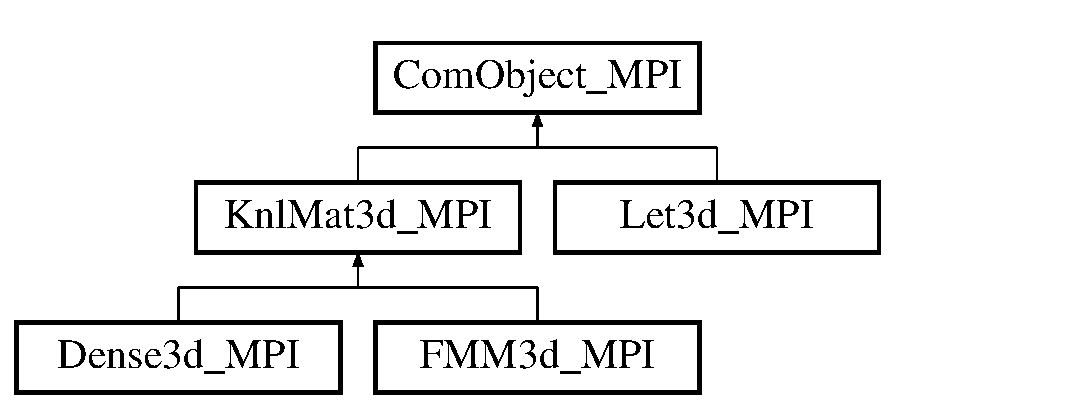
\includegraphics[height=3cm]{classComObject__MPI}
\end{center}
\end{figure}


\subsection{Detailed Description}
Com\-Object\_\-MPI class for communication purposes. Com\-Object stores basic message passing interface (mpi) information such as size and rank as defined in files included from using petsc $\ast$/. 



Definition at line 28 of file comobject\_\-mpi.hpp.\subsection*{Public Member Functions}
\begin{CompactItemize}
\item 
{\bf Com\-Object\_\-MPI} (const string \&prefix)
\item 
virtual {\bf $\sim$Com\-Object\_\-MPI} ()
\item 
const string \& {\bf prefix} ()
\item 
const MPI\_\-Comm \& {\bf mpi\-Comm} () const 
\item 
int {\bf mpi\-Rank} () const 
\item 
int {\bf mpi\-Size} () const 
\end{CompactItemize}
\subsection*{Protected Attributes}
\begin{CompactItemize}
\item 
string {\bf \_\-prefix}
\end{CompactItemize}


\subsection{Constructor \& Destructor Documentation}
\index{ComObject_MPI@{Com\-Object\_\-MPI}!ComObject_MPI@{ComObject\_\-MPI}}
\index{ComObject_MPI@{ComObject\_\-MPI}!ComObject_MPI@{Com\-Object\_\-MPI}}
\subsubsection{\setlength{\rightskip}{0pt plus 5cm}Com\-Object\_\-MPI::Com\-Object\_\-MPI (const string \& {\em prefix})\hspace{0.3cm}{\tt  [inline]}}\label{classComObject__MPI_77766478bbb936b1c62d5dc2dadd6788_77766478bbb936b1c62d5dc2dadd6788}


Initialize Com\-Object using string prefix 

Definition at line 35 of file comobject\_\-mpi.hpp.

\footnotesize\begin{verbatim}35 : _prefix(prefix) {;}
\end{verbatim}\normalsize 


\index{ComObject_MPI@{Com\-Object\_\-MPI}!~ComObject_MPI@{$\sim$ComObject\_\-MPI}}
\index{~ComObject_MPI@{$\sim$ComObject\_\-MPI}!ComObject_MPI@{Com\-Object\_\-MPI}}
\subsubsection{\setlength{\rightskip}{0pt plus 5cm}virtual Com\-Object\_\-MPI::$\sim$Com\-Object\_\-MPI ()\hspace{0.3cm}{\tt  [inline, virtual]}}\label{classComObject__MPI_b2929ed911fe3ec837f9654ff26a4249_b2929ed911fe3ec837f9654ff26a4249}




Definition at line 36 of file comobject\_\-mpi.hpp.

\footnotesize\begin{verbatim}36 {;}
\end{verbatim}\normalsize 




\subsection{Member Function Documentation}
\index{ComObject_MPI@{Com\-Object\_\-MPI}!mpiComm@{mpiComm}}
\index{mpiComm@{mpiComm}!ComObject_MPI@{Com\-Object\_\-MPI}}
\subsubsection{\setlength{\rightskip}{0pt plus 5cm}const MPI\_\-Comm\& Com\-Object\_\-MPI::mpi\-Comm () const\hspace{0.3cm}{\tt  [inline]}}\label{classComObject__MPI_dcb2a13b1c9df08fe9bc759bcfdb150e_dcb2a13b1c9df08fe9bc759bcfdb150e}


return MPI\_\-comm - set to PETSC\_\-COMM\_\-WORLD 

Definition at line 41 of file comobject\_\-mpi.hpp.

\footnotesize\begin{verbatim}41 { return PETSC_COMM_WORLD; }
\end{verbatim}\normalsize 


\index{ComObject_MPI@{Com\-Object\_\-MPI}!mpiRank@{mpiRank}}
\index{mpiRank@{mpiRank}!ComObject_MPI@{Com\-Object\_\-MPI}}
\subsubsection{\setlength{\rightskip}{0pt plus 5cm}int Com\-Object\_\-MPI::mpi\-Rank () const\hspace{0.3cm}{\tt  [inline]}}\label{classComObject__MPI_ae51fcdfaec9ca26c842280cf6b99aa9_ae51fcdfaec9ca26c842280cf6b99aa9}


return rank (id) of MPI\_\-Comm\_\-rank of PETSC\_\-COMM\_\-WORLD 

Definition at line 43 of file comobject\_\-mpi.hpp.

Referenced by Let3d\_\-MPI::print().

\footnotesize\begin{verbatim}43 { int rank; MPI_Comm_rank(PETSC_COMM_WORLD, &rank); return rank; }
\end{verbatim}\normalsize 


\index{ComObject_MPI@{Com\-Object\_\-MPI}!mpiSize@{mpiSize}}
\index{mpiSize@{mpiSize}!ComObject_MPI@{Com\-Object\_\-MPI}}
\subsubsection{\setlength{\rightskip}{0pt plus 5cm}int Com\-Object\_\-MPI::mpi\-Size () const\hspace{0.3cm}{\tt  [inline]}}\label{classComObject__MPI_1cb28464592687ed96a57c17cd3e0773_1cb28464592687ed96a57c17cd3e0773}


return size of MPI\_\-Comm\_\-size of PETSC\_\-COMM\_\-WORLD 

Definition at line 45 of file comobject\_\-mpi.hpp.

Referenced by FMM3d\_\-MPI::check().

\footnotesize\begin{verbatim}45 { int size; MPI_Comm_size(PETSC_COMM_WORLD, &size); return size; }
\end{verbatim}\normalsize 


\index{ComObject_MPI@{Com\-Object\_\-MPI}!prefix@{prefix}}
\index{prefix@{prefix}!ComObject_MPI@{Com\-Object\_\-MPI}}
\subsubsection{\setlength{\rightskip}{0pt plus 5cm}const string\& Com\-Object\_\-MPI::prefix ()\hspace{0.3cm}{\tt  [inline]}}\label{classComObject__MPI_8171d0694121d77c4bfba18e5745faa9_8171d0694121d77c4bfba18e5745faa9}


Return \_\-prefix string 

Definition at line 39 of file comobject\_\-mpi.hpp.

References \_\-prefix.

Referenced by Let3d\_\-MPI::setup(), and FMM3d\_\-MPI::setup().

\footnotesize\begin{verbatim}39 { return _prefix; }
\end{verbatim}\normalsize 




\subsection{Member Data Documentation}
\index{ComObject_MPI@{Com\-Object\_\-MPI}!_prefix@{\_\-prefix}}
\index{_prefix@{\_\-prefix}!ComObject_MPI@{Com\-Object\_\-MPI}}
\subsubsection{\setlength{\rightskip}{0pt plus 5cm}string {\bf Com\-Object\_\-MPI::\_\-prefix}\hspace{0.3cm}{\tt  [protected]}}\label{classComObject__MPI_b933f996cea3f524cf1514eb8539edfa_b933f996cea3f524cf1514eb8539edfa}


\_\-prefix is a string such as \char`\"{}fmm3d\_\-\char`\"{} which describes the type of object this is 

Definition at line 32 of file comobject\_\-mpi.hpp.

Referenced by prefix().

The documentation for this class was generated from the following file:\begin{CompactItemize}
\item 
fmm3d\_\-mpi/{\bf comobject\_\-mpi.hpp}\end{CompactItemize}

\section{Dense3d\_\-MPI Class Reference}
\label{classDense3d__MPI}\index{Dense3d_MPI@{Dense3d\_\-MPI}}
{\tt \#include $<$dense3d\_\-mpi.hpp$>$}

Inheritance diagram for Dense3d\_\-MPI::\begin{figure}[H]
\begin{center}
\leavevmode
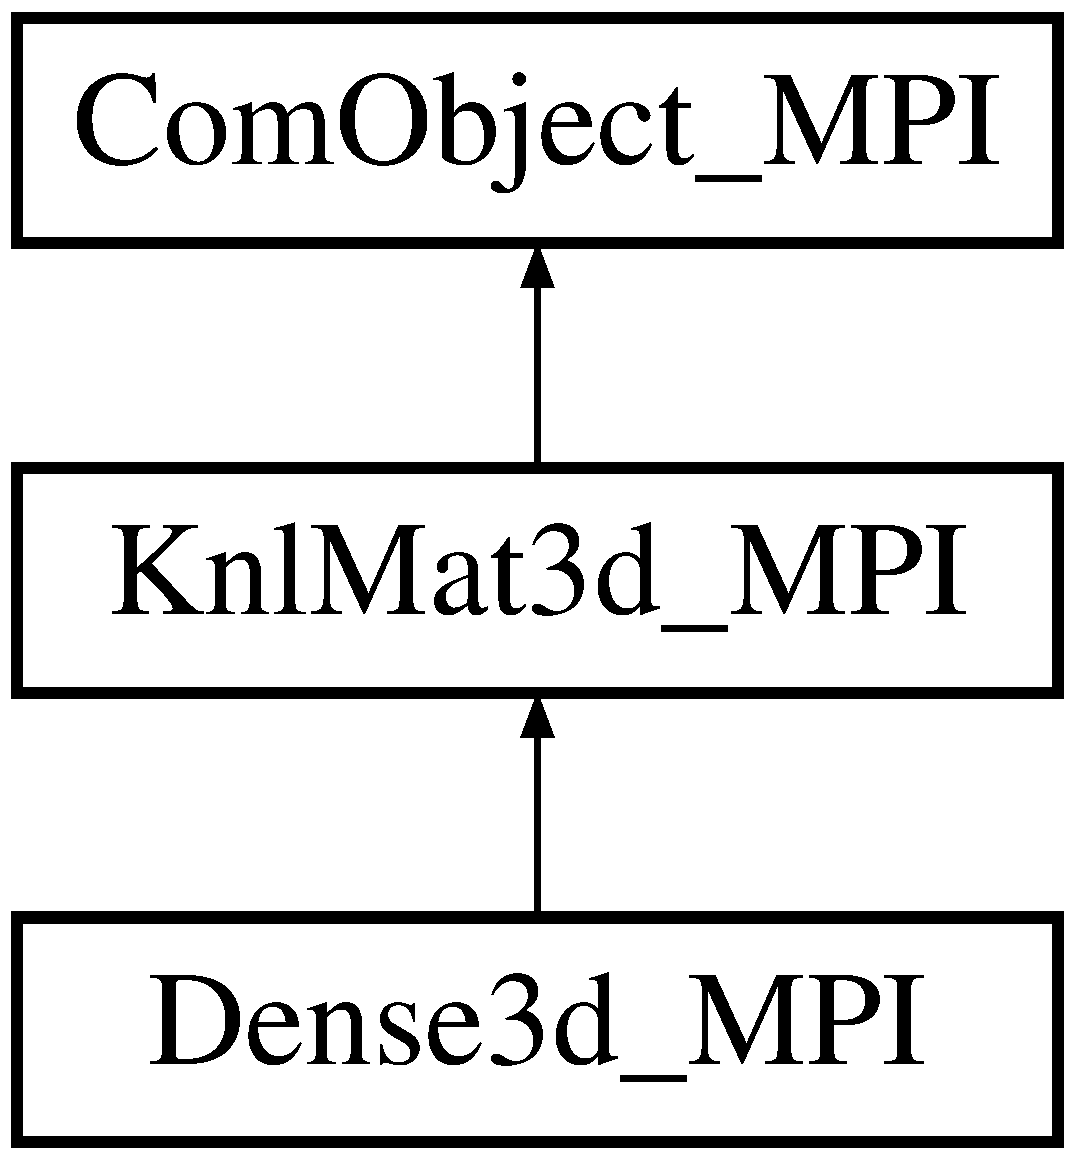
\includegraphics[height=3cm]{classDense3d__MPI}
\end{center}
\end{figure}


\subsection{Detailed Description}
Dense3d\_\-MPI implements setup and evaluate from {\bf Knl\-Mat3d\_\-MPI}{\rm (p.\,\pageref{classKnlMat3d__MPI})} the solver is a \char`\"{}dense\char`\"{} solver - meaning that fmm is not used, and the solution is \char`\"{}exact\char`\"{}. 



Definition at line 32 of file dense3d\_\-mpi.hpp.\subsection*{Public Member Functions}
\begin{CompactItemize}
\item 
{\bf Dense3d\_\-MPI} (const string \&p)
\item 
{\bf $\sim$Dense3d\_\-MPI} ()
\item 
int {\bf setup} ()
\item 
int {\bf evaluate} (Vec srcden, Vec trgval)
\end{CompactItemize}
\subsection*{Protected Attributes}
\begin{CompactItemize}
\item 
Vec {\bf \_\-src\-All\-Pos}
\item 
Vec {\bf \_\-src\-All\-Nor}
\end{CompactItemize}


\subsection{Constructor \& Destructor Documentation}
\index{Dense3d_MPI@{Dense3d\_\-MPI}!Dense3d_MPI@{Dense3d\_\-MPI}}
\index{Dense3d_MPI@{Dense3d\_\-MPI}!Dense3d_MPI@{Dense3d\_\-MPI}}
\subsubsection{\setlength{\rightskip}{0pt plus 5cm}Dense3d\_\-MPI::Dense3d\_\-MPI (const string \& {\em p})}\label{classDense3d__MPI_59f5eb1835ca9679e901a3ed7e570e99_59f5eb1835ca9679e901a3ed7e570e99}


construct Dense3d\_\-MPI using string prefix 

Definition at line 29 of file dense3d\_\-mpi.cpp.

\footnotesize\begin{verbatim}29                                        : 
30   KnlMat3d_MPI(p), _srcAllPos(NULL), _srcAllNor(NULL)
31 {
32 }
\end{verbatim}\normalsize 


\index{Dense3d_MPI@{Dense3d\_\-MPI}!~Dense3d_MPI@{$\sim$Dense3d\_\-MPI}}
\index{~Dense3d_MPI@{$\sim$Dense3d\_\-MPI}!Dense3d_MPI@{Dense3d\_\-MPI}}
\subsubsection{\setlength{\rightskip}{0pt plus 5cm}Dense3d\_\-MPI::$\sim$Dense3d\_\-MPI ()}\label{classDense3d__MPI_465a68462d0c24f1003e280546467196_465a68462d0c24f1003e280546467196}


call $\sim$Knl\-Mat3d\_\-MPI -$>$ $\sim$Com\-Object\_\-MPI.hpp 

Definition at line 34 of file dense3d\_\-mpi.cpp.

References \_\-src\-All\-Pos.

\footnotesize\begin{verbatim}35 {
36   if(_srcAllPos!=NULL) {         VecDestroy(_srcAllPos);  }
37   if(_srcAllNor!=NULL) {         VecDestroy(_srcAllNor);  }
38 }
\end{verbatim}\normalsize 




\subsection{Member Function Documentation}
\index{Dense3d_MPI@{Dense3d\_\-MPI}!evaluate@{evaluate}}
\index{evaluate@{evaluate}!Dense3d_MPI@{Dense3d\_\-MPI}}
\subsubsection{\setlength{\rightskip}{0pt plus 5cm}int Dense3d\_\-MPI::evaluate (Vec {\em srcden}, Vec {\em trgval})\hspace{0.3cm}{\tt  [virtual]}}\label{classDense3d__MPI_b6d6d5d529463497e5bed037a921cfc2_b6d6d5d529463497e5bed037a921cfc2}


Evaluate target values based on source densities and positions using direct evaluation 

Implements {\bf Knl\-Mat3d\_\-MPI} {\rm (p.\,\pageref{classKnlMat3d__MPI_abf7f0a466fbc47db0804a35093c819f_abf7f0a466fbc47db0804a35093c819f})}.

Definition at line 74 of file dense3d\_\-mpi.cpp.

References Knl\-Mat3d\_\-MPI::\_\-knl, \_\-src\-All\-Nor, \_\-src\-All\-Pos, Knl\-Mat3d\_\-MPI::\_\-src\-Nor, Knl\-Mat3d\_\-MPI::\_\-src\-Pos, Knl\-Mat3d\_\-MPI::\_\-trg\-Pos, Kernel3d\_\-MPI::build\-Knl\-Int\-Ctx(), Knl\-Mat3d\_\-MPI::dim(), p\-A, p\-C, Knl\-Mat3d\_\-MPI::proc\-Glb\-Num(), Knl\-Mat3d\_\-MPI::proc\-Lcl\-Num(), Knl\-Mat3d\_\-MPI::src\-DOF(), and Knl\-Mat3d\_\-MPI::trg\-DOF().

\footnotesize\begin{verbatim}75 {
76   //begin
77   // CHECK
78   pA(_srcPos!=NULL && _srcNor!=NULL && _trgPos!=NULL && srcDen!=NULL && trgVal!=NULL);
79   //-----------------------------------
80   int dim  = this->dim();
81   int srcDOF = this->srcDOF();
82   int trgDOF = this->trgDOF();
83   /* Get global number of source positions */
84   int srcGlbNum = procGlbNum(_srcPos);
85   /* Get local number of target positions */
86   int trgLclNum = procLclNum(_trgPos);
87   
88   Vec srcAllPos = _srcAllPos;
89   Vec srcAllNor = _srcAllNor;
90   Vec srcAllDen;
91   /* Create scatter context to scatter source densities to all processors */
92   {
93          VecScatter ctx;
94          pC( VecScatterCreateToAll(srcDen, &ctx, &srcAllDen) );
95          pC( VecScatterBegin(srcDen, srcAllDen, INSERT_VALUES, SCATTER_FORWARD, ctx) );
96          pC( VecScatterEnd(  srcDen, srcAllDen, INSERT_VALUES, SCATTER_FORWARD, ctx) );
97          pC( VecScatterDestroy(ctx) );
98   }
99   
100   Vec trgLclPos = _trgPos;
101   Vec trgLclVal =  trgVal;
102 
103   /* Create matrices for source positions, normals, densities.  See common/nummat.hpp for
104         * more information on matrices */
105   double* srcAllPosArr; pC( VecGetArray(srcAllPos, &srcAllPosArr) );
106   DblNumMat srcAllPosMat(dim, srcGlbNum, false, srcAllPosArr);
107   double* srcAllNorArr; pC( VecGetArray(srcAllNor, &srcAllNorArr) );
108   DblNumMat srcAllNorMat(dim, srcGlbNum, false, srcAllNorArr);
109   double* srcAllDenArr; pC( VecGetArray(srcAllDen, &srcAllDenArr) );
110   DblNumVec srcAllDenVec(srcDOF*srcGlbNum, false, srcAllDenArr);
111 
112   /* Create matrices for target positions and values */
113   double* trgLclPosArr; pC( VecGetArray(trgLclPos, &trgLclPosArr) );
114   DblNumMat trgLclPosMat(dim, trgLclNum, false, trgLclPosArr);
115   double* trgLclValArr; pC( VecGetArray(trgLclVal, &trgLclValArr) );
116   DblNumVec trgLclValVec(trgDOF*trgLclNum, false, trgLclValArr);
117 
118   /* Create an evaluation context and evaluate based on kernel type */
119   DblNumMat inter(trgDOF, srcGlbNum*srcDOF);
120   /* Do multiplication one line of the matrices at a time */
121   for(int i=0; i<trgLclNum; i++) {
122          DblNumMat onePosMat(dim, 1, false, trgLclPosMat.clmdata(i));
123          DblNumVec oneValVec(trgDOF, false, trgLclValVec.data()+trgDOF*i);
124          /* Create kernel multiplier context based on kernel type */
125          pC( _knl.buildKnlIntCtx(srcAllPosMat, srcAllNorMat, onePosMat, inter) );
126          /* Computes 1.0*inter*srcAllDenVec + 0.0*oneValVec = oneValVec */
127          pC( dgemv(1.0, inter, srcAllDenVec, 0.0, oneValVec) );
128   }
129   
130   pC( VecRestoreArray(srcAllPos, &srcAllPosArr) );
131   pC( VecRestoreArray(srcAllNor, &srcAllNorArr) );
132   pC( VecRestoreArray(srcAllDen, &srcAllDenArr) );
133   
134   pC( VecRestoreArray(trgLclPos, &trgLclPosArr) );
135   pC( VecRestoreArray(trgLclVal, &trgLclValArr) );
136   
137   pC( VecDestroy(srcAllDen) );
138   
139   return(0);
140 }
\end{verbatim}\normalsize 


\index{Dense3d_MPI@{Dense3d\_\-MPI}!setup@{setup}}
\index{setup@{setup}!Dense3d_MPI@{Dense3d\_\-MPI}}
\subsubsection{\setlength{\rightskip}{0pt plus 5cm}int Dense3d\_\-MPI::setup ()\hspace{0.3cm}{\tt  [virtual]}}\label{classDense3d__MPI_415266b005d267e801176f27c0434a50_415266b005d267e801176f27c0434a50}


Setup makes sure that all processor have the source positions and noremals scattered to them 

Implements {\bf Knl\-Mat3d\_\-MPI} {\rm (p.\,\pageref{classKnlMat3d__MPI_98f7aa1beebfd344710d076d3d6413a2_98f7aa1beebfd344710d076d3d6413a2})}.

Definition at line 45 of file dense3d\_\-mpi.cpp.

References \_\-\_\-FUNCT\_\-\_\-, \_\-src\-All\-Nor, \_\-src\-All\-Pos, Knl\-Mat3d\_\-MPI::\_\-src\-Nor, Knl\-Mat3d\_\-MPI::\_\-src\-Pos, Knl\-Mat3d\_\-MPI::\_\-trg\-Pos, p\-A, and p\-C.

\footnotesize\begin{verbatim}46 {
47   //begin
48   pA(_srcPos!=NULL && _srcNor!=NULL && _trgPos!=NULL);
49   //--------------------------------------------------------------------------
50   /* Create a Scatter context - copies all source position values to each processor
51         * See http://www-unix.mcs.anl.gov/petsc/petsc-as/snapshots/petsc-current/docs/manualpages/Vec/VecScatterCreateToAll.html */
52   {
53          VecScatter ctx;
54          pC( VecScatterCreateToAll(_srcPos, &ctx, &_srcAllPos) );
55          pC( VecScatterBegin(_srcPos, _srcAllPos, INSERT_VALUES, SCATTER_FORWARD, ctx) );
56          pC( VecScatterEnd(  _srcPos, _srcAllPos, INSERT_VALUES, SCATTER_FORWARD, ctx) );
57          pC( VecScatterDestroy(ctx) );
58   }
59   /* Create a Scatter context - copies all source normal values to each processor */
60   {
61          VecScatter ctx;
62          pC( VecScatterCreateToAll(_srcNor, &ctx, &_srcAllNor) );
63          pC( VecScatterBegin(_srcNor, _srcAllNor, INSERT_VALUES, SCATTER_FORWARD, ctx) );
64          pC( VecScatterEnd(  _srcNor, _srcAllNor, INSERT_VALUES, SCATTER_FORWARD, ctx) );
65          pC( VecScatterDestroy(ctx) );
66   }
67   return(0);
68 }
\end{verbatim}\normalsize 




\subsection{Member Data Documentation}
\index{Dense3d_MPI@{Dense3d\_\-MPI}!_srcAllNor@{\_\-srcAllNor}}
\index{_srcAllNor@{\_\-srcAllNor}!Dense3d_MPI@{Dense3d\_\-MPI}}
\subsubsection{\setlength{\rightskip}{0pt plus 5cm}Vec {\bf Dense3d\_\-MPI::\_\-src\-All\-Nor}\hspace{0.3cm}{\tt  [protected]}}\label{classDense3d__MPI_db2ec95209a80ecf4e75545dbe1bd00d_db2ec95209a80ecf4e75545dbe1bd00d}


all source normals 

Definition at line 39 of file dense3d\_\-mpi.hpp.

Referenced by evaluate(), and setup().\index{Dense3d_MPI@{Dense3d\_\-MPI}!_srcAllPos@{\_\-srcAllPos}}
\index{_srcAllPos@{\_\-srcAllPos}!Dense3d_MPI@{Dense3d\_\-MPI}}
\subsubsection{\setlength{\rightskip}{0pt plus 5cm}Vec {\bf Dense3d\_\-MPI::\_\-src\-All\-Pos}\hspace{0.3cm}{\tt  [protected]}}\label{classDense3d__MPI_864bdce428c7c15d43e08e6733357f13_864bdce428c7c15d43e08e6733357f13}


all source positions 

Definition at line 37 of file dense3d\_\-mpi.hpp.

Referenced by evaluate(), setup(), and $\sim$Dense3d\_\-MPI().

The documentation for this class was generated from the following files:\begin{CompactItemize}
\item 
fmm3d\_\-mpi/{\bf dense3d\_\-mpi.hpp}\item 
fmm3d\_\-mpi/{\bf dense3d\_\-mpi.cpp}\end{CompactItemize}

\section{FMM3d\_\-MPI Class Reference}
\label{classFMM3d__MPI}\index{FMM3d_MPI@{FMM3d\_\-MPI}}
{\tt \#include $<$fmm3d\_\-mpi.hpp$>$}

Inheritance diagram for FMM3d\_\-MPI::\begin{figure}[H]
\begin{center}
\leavevmode
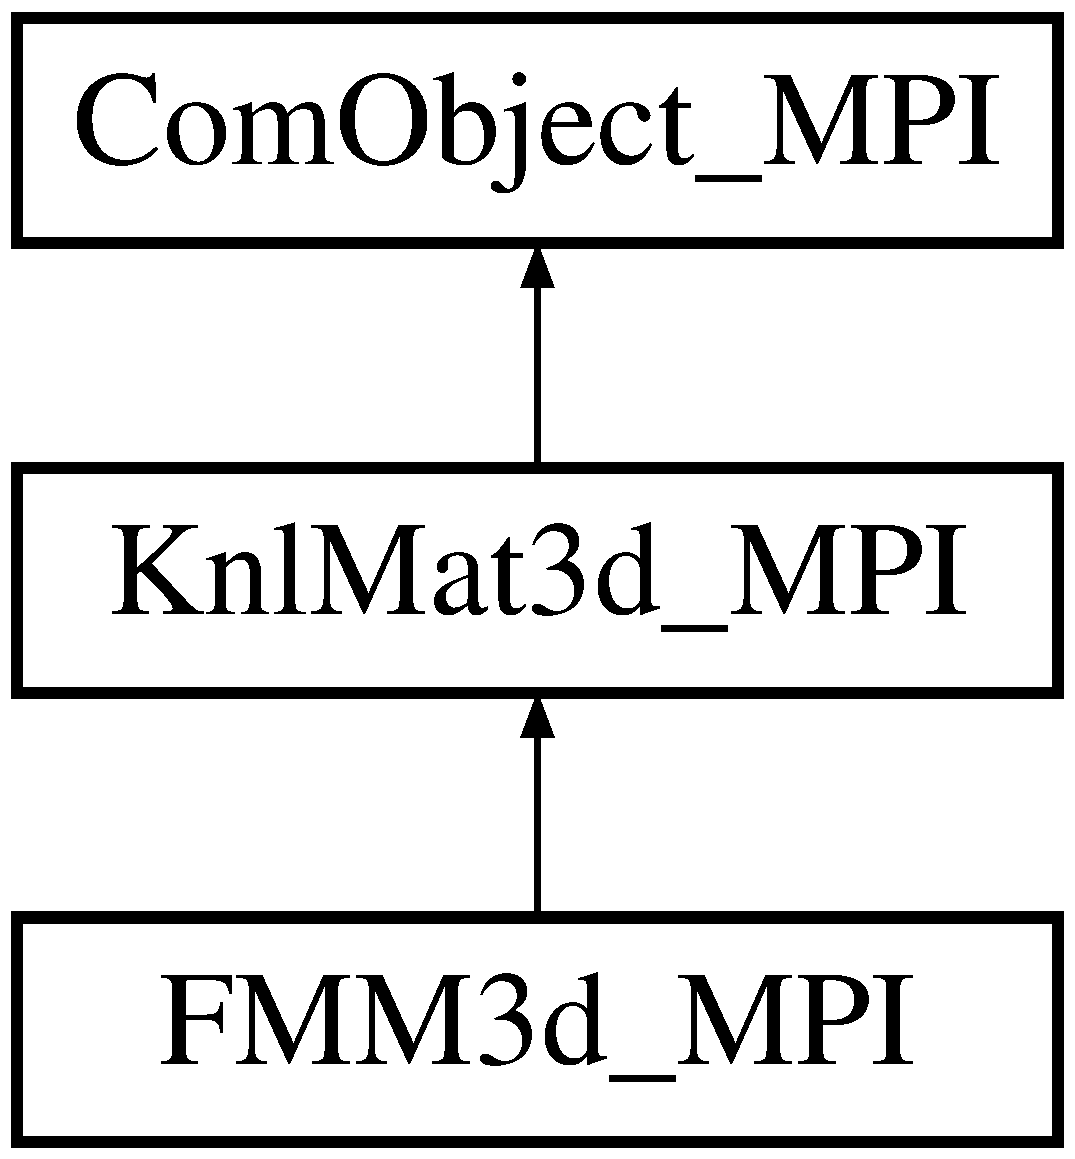
\includegraphics[height=3cm]{classFMM3d__MPI}
\end{center}
\end{figure}


\subsection{Detailed Description}
FMM3d\_\-MPI inherits from {\bf Knl\-Mat3d\_\-MPI}{\rm (p.\,\pageref{classKnlMat3d__MPI})}. Specific information for computing and using FMM are implemented here. Specifically, setup and evaluate and inherits source positions, etc. See {\bf knlmat3d\_\-mpi.hpp}{\rm (p.\,\pageref{knlmat3d__mpi_8hpp})} for more information. 



Definition at line 36 of file fmm3d\_\-mpi.hpp.\subsection*{Public Types}
\begin{CompactItemize}
\item 
typedef pair$<$ int, int $>$ {\bf intpair}
\item 
enum \{ {\bf UE} = 0, 
{\bf UC} = 1, 
{\bf DE} = 2, 
{\bf DC} = 3
 \}
\end{CompactItemize}
\subsection*{Public Member Functions}
\begin{CompactItemize}
\item 
{\bf FMM3d\_\-MPI} (const string \&p)
\item 
{\bf $\sim$FMM3d\_\-MPI} ()
\item 
Point3 \& {\bf ctr} ()
\item 
int \& {\bf root\-Level} ()
\item 
int \& {\bf np} ()
\item 
int {\bf setup} ()
\item 
int {\bf evaluate} (Vec src\-Den, Vec trg\-Val)
\item 
int {\bf check} (Vec src\-Den, Vec trg\-Val, int numchk, double \&rerr)
\item 
{\bf Let3d\_\-MPI} $\ast$ {\bf let} ()
\item 
{\bf Mat\-Mgnt3d\_\-MPI} $\ast$ {\bf matmgnt} ()
\item 
{\bf Node} \& {\bf node} (int g\-Node\-Idx)
\end{CompactItemize}
\subsection*{Protected Member Functions}
\begin{CompactItemize}
\item 
int {\bf dat\-Sze} (int tp)
\item 
int {\bf Src\-Equ2Trg\-Chk\_\-dgemv} (const Dbl\-Num\-Mat \&src\-Pos, const Dbl\-Num\-Mat \&src\-Nor, const Dbl\-Num\-Mat \&trg\-Pos, const Dbl\-Num\-Vec \&src\-Den, Dbl\-Num\-Vec \&trg\-Val)
\item 
int {\bf Src\-Equ2Upw\-Chk\_\-dgemv} (const Dbl\-Num\-Mat \&src\-Pos, const Dbl\-Num\-Mat \&src\-Nor, Point3 trgctr, double trgrad, const Dbl\-Num\-Vec \&src\-Den, Dbl\-Num\-Vec \&trg\-Val)
\item 
int {\bf Src\-Equ2Dwn\-Chk\_\-dgemv} (const Dbl\-Num\-Mat \&src\-Pos, const Dbl\-Num\-Mat \&src\-Nor, Point3 trgctr, double trgrad, const Dbl\-Num\-Vec \&src\-Den, Dbl\-Num\-Vec \&trg\-Val)
\item 
int {\bf Dwn\-Equ2Trg\-Chk\_\-dgemv} (Point3 srcctr, double srcrad, const Dbl\-Num\-Mat \&trg\-Pos, const Dbl\-Num\-Vec \&src\-Den, Dbl\-Num\-Vec \&trg\-Val)
\item 
int {\bf Upw\-Equ2Trg\-Chk\_\-dgemv} (Point3 srcctr, double srcrad, const Dbl\-Num\-Mat \&trg\-Pos, const Dbl\-Num\-Vec \&src\-Den, Dbl\-Num\-Vec \&trg\-Val)
\item 
Dbl\-Num\-Mat {\bf ctb\-Src\-Exa\-Pos} (int g\-Node\-Idx)
\item 
Dbl\-Num\-Mat {\bf ctb\-Src\-Exa\-Nor} (int g\-Node\-Idx)
\item 
Dbl\-Num\-Vec {\bf ctb\-Src\-Exa\-Den} (int g\-Node\-Idx)
\item 
Dbl\-Num\-Vec {\bf ctb\-Src\-Upw\-Equ\-Den} (int g\-Node\-Idx)
\item 
Dbl\-Num\-Vec {\bf ctb\-Src\-Upw\-Chk\-Val} (int g\-Node\-Idx)
\item 
Dbl\-Num\-Mat {\bf usr\-Src\-Exa\-Pos} (int g\-Node\-Idx)
\item 
Dbl\-Num\-Mat {\bf usr\-Src\-Exa\-Nor} (int g\-Node\-Idx)
\item 
Dbl\-Num\-Vec {\bf usr\-Src\-Exa\-Den} (int g\-Node\-Idx)
\item 
Dbl\-Num\-Vec {\bf usr\-Src\-Upw\-Equ\-Den} (int g\-Node\-Idx)
\item 
Dbl\-Num\-Mat {\bf eva\-Trg\-Exa\-Pos} (int g\-Node\-Idx)
\item 
Dbl\-Num\-Vec {\bf eva\-Trg\-Exa\-Val} (int g\-Node\-Idx)
\item 
Dbl\-Num\-Vec {\bf eva\-Trg\-Dwn\-Equ\-Den} (int g\-Node\-Idx)
\item 
Dbl\-Num\-Vec {\bf eva\-Trg\-Dwn\-Chk\-Val} (int g\-Node\-Idx)
\end{CompactItemize}
\subsection*{Protected Attributes}
\begin{CompactItemize}
\item 
Point3 {\bf \_\-ctr}
\item 
int {\bf \_\-root\-Level}
\item 
int {\bf \_\-np}
\item 
{\bf Let3d\_\-MPI} $\ast$ {\bf \_\-let}
\item 
{\bf Mat\-Mgnt3d\_\-MPI} $\ast$ {\bf \_\-matmgnt}
\item 
vector$<$ {\bf Node} $>$ {\bf \_\-node\-Vec}
\item 
Vec {\bf \_\-glb\-Src\-Exa\-Pos}
\item 
Vec {\bf \_\-glb\-Src\-Exa\-Nor}
\item 
Vec {\bf \_\-glb\-Src\-Exa\-Den}
\item 
Vec {\bf \_\-glb\-Src\-Upw\-Equ\-Den}
\item 
Vec {\bf \_\-ctb\-Src\-Exa\-Pos}
\item 
Vec {\bf \_\-ctb\-Src\-Exa\-Nor}
\item 
Vec {\bf \_\-ctb\-Src\-Exa\-Den}
\item 
Vec {\bf \_\-ctb\-Src\-Upw\-Equ\-Den}
\item 
Vec {\bf \_\-ctb\-Src\-Upw\-Chk\-Val}
\item 
Vec\-Scatter {\bf \_\-ctb2Glb\-Src\-Exa\-Pos}
\item 
Vec\-Scatter {\bf \_\-ctb2Glb\-Src\-Exa\-Den}
\item 
Vec\-Scatter {\bf \_\-ctb2Glb\-Src\-Upw\-Equ\-Den}
\item 
Vec {\bf \_\-eva\-Trg\-Exa\-Pos}
\item 
Vec {\bf \_\-eva\-Trg\-Exa\-Val}
\item 
Vec {\bf \_\-eva\-Trg\-Dwn\-Equ\-Den}
\item 
Vec {\bf \_\-eva\-Trg\-Dwn\-Chk\-Val}
\item 
Vec {\bf \_\-usr\-Src\-Exa\-Pos}
\item 
Vec {\bf \_\-usr\-Src\-Exa\-Nor}
\item 
Vec {\bf \_\-usr\-Src\-Exa\-Den}
\item 
Vec {\bf \_\-usr\-Src\-Upw\-Equ\-Den}
\item 
Vec\-Scatter {\bf \_\-usr2Glb\-Src\-Exa\-Pos}
\item 
Vec\-Scatter {\bf \_\-usr2Glb\-Src\-Exa\-Den}
\item 
Vec\-Scatter {\bf \_\-usr2Glb\-Src\-Upw\-Equ\-Den}
\item 
{\bf Kernel3d\_\-MPI} {\bf \_\-knl\_\-mm}
\end{CompactItemize}
\subsection*{Classes}
\begin{CompactItemize}
\item 
class {\bf Node}
\begin{CompactList}\small\item\em {\bf Node}{\rm (p.\,\pageref{classFMM3d__MPI_1_1Node})} class for {\bf FMM3d\_\-MPI}{\rm (p.\,\pageref{classFMM3d__MPI})} stores access functions to {\bf Node\-Ext}{\rm (p.\,\pageref{classFMM3d__MPI_1_1NodeExt})}. \item\end{CompactList}\item 
class {\bf Node\-Ext}
\begin{CompactList}\small\item\em Extra node information. Different from {\bf Let3d\_\-MPI::Node\-Ext}{\rm (p.\,\pageref{classLet3d__MPI_1_1NodeExt})}. \item\end{CompactList}\end{CompactItemize}


\subsection{Member Typedef Documentation}
\index{FMM3d_MPI@{FMM3d\_\-MPI}!intpair@{intpair}}
\index{intpair@{intpair}!FMM3d_MPI@{FMM3d\_\-MPI}}
\subsubsection{\setlength{\rightskip}{0pt plus 5cm}typedef pair$<$int,int$>$ {\bf FMM3d\_\-MPI::intpair}}\label{classFMM3d__MPI_516fcca2e14cd2e14fd71db54824f696_516fcca2e14cd2e14fd71db54824f696}




Definition at line 39 of file fmm3d\_\-mpi.hpp.

\subsection{Member Enumeration Documentation}
\subsubsection{\setlength{\rightskip}{0pt plus 5cm}anonymous enum}\label{classFMM3d__MPI_dca29a1140aadadfd92b34a02fa516ef_dca29a1140aadadfd92b34a02fa516ef}


\begin{Desc}
\item[Enumerator: ]\par
\begin{description}
\index{UE@{UE}!FMM3d_MPI@{FMM3d\_\-MPI}}\index{FMM3d_MPI@{FMM3d\_\-MPI}!UE@{UE}}\item[{\em 
UE\label{classFMM3d__MPI_dca29a1140aadadfd92b34a02fa516ef_dca29a1140aadadfd92b34a02fa516ef0612e93d65abcdaeed533a0876474251}
}]Upward Equivalent \index{UC@{UC}!FMM3d_MPI@{FMM3d\_\-MPI}}\index{FMM3d_MPI@{FMM3d\_\-MPI}!UC@{UC}}\item[{\em 
UC\label{classFMM3d__MPI_dca29a1140aadadfd92b34a02fa516ef_dca29a1140aadadfd92b34a02fa516ef6a2fb30a2dacdda4d74122697262a8b7}
}]Upward Check \index{DE@{DE}!FMM3d_MPI@{FMM3d\_\-MPI}}\index{FMM3d_MPI@{FMM3d\_\-MPI}!DE@{DE}}\item[{\em 
DE\label{classFMM3d__MPI_dca29a1140aadadfd92b34a02fa516ef_dca29a1140aadadfd92b34a02fa516ef3a52f3c22ed6fcde5bf696a6c02c9e73}
}]Downward Equivalent \index{DC@{DC}!FMM3d_MPI@{FMM3d\_\-MPI}}\index{FMM3d_MPI@{FMM3d\_\-MPI}!DC@{DC}}\item[{\em 
DC\label{classFMM3d__MPI_dca29a1140aadadfd92b34a02fa516ef_dca29a1140aadadfd92b34a02fa516efcf75e54791dd1f49f918345fdfe2430b}
}]Downward Check \end{description}
\end{Desc}



Definition at line 40 of file fmm3d\_\-mpi.hpp.

\footnotesize\begin{verbatim}40        {          UE=0, UC=1, DE=2, DC=3,  };
\end{verbatim}\normalsize 




\subsection{Constructor \& Destructor Documentation}
\index{FMM3d_MPI@{FMM3d\_\-MPI}!FMM3d_MPI@{FMM3d\_\-MPI}}
\index{FMM3d_MPI@{FMM3d\_\-MPI}!FMM3d_MPI@{FMM3d\_\-MPI}}
\subsubsection{\setlength{\rightskip}{0pt plus 5cm}FMM3d\_\-MPI::FMM3d\_\-MPI (const string \& {\em p})}\label{classFMM3d__MPI_9f48ad5b4ec95878d1bb32a181525789_9f48ad5b4ec95878d1bb32a181525789}


Initialize FMM3d\_\-MPI with string. Calls constructor from {\bf Knl\-Mat3d\_\-MPI}{\rm (p.\,\pageref{classKnlMat3d__MPI})}, and initializes are vectors here to NULL and values to zero. Center defaults to (0,0,0), root\-Level to 0, and np to 6 

Definition at line 31 of file fmm3d\_\-mpi.cpp.

\footnotesize\begin{verbatim}31                                    :
32   KnlMat3d_MPI(p), _ctr(0,0,0), _rootLevel(0),
33   _np(6),
34   _let(NULL), _matmgnt(NULL),
35   _glbSrcExaPos(NULL), _glbSrcExaNor(NULL), _glbSrcExaDen(NULL), _glbSrcUpwEquDen(NULL),
36   _ctbSrcExaPos(NULL), _ctbSrcExaNor(NULL), _ctbSrcExaDen(NULL), _ctbSrcUpwEquDen(NULL),
37   _ctbSrcUpwChkVal(NULL), _ctb2GlbSrcExaPos(NULL), _ctb2GlbSrcExaDen(NULL), _ctb2GlbSrcUpwEquDen(NULL),
38   _evaTrgExaPos(NULL), _evaTrgExaVal(NULL), _evaTrgDwnEquDen(NULL), _evaTrgDwnChkVal(NULL),
39   _usrSrcExaPos(NULL), _usrSrcExaNor(NULL), _usrSrcExaDen(NULL), _usrSrcUpwEquDen(NULL),
40   _usr2GlbSrcExaPos(NULL), _usr2GlbSrcExaDen(NULL), _usr2GlbSrcUpwEquDen(NULL)
41 {
42 }

\end{verbatim}\normalsize 


\index{FMM3d_MPI@{FMM3d\_\-MPI}!~FMM3d_MPI@{$\sim$FMM3d\_\-MPI}}
\index{~FMM3d_MPI@{$\sim$FMM3d\_\-MPI}!FMM3d_MPI@{FMM3d\_\-MPI}}
\subsubsection{\setlength{\rightskip}{0pt plus 5cm}FMM3d\_\-MPI::$\sim$FMM3d\_\-MPI ()}\label{classFMM3d__MPI_2cb06cc1c18cba63ed0226e5e691b3ca_2cb06cc1c18cba63ed0226e5e691b3ca}




Definition at line 45 of file fmm3d\_\-mpi.cpp.

References \_\-glb\-Src\-Exa\-Nor, \_\-glb\-Src\-Exa\-Pos, and \_\-let.

\footnotesize\begin{verbatim}46 {
47   if(_let!=NULL)         delete _let;
48   
49   if(_glbSrcExaPos!=NULL) { iC( VecDestroy(_glbSrcExaPos) ); _glbSrcExaPos=NULL; }
50   if(_glbSrcExaNor!=NULL) { iC( VecDestroy(_glbSrcExaNor) ); _glbSrcExaPos=NULL; }
51   if(_glbSrcExaDen!=NULL) { iC( VecDestroy(_glbSrcExaDen) ); _glbSrcExaDen=NULL; }
52   if(_glbSrcUpwEquDen!=NULL) { iC( VecDestroy(_glbSrcUpwEquDen) ); _glbSrcUpwEquDen=NULL; }
53   
54   if(_ctbSrcExaPos!=NULL) { iC( VecDestroy(_ctbSrcExaPos) ); _ctbSrcExaPos=NULL; }
55   if(_ctbSrcExaNor!=NULL) { iC( VecDestroy(_ctbSrcExaNor) ); _ctbSrcExaNor=NULL; }
56   if(_ctbSrcExaDen!=NULL) { iC( VecDestroy(_ctbSrcExaDen) ); _ctbSrcExaDen=NULL; }
57   if(_ctbSrcUpwEquDen!=NULL) { iC( VecDestroy(_ctbSrcUpwEquDen) ); _ctbSrcUpwEquDen=NULL; }
58   if(_ctbSrcUpwChkVal!=NULL) { iC( VecDestroy(_ctbSrcUpwChkVal) ); _ctbSrcUpwChkVal=NULL; }
59   if(_ctb2GlbSrcExaPos!=NULL) { iC( VecScatterDestroy(_ctb2GlbSrcExaPos) ); _ctb2GlbSrcExaPos=NULL; }
60   if(_ctb2GlbSrcExaDen!=NULL) { iC( VecScatterDestroy(_ctb2GlbSrcExaDen) ); _ctb2GlbSrcExaDen=NULL; }
61   if(_ctb2GlbSrcUpwEquDen!=NULL) { iC( VecScatterDestroy(_ctb2GlbSrcUpwEquDen) ); _ctb2GlbSrcUpwEquDen=NULL; }
62   
63   if(_evaTrgExaPos!=NULL) { iC( VecDestroy(_evaTrgExaPos) ); _evaTrgExaPos=NULL; }
64   if(_evaTrgExaVal!=NULL) { iC( VecDestroy(_evaTrgExaVal) ); _evaTrgExaVal=NULL; }
65   if(_evaTrgDwnEquDen!=NULL) { iC( VecDestroy(_evaTrgDwnEquDen) ); _evaTrgDwnEquDen=NULL; }
66   if(_evaTrgDwnChkVal!=NULL) { iC( VecDestroy(_evaTrgDwnChkVal) ); _evaTrgDwnChkVal=NULL; }
67   
68   if(_usrSrcExaPos!=NULL) { iC( VecDestroy(_usrSrcExaPos) ); _usrSrcExaPos=NULL; }
69   if(_usrSrcExaNor!=NULL) { iC( VecDestroy(_usrSrcExaNor) ); _usrSrcExaNor=NULL; }
70   if(_usrSrcExaDen!=NULL) { iC( VecDestroy(_usrSrcExaDen) ); _usrSrcExaDen=NULL; }
71   if(_usrSrcUpwEquDen!=NULL) { iC( VecDestroy(_usrSrcUpwEquDen) ); _usrSrcUpwEquDen=NULL; }
72   if(_usr2GlbSrcExaPos!=NULL) { iC( VecScatterDestroy(_usr2GlbSrcExaPos) ); _usr2GlbSrcExaPos=NULL; }
73   if(_usr2GlbSrcExaDen!=NULL) { iC( VecScatterDestroy(_usr2GlbSrcExaDen) ); _usr2GlbSrcExaDen=NULL; }
74   if(_usr2GlbSrcUpwEquDen!=NULL) { iC( VecScatterDestroy(_usr2GlbSrcUpwEquDen) ); _usr2GlbSrcUpwEquDen=NULL; }
75 }
\end{verbatim}\normalsize 




\subsection{Member Function Documentation}
\index{FMM3d_MPI@{FMM3d\_\-MPI}!check@{check}}
\index{check@{check}!FMM3d_MPI@{FMM3d\_\-MPI}}
\subsubsection{\setlength{\rightskip}{0pt plus 5cm}int FMM3d\_\-MPI::check (Vec {\em src\-Den}, Vec {\em trg\-Val}, int {\em numchk}, double \& {\em rerr})}\label{classFMM3d__MPI_d2aa9de21b49559ceb1eb86a90536758_d2aa9de21b49559ceb1eb86a90536758}


check function, returns relative error. Detailed in fmm3d\_\-mpi\_\-check.cpp 

Definition at line 34 of file fmm3d\_\-check\_\-mpi.cpp.

References Knl\-Mat3d\_\-MPI::\_\-src\-Pos, Knl\-Mat3d\_\-MPI::\_\-trg\-Pos, Knl\-Mat3d\_\-MPI::dim(), Com\-Object\_\-MPI::mpi\-Size(), p\-A, Knl\-Mat3d\_\-MPI::proc\-Lcl\-Num(), Knl\-Mat3d\_\-MPI::src\-DOF(), and Knl\-Mat3d\_\-MPI::trg\-DOF().

\footnotesize\begin{verbatim}35 {
36   //begin
37   pA(procLclNum(_trgPos)>0); //have things to check
38   //pC( PetscPrintf(mpiComm(), "checking.........\n") );
39   int dim = this->dim();
40   int srcDOF = this->srcDOF();
41   int trgDOF = this->trgDOF();
42   int slclnum = procLclNum(_srcPos);
43   int tlclnum = procLclNum(_trgPos);   //int lclnum = this->lclnum();
44   
45   //1. select point to check
46   int ttlChk = numChk*mpiSize();
47   vector<int> chkVec(numChk);
48   for(int k=0; k<numChk; k++) {
49          chkVec[k] = int( floor(drand48()*tlclnum) );
50          pA(chkVec[k]>=0 && chkVec[k]<tlclnum);
51   }
52   pC( MPI_Barrier(mpiComm()) );
53   
54   Vec chkPos; pC( VecCreateMPI(mpiComm(), numChk*dim,  ttlChk*dim,  &chkPos) ); //check position
55   Vec chkVal; pC( VecCreateMPI(mpiComm(), numChk*trgDOF, ttlChk*trgDOF, &chkVal) ); //check value
56   Vec chkDen; pC( VecCreateMPI(mpiComm(), numChk*trgDOF, ttlChk*trgDOF, &chkDen) ); //check density
57   
58   double* posArr; pC( VecGetArray(_trgPos, &posArr) );
59   double* valArr; pC( VecGetArray( trgVal, &valArr) );
60   double* chkPosArr; pC( VecGetArray(chkPos, &chkPosArr) );
61   double* chkValArr; pC( VecGetArray(chkVal, &chkValArr) );
62   for(int k=0; k<numChk; k++) {
63          for(int i=0; i<dim; i++)
64                 chkPosArr[ k*dim+i  ] = posArr[ chkVec[k]*dim+i  ];
65          for(int i=0; i<trgDOF;i++)
66                 chkValArr[ k*trgDOF+i ] = valArr[ chkVec[k]*trgDOF+i ];
67   } 
68   pC( VecRestoreArray(_trgPos, &posArr) );
69   pC( VecRestoreArray( trgVal, &valArr) );
70   pC( VecRestoreArray(chkPos, &chkPosArr) );
71   pC( VecRestoreArray(chkVal, &chkValArr) );
72   
73   //2. compute and gather
74   Vec allChkPos;
75   {
76          VecScatter ctx;  pC( VecScatterCreateToAll(chkPos, &ctx, &allChkPos) );
77          pC( VecScatterBegin(chkPos, allChkPos, INSERT_VALUES, SCATTER_FORWARD, ctx) );
78          pC( VecScatterEnd(  chkPos, allChkPos, INSERT_VALUES, SCATTER_FORWARD, ctx) );
79          pC( VecScatterDestroy(ctx) );
80   }
81   Vec allChkDen; pC( VecCreateSeq(PETSC_COMM_SELF, ttlChk*trgDOF, &allChkDen) );
82   Vec glbChkDen; pC( VecCreateSeq(PETSC_COMM_SELF, ttlChk*trgDOF, &glbChkDen) );
83   
84   double* lclSrcPosArr; pC( VecGetArray(_srcPos, &lclSrcPosArr) );
85   double* lclSrcNorArr; pC( VecGetArray(_srcNor, &lclSrcNorArr) );
86   double* lclSrcDenArr; pC( VecGetArray( srcDen, &lclSrcDenArr) );
87   double* allChkPosArr; pC( VecGetArray(allChkPos, &allChkPosArr) );
88   double* allChkDenArr; pC( VecGetArray(allChkDen, &allChkDenArr) );
89   double* glbChkDenArr; pC( VecGetArray(glbChkDen, &glbChkDenArr) );
90   
91   DblNumMat lclSrcPosMat(dim, slclnum, false, lclSrcPosArr);
92   DblNumMat lclSrcNorMat(dim, slclnum, false, lclSrcNorArr);
93   DblNumVec lclSrcDenVec(srcDOF*slclnum, false, lclSrcDenArr);
94   DblNumMat allChkPosMat(dim,  ttlChk, false, allChkPosArr);
95   DblNumVec allChkDenVec(trgDOF* ttlChk, false, allChkDenArr);
96   
97   DblNumMat inter(trgDOF, slclnum*srcDOF);
98   for(int i=0; i<ttlChk; i++) {
99          DblNumMat oneChkPosMat(dim, 1, false, allChkPosMat.clmdata(i));
100          DblNumVec oneChkDenVec(trgDOF, false, allChkDenVec.data()+i*trgDOF);
101          pC( _knl.buildKnlIntCtx(lclSrcPosMat, lclSrcNorMat, oneChkPosMat, inter) );
102          pC( dgemv(1.0, inter, lclSrcDenVec, 0.0, oneChkDenVec) );
103   }
104   
105   pC( MPI_Barrier(mpiComm()) );
106   pC( MPI_Allreduce(allChkDenArr, glbChkDenArr, ttlChk*trgDOF, MPI_DOUBLE, MPI_SUM, mpiComm()) );
107   
108   //3. distribute to individual
109   double* lclChkDenArr; pC( VecGetArray(chkDen, &lclChkDenArr) );
110   void* dst = (void*)lclChkDenArr;
111   void* src = (void*)(glbChkDenArr + mpiRank()*numChk*trgDOF);  
112   memcpy(dst, src, sizeof(double)*numChk*trgDOF);
113   pC( VecRestoreArray(chkDen, &lclChkDenArr) );
114   
115   pC( VecRestoreArray(_srcPos, &lclSrcPosArr) );
116   pC( VecRestoreArray(_srcNor, &lclSrcNorArr) );
117   pC( VecRestoreArray( srcDen, &lclSrcDenArr) );
118   pC( VecRestoreArray(allChkPos, &allChkPosArr) );
119   pC( VecRestoreArray(allChkDen, &allChkDenArr) );
120   pC( VecRestoreArray(glbChkDen, &glbChkDenArr) );
121   
122   pC( VecDestroy(allChkPos) );
123   pC( VecDestroy(allChkDen) );
124   pC( VecDestroy(glbChkDen) );
125   
126   PetscScalar mone = -1.0;
127   pC( VecAXPY(chkVal, mone, chkDen) ); //chkVal now is the error - HARPER:  In correct order??
128   double nerr, npot;
129   pC( VecNorm(chkVal, NORM_2, &nerr) );
130   pC( VecNorm(chkDen, NORM_2, &npot) );
131   
132   rerr = nerr/npot;//pC( PetscPrintf(mpiComm(), "Error %e, %e %e\n", nerr/npot, nerr, npot) );
133   
134   pC( VecDestroy(chkPos) );
135   pC( VecDestroy(chkVal) );
136   pC( VecDestroy(chkDen) );
137   
138   return(0);
139 }
\end{verbatim}\normalsize 


\index{FMM3d_MPI@{FMM3d\_\-MPI}!ctbSrcExaDen@{ctbSrcExaDen}}
\index{ctbSrcExaDen@{ctbSrcExaDen}!FMM3d_MPI@{FMM3d\_\-MPI}}
\subsubsection{\setlength{\rightskip}{0pt plus 5cm}Dbl\-Num\-Vec FMM3d\_\-MPI::ctb\-Src\-Exa\-Den (int {\em g\-Node\-Idx})\hspace{0.3cm}{\tt  [protected]}}\label{classFMM3d__MPI_99138c2857a67a0f74ce4f752045aab1_99138c2857a67a0f74ce4f752045aab1}


Return vector of contributor exact source densities for a specific node - gets information from \_\-let 

Definition at line 273 of file fmm3d\_\-mpi.cpp.

References \_\-ctb\-Src\-Exa\-Den, \_\-let, Let3d\_\-MPI::Node::ctb\-Src\-Exa\-Beg(), Let3d\_\-MPI::Node::ctb\-Src\-Exa\-Num(), Let3d\_\-MPI::node(), node(), and Knl\-Mat3d\_\-MPI::src\-DOF().

Referenced by evaluate().

\footnotesize\begin{verbatim}274 {
275   Let3d_MPI::Node& node = _let->node(gNodeIdx);
276   int beg = node.ctbSrcExaBeg();
277   int num = node.ctbSrcExaNum();
278   double* arr;     VecGetArray(    _ctbSrcExaDen, &arr);
279   double* buf=arr; VecRestoreArray(_ctbSrcExaDen, &arr);
280   return DblNumVec(srcDOF()*num, false, buf+beg*srcDOF());
281 }
\end{verbatim}\normalsize 


\index{FMM3d_MPI@{FMM3d\_\-MPI}!ctbSrcExaNor@{ctbSrcExaNor}}
\index{ctbSrcExaNor@{ctbSrcExaNor}!FMM3d_MPI@{FMM3d\_\-MPI}}
\subsubsection{\setlength{\rightskip}{0pt plus 5cm}Dbl\-Num\-Mat FMM3d\_\-MPI::ctb\-Src\-Exa\-Nor (int {\em g\-Node\-Idx})\hspace{0.3cm}{\tt  [protected]}}\label{classFMM3d__MPI_3a82dc41a519275dec89995113a38cf3_3a82dc41a519275dec89995113a38cf3}


Return matrix of contributor exact source normals for a specific node - gets information from \_\-let 

Definition at line 263 of file fmm3d\_\-mpi.cpp.

References \_\-ctb\-Src\-Exa\-Nor, \_\-let, Let3d\_\-MPI::Node::ctb\-Src\-Exa\-Beg(), Let3d\_\-MPI::Node::ctb\-Src\-Exa\-Num(), Knl\-Mat3d\_\-MPI::dim(), Let3d\_\-MPI::node(), and node().

\footnotesize\begin{verbatim}264 {
265   Let3d_MPI::Node& node = _let->node(gNodeIdx);
266   int beg = node.ctbSrcExaBeg();
267   int num = node.ctbSrcExaNum();
268   double* arr;     VecGetArray(    _ctbSrcExaNor, &arr);
269   double* buf=arr; VecRestoreArray(_ctbSrcExaNor, &arr);
270   return DblNumMat(dim(), num, false, buf+beg*dim());
271 }
\end{verbatim}\normalsize 


\index{FMM3d_MPI@{FMM3d\_\-MPI}!ctbSrcExaPos@{ctbSrcExaPos}}
\index{ctbSrcExaPos@{ctbSrcExaPos}!FMM3d_MPI@{FMM3d\_\-MPI}}
\subsubsection{\setlength{\rightskip}{0pt plus 5cm}Dbl\-Num\-Mat FMM3d\_\-MPI::ctb\-Src\-Exa\-Pos (int {\em g\-Node\-Idx})\hspace{0.3cm}{\tt  [protected]}}\label{classFMM3d__MPI_5f4337de8f526dee009dc39c7c3213a6_5f4337de8f526dee009dc39c7c3213a6}


Return matrix of contributor exact source positions for a specific node - gets information from \_\-let 

Definition at line 253 of file fmm3d\_\-mpi.cpp.

References Let3d\_\-MPI::Node::ctb\-Src\-Exa\-Beg(), and Let3d\_\-MPI::Node::ctb\-Src\-Exa\-Num().

\footnotesize\begin{verbatim}254 {
255   Let3d_MPI::Node& node = _let->node(gNodeIdx);
256   int beg = node.ctbSrcExaBeg();
257   int num = node.ctbSrcExaNum();
258   double* arr;     VecGetArray(    _ctbSrcExaPos, &arr);
259   double* buf=arr; VecRestoreArray(_ctbSrcExaPos, &arr);
260   return DblNumMat(dim(), num, false, buf+beg*dim());
261 }
\end{verbatim}\normalsize 


\index{FMM3d_MPI@{FMM3d\_\-MPI}!ctbSrcUpwChkVal@{ctbSrcUpwChkVal}}
\index{ctbSrcUpwChkVal@{ctbSrcUpwChkVal}!FMM3d_MPI@{FMM3d\_\-MPI}}
\subsubsection{\setlength{\rightskip}{0pt plus 5cm}Dbl\-Num\-Vec FMM3d\_\-MPI::ctb\-Src\-Upw\-Chk\-Val (int {\em g\-Node\-Idx})\hspace{0.3cm}{\tt  [protected]}}\label{classFMM3d__MPI_db4b073fb62e65e5c0a52a3bcfe512c1_db4b073fb62e65e5c0a52a3bcfe512c1}


Return vector of contributor source upward check values for a specific node - gets information from \_\-let 

Definition at line 292 of file fmm3d\_\-mpi.cpp.

References \_\-ctb\-Src\-Upw\-Chk\-Val, \_\-let, Let3d\_\-MPI::Node::ctb\-Src\-Node\-Idx(), dat\-Sze(), Let3d\_\-MPI::node(), node(), and UC.

\footnotesize\begin{verbatim}293 {
294   Let3d_MPI::Node& node = _let->node(gNodeIdx);
295   int idx = node.ctbSrcNodeIdx();
296   double* arr;     VecGetArray(    _ctbSrcUpwChkVal, &arr);
297   double* buf=arr; VecRestoreArray(_ctbSrcUpwChkVal, &arr);
298   return DblNumVec(datSze(UC), false, buf+idx*datSze(UC));
299 }
\end{verbatim}\normalsize 


\index{FMM3d_MPI@{FMM3d\_\-MPI}!ctbSrcUpwEquDen@{ctbSrcUpwEquDen}}
\index{ctbSrcUpwEquDen@{ctbSrcUpwEquDen}!FMM3d_MPI@{FMM3d\_\-MPI}}
\subsubsection{\setlength{\rightskip}{0pt plus 5cm}Dbl\-Num\-Vec FMM3d\_\-MPI::ctb\-Src\-Upw\-Equ\-Den (int {\em g\-Node\-Idx})\hspace{0.3cm}{\tt  [protected]}}\label{classFMM3d__MPI_40222f0739fb46c0b1b01ec998e29790_40222f0739fb46c0b1b01ec998e29790}


Return vector of contributor source upward equivalent densities for a specific node - gets information from \_\-let 

Definition at line 283 of file fmm3d\_\-mpi.cpp.

References \_\-ctb\-Src\-Upw\-Equ\-Den, \_\-let, Let3d\_\-MPI::Node::ctb\-Src\-Node\-Idx(), dat\-Sze(), Let3d\_\-MPI::node(), node(), and UE.

\footnotesize\begin{verbatim}284 {
285   Let3d_MPI::Node& node = _let->node(gNodeIdx);
286   int idx = node.ctbSrcNodeIdx();
287   double* arr;     VecGetArray(    _ctbSrcUpwEquDen, &arr);
288   double* buf=arr; VecRestoreArray(_ctbSrcUpwEquDen, &arr);
289   return DblNumVec(datSze(UE), false, buf+idx*datSze(UE));
290 }
\end{verbatim}\normalsize 


\index{FMM3d_MPI@{FMM3d\_\-MPI}!ctr@{ctr}}
\index{ctr@{ctr}!FMM3d_MPI@{FMM3d\_\-MPI}}
\subsubsection{\setlength{\rightskip}{0pt plus 5cm}Point3\& FMM3d\_\-MPI::ctr ()\hspace{0.3cm}{\tt  [inline]}}\label{classFMM3d__MPI_4b21bb4fef46b29bb3fb644f97b12415_4b21bb4fef46b29bb3fb644f97b12415}


Return center (defaults to (0,0,0)) 

Definition at line 177 of file fmm3d\_\-mpi.hpp.

References \_\-ctr.

Referenced by main().

\footnotesize\begin{verbatim}177 { return _ctr; }
\end{verbatim}\normalsize 


\index{FMM3d_MPI@{FMM3d\_\-MPI}!datSze@{datSze}}
\index{datSze@{datSze}!FMM3d_MPI@{FMM3d\_\-MPI}}
\subsubsection{\setlength{\rightskip}{0pt plus 5cm}int FMM3d\_\-MPI::dat\-Sze (int {\em tp})\hspace{0.3cm}{\tt  [inline, protected]}}\label{classFMM3d__MPI_e698f5e6e784c12d19a62b0d40456fc6_e698f5e6e784c12d19a62b0d40456fc6}


Return the plain data size in \_\-matmgnt, descibed by the enumerator type (UE, UC, DE, or DC) 

Definition at line 200 of file fmm3d\_\-mpi.hpp.

References \_\-matmgnt, and Mat\-Mgnt3d\_\-MPI::pln\-Dat\-Sze().

Referenced by ctb\-Src\-Upw\-Chk\-Val(), ctb\-Src\-Upw\-Equ\-Den(), eva\-Trg\-Dwn\-Chk\-Val(), eva\-Trg\-Dwn\-Equ\-Den(), and usr\-Src\-Upw\-Equ\-Den().

\footnotesize\begin{verbatim}200 { return _matmgnt->plnDatSze(tp); }
\end{verbatim}\normalsize 


\index{FMM3d_MPI@{FMM3d\_\-MPI}!DwnEqu2TrgChk_dgemv@{DwnEqu2TrgChk\_\-dgemv}}
\index{DwnEqu2TrgChk_dgemv@{DwnEqu2TrgChk\_\-dgemv}!FMM3d_MPI@{FMM3d\_\-MPI}}
\subsubsection{\setlength{\rightskip}{0pt plus 5cm}int FMM3d\_\-MPI::Dwn\-Equ2Trg\-Chk\_\-dgemv (Point3 {\em srcctr}, double {\em srcrad}, const Dbl\-Num\-Mat \& {\em trg\-Pos}, const Dbl\-Num\-Vec \& {\em src\-Den}, Dbl\-Num\-Vec \& {\em trg\-Val})\hspace{0.3cm}{\tt  [protected]}}\label{classFMM3d__MPI_6fa778d931d0fb3ee427bf8721f28a82_6fa778d931d0fb3ee427bf8721f28a82}


Downward Equivalent to Target Check Mutiplcation 

Definition at line 159 of file fmm3d\_\-mpi.cpp.

References p\-C.

\footnotesize\begin{verbatim}160 {
161   /* Target Max = 1024 */
162   int TMAX = 1024;
163   /* If the number of positions in trgPos is small, do one run.  Otherwise, we will break up the multiplication */
164   if(trgPos.n()<=TMAX) {
165          /* Build sample source positions at the Downward Equivalent location
166           * based on the source node's center srcCtr and radius srcRad */
167          DblNumMat srcPos; pC( _matmgnt->locPos(DE, srcCtr, srcRad, srcPos) );
168          int M = trgPos.n() * _knl_mm.trgDOF();
169          int N = srcPos.n() * _knl_mm.srcDOF();
170          DblNumMat tmp(M,N);
171          /* Build kernel multiplier context and store in tmp */
172          pC( _knl_mm.buildKnlIntCtx(srcPos, srcPos, trgPos, tmp) );
173          /* Compute 1.0*tmp*srcDen + 1.0*trgVal */
174          pC( dgemv(1.0, tmp, srcDen, 1.0, trgVal) );
175   }
176   /* Break up multiplication into smaller steps */
177   else {
178          /* Build sample source positions at the Downward Equivalent location
179           * based on the source node's center srcCtr and radius srcRad */
180          DblNumMat srcPos; pC( _matmgnt->locPos(DE, srcCtr, srcRad, srcPos) );
181          /* Decide how many runs we will break the multiplication into */
182          int RUNS = (trgPos.n()-1) / TMAX + 1;
183          for(int r=0; r<RUNS; r++) {
184                 /* Find start and end locations as well as number of elements being used */
185                 int stt = r*TMAX;
186                 int end = min((r+1)*TMAX, trgPos.n());
187                 int num = end-stt;
188                 int M = num * _knl_mm.trgDOF();
189                 int N = srcPos.n() * _knl_mm.srcDOF();
190                 /* Target positions matrix */
191                 DblNumMat tps(dim(), num, false, trgPos.data() + stt*dim());
192                 /* Target values vector */
193                 DblNumVec tvl(num*_knl_mm.trgDOF(), false, trgVal.data() + stt*_knl_mm.trgDOF());
194                 DblNumMat tmp(M, N);
195                 /* Build multiplier context */
196                 pC( _knl_mm.buildKnlIntCtx(srcPos, srcPos, tps, tmp) );
197                 /* Compute 1.0*tmp*srcDen + 1.0*tvl */
198                 pC( dgemv(1.0, tmp, srcDen, 1.0, tvl) );
199          }
200   }
201   return(0);
202 }
\end{verbatim}\normalsize 


\index{FMM3d_MPI@{FMM3d\_\-MPI}!evaluate@{evaluate}}
\index{evaluate@{evaluate}!FMM3d_MPI@{FMM3d\_\-MPI}}
\subsubsection{\setlength{\rightskip}{0pt plus 5cm}int FMM3d\_\-MPI::evaluate (Vec {\em src\-Den}, Vec {\em trg\-Val})\hspace{0.3cm}{\tt  [virtual]}}\label{classFMM3d__MPI_8db45026f69e4b2b504f0c491c170d7d_8db45026f69e4b2b504f0c491c170d7d}


evaluate function, detailed in fmm3d\_\-mpi\_\-eval.cpp 

Implements {\bf Knl\-Mat3d\_\-MPI} {\rm (p.\,\pageref{classKnlMat3d__MPI_abf7f0a466fbc47db0804a35093c819f_abf7f0a466fbc47db0804a35093c819f})}.

Definition at line 27 of file fmm3d\_\-eval\_\-mpi.cpp.

References \_\-ctb\-Src\-Exa\-Den, \_\-ctb\-Src\-Upw\-Chk\-Val, \_\-ctb\-Src\-Upw\-Equ\-Den, \_\-eva\-Trg\-Dwn\-Chk\-Val, \_\-eva\-Trg\-Dwn\-Equ\-Den, \_\-eva\-Trg\-Exa\-Val, \_\-glb\-Src\-Exa\-Den, \_\-glb\-Src\-Upw\-Equ\-Den, \_\-let, Knl\-Mat3d\_\-MPI::\_\-src\-Pos, Knl\-Mat3d\_\-MPI::\_\-trg\-Pos, \_\-usr\-Src\-Exa\-Den, \_\-usr\-Src\-Upw\-Equ\-Den, ctb\-Src\-Exa\-Den(), LET\_\-CBTRNODE, Let3d\_\-MPI::node(), p\-A, p\-C, Knl\-Mat3d\_\-MPI::proc\-Glb\-Num(), Let3d\_\-MPI::proc\-Lcl\-Ran(), Knl\-Mat3d\_\-MPI::src\-DOF(), Let3d\_\-MPI::terminal(), Knl\-Mat3d\_\-MPI::trg\-DOF(), and Let3d\_\-MPI::upw\-Order\-Collect().

Referenced by main().

\footnotesize\begin{verbatim}28 {
29   //begin  //ebiLogInfo( "multiply.............");
30   //-----------------------------------
31   //cerr<<"fmm src and trg numbers "<<pglbnum(_srcPos)<<" "<<pglbnum(_trgPos)<<endl;
32   int tmp;
33   pC( VecGetSize(srcDen,&tmp) );  pA(tmp==srcDOF()*procGlbNum(_srcPos));
34   pC( VecGetSize(trgVal,&tmp) );  pA(tmp==trgDOF()*procGlbNum(_trgPos));
35   
36   int srcDOF = this->srcDOF();
37   int trgDOF = this->trgDOF();
38   
39   //1. zero out vecs.  This includes all global, contributor, user, evaluator vectors.
40   PetscScalar zero=0.0;
41   pC( VecSet(trgVal, zero) );
42   pC( VecSet(_glbSrcExaDen, zero) );
43   pC( VecSet(_glbSrcUpwEquDen, zero) );
44   pC( VecSet(_ctbSrcExaDen, zero) );
45   pC( VecSet(_ctbSrcUpwEquDen, zero) );
46   pC( VecSet(_ctbSrcUpwChkVal, zero) );
47   pC( VecSet(_usrSrcExaDen, zero) );
48   pC( VecSet(_usrSrcUpwEquDen, zero) );
49   pC( VecSet(_evaTrgExaVal, zero) );  
50   pC( VecSet(_evaTrgDwnEquDen, zero) );
51   pC( VecSet(_evaTrgDwnChkVal, zero) );
52   
53   clock_t ck0, ck1;
54   vector<int> ordVec;
55   pC( _let->upwOrderCollect(ordVec) ); //BOTTOM UP collection of nodes
56 
57   //2. for contributors, load exact densities
58   int procLclStart, procLclEnd; _let->procLclRan(_srcPos, procLclStart, procLclEnd);
59   double* darr; pC( VecGetArray(srcDen, &darr) );
60   for(int i=0; i<ordVec.size(); i++) {
61          int gNodeIdx = ordVec[i];
62          if(_let->node(gNodeIdx).tag() & LET_CBTRNODE) {
63                 if(_let->terminal(gNodeIdx)==true) {
64                   DblNumVec ctbSrcExaDen(this->ctbSrcExaDen(gNodeIdx));
65                   vector<int>& curVecIdxs = _let->node(gNodeIdx).ctbSrcOwnVecIdxs();
66                   for(int k=0; k<curVecIdxs.size(); k++) {
67                          int poff = curVecIdxs[k] - procLclStart;
68                          for(int d=0; d<srcDOF; d++) {
69                                 ctbSrcExaDen(k*srcDOF+d) = darr[poff*srcDOF+d];
70                          }
71                   }
72                 }
73          }
74   }
75   pC( VecRestoreArray(srcDen, &darr) );
76     
77   //SCATTER
78   pC( VecScatterBegin( _ctbSrcExaDen, _glbSrcExaDen,    ADD_VALUES, SCATTER_FORWARD, _ctb2GlbSrcExaDen) );
79   
80   //3. up computation
81     for(int i=0; i<ordVec.size(); i++) {
82          int gNodeIdx = ordVec[i];
83          if( _let->node(gNodeIdx).tag() & LET_CBTRNODE) {
84                 if(_let->depth(gNodeIdx)>=0) {
85                   DblNumVec ctbSrcUpwChkValgNodeIdx(ctbSrcUpwChkVal(gNodeIdx));
86                   DblNumVec ctbSrcUpwEquDengNodeIdx(ctbSrcUpwEquDen(gNodeIdx));
87                   if(_let->terminal(gNodeIdx)==true) {
88                          //S2M
89                          pC( SrcEqu2UpwChk_dgemv(ctbSrcExaPos(gNodeIdx), ctbSrcExaNor(gNodeIdx), _let->center(gNodeIdx), _let->radius(gNodeIdx), ctbSrcExaDen(gNodeIdx), ctbSrcUpwChkValgNodeIdx) );
90                   } else {
91                          //M2M
92                          for(int a=0; a<2; a++) for(int b=0; b<2; b++) for(int c=0; c<2; c++) {
93                                 Index3 idx(a,b,c);
94                                 int chi = _let->child(gNodeIdx, idx);
95                                 if(_let->node(chi).tag() & LET_CBTRNODE) {
96                                   pC( _matmgnt->UpwEqu2UpwChk_dgemv(_let->depth(chi)+_rootLevel, idx, ctbSrcUpwEquDen(chi), ctbSrcUpwChkValgNodeIdx) );
97                                 }
98                          }
99                   }
100                   //M2M
101                   pC( _matmgnt->UpwChk2UpwEqu_dgemv(_let->depth(gNodeIdx)+_rootLevel, ctbSrcUpwChkValgNodeIdx, ctbSrcUpwEquDengNodeIdx) );
102                 }
103          }
104   }
105   
106   //4. vectbscatters
107   //SCATTER
108   pC( VecScatterBegin( _ctbSrcUpwEquDen, _glbSrcUpwEquDen,    ADD_VALUES, SCATTER_FORWARD, _ctb2GlbSrcUpwEquDen) );
109   pC( VecScatterEnd(   _ctbSrcExaDen, _glbSrcExaDen,    ADD_VALUES, SCATTER_FORWARD, _ctb2GlbSrcExaDen) );
110   pC( VecScatterEnd(   _ctbSrcUpwEquDen, _glbSrcUpwEquDen,    ADD_VALUES, SCATTER_FORWARD, _ctb2GlbSrcUpwEquDen) );
111   
112   pC( VecScatterBegin( _glbSrcExaDen, _usrSrcExaDen, INSERT_VALUES, SCATTER_REVERSE, _usr2GlbSrcExaDen) );
113   pC( VecScatterBegin( _glbSrcUpwEquDen, _usrSrcUpwEquDen, INSERT_VALUES, SCATTER_REVERSE, _usr2GlbSrcUpwEquDen) );
114   pC( VecScatterEnd(   _glbSrcExaDen, _usrSrcExaDen, INSERT_VALUES, SCATTER_REVERSE, _usr2GlbSrcExaDen) );
115   
116   ordVec.clear();  pC( _let->dwnOrderCollect(ordVec) );
117   //U
118   for(int i=0; i<ordVec.size(); i++) {
119          int gNodeIdx = ordVec[i];
120          if( _let->node(gNodeIdx).tag() & LET_EVTRNODE) {
121                 if( _let->terminal(gNodeIdx)==true ) { //terminal
122                   DblNumVec evaTrgExaValgNodeIdx(evaTrgExaVal(gNodeIdx));
123                   DblNumMat evaTrgExaPosgNodeIdx(evaTrgExaPos(gNodeIdx));
124                   for(vector<int>::iterator vi=_let->node(gNodeIdx).Unodes().begin(); vi!=_let->node(gNodeIdx).Unodes().end(); vi++) {
125                          //S2T
126                          pC( SrcEqu2TrgChk_dgemv(usrSrcExaPos(*vi), usrSrcExaNor(*vi), evaTrgExaPosgNodeIdx, usrSrcExaDen(*vi), evaTrgExaValgNodeIdx) );
127                   }
128                 }
129          }
130   }
131   pC( VecScatterEnd(   _glbSrcUpwEquDen, _usrSrcUpwEquDen, INSERT_VALUES, SCATTER_REVERSE, _usr2GlbSrcUpwEquDen) );
132   
133   //V
134   for(int i=0; i<ordVec.size(); i++) {
135          int gNodeIdx = ordVec[i];
136          if( _let->node(gNodeIdx).tag() & LET_EVTRNODE ) { //evaluator          
137                 Point3 gNodeIdxctr(_let->center(gNodeIdx));
138                 double D = 2.0 * _let->radius(gNodeIdx);
139                 
140                 DblNumVec evaTrgDwnChkVal(this->evaTrgDwnChkVal(gNodeIdx));
141                 for(vector<int>::iterator vi=_let->node(gNodeIdx).Vnodes().begin(); vi!=_let->node(gNodeIdx).Vnodes().end(); vi++) {
142                   Point3 victr(_let->center(*vi));
143                   Index3 idx;             for(int d=0; d<dim(); d++)                     idx(d) = int(round( (victr[d]-gNodeIdxctr[d])/D ));
144                   
145                   Node& srcnode = node(*vi);
146                   Node& trgnode = node(gNodeIdx);
147                   if(srcnode.vLstOthCnt()==0) {
148                          srcnode.effDen().resize( _matmgnt->effDatSze(UE) );                     setvalue(srcnode.effDen(), 0.0);//1. resize effDen
149                          pC( _matmgnt->plnDen2EffDen(_let->depth(gNodeIdx)+_rootLevel, usrSrcUpwEquDen(*vi),  srcnode.effDen()) );                       //2. transform from UpwEquDen to effDen
150                   }
151                   if(trgnode.vLstInCnt()==0) {
152                          trgnode.effVal().resize( _matmgnt->effDatSze(DC) );                     setvalue(trgnode.effVal(), 0.0);                        //1. resize effVal
153                   }
154                   //M2L           
155                   pC( _matmgnt->UpwEqu2DwnChk_dgemv(_let->depth(gNodeIdx)+_rootLevel, idx, srcnode.effDen(), trgnode.effVal()) );
156                   
157                   srcnode.vLstOthCnt()++;
158                   trgnode.vLstInCnt()++;
159                   if(srcnode.vLstOthCnt()==srcnode.vLstOthNum()) {
160                          srcnode.effDen().resize(0);                     //1. resize effDen to 0
161                          srcnode.vLstOthCnt()=0;
162                   }
163                   if(trgnode.vLstInCnt()==trgnode.vLstInNum()) {
164                          pC( _matmgnt->effVal2PlnVal(_let->depth(gNodeIdx)+_rootLevel, trgnode.effVal(), evaTrgDwnChkVal) );                     //1. transform from effval to DwnChkVal
165                          trgnode.effVal().resize(0); //2. resize effVal to 0
166                          trgnode.vLstInCnt()=0;
167                   }
168                 }
169          }
170   }
171 
172   //W
173   for(int i=0; i<ordVec.size(); i++) {
174          int gNodeIdx = ordVec[i];
175          if( _let->node(gNodeIdx).tag() & LET_EVTRNODE) {
176                 if( _let->terminal(gNodeIdx)==true ) {
177                   DblNumVec evaTrgExaVal_gNodeIdx(this->evaTrgExaVal(gNodeIdx));
178                   for(vector<int>::iterator vi=_let->node(gNodeIdx).Wnodes().begin(); vi!=_let->node(gNodeIdx).Wnodes().end(); vi++) {
179                          if(_let->terminal(*vi) && _let->node(*vi).usrSrcExaNum()*srcDOF<_matmgnt->plnDatSze(UE)) { //use Exa instead
180                                 //S2T
181                                 pC( SrcEqu2TrgChk_dgemv(usrSrcExaPos(*vi), usrSrcExaNor(*vi), evaTrgExaPos(gNodeIdx), usrSrcExaDen(*vi), evaTrgExaVal_gNodeIdx) );
182                          } else {
183                                 //M2T
184                                 int vni = *vi;          
185                                 pC( UpwEqu2TrgChk_dgemv(_let->center(vni), _let->radius(vni), evaTrgExaPos(gNodeIdx), usrSrcUpwEquDen(*vi), evaTrgExaVal_gNodeIdx) );
186                          }
187                   }
188                 }
189          }
190   }
191 
192   //X
193   for(int i=0; i<ordVec.size(); i++) {
194          int gNodeIdx = ordVec[i];
195          if( _let->node(gNodeIdx).tag() & LET_EVTRNODE) {
196                 DblNumVec evaTrgExaVal_gNodeIdx(evaTrgExaVal(gNodeIdx));
197                 DblNumVec evaTrgDwnChkVal_gNodeIdx(evaTrgDwnChkVal(gNodeIdx));
198                 for(vector<int>::iterator vi=_let->node(gNodeIdx).Xnodes().begin(); vi!=_let->node(gNodeIdx).Xnodes().end(); vi++) {
199                   if(_let->terminal(gNodeIdx) && _let->node(gNodeIdx).evaTrgExaNum()*trgDOF<_matmgnt->plnDatSze(DC)) { //use Exa instead
200                          pC( SrcEqu2TrgChk_dgemv(usrSrcExaPos(*vi), usrSrcExaNor(*vi), evaTrgExaPos(gNodeIdx), usrSrcExaDen(*vi), evaTrgExaVal_gNodeIdx) );
201                   } else {
202                          //S2L
203                          pC( SrcEqu2DwnChk_dgemv(usrSrcExaPos(*vi), usrSrcExaNor(*vi), _let->center(gNodeIdx), _let->radius(gNodeIdx), usrSrcExaDen(*vi), evaTrgDwnChkVal_gNodeIdx) );
204                   }
205                 }
206          }
207   }
208 
209   //7. combine
210   for(int i=0; i<ordVec.size(); i++) {
211          int gNodeIdx = ordVec[i];
212          if( _let->node(gNodeIdx).tag() & LET_EVTRNODE ) { //evaluator  
213                 if(_let->depth(gNodeIdx)>=3) {
214                   int pargNodeIdx = _let->parent(gNodeIdx);     
215                   Index3 chdidx( _let->path2Node(gNodeIdx)-2 * _let->path2Node(pargNodeIdx) );
216                   //L2L
217                   DblNumVec evaTrgDwnChkVal_gNodeIdx(evaTrgDwnChkVal(gNodeIdx));
218                   pC( _matmgnt->DwnEqu2DwnChk_dgemv(_let->depth(pargNodeIdx)+_rootLevel, chdidx, evaTrgDwnEquDen(pargNodeIdx), evaTrgDwnChkVal_gNodeIdx) );
219                 }
220                 if(_let->depth(gNodeIdx)>=2) {
221                   //L2L
222                   DblNumVec evaTrgDwnEquDen_gNodeIdx(evaTrgDwnEquDen(gNodeIdx));
223                   pC( _matmgnt->DwnChk2DwnEqu_dgemv(_let->depth(gNodeIdx)+_rootLevel, evaTrgDwnChkVal(gNodeIdx), evaTrgDwnEquDen_gNodeIdx) );
224                 }
225                 if(_let->terminal(gNodeIdx)) {
226                   //L2T
227                   DblNumVec evaTrgExaVal_gNodeIdx(evaTrgExaVal(gNodeIdx));
228                   pC( DwnEqu2TrgChk_dgemv(_let->center(gNodeIdx), _let->radius(gNodeIdx), evaTrgExaPos(gNodeIdx), evaTrgDwnEquDen(gNodeIdx), evaTrgExaVal_gNodeIdx) );
229                 }
230          }
231   }
232   
233   //8. save tdtExaVal
234   _let->procLclRan(_trgPos, procLclStart, procLclEnd);
235   double* varr; pC( VecGetArray(trgVal, &varr) );
236   for(int i=0; i<ordVec.size(); i++) {
237          int gNodeIdx = ordVec[i];
238          if( _let->node(gNodeIdx).tag() & LET_EVTRNODE ) {
239                 if( _let->terminal(gNodeIdx)==true ) {
240                   DblNumVec evaTrgExaVal(this->evaTrgExaVal(gNodeIdx));
241                   vector<int>& curVecIdxs = _let->node(gNodeIdx).evaTrgOwnVecIdxs();
242                   for(int k=0; k<curVecIdxs.size(); k++) {
243                          int poff = curVecIdxs[k] - procLclStart;
244                          for(int d=0; d<trgDOF; d++) {
245                                 varr[poff*trgDOF+d] = evaTrgExaVal(k*trgDOF+d);
246                          }
247                   }
248                 }
249          }
250   }
251   pC( VecRestoreArray(trgVal, &varr) );
252   
253   //----------------
254   pC( MPI_Barrier(mpiComm()) );  //check vLstInCnt, vLstOthCnt
255   return(0);
256 }
\end{verbatim}\normalsize 


\index{FMM3d_MPI@{FMM3d\_\-MPI}!evaTrgDwnChkVal@{evaTrgDwnChkVal}}
\index{evaTrgDwnChkVal@{evaTrgDwnChkVal}!FMM3d_MPI@{FMM3d\_\-MPI}}
\subsubsection{\setlength{\rightskip}{0pt plus 5cm}Dbl\-Num\-Vec FMM3d\_\-MPI::eva\-Trg\-Dwn\-Chk\-Val (int {\em g\-Node\-Idx})\hspace{0.3cm}{\tt  [protected]}}\label{classFMM3d__MPI_dc9b079c12b875033376654fb662682a_dc9b079c12b875033376654fb662682a}


Return vector of evaluator target downward check values for a specific node - gets information from \_\-let 

Definition at line 371 of file fmm3d\_\-mpi.cpp.

References \_\-eva\-Trg\-Dwn\-Chk\-Val, \_\-let, dat\-Sze(), DC, Let3d\_\-MPI::Node::eva\-Trg\-Node\-Idx(), Let3d\_\-MPI::node(), and node().

\footnotesize\begin{verbatim}372 {
373   Let3d_MPI::Node& node = _let->node(gNodeIdx);
374   int idx = node.evaTrgNodeIdx();
375   double* arr;     VecGetArray(    _evaTrgDwnChkVal, &arr);
376   double* buf=arr; VecRestoreArray(_evaTrgDwnChkVal, &arr);
377   return DblNumVec(datSze(DC), false, buf+idx*datSze(DC));
378 }
\end{verbatim}\normalsize 


\index{FMM3d_MPI@{FMM3d\_\-MPI}!evaTrgDwnEquDen@{evaTrgDwnEquDen}}
\index{evaTrgDwnEquDen@{evaTrgDwnEquDen}!FMM3d_MPI@{FMM3d\_\-MPI}}
\subsubsection{\setlength{\rightskip}{0pt plus 5cm}Dbl\-Num\-Vec FMM3d\_\-MPI::eva\-Trg\-Dwn\-Equ\-Den (int {\em g\-Node\-Idx})\hspace{0.3cm}{\tt  [protected]}}\label{classFMM3d__MPI_37608da100de467c810336918d4d8ce4_37608da100de467c810336918d4d8ce4}


Return vector of evaluator target downward equivalent densities for a specific node - gets information from \_\-let 

Definition at line 362 of file fmm3d\_\-mpi.cpp.

References \_\-eva\-Trg\-Dwn\-Equ\-Den, \_\-let, dat\-Sze(), DE, Let3d\_\-MPI::Node::eva\-Trg\-Node\-Idx(), Let3d\_\-MPI::node(), and node().

\footnotesize\begin{verbatim}363 {
364   Let3d_MPI::Node& node = _let->node(gNodeIdx);
365   int idx = node.evaTrgNodeIdx();
366   double* arr;     VecGetArray(    _evaTrgDwnEquDen, &arr);
367   double* buf=arr; VecRestoreArray(_evaTrgDwnEquDen, &arr);
368   return DblNumVec(datSze(DE), false, buf+idx*datSze(DE));
369 }
\end{verbatim}\normalsize 


\index{FMM3d_MPI@{FMM3d\_\-MPI}!evaTrgExaPos@{evaTrgExaPos}}
\index{evaTrgExaPos@{evaTrgExaPos}!FMM3d_MPI@{FMM3d\_\-MPI}}
\subsubsection{\setlength{\rightskip}{0pt plus 5cm}Dbl\-Num\-Mat FMM3d\_\-MPI::eva\-Trg\-Exa\-Pos (int {\em g\-Node\-Idx})\hspace{0.3cm}{\tt  [protected]}}\label{classFMM3d__MPI_0f6f448334ca927a2dcdfa0ab776bba0_0f6f448334ca927a2dcdfa0ab776bba0}


Return matrix of evaluator exact target positions for a specific node - gets information from \_\-let 

Definition at line 342 of file fmm3d\_\-mpi.cpp.

References \_\-eva\-Trg\-Exa\-Pos, \_\-let, Knl\-Mat3d\_\-MPI::dim(), Let3d\_\-MPI::Node::eva\-Trg\-Exa\-Beg(), Let3d\_\-MPI::Node::eva\-Trg\-Exa\-Num(), Let3d\_\-MPI::node(), and node().

\footnotesize\begin{verbatim}343 {
344   Let3d_MPI::Node& node = _let->node(gNodeIdx);
345   int beg = node.evaTrgExaBeg();
346   int num = node.evaTrgExaNum();
347   double* arr;     VecGetArray(    _evaTrgExaPos, &arr);
348   double* buf=arr; VecRestoreArray(_evaTrgExaPos, &arr);
349   return DblNumMat(dim(), num, false, buf+beg*dim());
350 }
\end{verbatim}\normalsize 


\index{FMM3d_MPI@{FMM3d\_\-MPI}!evaTrgExaVal@{evaTrgExaVal}}
\index{evaTrgExaVal@{evaTrgExaVal}!FMM3d_MPI@{FMM3d\_\-MPI}}
\subsubsection{\setlength{\rightskip}{0pt plus 5cm}Dbl\-Num\-Vec FMM3d\_\-MPI::eva\-Trg\-Exa\-Val (int {\em g\-Node\-Idx})\hspace{0.3cm}{\tt  [protected]}}\label{classFMM3d__MPI_3ea3c7087a28b8d102c797d796aed4c2_3ea3c7087a28b8d102c797d796aed4c2}


Return vector of evaluator exact target values for a specific node - gets information from \_\-let 

Definition at line 352 of file fmm3d\_\-mpi.cpp.

References \_\-eva\-Trg\-Exa\-Val, \_\-let, Let3d\_\-MPI::Node::eva\-Trg\-Exa\-Beg(), Let3d\_\-MPI::Node::eva\-Trg\-Exa\-Num(), Let3d\_\-MPI::node(), node(), and Knl\-Mat3d\_\-MPI::trg\-DOF().

\footnotesize\begin{verbatim}353 {
354   Let3d_MPI::Node& node = _let->node(gNodeIdx);
355   int beg = node.evaTrgExaBeg();
356   int num = node.evaTrgExaNum();
357   double* arr;     VecGetArray(    _evaTrgExaVal, &arr);
358   double* buf=arr; VecRestoreArray(_evaTrgExaVal, &arr);
359   return DblNumVec(trgDOF()*num, false, buf+beg*trgDOF());
360 }
\end{verbatim}\normalsize 


\index{FMM3d_MPI@{FMM3d\_\-MPI}!let@{let}}
\index{let@{let}!FMM3d_MPI@{FMM3d\_\-MPI}}
\subsubsection{\setlength{\rightskip}{0pt plus 5cm}{\bf Let3d\_\-MPI}$\ast$ FMM3d\_\-MPI::let ()\hspace{0.3cm}{\tt  [inline]}}\label{classFMM3d__MPI_ab08876abdb0f42b280939bc45a41dad_ab08876abdb0f42b280939bc45a41dad}


Return local essential tree 

Definition at line 191 of file fmm3d\_\-mpi.hpp.

References \_\-let.

\footnotesize\begin{verbatim}191 { return _let; }
\end{verbatim}\normalsize 


\index{FMM3d_MPI@{FMM3d\_\-MPI}!matmgnt@{matmgnt}}
\index{matmgnt@{matmgnt}!FMM3d_MPI@{FMM3d\_\-MPI}}
\subsubsection{\setlength{\rightskip}{0pt plus 5cm}{\bf Mat\-Mgnt3d\_\-MPI}$\ast$ FMM3d\_\-MPI::matmgnt ()\hspace{0.3cm}{\tt  [inline]}}\label{classFMM3d__MPI_eb0e3260b02ea4bd6f7a2303874f53bf_eb0e3260b02ea4bd6f7a2303874f53bf}


Return matrix management 

Definition at line 193 of file fmm3d\_\-mpi.hpp.

References \_\-matmgnt.

\footnotesize\begin{verbatim}193 { return _matmgnt; }
\end{verbatim}\normalsize 


\index{FMM3d_MPI@{FMM3d\_\-MPI}!node@{node}}
\index{node@{node}!FMM3d_MPI@{FMM3d\_\-MPI}}
\subsubsection{\setlength{\rightskip}{0pt plus 5cm}{\bf Node}\& FMM3d\_\-MPI::node (int {\em g\-Node\-Idx})\hspace{0.3cm}{\tt  [inline]}}\label{classFMM3d__MPI_f259ccf218dbf0a04530841785f1a8b0_f259ccf218dbf0a04530841785f1a8b0}


Return the node in node\-Vec at the g\-Node\-Idx position 

Definition at line 196 of file fmm3d\_\-mpi.hpp.

References \_\-node\-Vec.

Referenced by ctb\-Src\-Exa\-Den(), ctb\-Src\-Exa\-Nor(), ctb\-Src\-Upw\-Chk\-Val(), ctb\-Src\-Upw\-Equ\-Den(), eva\-Trg\-Dwn\-Chk\-Val(), eva\-Trg\-Dwn\-Equ\-Den(), eva\-Trg\-Exa\-Pos(), eva\-Trg\-Exa\-Val(), usr\-Src\-Exa\-Den(), usr\-Src\-Exa\-Nor(), usr\-Src\-Exa\-Pos(), and usr\-Src\-Upw\-Equ\-Den().

\footnotesize\begin{verbatim}196 { return _nodeVec[gNodeIdx]; }
\end{verbatim}\normalsize 


\index{FMM3d_MPI@{FMM3d\_\-MPI}!np@{np}}
\index{np@{np}!FMM3d_MPI@{FMM3d\_\-MPI}}
\subsubsection{\setlength{\rightskip}{0pt plus 5cm}int\& FMM3d\_\-MPI::np ()\hspace{0.3cm}{\tt  [inline]}}\label{classFMM3d__MPI_79545716c1fbc95cbd811a65ffa9f767_79545716c1fbc95cbd811a65ffa9f767}


Return precision level (defaults to 6 if not set in options file) 

Definition at line 181 of file fmm3d\_\-mpi.hpp.

References \_\-np.

\footnotesize\begin{verbatim}181 { return _np; }
\end{verbatim}\normalsize 


\index{FMM3d_MPI@{FMM3d\_\-MPI}!rootLevel@{rootLevel}}
\index{rootLevel@{rootLevel}!FMM3d_MPI@{FMM3d\_\-MPI}}
\subsubsection{\setlength{\rightskip}{0pt plus 5cm}int\& FMM3d\_\-MPI::root\-Level ()\hspace{0.3cm}{\tt  [inline]}}\label{classFMM3d__MPI_f80fcb36cb42936f1912fe8c85ec96e4_f80fcb36cb42936f1912fe8c85ec96e4}


Return root\-Level (defaults to 0) 

Definition at line 179 of file fmm3d\_\-mpi.hpp.

References \_\-root\-Level.

Referenced by main().

\footnotesize\begin{verbatim}179 { return _rootLevel; }
\end{verbatim}\normalsize 


\index{FMM3d_MPI@{FMM3d\_\-MPI}!setup@{setup}}
\index{setup@{setup}!FMM3d_MPI@{FMM3d\_\-MPI}}
\subsubsection{\setlength{\rightskip}{0pt plus 5cm}int FMM3d\_\-MPI::setup ()\hspace{0.3cm}{\tt  [virtual]}}\label{classFMM3d__MPI_415266b005d267e801176f27c0434a50_415266b005d267e801176f27c0434a50}


setup function, detailed in fmm3d\_\-mpi\_\-setup.cpp 

Implements {\bf Knl\-Mat3d\_\-MPI} {\rm (p.\,\pageref{classKnlMat3d__MPI_98f7aa1beebfd344710d076d3d6413a2_98f7aa1beebfd344710d076d3d6413a2})}.

Definition at line 32 of file fmm3d\_\-setup\_\-mpi.cpp.

References \_\-ctr, Knl\-Mat3d\_\-MPI::\_\-knl, \_\-knl\_\-mm, \_\-let, \_\-np, \_\-root\-Level, Knl\-Mat3d\_\-MPI::\_\-src\-Nor, Knl\-Mat3d\_\-MPI::\_\-src\-Pos, Knl\-Mat3d\_\-MPI::\_\-trg\-Pos, Kernel3d\_\-MPI::coefs(), Let3d\_\-MPI::ctr(), Kernel3d\_\-MPI::kernel\-Type(), KNL\_\-LAP\_\-S\_\-U, KNL\_\-NAV\_\-S\_\-U, KNL\_\-STK\_\-D\_\-U, KNL\_\-STK\_\-F\_\-U, p\-A, p\-C, Com\-Object\_\-MPI::prefix(), Let3d\_\-MPI::root\-Level(), Let3d\_\-MPI::setup(), Let3d\_\-MPI::src\-Pos(), and Let3d\_\-MPI::trg\-Pos().

Referenced by main().

\footnotesize\begin{verbatim}33 {
34   //begin
35   //ebiLogInfo( "setup............."); 
36   //-----------------------------------------------------
37   PetscTruth flg = PETSC_FALSE;
38   pC( PetscOptionsGetInt(prefix().c_str(), "-np",     &_np,     &flg) );  pA(flg==true);
39   
40   //-----------------------------------------------------
41   pA(_srcPos!=NULL && _srcNor!=NULL && _trgPos!=NULL);
42   /* Build a new Communication Object for the local essential tree (LET)
43         * and run setup on it.  See let3d_mpi.hpp and let3d_mpi.cpp for
44         * more information */
45   _let = new Let3d_MPI(prefix()+"let3d_");
46   _let->srcPos()=_srcPos;
47   _let->trgPos()=_trgPos;
48   _let->ctr()=_ctr;
49   _let->rootLevel()=_rootLevel; 
50 
51   clock_t ck0, ck1;
52   ck0 = clock();
53   pC( _let->setup() );  
54   
55   //2. decide _eq_mm and _mul_mm, and get matmgnt based on that
56   switch(_knl.kernelType()) {
57          //laplace kernels
58   case KNL_LAP_S_U: _knl_mm = Kernel3d_MPI(KNL_LAP_S_U, _knl.coefs()); break;
59   case KNL_LAP_D_U: _knl_mm = Kernel3d_MPI(KNL_LAP_S_U, _knl.coefs()); break;
60          //stokes kernels
61   case KNL_STK_S_U: _knl_mm = Kernel3d_MPI(KNL_STK_F_U, _knl.coefs()); break;
62   case KNL_STK_S_P: _knl_mm = Kernel3d_MPI(KNL_LAP_S_U, vector<double>()); break;
63   case KNL_STK_D_U: _knl_mm = Kernel3d_MPI(KNL_STK_F_U, _knl.coefs()); break;
64   case KNL_STK_D_P: _knl_mm = Kernel3d_MPI(KNL_LAP_S_U, vector<double>()); break;
65          //navier kernels
66   case KNL_NAV_S_U: _knl_mm = Kernel3d_MPI(KNL_NAV_S_U, _knl.coefs()); break;
67   case KNL_NAV_D_U: _knl_mm = Kernel3d_MPI(KNL_NAV_S_U, _knl.coefs()); break;
68   default: pA(0);
69   }
70   
71   _matmgnt  = MatMgnt3d_MPI::getmmptr(_knl_mm, _np);
72 
73   //3. self setup
74   _nodeVec.resize( _let->nodeVec().size() );
75     // ----------------------------------------------------------------------
76   /* In the following scope, use the LET to build the global data vectors
77         *_glbSrcExaPos, _glbSrcExaNor, _glbSrcExaDen, _glbSrcUpwEquDen
78         * These vectors are globally available, so we use VecCreateMPI.
79         * See http://www-unix.mcs.anl.gov/petsc/petsc-as/snapshots/petsc-current/docs/manualpages/Vec/VecCreateMPI.html
80         * for more information.
81         */
82   {
83          //begin
84          //ebiLogInfo( "setup...gdata");
85          //1. create cvecs
86          int lclGlbSrcNodeCnt = _let->lclGlbSrcNodeCnt();
87          int lclGlbSrcExaCnt = _let->lclGlbSrcExaCnt();
88          pC( VecCreateMPI(mpiComm(), lclGlbSrcExaCnt*dim(),         PETSC_DETERMINE, &_glbSrcExaPos) );
89          pC( VecCreateMPI(mpiComm(), lclGlbSrcExaCnt*dim(),         PETSC_DETERMINE, &_glbSrcExaNor) );  
90          pC( VecCreateMPI(mpiComm(), lclGlbSrcExaCnt*srcDOF(),        PETSC_DETERMINE, &_glbSrcExaDen) );
91          pC( VecCreateMPI(mpiComm(), lclGlbSrcNodeCnt*datSze(UE),  PETSC_DETERMINE, &_glbSrcUpwEquDen) );
92   }
93   // ----------------------------------------------------------------------
94   /* Build contributor data for a specific processor */
95   {
96          //begin
97          //ebiLogInfo("setup...cdata");
98          //1. create vecs
99          int ctbSrcNodeCnt = _let->ctbSrcNodeCnt();
100          int ctbSrcExaCnt = _let->ctbSrcExaCnt();
101          /* Create standard sequential array.  See the following for more information:
102           * http://www-unix.mcs.anl.gov/petsc/petsc-as/snapshots/petsc-current/docs/manualpages/Vec/VecCreateSeq.html
103           * The following creates sequential vectors on each processor for the contributor positions, normals, etc.
104           * based on the sizes of contributor data found when building the LET and figuring out how many nodes this
105           * processor contributes to.
106           */
107          pC( VecCreateSeq(PETSC_COMM_SELF, ctbSrcExaCnt*dim(),  &_ctbSrcExaPos) );
108          pC( VecCreateSeq(PETSC_COMM_SELF, ctbSrcExaCnt*dim(),  &_ctbSrcExaNor) );
109          pC( VecCreateSeq(PETSC_COMM_SELF, ctbSrcExaCnt*srcDOF(), &_ctbSrcExaDen) );
110          pC( VecCreateSeq(PETSC_COMM_SELF, ctbSrcNodeCnt*datSze(UE), &_ctbSrcUpwEquDen) );
111          pC( VecCreateSeq(PETSC_COMM_SELF, ctbSrcNodeCnt*datSze(UC), &_ctbSrcUpwChkVal) );
112   
113          /* 2. create scatters
114           * Index Sets are used to setup the vector scatters
115           * See http://www-unix.mcs.anl.gov/petsc/petsc-as/snapshots/petsc-current/docs/manualpages/IS/index.html
116           * for more information */
117          vector<int>& ctb2GlbSrcNodeMap = _let->ctb2GlbSrcNodeMap();
118          vector<int>& ctb2GlbSrcExaMap = _let->ctb2GlbSrcExaMap();
119          /* self index set */
120          IS selfis;
121          /* Combine index set */
122          IS combis;
123          /* Creates a data structure for an index set containing a list of evenly spaced integers.
124           * Starts at 0 and increments by 1 until size ctbSrcExaCnt*dim().  Store in selfis.  See:
125           * http://www-unix.mcs.anl.gov/petsc/petsc-as/snapshots/petsc-current/docs/manualpages/IS/ISCreateStride.html
126           */
127          pC( ISCreateStride(PETSC_COMM_SELF, ctbSrcExaCnt*dim(), 0, 1, &selfis) );
128          for(int i=0; i<ctb2GlbSrcExaMap.size(); i++){
129                 ctb2GlbSrcExaMap[i]*=dim();
130          }
131          /* Creates a data structure for an index set containing a list of integers. The indices are relative to entries, not blocks
132           * ctb2GlbSrcExaMap.size() = length of index set
133           * dim() = number of elements in each block
134           * ctb2GlbSrcExaMap = list of integers
135           * combis = new index set
136           * See for more info: 
137           * http://www-unix.mcs.anl.gov/petsc/petsc-as/snapshots/petsc-current/docs/manualpages/IS/ISCreateBlock.html
138           */
139          pC( ISCreateBlock( PETSC_COMM_SELF, dim(), ctb2GlbSrcExaMap.size(), &(ctb2GlbSrcExaMap[0]), &combis) );
140          for(int i=0; i<ctb2GlbSrcExaMap.size(); i++){
141                 ctb2GlbSrcExaMap[i]/=dim();
142          }
143          /* http://www-unix.mcs.anl.gov/petsc/petsc-as/snapshots/petsc-current/docs/manualpages/Vec/VecScatterCreate.html */
144          pC( VecScatterCreate(_ctbSrcExaPos, selfis, _glbSrcExaPos, combis, &_ctb2GlbSrcExaPos) );
145          pC( ISDestroy(selfis) );
146          pC( ISDestroy(combis) );
147          
148          pC( ISCreateStride(PETSC_COMM_SELF, ctbSrcExaCnt*srcDOF(), 0, 1, &selfis) );
149          for(int i=0; i<ctb2GlbSrcExaMap.size(); i++) ctb2GlbSrcExaMap[i]*=srcDOF();
150          pC( ISCreateBlock( PETSC_COMM_SELF, srcDOF(),ctb2GlbSrcExaMap.size(), &(ctb2GlbSrcExaMap[0]), &combis) );
151          for(int i=0; i<ctb2GlbSrcExaMap.size(); i++) ctb2GlbSrcExaMap[i]/=srcDOF();
152          pC( VecScatterCreate(_ctbSrcExaDen, selfis, _glbSrcExaDen, combis, &_ctb2GlbSrcExaDen) );
153          pC( ISDestroy(selfis) );
154          pC( ISDestroy(combis) );
155          
156          pC( ISCreateStride(PETSC_COMM_SELF, ctbSrcNodeCnt*datSze(UE),0,1,&selfis) );
157          for(int i=0; i<ctb2GlbSrcNodeMap.size(); i++) ctb2GlbSrcNodeMap[i]*=datSze(UE);
158          pC( ISCreateBlock( PETSC_COMM_SELF, datSze(UE), ctb2GlbSrcNodeMap.size(), &(ctb2GlbSrcNodeMap[0]), &combis) );
159          for(int i=0; i<ctb2GlbSrcNodeMap.size(); i++) ctb2GlbSrcNodeMap[i]/=datSze(UE);
160          pC( VecScatterCreate(_ctbSrcUpwEquDen, selfis, _glbSrcUpwEquDen, combis, &_ctb2GlbSrcUpwEquDen) );
161          pC( ISDestroy(selfis) );
162          pC( ISDestroy(combis) );
163          
164          //3. gather the position using the pos scatter
165          PetscScalar zero=0.0;  pC( VecSet(_ctbSrcExaPos, zero) );
166          int procLclstart, procLclend; _let->procLclRan(_srcPos, procLclstart, procLclend);
167          double* parr;      pC( VecGetArray(    _srcPos, &parr) );
168          double* narr;      pC( VecGetArray(    _srcNor, &narr) );
169          vector<int> ordvec;  pC( _let->upwOrderCollect(ordvec) );
170          for(int i=0; i<ordvec.size(); i++) {
171                 int gNodeIdx = ordvec[i];
172                 if(_let->node(gNodeIdx).tag() & LET_CBTRNODE) { //contributor
173                   if(_let->terminal(gNodeIdx)==true) { //terminal cbtr
174                          DblNumMat ctbSrcExaPos(this->ctbSrcExaPos(gNodeIdx));
175                          DblNumMat ctbSrcExaNor(this->ctbSrcExaNor(gNodeIdx));
176                          vector<int>& curVecIdxs = _let->node(gNodeIdx).ctbSrcOwnVecIdxs();
177                          for(int k=0; k<curVecIdxs.size(); k++) {
178                                 int poff = curVecIdxs[k] - procLclstart;
179                                 for(int d=0; d<dim(); d++) {
180                                   ctbSrcExaPos(d,k) = parr[poff*dim()+d]; //Pos
181                                   ctbSrcExaNor(d,k) = narr[poff*dim()+d]; //Nor
182                                 }
183                          }
184                   }
185                 }
186          }
187          pC( VecRestoreArray(_srcPos, &parr) );
188          pC( VecRestoreArray(_srcNor, &narr) );
189          
190          pC( VecScatterBegin(_ctbSrcExaPos, _glbSrcExaPos, INSERT_VALUES, SCATTER_FORWARD, _ctb2GlbSrcExaPos) );
191          pC( VecScatterEnd(  _ctbSrcExaPos, _glbSrcExaPos, INSERT_VALUES, SCATTER_FORWARD, _ctb2GlbSrcExaPos) );
192          
193          pC( VecScatterBegin(_ctbSrcExaNor, _glbSrcExaNor, INSERT_VALUES, SCATTER_FORWARD, _ctb2GlbSrcExaPos) );
194          pC( VecScatterEnd(  _ctbSrcExaNor, _glbSrcExaNor, INSERT_VALUES, SCATTER_FORWARD, _ctb2GlbSrcExaPos) );
195   }
196   // ---------------------------------------------------------------------- 
197   {
198          //begin
199          //ebiLogInfo("setup...udata");
200          //1. create vecs
201          int usrSrcNodeCnt = _let->usrSrcNodeCnt();
202          int usrSrcExaCnt = _let->usrSrcExaCnt();
203          pC( VecCreateSeq(PETSC_COMM_SELF, usrSrcExaCnt*dim(),  &_usrSrcExaPos) );
204          pC( VecCreateSeq(PETSC_COMM_SELF, usrSrcExaCnt*dim(),  &_usrSrcExaNor) );
205          pC( VecCreateSeq(PETSC_COMM_SELF, usrSrcExaCnt*srcDOF(), &_usrSrcExaDen) );
206          pC( VecCreateSeq(PETSC_COMM_SELF, usrSrcNodeCnt*datSze(UE), &_usrSrcUpwEquDen) );
207          
208          //2. scatter user -> global
209          vector<int>& usr2GlbSrcNodeMap = _let->usr2GlbSrcNodeMap();
210          vector<int>& usr2GlbSrcExaMap = _let->usr2GlbSrcExaMap();
211          IS selfis;
212          IS combis;
213          pC( ISCreateStride(PETSC_COMM_SELF, usrSrcExaCnt*dim(), 0, 1, &selfis) );
214          for(int i=0; i<usr2GlbSrcExaMap.size(); i++) usr2GlbSrcExaMap[i]*=dim();
215          pC( ISCreateBlock( PETSC_COMM_SELF, dim(), usr2GlbSrcExaMap.size(), &(usr2GlbSrcExaMap[0]), &combis) );
216          for(int i=0; i<usr2GlbSrcExaMap.size(); i++) usr2GlbSrcExaMap[i]/=dim();
217          pC( VecScatterCreate(_usrSrcExaPos, selfis, _glbSrcExaPos, combis, &_usr2GlbSrcExaPos) );
218          pC( ISDestroy(selfis) );
219          pC( ISDestroy(combis) );
220          
221          pC( ISCreateStride(PETSC_COMM_SELF, usrSrcExaCnt*srcDOF(), 0, 1, &selfis) );
222          for(int i=0; i<usr2GlbSrcExaMap.size(); i++) usr2GlbSrcExaMap[i]*=srcDOF();
223          pC( ISCreateBlock( PETSC_COMM_SELF, srcDOF(),usr2GlbSrcExaMap.size(), &(usr2GlbSrcExaMap[0]), &combis) );
224          for(int i=0; i<usr2GlbSrcExaMap.size(); i++) usr2GlbSrcExaMap[i]/=srcDOF();
225          pC( VecScatterCreate(_usrSrcExaDen, selfis, _glbSrcExaDen, combis, &_usr2GlbSrcExaDen) );
226          pC( ISDestroy(selfis) );
227          pC( ISDestroy(combis) );
228          
229          pC( ISCreateStride(PETSC_COMM_SELF, usrSrcNodeCnt*datSze(UE),0,1,&selfis) );
230          for(int i=0; i<usr2GlbSrcNodeMap.size(); i++) usr2GlbSrcNodeMap[i]*=datSze(UE);
231          pC( ISCreateBlock( PETSC_COMM_SELF, datSze(UE), usr2GlbSrcNodeMap.size(), &(usr2GlbSrcNodeMap[0]), &combis) );
232          for(int i=0; i<usr2GlbSrcNodeMap.size(); i++) usr2GlbSrcNodeMap[i]/=datSze(UE);
233          pC( VecScatterCreate(_usrSrcUpwEquDen, selfis, _glbSrcUpwEquDen, combis, &_usr2GlbSrcUpwEquDen) );
234          pC( ISDestroy(selfis) );
235          pC( ISDestroy(combis) );
236          
237          //3. do vecscatter
238          pC( VecScatterBegin(_glbSrcExaPos, _usrSrcExaPos, INSERT_VALUES, SCATTER_REVERSE, _usr2GlbSrcExaPos) );
239          pC( VecScatterEnd(  _glbSrcExaPos, _usrSrcExaPos, INSERT_VALUES, SCATTER_REVERSE, _usr2GlbSrcExaPos) );
240          
241          pC( VecScatterBegin(_glbSrcExaNor, _usrSrcExaNor, INSERT_VALUES, SCATTER_REVERSE, _usr2GlbSrcExaPos) );
242          pC( VecScatterEnd(  _glbSrcExaNor, _usrSrcExaNor, INSERT_VALUES, SCATTER_REVERSE, _usr2GlbSrcExaPos) );
243          
244          vector<int> ordvec; pC( _let->upwOrderCollect(ordvec) );
245          //4. allocate UNExt* and write data
246          for(int i=0; i<ordvec.size(); i++) {
247                 int gNodeIdx = ordvec[i];
248                 if(_let->node(gNodeIdx).tag() & LET_EVTRNODE) {
249                   for(vector<int>::iterator vi=_let->node(gNodeIdx).Vnodes().begin(); vi!=_let->node(gNodeIdx).Vnodes().end(); vi++) {
250                          node(*vi).vLstOthNum() ++;
251                   }
252                 }
253          }
254   }
255   // ---------------------------------------------------------------------- 
256   {
257          //begin
258          //ebiLogInfo("setup...edata");
259          //1. create vecs
260          int evaTrgNodeCnt = _let->evaTrgNodeCnt();
261          int evaTrgExaCnt = _let->evaTrgExaCnt();
262          pC( VecCreateSeq(PETSC_COMM_SELF, evaTrgExaCnt*dim(),  &_evaTrgExaPos) );
263          pC( VecCreateSeq(PETSC_COMM_SELF, evaTrgExaCnt*trgDOF(), &_evaTrgExaVal) );
264          pC( VecCreateSeq(PETSC_COMM_SELF, evaTrgNodeCnt*datSze(DE), &_evaTrgDwnEquDen) );
265          pC( VecCreateSeq(PETSC_COMM_SELF, evaTrgNodeCnt*datSze(DC), &_evaTrgDwnChkVal) );
266          
267          //2. gather data from _trgPos
268          int procLclStart, procLclEnd; _let->procLclRan(_trgPos, procLclStart, procLclEnd);
269          double* parr; pC( VecGetArray(_trgPos, &parr) );
270          vector<int> ordvec; pC( _let->upwOrderCollect(ordvec) );
271          for(int i=0; i<ordvec.size(); i++) {
272                 int gNodeIdx = ordvec[i];
273                 if(_let->node(gNodeIdx).tag() & LET_EVTRNODE) {
274                   if(_let->terminal(gNodeIdx)==true) {
275                          DblNumMat evaTrgExaPos(this->evaTrgExaPos(gNodeIdx));
276                          vector<int>& curVecIdxs = _let->node(gNodeIdx).evaTrgOwnVecIdxs();
277                          for(int k=0; k<curVecIdxs.size(); k++) {
278                                 int poff = curVecIdxs[k]-procLclStart;
279                                 for(int d=0; d<dim(); d++)
280                                   evaTrgExaPos(d,k) = parr[poff*dim()+d];
281                          }
282                   }
283                 }
284          }
285          pC( VecRestoreArray(_trgPos, &parr) );
286          //3. allocate ENExt
287          for(int i=0; i<ordvec.size(); i++) {
288                 int gNodeIdx = ordvec[i];
289                 if( _let->node(gNodeIdx).tag() & LET_EVTRNODE) {
290                   node(gNodeIdx).vLstInNum() = _let->node(gNodeIdx).Vnodes().size();
291                 }
292          }
293   }
294     
295   return(0);
296 }
\end{verbatim}\normalsize 


\index{FMM3d_MPI@{FMM3d\_\-MPI}!SrcEqu2DwnChk_dgemv@{SrcEqu2DwnChk\_\-dgemv}}
\index{SrcEqu2DwnChk_dgemv@{SrcEqu2DwnChk\_\-dgemv}!FMM3d_MPI@{FMM3d\_\-MPI}}
\subsubsection{\setlength{\rightskip}{0pt plus 5cm}int FMM3d\_\-MPI::Src\-Equ2Dwn\-Chk\_\-dgemv (const Dbl\-Num\-Mat \& {\em src\-Pos}, const Dbl\-Num\-Mat \& {\em src\-Nor}, Point3 {\em trgctr}, double {\em trgrad}, const Dbl\-Num\-Vec \& {\em src\-Den}, Dbl\-Num\-Vec \& {\em trg\-Val})\hspace{0.3cm}{\tt  [protected]}}\label{classFMM3d__MPI_bba4100b4c9cc20e00e6e1b3969ee628_bba4100b4c9cc20e00e6e1b3969ee628}


Source Equivalent to Downward Check Mutiplcation 

Definition at line 142 of file fmm3d\_\-mpi.cpp.

References \_\-\_\-FUNCT\_\-\_\-, and p\-C.

\footnotesize\begin{verbatim}143 {
144   /* Build the target positions based on the downward check sample positions
145         * and the node with center trgCtr and radius trgRad */
146   DblNumMat trgPos; pC( _matmgnt->locPos(DC, trgCtr, trgRad, trgPos) );
147   int M = trgPos.n() * _knl.trgDOF();
148   int N = srcPos.n() * _knl.srcDOF();
149   DblNumMat tmp(M,N);
150   pC( _knl.buildKnlIntCtx(srcPos, srcNor, trgPos, tmp) );
151   /* Compute 1.0*tmp*srcDen + 1.0*trgVal */
152   pC( dgemv(1.0, tmp, srcDen, 1.0, trgVal) );
153   return(0);
154 }
\end{verbatim}\normalsize 


\index{FMM3d_MPI@{FMM3d\_\-MPI}!SrcEqu2TrgChk_dgemv@{SrcEqu2TrgChk\_\-dgemv}}
\index{SrcEqu2TrgChk_dgemv@{SrcEqu2TrgChk\_\-dgemv}!FMM3d_MPI@{FMM3d\_\-MPI}}
\subsubsection{\setlength{\rightskip}{0pt plus 5cm}int FMM3d\_\-MPI::Src\-Equ2Trg\-Chk\_\-dgemv (const Dbl\-Num\-Mat \& {\em src\-Pos}, const Dbl\-Num\-Mat \& {\em src\-Nor}, const Dbl\-Num\-Mat \& {\em trg\-Pos}, const Dbl\-Num\-Vec \& {\em src\-Den}, Dbl\-Num\-Vec \& {\em trg\-Val})\hspace{0.3cm}{\tt  [protected]}}\label{classFMM3d__MPI_3adc5bf96a97b455df85c08140bdae16_3adc5bf96a97b455df85c08140bdae16}


Source Equivalent to Target Check Multiplcation 

Definition at line 81 of file fmm3d\_\-mpi.cpp.

References Knl\-Mat3d\_\-MPI::\_\-knl, Kernel3d\_\-MPI::build\-Knl\-Int\-Ctx(), p\-C, Kernel3d\_\-MPI::src\-DOF(), and Kernel3d\_\-MPI::trg\-DOF().

\footnotesize\begin{verbatim}82 {
83   int TMAX = 1024;
84   /* If the number of target positions is small, do one run */
85   if(trgPos.n()<=TMAX) {
86          int M = trgPos.n() * _knl.trgDOF();
87          int N = srcPos.n() * _knl.srcDOF();
88          DblNumMat tmp(M,N);
89          /* Compute context in tmp for computation */
90          pC( _knl.buildKnlIntCtx(srcPos, srcNor, trgPos, tmp) );
91          /* Compute 1.0*tmp*srcDen + 1.0*trgVal */
92          pC( dgemv(1.0, tmp, srcDen, 1.0, trgVal) );
93   }
94   /* If the number of target positions is large, split up the multiplications over several smaller steps */
95   else {
96          /* Number of runs */
97          int RUNS = (trgPos.n()-1) / TMAX + 1;
98          for(int r=0; r<RUNS; r++) {
99                 /* Where to start */
100                 int stt = r*TMAX;
101                 /* Where to end */
102                 int end = min((r+1)*TMAX, trgPos.n());
103                 /* Number of elements in the multiplcation process */
104                 int num = end-stt;
105                 int M = num * _knl.trgDOF();
106                 int N = srcPos.n() * _knl.srcDOF();
107                 /* Matrix of target positions */
108                 DblNumMat tps(dim(), num, false, trgPos.data() + stt*dim() );
109                 /* Vewctor of target values */
110                 DblNumVec tvl(num*_knl.trgDOF(), false, trgVal.data() + stt*_knl.trgDOF());
111                 DblNumMat tmp(M,N);
112                 /* Build the Kernel matrix and multiply for result */
113                 pC( _knl.buildKnlIntCtx(srcPos, srcNor, tps, tmp) );
114                 /* Compute 1.0*tmp*srcDen + 1.0*tvl */
115                 pC( dgemv(1.0, tmp, srcDen, 1.0, tvl) );
116          }
117   }
118   return(0);
119 }
\end{verbatim}\normalsize 


\index{FMM3d_MPI@{FMM3d\_\-MPI}!SrcEqu2UpwChk_dgemv@{SrcEqu2UpwChk\_\-dgemv}}
\index{SrcEqu2UpwChk_dgemv@{SrcEqu2UpwChk\_\-dgemv}!FMM3d_MPI@{FMM3d\_\-MPI}}
\subsubsection{\setlength{\rightskip}{0pt plus 5cm}int FMM3d\_\-MPI::Src\-Equ2Upw\-Chk\_\-dgemv (const Dbl\-Num\-Mat \& {\em src\-Pos}, const Dbl\-Num\-Mat \& {\em src\-Nor}, Point3 {\em trgctr}, double {\em trgrad}, const Dbl\-Num\-Vec \& {\em src\-Den}, Dbl\-Num\-Vec \& {\em trg\-Val})\hspace{0.3cm}{\tt  [protected]}}\label{classFMM3d__MPI_572c0e206f9017f82fce670ce7a92208_572c0e206f9017f82fce670ce7a92208}


Source Equivalent to Upward Check Multiplication 

Definition at line 124 of file fmm3d\_\-mpi.cpp.

References \_\-\_\-FUNCT\_\-\_\-, and p\-C.

\footnotesize\begin{verbatim}125 {
126   /* Build the target sample positions based on the upward check sample positions
127         * as well as the target node's center and radius.  The resulting trgPos target
128         * positions will be the UC sample positions for the requested node */
129   DblNumMat trgPos; pC( _matmgnt->locPos(UC, trgCtr, trgRad, trgPos) );
130   int M = trgPos.n() * _knl.trgDOF();
131   int N = srcPos.n() * _knl.srcDOF();
132   DblNumMat tmp(M,N);
133   pC( _knl.buildKnlIntCtx(srcPos, srcNor, trgPos, tmp) );
134   /* Compute 1.0*tmp*srcDen + 1.0*trgVal */
135   pC( dgemv(1.0, tmp, srcDen, 1.0, trgVal) );
136   return(0);
137 }
\end{verbatim}\normalsize 


\index{FMM3d_MPI@{FMM3d\_\-MPI}!UpwEqu2TrgChk_dgemv@{UpwEqu2TrgChk\_\-dgemv}}
\index{UpwEqu2TrgChk_dgemv@{UpwEqu2TrgChk\_\-dgemv}!FMM3d_MPI@{FMM3d\_\-MPI}}
\subsubsection{\setlength{\rightskip}{0pt plus 5cm}int FMM3d\_\-MPI::Upw\-Equ2Trg\-Chk\_\-dgemv (Point3 {\em srcctr}, double {\em srcrad}, const Dbl\-Num\-Mat \& {\em trg\-Pos}, const Dbl\-Num\-Vec \& {\em src\-Den}, Dbl\-Num\-Vec \& {\em trg\-Val})\hspace{0.3cm}{\tt  [protected]}}\label{classFMM3d__MPI_ed8ea5c9f09ac4e81f7e89fbf3780547_ed8ea5c9f09ac4e81f7e89fbf3780547}


Upward Equivalent to Target Check Multiplcation 

Definition at line 208 of file fmm3d\_\-mpi.cpp.

References p\-C.

\footnotesize\begin{verbatim}209 {
210   /* Target Max = 1024 */
211   int TMAX = 1024;
212   /* If the number of positions in trgPos is small, do one run.  Otherwise, we will break up the multiplication */
213   if(trgPos.n()<=TMAX) {
214          /* Build sample source positions at the Upward Equivalent location
215           * based on the source node's center srcCtr and radius srcRad */
216          DblNumMat srcPos; pC( _matmgnt->locPos(UE, srcCtr, srcRad, srcPos) );
217          int M = trgPos.n() * _knl_mm.trgDOF();
218          int N = srcPos.n() * _knl_mm.srcDOF();
219          DblNumMat tmp(M,N);
220          /* Build multiplier context for this kernel and store in tmp */
221          pC( _knl_mm.buildKnlIntCtx(srcPos, srcPos, trgPos, tmp) );
222          /* Compute 1.0*tmp*srcDen + 1.0*trgVal */
223          pC( dgemv(1.0, tmp, srcDen, 1.0, trgVal) );
224   }/* Break up multiplication into smaller steps */
225   else {
226          /* Build sample source positions at the Upward Equivalent location
227           * based on the source node's center srcCtr and radius srcRad */
228          DblNumMat srcPos; pC( _matmgnt->locPos(UE, srcCtr, srcRad, srcPos) );
229          int RUNS = (trgPos.n()-1) / TMAX + 1;
230          for(int r=0; r<RUNS; r++) {
231                 /* Find start and end locations as well as number of elements being used */
232                 int stt = r*TMAX;
233                 int end = min((r+1)*TMAX, trgPos.n());
234                 int num = end-stt;
235                 int M = num * _knl_mm.trgDOF();
236                 int N = srcPos.n() * _knl_mm.srcDOF();
237                 /* Target positions matrix */
238                 DblNumMat tps(dim(), num, false, trgPos.data() + stt*dim());
239                 /* Target values vector */
240                 DblNumVec tvl(num*_knl_mm.trgDOF(), false, trgVal.data() + stt*_knl_mm.trgDOF());
241                 DblNumMat tmp(M,N);
242                 /* Build multiplier context for this kernel and store in tmp */
243                 pC( _knl_mm.buildKnlIntCtx(srcPos, srcPos, tps, tmp) );
244                 /* Compute 1.0*tmp*srcDen + 1.0*tvl */
245                 pC( dgemv(1.0, tmp, srcDen, 1.0, tvl) );
246          }
247   }
248   return(0);
249 }
\end{verbatim}\normalsize 


\index{FMM3d_MPI@{FMM3d\_\-MPI}!usrSrcExaDen@{usrSrcExaDen}}
\index{usrSrcExaDen@{usrSrcExaDen}!FMM3d_MPI@{FMM3d\_\-MPI}}
\subsubsection{\setlength{\rightskip}{0pt plus 5cm}Dbl\-Num\-Vec FMM3d\_\-MPI::usr\-Src\-Exa\-Den (int {\em g\-Node\-Idx})\hspace{0.3cm}{\tt  [protected]}}\label{classFMM3d__MPI_18bd00939022567796445492023361f8_18bd00939022567796445492023361f8}


Return vector of user source densities for a specific node - gets information from \_\-let 

Definition at line 322 of file fmm3d\_\-mpi.cpp.

References \_\-let, \_\-usr\-Src\-Exa\-Den, Let3d\_\-MPI::node(), node(), Knl\-Mat3d\_\-MPI::src\-DOF(), Let3d\_\-MPI::Node::usr\-Src\-Exa\-Beg(), and Let3d\_\-MPI::Node::usr\-Src\-Exa\-Num().

\footnotesize\begin{verbatim}323 {
324   Let3d_MPI::Node& node = _let->node(gNodeIdx);
325   int beg = node.usrSrcExaBeg();
326   int num = node.usrSrcExaNum();
327   double* arr;     VecGetArray(    _usrSrcExaDen, &arr);
328   double* buf=arr; VecRestoreArray(_usrSrcExaDen, &arr);
329   return DblNumVec(srcDOF()*num, false, buf+beg*srcDOF());
330 }
\end{verbatim}\normalsize 


\index{FMM3d_MPI@{FMM3d\_\-MPI}!usrSrcExaNor@{usrSrcExaNor}}
\index{usrSrcExaNor@{usrSrcExaNor}!FMM3d_MPI@{FMM3d\_\-MPI}}
\subsubsection{\setlength{\rightskip}{0pt plus 5cm}Dbl\-Num\-Mat FMM3d\_\-MPI::usr\-Src\-Exa\-Nor (int {\em g\-Node\-Idx})\hspace{0.3cm}{\tt  [protected]}}\label{classFMM3d__MPI_ffed6c1c344bd93c12324c9a59b12a96_ffed6c1c344bd93c12324c9a59b12a96}


Return matrix of user exact source normals for a specific node - gets information from \_\-let 

Definition at line 312 of file fmm3d\_\-mpi.cpp.

References \_\-let, \_\-usr\-Src\-Exa\-Nor, Knl\-Mat3d\_\-MPI::dim(), Let3d\_\-MPI::node(), node(), Let3d\_\-MPI::Node::usr\-Src\-Exa\-Beg(), and Let3d\_\-MPI::Node::usr\-Src\-Exa\-Num().

\footnotesize\begin{verbatim}313 {
314   Let3d_MPI::Node& node = _let->node(gNodeIdx);
315   int beg = node.usrSrcExaBeg();
316   int num = node.usrSrcExaNum();
317   double* arr;     VecGetArray(    _usrSrcExaNor, &arr);
318   double* buf=arr; VecRestoreArray(_usrSrcExaNor, &arr);
319   return DblNumMat(dim(), num, false, buf+beg*dim());
320 }
\end{verbatim}\normalsize 


\index{FMM3d_MPI@{FMM3d\_\-MPI}!usrSrcExaPos@{usrSrcExaPos}}
\index{usrSrcExaPos@{usrSrcExaPos}!FMM3d_MPI@{FMM3d\_\-MPI}}
\subsubsection{\setlength{\rightskip}{0pt plus 5cm}Dbl\-Num\-Mat FMM3d\_\-MPI::usr\-Src\-Exa\-Pos (int {\em g\-Node\-Idx})\hspace{0.3cm}{\tt  [protected]}}\label{classFMM3d__MPI_b26a762fb375fa319e068685c19d0661_b26a762fb375fa319e068685c19d0661}


Return matrix of user exact source positions for a specific node - gets information from \_\-let 

Definition at line 302 of file fmm3d\_\-mpi.cpp.

References \_\-let, \_\-usr\-Src\-Exa\-Pos, Knl\-Mat3d\_\-MPI::dim(), Let3d\_\-MPI::node(), node(), Let3d\_\-MPI::Node::usr\-Src\-Exa\-Beg(), and Let3d\_\-MPI::Node::usr\-Src\-Exa\-Num().

\footnotesize\begin{verbatim}303 {
304   Let3d_MPI::Node& node = _let->node(gNodeIdx);
305   int beg = node.usrSrcExaBeg();
306   int num = node.usrSrcExaNum();
307   double* arr;     VecGetArray(    _usrSrcExaPos, &arr);
308   double* buf=arr; VecRestoreArray(_usrSrcExaPos, &arr);
309   return DblNumMat(dim(), num, false, buf+beg*dim());
310 }
\end{verbatim}\normalsize 


\index{FMM3d_MPI@{FMM3d\_\-MPI}!usrSrcUpwEquDen@{usrSrcUpwEquDen}}
\index{usrSrcUpwEquDen@{usrSrcUpwEquDen}!FMM3d_MPI@{FMM3d\_\-MPI}}
\subsubsection{\setlength{\rightskip}{0pt plus 5cm}Dbl\-Num\-Vec FMM3d\_\-MPI::usr\-Src\-Upw\-Equ\-Den (int {\em g\-Node\-Idx})\hspace{0.3cm}{\tt  [protected]}}\label{classFMM3d__MPI_8bcb2429cdb899555517a31fd1bab896_8bcb2429cdb899555517a31fd1bab896}


Return vector of user source upward equivalent densities for a specific node - gets information from \_\-let 

Definition at line 332 of file fmm3d\_\-mpi.cpp.

References \_\-let, \_\-usr\-Src\-Upw\-Equ\-Den, dat\-Sze(), Let3d\_\-MPI::node(), node(), UE, and Let3d\_\-MPI::Node::usr\-Src\-Node\-Idx().

\footnotesize\begin{verbatim}333 {
334   Let3d_MPI::Node& node = _let->node(gNodeIdx);
335   int idx = node.usrSrcNodeIdx();
336   double* arr;     VecGetArray(    _usrSrcUpwEquDen, &arr);
337   double* buf=arr; VecRestoreArray(_usrSrcUpwEquDen, &arr);
338   return DblNumVec(datSze(UE), false, buf+idx*datSze(UE));
339 }
\end{verbatim}\normalsize 




\subsection{Member Data Documentation}
\index{FMM3d_MPI@{FMM3d\_\-MPI}!_ctb2GlbSrcExaDen@{\_\-ctb2GlbSrcExaDen}}
\index{_ctb2GlbSrcExaDen@{\_\-ctb2GlbSrcExaDen}!FMM3d_MPI@{FMM3d\_\-MPI}}
\subsubsection{\setlength{\rightskip}{0pt plus 5cm}Vec\-Scatter {\bf FMM3d\_\-MPI::\_\-ctb2Glb\-Src\-Exa\-Den}\hspace{0.3cm}{\tt  [protected]}}\label{classFMM3d__MPI_3c7452d96052ee134de920383098f1a5_3c7452d96052ee134de920383098f1a5}


vecscatter manages communication of exact source densities between contributor and global contexts for parallel operation 

Definition at line 135 of file fmm3d\_\-mpi.hpp.\index{FMM3d_MPI@{FMM3d\_\-MPI}!_ctb2GlbSrcExaPos@{\_\-ctb2GlbSrcExaPos}}
\index{_ctb2GlbSrcExaPos@{\_\-ctb2GlbSrcExaPos}!FMM3d_MPI@{FMM3d\_\-MPI}}
\subsubsection{\setlength{\rightskip}{0pt plus 5cm}Vec\-Scatter {\bf FMM3d\_\-MPI::\_\-ctb2Glb\-Src\-Exa\-Pos}\hspace{0.3cm}{\tt  [protected]}}\label{classFMM3d__MPI_fe356aea735d34fae80c6d7caf9cd872_fe356aea735d34fae80c6d7caf9cd872}


vecscatter manages communication of exact source positions between contributor and global contexts for parallel operation 

Definition at line 133 of file fmm3d\_\-mpi.hpp.\index{FMM3d_MPI@{FMM3d\_\-MPI}!_ctb2GlbSrcUpwEquDen@{\_\-ctb2GlbSrcUpwEquDen}}
\index{_ctb2GlbSrcUpwEquDen@{\_\-ctb2GlbSrcUpwEquDen}!FMM3d_MPI@{FMM3d\_\-MPI}}
\subsubsection{\setlength{\rightskip}{0pt plus 5cm}Vec\-Scatter {\bf FMM3d\_\-MPI::\_\-ctb2Glb\-Src\-Upw\-Equ\-Den}\hspace{0.3cm}{\tt  [protected]}}\label{classFMM3d__MPI_a830981126acc4d268c9f8798b37ebf5_a830981126acc4d268c9f8798b37ebf5}


vecscatter manages communication of upward equivalent source densities between contributor and global contexts for parallel operation 

Definition at line 137 of file fmm3d\_\-mpi.hpp.\index{FMM3d_MPI@{FMM3d\_\-MPI}!_ctbSrcExaDen@{\_\-ctbSrcExaDen}}
\index{_ctbSrcExaDen@{\_\-ctbSrcExaDen}!FMM3d_MPI@{FMM3d\_\-MPI}}
\subsubsection{\setlength{\rightskip}{0pt plus 5cm}Vec {\bf FMM3d\_\-MPI::\_\-ctb\-Src\-Exa\-Den}\hspace{0.3cm}{\tt  [protected]}}\label{classFMM3d__MPI_7050795cee04b05f609fc167760e68d4_7050795cee04b05f609fc167760e68d4}


Contributor exact source densities vector 

Definition at line 127 of file fmm3d\_\-mpi.hpp.

Referenced by ctb\-Src\-Exa\-Den(), and evaluate().\index{FMM3d_MPI@{FMM3d\_\-MPI}!_ctbSrcExaNor@{\_\-ctbSrcExaNor}}
\index{_ctbSrcExaNor@{\_\-ctbSrcExaNor}!FMM3d_MPI@{FMM3d\_\-MPI}}
\subsubsection{\setlength{\rightskip}{0pt plus 5cm}Vec {\bf FMM3d\_\-MPI::\_\-ctb\-Src\-Exa\-Nor}\hspace{0.3cm}{\tt  [protected]}}\label{classFMM3d__MPI_78daf1e3ebe51dfbe9cbcd465264f664_78daf1e3ebe51dfbe9cbcd465264f664}


Contributor exact source normals vector 

Definition at line 125 of file fmm3d\_\-mpi.hpp.

Referenced by ctb\-Src\-Exa\-Nor().\index{FMM3d_MPI@{FMM3d\_\-MPI}!_ctbSrcExaPos@{\_\-ctbSrcExaPos}}
\index{_ctbSrcExaPos@{\_\-ctbSrcExaPos}!FMM3d_MPI@{FMM3d\_\-MPI}}
\subsubsection{\setlength{\rightskip}{0pt plus 5cm}Vec {\bf FMM3d\_\-MPI::\_\-ctb\-Src\-Exa\-Pos}\hspace{0.3cm}{\tt  [protected]}}\label{classFMM3d__MPI_2bb36a6577767ae6322668588e79a6c5_2bb36a6577767ae6322668588e79a6c5}


Contributor exact source positions vector 

Definition at line 123 of file fmm3d\_\-mpi.hpp.\index{FMM3d_MPI@{FMM3d\_\-MPI}!_ctbSrcUpwChkVal@{\_\-ctbSrcUpwChkVal}}
\index{_ctbSrcUpwChkVal@{\_\-ctbSrcUpwChkVal}!FMM3d_MPI@{FMM3d\_\-MPI}}
\subsubsection{\setlength{\rightskip}{0pt plus 5cm}Vec {\bf FMM3d\_\-MPI::\_\-ctb\-Src\-Upw\-Chk\-Val}\hspace{0.3cm}{\tt  [protected]}}\label{classFMM3d__MPI_6a8abae7340bf4433e405eb43ea6bf0a_6a8abae7340bf4433e405eb43ea6bf0a}


Contributor exact source positions vector 

Definition at line 131 of file fmm3d\_\-mpi.hpp.

Referenced by ctb\-Src\-Upw\-Chk\-Val(), and evaluate().\index{FMM3d_MPI@{FMM3d\_\-MPI}!_ctbSrcUpwEquDen@{\_\-ctbSrcUpwEquDen}}
\index{_ctbSrcUpwEquDen@{\_\-ctbSrcUpwEquDen}!FMM3d_MPI@{FMM3d\_\-MPI}}
\subsubsection{\setlength{\rightskip}{0pt plus 5cm}Vec {\bf FMM3d\_\-MPI::\_\-ctb\-Src\-Upw\-Equ\-Den}\hspace{0.3cm}{\tt  [protected]}}\label{classFMM3d__MPI_ee82bed16a0a2776bb2a1fad8e0eeefa_ee82bed16a0a2776bb2a1fad8e0eeefa}


Contributor source upward equivalent densities vector 

Definition at line 129 of file fmm3d\_\-mpi.hpp.

Referenced by ctb\-Src\-Upw\-Equ\-Den(), and evaluate().\index{FMM3d_MPI@{FMM3d\_\-MPI}!_ctr@{\_\-ctr}}
\index{_ctr@{\_\-ctr}!FMM3d_MPI@{FMM3d\_\-MPI}}
\subsubsection{\setlength{\rightskip}{0pt plus 5cm}Point3 {\bf FMM3d\_\-MPI::\_\-ctr}\hspace{0.3cm}{\tt  [protected]}}\label{classFMM3d__MPI_44a525e9e8f92f514cd56f283ba05f70_44a525e9e8f92f514cd56f283ba05f70}


Center of FMM3d\_\-MPI 

Definition at line 97 of file fmm3d\_\-mpi.hpp.

Referenced by ctr(), and setup().\index{FMM3d_MPI@{FMM3d\_\-MPI}!_evaTrgDwnChkVal@{\_\-evaTrgDwnChkVal}}
\index{_evaTrgDwnChkVal@{\_\-evaTrgDwnChkVal}!FMM3d_MPI@{FMM3d\_\-MPI}}
\subsubsection{\setlength{\rightskip}{0pt plus 5cm}Vec {\bf FMM3d\_\-MPI::\_\-eva\-Trg\-Dwn\-Chk\-Val}\hspace{0.3cm}{\tt  [protected]}}\label{classFMM3d__MPI_5799255f10fddac806e865ffc836547f_5799255f10fddac806e865ffc836547f}


evaluator target downward check values vector 

Definition at line 146 of file fmm3d\_\-mpi.hpp.

Referenced by evaluate(), and eva\-Trg\-Dwn\-Chk\-Val().\index{FMM3d_MPI@{FMM3d\_\-MPI}!_evaTrgDwnEquDen@{\_\-evaTrgDwnEquDen}}
\index{_evaTrgDwnEquDen@{\_\-evaTrgDwnEquDen}!FMM3d_MPI@{FMM3d\_\-MPI}}
\subsubsection{\setlength{\rightskip}{0pt plus 5cm}Vec {\bf FMM3d\_\-MPI::\_\-eva\-Trg\-Dwn\-Equ\-Den}\hspace{0.3cm}{\tt  [protected]}}\label{classFMM3d__MPI_9d2205231f4765d670aae9b255371221_9d2205231f4765d670aae9b255371221}


evaluator target downward equivalent densities vector 

Definition at line 144 of file fmm3d\_\-mpi.hpp.

Referenced by evaluate(), and eva\-Trg\-Dwn\-Equ\-Den().\index{FMM3d_MPI@{FMM3d\_\-MPI}!_evaTrgExaPos@{\_\-evaTrgExaPos}}
\index{_evaTrgExaPos@{\_\-evaTrgExaPos}!FMM3d_MPI@{FMM3d\_\-MPI}}
\subsubsection{\setlength{\rightskip}{0pt plus 5cm}Vec {\bf FMM3d\_\-MPI::\_\-eva\-Trg\-Exa\-Pos}\hspace{0.3cm}{\tt  [protected]}}\label{classFMM3d__MPI_d92c77cb5e644436ca9baf702937d9a7_d92c77cb5e644436ca9baf702937d9a7}


evaluator exact target positions vector 

Definition at line 140 of file fmm3d\_\-mpi.hpp.

Referenced by eva\-Trg\-Exa\-Pos().\index{FMM3d_MPI@{FMM3d\_\-MPI}!_evaTrgExaVal@{\_\-evaTrgExaVal}}
\index{_evaTrgExaVal@{\_\-evaTrgExaVal}!FMM3d_MPI@{FMM3d\_\-MPI}}
\subsubsection{\setlength{\rightskip}{0pt plus 5cm}Vec {\bf FMM3d\_\-MPI::\_\-eva\-Trg\-Exa\-Val}\hspace{0.3cm}{\tt  [protected]}}\label{classFMM3d__MPI_4cbc68497c6d437b43d73d78dd390a87_4cbc68497c6d437b43d73d78dd390a87}


evaluator exact target values vector 

Definition at line 142 of file fmm3d\_\-mpi.hpp.

Referenced by evaluate(), and eva\-Trg\-Exa\-Val().\index{FMM3d_MPI@{FMM3d\_\-MPI}!_glbSrcExaDen@{\_\-glbSrcExaDen}}
\index{_glbSrcExaDen@{\_\-glbSrcExaDen}!FMM3d_MPI@{FMM3d\_\-MPI}}
\subsubsection{\setlength{\rightskip}{0pt plus 5cm}Vec {\bf FMM3d\_\-MPI::\_\-glb\-Src\-Exa\-Den}\hspace{0.3cm}{\tt  [protected]}}\label{classFMM3d__MPI_3bb661d28e0de9c4b15bde6dca01347f_3bb661d28e0de9c4b15bde6dca01347f}


Exact Source Densities - global vector 

Definition at line 118 of file fmm3d\_\-mpi.hpp.

Referenced by evaluate().\index{FMM3d_MPI@{FMM3d\_\-MPI}!_glbSrcExaNor@{\_\-glbSrcExaNor}}
\index{_glbSrcExaNor@{\_\-glbSrcExaNor}!FMM3d_MPI@{FMM3d\_\-MPI}}
\subsubsection{\setlength{\rightskip}{0pt plus 5cm}Vec {\bf FMM3d\_\-MPI::\_\-glb\-Src\-Exa\-Nor}\hspace{0.3cm}{\tt  [protected]}}\label{classFMM3d__MPI_35e314d9587e65da5e2836770172711c_35e314d9587e65da5e2836770172711c}


Exact Source Normals - global vector 

Definition at line 116 of file fmm3d\_\-mpi.hpp.

Referenced by $\sim$FMM3d\_\-MPI().\index{FMM3d_MPI@{FMM3d\_\-MPI}!_glbSrcExaPos@{\_\-glbSrcExaPos}}
\index{_glbSrcExaPos@{\_\-glbSrcExaPos}!FMM3d_MPI@{FMM3d\_\-MPI}}
\subsubsection{\setlength{\rightskip}{0pt plus 5cm}Vec {\bf FMM3d\_\-MPI::\_\-glb\-Src\-Exa\-Pos}\hspace{0.3cm}{\tt  [protected]}}\label{classFMM3d__MPI_bedc1c29cd7530dffd8d2b4f82047e46_bedc1c29cd7530dffd8d2b4f82047e46}


Exact Source Positions - global vector 

Definition at line 114 of file fmm3d\_\-mpi.hpp.

Referenced by $\sim$FMM3d\_\-MPI().\index{FMM3d_MPI@{FMM3d\_\-MPI}!_glbSrcUpwEquDen@{\_\-glbSrcUpwEquDen}}
\index{_glbSrcUpwEquDen@{\_\-glbSrcUpwEquDen}!FMM3d_MPI@{FMM3d\_\-MPI}}
\subsubsection{\setlength{\rightskip}{0pt plus 5cm}Vec {\bf FMM3d\_\-MPI::\_\-glb\-Src\-Upw\-Equ\-Den}\hspace{0.3cm}{\tt  [protected]}}\label{classFMM3d__MPI_c85bfe5f10dd068ce5a35a0eea1ffb3c_c85bfe5f10dd068ce5a35a0eea1ffb3c}


Source upward equivalent densities- global vector 

Definition at line 120 of file fmm3d\_\-mpi.hpp.

Referenced by evaluate().\index{FMM3d_MPI@{FMM3d\_\-MPI}!_knl_mm@{\_\-knl\_\-mm}}
\index{_knl_mm@{\_\-knl\_\-mm}!FMM3d_MPI@{FMM3d\_\-MPI}}
\subsubsection{\setlength{\rightskip}{0pt plus 5cm}{\bf Kernel3d\_\-MPI} {\bf FMM3d\_\-MPI::\_\-knl\_\-mm}\hspace{0.3cm}{\tt  [protected]}}\label{classFMM3d__MPI_682802df2db70f31a8144d86c0116993_682802df2db70f31a8144d86c0116993}


This kernel allows for kernel-independence. The type is established in the setup function in fmm3d\_\-mpi\_\-setup.cpp Once the type is established, different souce and target positions can be used for up/down equivalent/check multiplications for differrent mutipole/local-$>$multipole/local operations in fmm3d\_\-mpi\_\-eval.cpp (where the evaluate function is located 

Definition at line 168 of file fmm3d\_\-mpi.hpp.

Referenced by setup().\index{FMM3d_MPI@{FMM3d\_\-MPI}!_let@{\_\-let}}
\index{_let@{\_\-let}!FMM3d_MPI@{FMM3d\_\-MPI}}
\subsubsection{\setlength{\rightskip}{0pt plus 5cm}{\bf Let3d\_\-MPI}$\ast$ {\bf FMM3d\_\-MPI::\_\-let}\hspace{0.3cm}{\tt  [protected]}}\label{classFMM3d__MPI_5ec1dc5c086621178fb0d5330b42d25f_5ec1dc5c086621178fb0d5330b42d25f}


Local Essential Tree used for FMM3d\_\-MPI 

Definition at line 104 of file fmm3d\_\-mpi.hpp.

Referenced by ctb\-Src\-Exa\-Den(), ctb\-Src\-Exa\-Nor(), ctb\-Src\-Upw\-Chk\-Val(), ctb\-Src\-Upw\-Equ\-Den(), evaluate(), eva\-Trg\-Dwn\-Chk\-Val(), eva\-Trg\-Dwn\-Equ\-Den(), eva\-Trg\-Exa\-Pos(), eva\-Trg\-Exa\-Val(), let(), setup(), usr\-Src\-Exa\-Den(), usr\-Src\-Exa\-Nor(), usr\-Src\-Exa\-Pos(), usr\-Src\-Upw\-Equ\-Den(), and $\sim$FMM3d\_\-MPI().\index{FMM3d_MPI@{FMM3d\_\-MPI}!_matmgnt@{\_\-matmgnt}}
\index{_matmgnt@{\_\-matmgnt}!FMM3d_MPI@{FMM3d\_\-MPI}}
\subsubsection{\setlength{\rightskip}{0pt plus 5cm}{\bf Mat\-Mgnt3d\_\-MPI}$\ast$ {\bf FMM3d\_\-MPI::\_\-matmgnt}\hspace{0.3cm}{\tt  [protected]}}\label{classFMM3d__MPI_474e4a2b47111ab4d3c8574ec8418b21_474e4a2b47111ab4d3c8574ec8418b21}


3D Matrix Managament for upward/downward check/equivalent information It also provides multiplication between these contexts as well ae the maps between them See {\bf matmgnt3d\_\-mpi.hpp}{\rm (p.\,\pageref{matmgnt3d__mpi_8hpp})} for more information 

Definition at line 108 of file fmm3d\_\-mpi.hpp.

Referenced by dat\-Sze(), and matmgnt().\index{FMM3d_MPI@{FMM3d\_\-MPI}!_nodeVec@{\_\-nodeVec}}
\index{_nodeVec@{\_\-nodeVec}!FMM3d_MPI@{FMM3d\_\-MPI}}
\subsubsection{\setlength{\rightskip}{0pt plus 5cm}vector$<${\bf Node}$>$ {\bf FMM3d\_\-MPI::\_\-node\-Vec}\hspace{0.3cm}{\tt  [protected]}}\label{classFMM3d__MPI_0dca3d8b42eecae5aeb38ed9545698e8_0dca3d8b42eecae5aeb38ed9545698e8}


Vector or nodes. See {\bf Let3d\_\-MPI}{\rm (p.\,\pageref{classLet3d__MPI})} for more information 

Definition at line 111 of file fmm3d\_\-mpi.hpp.

Referenced by node().\index{FMM3d_MPI@{FMM3d\_\-MPI}!_np@{\_\-np}}
\index{_np@{\_\-np}!FMM3d_MPI@{FMM3d\_\-MPI}}
\subsubsection{\setlength{\rightskip}{0pt plus 5cm}int {\bf FMM3d\_\-MPI::\_\-np}\hspace{0.3cm}{\tt  [protected]}}\label{classFMM3d__MPI_3d05941198fa7da648bc68ddd5d0b5c1_3d05941198fa7da648bc68ddd5d0b5c1}


Level of precision 

Definition at line 101 of file fmm3d\_\-mpi.hpp.

Referenced by np(), and setup().\index{FMM3d_MPI@{FMM3d\_\-MPI}!_rootLevel@{\_\-rootLevel}}
\index{_rootLevel@{\_\-rootLevel}!FMM3d_MPI@{FMM3d\_\-MPI}}
\subsubsection{\setlength{\rightskip}{0pt plus 5cm}int {\bf FMM3d\_\-MPI::\_\-root\-Level}\hspace{0.3cm}{\tt  [protected]}}\label{classFMM3d__MPI_01d82a06559beb8e8d5421992d7793ff_01d82a06559beb8e8d5421992d7793ff}


the level of the root box, radius of the box is 2$^\wedge$(-\_\-rootlvl) 

Definition at line 99 of file fmm3d\_\-mpi.hpp.

Referenced by root\-Level(), and setup().\index{FMM3d_MPI@{FMM3d\_\-MPI}!_usr2GlbSrcExaDen@{\_\-usr2GlbSrcExaDen}}
\index{_usr2GlbSrcExaDen@{\_\-usr2GlbSrcExaDen}!FMM3d_MPI@{FMM3d\_\-MPI}}
\subsubsection{\setlength{\rightskip}{0pt plus 5cm}Vec\-Scatter {\bf FMM3d\_\-MPI::\_\-usr2Glb\-Src\-Exa\-Den}\hspace{0.3cm}{\tt  [protected]}}\label{classFMM3d__MPI_40432f64c80ac41e3cc70e03f5dee9ae_40432f64c80ac41e3cc70e03f5dee9ae}


vecscatter manages communication of exact source densities between user and global contexts 

Definition at line 159 of file fmm3d\_\-mpi.hpp.\index{FMM3d_MPI@{FMM3d\_\-MPI}!_usr2GlbSrcExaPos@{\_\-usr2GlbSrcExaPos}}
\index{_usr2GlbSrcExaPos@{\_\-usr2GlbSrcExaPos}!FMM3d_MPI@{FMM3d\_\-MPI}}
\subsubsection{\setlength{\rightskip}{0pt plus 5cm}Vec\-Scatter {\bf FMM3d\_\-MPI::\_\-usr2Glb\-Src\-Exa\-Pos}\hspace{0.3cm}{\tt  [protected]}}\label{classFMM3d__MPI_0802bd0cb48994d0ae3d4ba81ab264dd_0802bd0cb48994d0ae3d4ba81ab264dd}


vecscatter manages communication of exact source positions between user and global contexts 

Definition at line 157 of file fmm3d\_\-mpi.hpp.\index{FMM3d_MPI@{FMM3d\_\-MPI}!_usr2GlbSrcUpwEquDen@{\_\-usr2GlbSrcUpwEquDen}}
\index{_usr2GlbSrcUpwEquDen@{\_\-usr2GlbSrcUpwEquDen}!FMM3d_MPI@{FMM3d\_\-MPI}}
\subsubsection{\setlength{\rightskip}{0pt plus 5cm}Vec\-Scatter {\bf FMM3d\_\-MPI::\_\-usr2Glb\-Src\-Upw\-Equ\-Den}\hspace{0.3cm}{\tt  [protected]}}\label{classFMM3d__MPI_16ae9a7a3e5b0ee4fb8f73f7edc0a83e_16ae9a7a3e5b0ee4fb8f73f7edc0a83e}


vecscatter manages communication of source upward equivalent densities between user and global contexts 

Definition at line 161 of file fmm3d\_\-mpi.hpp.\index{FMM3d_MPI@{FMM3d\_\-MPI}!_usrSrcExaDen@{\_\-usrSrcExaDen}}
\index{_usrSrcExaDen@{\_\-usrSrcExaDen}!FMM3d_MPI@{FMM3d\_\-MPI}}
\subsubsection{\setlength{\rightskip}{0pt plus 5cm}Vec {\bf FMM3d\_\-MPI::\_\-usr\-Src\-Exa\-Den}\hspace{0.3cm}{\tt  [protected]}}\label{classFMM3d__MPI_baa2aff9296ce47ba175061601d9d984_baa2aff9296ce47ba175061601d9d984}


user exact source densities vector 

Definition at line 153 of file fmm3d\_\-mpi.hpp.

Referenced by evaluate(), and usr\-Src\-Exa\-Den().\index{FMM3d_MPI@{FMM3d\_\-MPI}!_usrSrcExaNor@{\_\-usrSrcExaNor}}
\index{_usrSrcExaNor@{\_\-usrSrcExaNor}!FMM3d_MPI@{FMM3d\_\-MPI}}
\subsubsection{\setlength{\rightskip}{0pt plus 5cm}Vec {\bf FMM3d\_\-MPI::\_\-usr\-Src\-Exa\-Nor}\hspace{0.3cm}{\tt  [protected]}}\label{classFMM3d__MPI_819fe5324f86afc831260b376aef4a76_819fe5324f86afc831260b376aef4a76}


user exact source normals vector 

Definition at line 151 of file fmm3d\_\-mpi.hpp.

Referenced by usr\-Src\-Exa\-Nor().\index{FMM3d_MPI@{FMM3d\_\-MPI}!_usrSrcExaPos@{\_\-usrSrcExaPos}}
\index{_usrSrcExaPos@{\_\-usrSrcExaPos}!FMM3d_MPI@{FMM3d\_\-MPI}}
\subsubsection{\setlength{\rightskip}{0pt plus 5cm}Vec {\bf FMM3d\_\-MPI::\_\-usr\-Src\-Exa\-Pos}\hspace{0.3cm}{\tt  [protected]}}\label{classFMM3d__MPI_812bb4ffefcc27f7594cc305f84fa449_812bb4ffefcc27f7594cc305f84fa449}


user exact source positions vector 

Definition at line 149 of file fmm3d\_\-mpi.hpp.

Referenced by usr\-Src\-Exa\-Pos().\index{FMM3d_MPI@{FMM3d\_\-MPI}!_usrSrcUpwEquDen@{\_\-usrSrcUpwEquDen}}
\index{_usrSrcUpwEquDen@{\_\-usrSrcUpwEquDen}!FMM3d_MPI@{FMM3d\_\-MPI}}
\subsubsection{\setlength{\rightskip}{0pt plus 5cm}Vec {\bf FMM3d\_\-MPI::\_\-usr\-Src\-Upw\-Equ\-Den}\hspace{0.3cm}{\tt  [protected]}}\label{classFMM3d__MPI_67ce9fea8d214e0afd15ab60ec29917d_67ce9fea8d214e0afd15ab60ec29917d}


user source upward equivalent densities vector 

Definition at line 155 of file fmm3d\_\-mpi.hpp.

Referenced by evaluate(), and usr\-Src\-Upw\-Equ\-Den().

The documentation for this class was generated from the following files:\begin{CompactItemize}
\item 
fmm3d\_\-mpi/{\bf fmm3d\_\-mpi.hpp}\item 
fmm3d\_\-mpi/{\bf fmm3d\_\-check\_\-mpi.cpp}\item 
fmm3d\_\-mpi/{\bf fmm3d\_\-eval\_\-mpi.cpp}\item 
fmm3d\_\-mpi/{\bf fmm3d\_\-mpi.cpp}\item 
fmm3d\_\-mpi/{\bf fmm3d\_\-setup\_\-mpi.cpp}\end{CompactItemize}

\section{FMM3d\_\-MPI::Node Class Reference}
\label{classFMM3d__MPI_1_1Node}\index{FMM3d_MPI::Node@{FMM3d\_\-MPI::Node}}
{\tt \#include $<$fmm3d\_\-mpi.hpp$>$}



\subsection{Detailed Description}
{\bf Node}{\rm (p.\,\pageref{classFMM3d__MPI_1_1Node})} class for {\bf FMM3d\_\-MPI}{\rm (p.\,\pageref{classFMM3d__MPI})} stores access functions to {\bf Node\-Ext}{\rm (p.\,\pageref{classFMM3d__MPI_1_1NodeExt})}. 



Definition at line 67 of file fmm3d\_\-mpi.hpp.\subsection*{Public Member Functions}
\begin{CompactItemize}
\item 
{\bf Node} ()
\item 
{\bf $\sim$Node} ()
\item 
{\bf Node\-Ext} $\ast$ {\bf ptr} ()
\item 
int \& {\bf v\-Lst\-In\-Num} ()
\item 
int \& {\bf v\-Lst\-In\-Cnt} ()
\item 
Dbl\-Num\-Vec \& {\bf eff\-Val} ()
\item 
int \& {\bf v\-Lst\-Oth\-Num} ()
\item 
int \& {\bf v\-Lst\-Oth\-Cnt} ()
\item 
Dbl\-Num\-Vec \& {\bf eff\-Den} ()
\end{CompactItemize}
\subsection*{Protected Attributes}
\begin{CompactItemize}
\item 
{\bf Node\-Ext} $\ast$ {\bf \_\-ptr}
\end{CompactItemize}


\subsection{Constructor \& Destructor Documentation}
\index{FMM3d_MPI::Node@{FMM3d\_\-MPI::Node}!Node@{Node}}
\index{Node@{Node}!FMM3d_MPI::Node@{FMM3d\_\-MPI::Node}}
\subsubsection{\setlength{\rightskip}{0pt plus 5cm}FMM3d\_\-MPI::Node::Node ()\hspace{0.3cm}{\tt  [inline]}}\label{classFMM3d__MPI_1_1Node_cbf468557fa59dd3c0d6c693d060cdcd_cbf468557fa59dd3c0d6c693d060cdcd}


Contrstruct {\bf Node}{\rm (p.\,\pageref{classFMM3d__MPI_1_1Node})} by creating NULL pointer 

Definition at line 73 of file fmm3d\_\-mpi.hpp.

\footnotesize\begin{verbatim}73 : _ptr(NULL) {;}
\end{verbatim}\normalsize 


\index{FMM3d_MPI::Node@{FMM3d\_\-MPI::Node}!~Node@{$\sim$Node}}
\index{~Node@{$\sim$Node}!FMM3d_MPI::Node@{FMM3d\_\-MPI::Node}}
\subsubsection{\setlength{\rightskip}{0pt plus 5cm}FMM3d\_\-MPI::Node::$\sim$Node ()\hspace{0.3cm}{\tt  [inline]}}\label{classFMM3d__MPI_1_1Node_cb9f183fa6855dd10f3e01bce1a87a15_cb9f183fa6855dd10f3e01bce1a87a15}


Desctroys {\bf FMM3d\_\-MPI::Node\-Ext}{\rm (p.\,\pageref{classFMM3d__MPI_1_1NodeExt})} for this {\bf Node}{\rm (p.\,\pageref{classFMM3d__MPI_1_1Node})} 

Definition at line 75 of file fmm3d\_\-mpi.hpp.

References \_\-ptr.

\footnotesize\begin{verbatim}75                  {
76                 if(_ptr!=NULL)            delete _ptr;
77          }
\end{verbatim}\normalsize 




\subsection{Member Function Documentation}
\index{FMM3d_MPI::Node@{FMM3d\_\-MPI::Node}!effDen@{effDen}}
\index{effDen@{effDen}!FMM3d_MPI::Node@{FMM3d\_\-MPI::Node}}
\subsubsection{\setlength{\rightskip}{0pt plus 5cm}Dbl\-Num\-Vec\& FMM3d\_\-MPI::Node::eff\-Den ()\hspace{0.3cm}{\tt  [inline]}}\label{classFMM3d__MPI_1_1Node_d1db194d844074ad9ca4d3235b5303e5_d1db194d844074ad9ca4d3235b5303e5}


Return Node\-Ext's \_\-eff\-Den 

Definition at line 91 of file fmm3d\_\-mpi.hpp.

References FMM3d\_\-MPI::Node\-Ext::\_\-eff\-Den, and ptr().

\footnotesize\begin{verbatim}91 { return ptr()->_effDen; }
\end{verbatim}\normalsize 


\index{FMM3d_MPI::Node@{FMM3d\_\-MPI::Node}!effVal@{effVal}}
\index{effVal@{effVal}!FMM3d_MPI::Node@{FMM3d\_\-MPI::Node}}
\subsubsection{\setlength{\rightskip}{0pt plus 5cm}Dbl\-Num\-Vec\& FMM3d\_\-MPI::Node::eff\-Val ()\hspace{0.3cm}{\tt  [inline]}}\label{classFMM3d__MPI_1_1Node_3c1d2a87442a6fcbc47349d5ba993a8a_3c1d2a87442a6fcbc47349d5ba993a8a}


Return Node\-Ext's \_\-eff\-Val 

Definition at line 85 of file fmm3d\_\-mpi.hpp.

References FMM3d\_\-MPI::Node\-Ext::\_\-eff\-Val, and ptr().

\footnotesize\begin{verbatim}85 { return ptr()->_effVal; }
\end{verbatim}\normalsize 


\index{FMM3d_MPI::Node@{FMM3d\_\-MPI::Node}!ptr@{ptr}}
\index{ptr@{ptr}!FMM3d_MPI::Node@{FMM3d\_\-MPI::Node}}
\subsubsection{\setlength{\rightskip}{0pt plus 5cm}{\bf Node\-Ext}$\ast$ FMM3d\_\-MPI::Node::ptr ()\hspace{0.3cm}{\tt  [inline]}}\label{classFMM3d__MPI_1_1Node_85549c3ab12fa7f32d2508fc162678d4_85549c3ab12fa7f32d2508fc162678d4}


If {\bf Node\-Ext}{\rm (p.\,\pageref{classFMM3d__MPI_1_1NodeExt})} does not exist here, create and return a pointer to it. Otherwise, return a pointer to it 

Definition at line 79 of file fmm3d\_\-mpi.hpp.

References \_\-ptr.

Referenced by eff\-Den(), eff\-Val(), v\-Lst\-In\-Cnt(), v\-Lst\-In\-Num(), v\-Lst\-Oth\-Cnt(), and v\-Lst\-Oth\-Num().

\footnotesize\begin{verbatim}79 {               if(_ptr==NULL)  _ptr = new NodeExt();           return _ptr;     }
\end{verbatim}\normalsize 


\index{FMM3d_MPI::Node@{FMM3d\_\-MPI::Node}!vLstInCnt@{vLstInCnt}}
\index{vLstInCnt@{vLstInCnt}!FMM3d_MPI::Node@{FMM3d\_\-MPI::Node}}
\subsubsection{\setlength{\rightskip}{0pt plus 5cm}int\& FMM3d\_\-MPI::Node::v\-Lst\-In\-Cnt ()\hspace{0.3cm}{\tt  [inline]}}\label{classFMM3d__MPI_1_1Node_84a73562a26ac46cdd85378ccfcca3ed_84a73562a26ac46cdd85378ccfcca3ed}


Return Node\-Ext's \_\-v\-Lst\-In\-Cnt 

Definition at line 83 of file fmm3d\_\-mpi.hpp.

References FMM3d\_\-MPI::Node\-Ext::\_\-v\-Lst\-In\-Cnt, and ptr().

\footnotesize\begin{verbatim}83 { return ptr()->_vLstInCnt; }
\end{verbatim}\normalsize 


\index{FMM3d_MPI::Node@{FMM3d\_\-MPI::Node}!vLstInNum@{vLstInNum}}
\index{vLstInNum@{vLstInNum}!FMM3d_MPI::Node@{FMM3d\_\-MPI::Node}}
\subsubsection{\setlength{\rightskip}{0pt plus 5cm}int\& FMM3d\_\-MPI::Node::v\-Lst\-In\-Num ()\hspace{0.3cm}{\tt  [inline]}}\label{classFMM3d__MPI_1_1Node_7c3e23878d30b7839894a7a34ad44473_7c3e23878d30b7839894a7a34ad44473}


Return Node\-Ext's \_\-v\-Lst\-In\-Num 

Definition at line 81 of file fmm3d\_\-mpi.hpp.

References FMM3d\_\-MPI::Node\-Ext::\_\-v\-Lst\-In\-Num, and ptr().

\footnotesize\begin{verbatim}81 { return ptr()->_vLstInNum; }
\end{verbatim}\normalsize 


\index{FMM3d_MPI::Node@{FMM3d\_\-MPI::Node}!vLstOthCnt@{vLstOthCnt}}
\index{vLstOthCnt@{vLstOthCnt}!FMM3d_MPI::Node@{FMM3d\_\-MPI::Node}}
\subsubsection{\setlength{\rightskip}{0pt plus 5cm}int\& FMM3d\_\-MPI::Node::v\-Lst\-Oth\-Cnt ()\hspace{0.3cm}{\tt  [inline]}}\label{classFMM3d__MPI_1_1Node_6704cf9428cd075a2f78a5dff30a4f8e_6704cf9428cd075a2f78a5dff30a4f8e}


Return Node\-Ext's \_\-v\-Lst\-Oth\-Cnt 

Definition at line 89 of file fmm3d\_\-mpi.hpp.

References FMM3d\_\-MPI::Node\-Ext::\_\-v\-Lst\-Oth\-Cnt, and ptr().

\footnotesize\begin{verbatim}89 { return ptr()->_vLstOthCnt; }
\end{verbatim}\normalsize 


\index{FMM3d_MPI::Node@{FMM3d\_\-MPI::Node}!vLstOthNum@{vLstOthNum}}
\index{vLstOthNum@{vLstOthNum}!FMM3d_MPI::Node@{FMM3d\_\-MPI::Node}}
\subsubsection{\setlength{\rightskip}{0pt plus 5cm}int\& FMM3d\_\-MPI::Node::v\-Lst\-Oth\-Num ()\hspace{0.3cm}{\tt  [inline]}}\label{classFMM3d__MPI_1_1Node_53899edcedfb6ca020d4d55a9c6a62f8_53899edcedfb6ca020d4d55a9c6a62f8}


Return Node\-Ext's \_\-v\-Lst\-Oth\-Num 

Definition at line 87 of file fmm3d\_\-mpi.hpp.

References FMM3d\_\-MPI::Node\-Ext::\_\-v\-Lst\-Oth\-Num, and ptr().

\footnotesize\begin{verbatim}87 { return ptr()->_vLstOthNum; }
\end{verbatim}\normalsize 




\subsection{Member Data Documentation}
\index{FMM3d_MPI::Node@{FMM3d\_\-MPI::Node}!_ptr@{\_\-ptr}}
\index{_ptr@{\_\-ptr}!FMM3d_MPI::Node@{FMM3d\_\-MPI::Node}}
\subsubsection{\setlength{\rightskip}{0pt plus 5cm}{\bf Node\-Ext}$\ast$ {\bf FMM3d\_\-MPI::Node::\_\-ptr}\hspace{0.3cm}{\tt  [protected]}}\label{classFMM3d__MPI_1_1Node_ed0cfb365dac6bfe43badc9baabeacee_ed0cfb365dac6bfe43badc9baabeacee}


Pointer to a {\bf Node\-Ext}{\rm (p.\,\pageref{classFMM3d__MPI_1_1NodeExt})} 

Definition at line 70 of file fmm3d\_\-mpi.hpp.

Referenced by ptr(), and $\sim$Node().

The documentation for this class was generated from the following file:\begin{CompactItemize}
\item 
fmm3d\_\-mpi/{\bf fmm3d\_\-mpi.hpp}\end{CompactItemize}

\section{FMM3d\_\-MPI::Node\-Ext Class Reference}
\label{classFMM3d__MPI_1_1NodeExt}\index{FMM3d_MPI::NodeExt@{FMM3d\_\-MPI::NodeExt}}
{\tt \#include $<$fmm3d\_\-mpi.hpp$>$}



\subsection{Detailed Description}
Extra node information. Different from {\bf Let3d\_\-MPI::Node\-Ext}{\rm (p.\,\pageref{classLet3d__MPI_1_1NodeExt})}. 

{\bf Node\-Ext}{\rm (p.\,\pageref{classFMM3d__MPI_1_1NodeExt})} stores information about V-lists and effective data 



Definition at line 49 of file fmm3d\_\-mpi.hpp.\subsection*{Public Member Functions}
\begin{CompactItemize}
\item 
{\bf Node\-Ext} ()
\end{CompactItemize}
\subsection*{Public Attributes}
\begin{CompactItemize}
\item 
int {\bf \_\-v\-Lst\-In\-Num}
\item 
int {\bf \_\-v\-Lst\-In\-Cnt}
\item 
Dbl\-Num\-Vec {\bf \_\-eff\-Val}
\item 
int {\bf \_\-v\-Lst\-Oth\-Num}
\item 
int {\bf \_\-v\-Lst\-Oth\-Cnt}
\item 
Dbl\-Num\-Vec {\bf \_\-eff\-Den}
\end{CompactItemize}


\subsection{Constructor \& Destructor Documentation}
\index{FMM3d_MPI::NodeExt@{FMM3d\_\-MPI::Node\-Ext}!NodeExt@{NodeExt}}
\index{NodeExt@{NodeExt}!FMM3d_MPI::NodeExt@{FMM3d\_\-MPI::Node\-Ext}}
\subsubsection{\setlength{\rightskip}{0pt plus 5cm}FMM3d\_\-MPI::Node\-Ext::Node\-Ext ()\hspace{0.3cm}{\tt  [inline]}}\label{classFMM3d__MPI_1_1NodeExt_c0f80386fdfa6d2ef85f373b6c73c145_c0f80386fdfa6d2ef85f373b6c73c145}


{\bf Node\-Ext}{\rm (p.\,\pageref{classFMM3d__MPI_1_1NodeExt})} constructor. Initializes Vin and Vot variables to zero 

Definition at line 52 of file fmm3d\_\-mpi.hpp.

\footnotesize\begin{verbatim}52 : _vLstInNum(0), _vLstInCnt(0), _vLstOthNum(0), _vLstOthCnt(0) {;}
\end{verbatim}\normalsize 




\subsection{Member Data Documentation}
\index{FMM3d_MPI::NodeExt@{FMM3d\_\-MPI::Node\-Ext}!_effDen@{\_\-effDen}}
\index{_effDen@{\_\-effDen}!FMM3d_MPI::NodeExt@{FMM3d\_\-MPI::Node\-Ext}}
\subsubsection{\setlength{\rightskip}{0pt plus 5cm}Dbl\-Num\-Vec {\bf FMM3d\_\-MPI::Node\-Ext::\_\-eff\-Den}}\label{classFMM3d__MPI_1_1NodeExt_64b4391d323e2e6420f187c1fbd3182f_64b4391d323e2e6420f187c1fbd3182f}


Effective densities (when using FFTs) 

Definition at line 64 of file fmm3d\_\-mpi.hpp.

Referenced by FMM3d\_\-MPI::Node::eff\-Den().\index{FMM3d_MPI::NodeExt@{FMM3d\_\-MPI::Node\-Ext}!_effVal@{\_\-effVal}}
\index{_effVal@{\_\-effVal}!FMM3d_MPI::NodeExt@{FMM3d\_\-MPI::Node\-Ext}}
\subsubsection{\setlength{\rightskip}{0pt plus 5cm}Dbl\-Num\-Vec {\bf FMM3d\_\-MPI::Node\-Ext::\_\-eff\-Val}}\label{classFMM3d__MPI_1_1NodeExt_97a5333b1cb85d6a8bf1f48ee30ee513_97a5333b1cb85d6a8bf1f48ee30ee513}


Effective Values (data used when using FFTs) 

Definition at line 58 of file fmm3d\_\-mpi.hpp.

Referenced by FMM3d\_\-MPI::Node::eff\-Val().\index{FMM3d_MPI::NodeExt@{FMM3d\_\-MPI::Node\-Ext}!_vLstInCnt@{\_\-vLstInCnt}}
\index{_vLstInCnt@{\_\-vLstInCnt}!FMM3d_MPI::NodeExt@{FMM3d\_\-MPI::Node\-Ext}}
\subsubsection{\setlength{\rightskip}{0pt plus 5cm}int {\bf FMM3d\_\-MPI::Node\-Ext::\_\-v\-Lst\-In\-Cnt}}\label{classFMM3d__MPI_1_1NodeExt_b5044d3bf3d47e6de0e61d052f46482e_b5044d3bf3d47e6de0e61d052f46482e}


Count of points in V-list of this box 

Definition at line 56 of file fmm3d\_\-mpi.hpp.

Referenced by FMM3d\_\-MPI::Node::v\-Lst\-In\-Cnt().\index{FMM3d_MPI::NodeExt@{FMM3d\_\-MPI::Node\-Ext}!_vLstInNum@{\_\-vLstInNum}}
\index{_vLstInNum@{\_\-vLstInNum}!FMM3d_MPI::NodeExt@{FMM3d\_\-MPI::Node\-Ext}}
\subsubsection{\setlength{\rightskip}{0pt plus 5cm}int {\bf FMM3d\_\-MPI::Node\-Ext::\_\-v\-Lst\-In\-Num}}\label{classFMM3d__MPI_1_1NodeExt_baca27a63bfddc35f8cf78fd0c9bf79c_baca27a63bfddc35f8cf78fd0c9bf79c}


Number of boxes in V-list of this node 

Definition at line 54 of file fmm3d\_\-mpi.hpp.

Referenced by FMM3d\_\-MPI::Node::v\-Lst\-In\-Num().\index{FMM3d_MPI::NodeExt@{FMM3d\_\-MPI::Node\-Ext}!_vLstOthCnt@{\_\-vLstOthCnt}}
\index{_vLstOthCnt@{\_\-vLstOthCnt}!FMM3d_MPI::NodeExt@{FMM3d\_\-MPI::Node\-Ext}}
\subsubsection{\setlength{\rightskip}{0pt plus 5cm}int {\bf FMM3d\_\-MPI::Node\-Ext::\_\-v\-Lst\-Oth\-Cnt}}\label{classFMM3d__MPI_1_1NodeExt_85e50680c1c91c3af519f6408dcbc18d_85e50680c1c91c3af519f6408dcbc18d}


Count of points affiliated with boxes which have this node in their V-lists 

Definition at line 62 of file fmm3d\_\-mpi.hpp.

Referenced by FMM3d\_\-MPI::Node::v\-Lst\-Oth\-Cnt().\index{FMM3d_MPI::NodeExt@{FMM3d\_\-MPI::Node\-Ext}!_vLstOthNum@{\_\-vLstOthNum}}
\index{_vLstOthNum@{\_\-vLstOthNum}!FMM3d_MPI::NodeExt@{FMM3d\_\-MPI::Node\-Ext}}
\subsubsection{\setlength{\rightskip}{0pt plus 5cm}int {\bf FMM3d\_\-MPI::Node\-Ext::\_\-v\-Lst\-Oth\-Num}}\label{classFMM3d__MPI_1_1NodeExt_bf022cfcbdeae8ed0e56d1d3dff79f4f_bf022cfcbdeae8ed0e56d1d3dff79f4f}


Number of boxes which have this node in their V-lists 

Definition at line 60 of file fmm3d\_\-mpi.hpp.

Referenced by FMM3d\_\-MPI::Node::v\-Lst\-Oth\-Num().

The documentation for this class was generated from the following file:\begin{CompactItemize}
\item 
fmm3d\_\-mpi/{\bf fmm3d\_\-mpi.hpp}\end{CompactItemize}

\section{Kernel3d\_\-MPI Class Reference}
\label{classKernel3d__MPI}\index{Kernel3d_MPI@{Kernel3d\_\-MPI}}
{\tt \#include $<$kernel3d\_\-mpi.hpp$>$}



\subsection{Detailed Description}
static class Kernel3d\_\-MPI for 3d kernels of various types for parallel fmm3d code, fmm3d\_\-mpi 



Definition at line 81 of file kernel3d\_\-mpi.hpp.\subsection*{Public Member Functions}
\begin{CompactItemize}
\item 
{\bf Kernel3d\_\-MPI} ()
\item 
{\bf Kernel3d\_\-MPI} (int kernel\-Type, const vector$<$ double $>$ \&coefs)
\item 
{\bf Kernel3d\_\-MPI} (const {\bf Kernel3d\_\-MPI} \&c)
\item 
{\bf Kernel3d\_\-MPI} \& {\bf operator=} (const {\bf Kernel3d\_\-MPI} \&c)
\item 
int \& {\bf kernel\-Type} ()
\item 
const int \& {\bf kernel\-Type} () const 
\item 
vector$<$ double $>$ \& {\bf coefs} ()
\item 
const vector$<$ double $>$ \& {\bf coefs} () const 
\item 
int {\bf dim} ()
\item 
int {\bf src\-DOF} () const 
\item 
int {\bf trg\-DOF} () const 
\item 
bool {\bf homogeneous} () const 
\item 
void {\bf homogeneous\-Deg} (vector$<$ double $>$ \&) const 
\item 
int {\bf build\-Knl\-Int\-Ctx} (const Dbl\-Num\-Mat \&src\-Pos, const Dbl\-Num\-Mat \&src\-Nor, const Dbl\-Num\-Mat \&trg\-Pos, Dbl\-Num\-Mat \&inter)
\end{CompactItemize}
\subsection*{Protected Attributes}
\begin{CompactItemize}
\item 
int {\bf \_\-kernel\-Type}
\item 
vector$<$ double $>$ {\bf \_\-coefs}
\end{CompactItemize}
\subsection*{Static Protected Attributes}
\begin{CompactItemize}
\item 
static double {\bf \_\-mindif} = 1e-8
\end{CompactItemize}


\subsection{Constructor \& Destructor Documentation}
\index{Kernel3d_MPI@{Kernel3d\_\-MPI}!Kernel3d_MPI@{Kernel3d\_\-MPI}}
\index{Kernel3d_MPI@{Kernel3d\_\-MPI}!Kernel3d_MPI@{Kernel3d\_\-MPI}}
\subsubsection{\setlength{\rightskip}{0pt plus 5cm}Kernel3d\_\-MPI::Kernel3d\_\-MPI ()\hspace{0.3cm}{\tt  [inline]}}\label{classKernel3d__MPI_ec0afb717baf07c9d067fb1bd8e80056_ec0afb717baf07c9d067fb1bd8e80056}


Initialize Kernel3d\_\-MPI to default KNL\_\-ERR 

Definition at line 92 of file kernel3d\_\-mpi.hpp.

\footnotesize\begin{verbatim}92 : _kernelType(KNL_ERR) {;}
\end{verbatim}\normalsize 


\index{Kernel3d_MPI@{Kernel3d\_\-MPI}!Kernel3d_MPI@{Kernel3d\_\-MPI}}
\index{Kernel3d_MPI@{Kernel3d\_\-MPI}!Kernel3d_MPI@{Kernel3d\_\-MPI}}
\subsubsection{\setlength{\rightskip}{0pt plus 5cm}Kernel3d\_\-MPI::Kernel3d\_\-MPI (int {\em kernel\-Type}, const vector$<$ double $>$ \& {\em coefs})\hspace{0.3cm}{\tt  [inline]}}\label{classKernel3d__MPI_ee7734c35c8da2a2b35b90f53bc89d9a_ee7734c35c8da2a2b35b90f53bc89d9a}


Initialize kernel3d\_\-MPI based on kernel\-Type and coefficients for the kernel 

Definition at line 94 of file kernel3d\_\-mpi.hpp.

\footnotesize\begin{verbatim}94 : _kernelType(kernelType), _coefs(coefs) {;}
\end{verbatim}\normalsize 


\index{Kernel3d_MPI@{Kernel3d\_\-MPI}!Kernel3d_MPI@{Kernel3d\_\-MPI}}
\index{Kernel3d_MPI@{Kernel3d\_\-MPI}!Kernel3d_MPI@{Kernel3d\_\-MPI}}
\subsubsection{\setlength{\rightskip}{0pt plus 5cm}Kernel3d\_\-MPI::Kernel3d\_\-MPI (const {\bf Kernel3d\_\-MPI} \& {\em c})\hspace{0.3cm}{\tt  [inline]}}\label{classKernel3d__MPI_c89f06f32cb46b2b86271fc04e1cfd40_c89f06f32cb46b2b86271fc04e1cfd40}


Initialize kernel3d\_\-MPI based on another kernel 

Definition at line 96 of file kernel3d\_\-mpi.hpp.

\footnotesize\begin{verbatim}96 : _kernelType(c._kernelType), _coefs(c._coefs) {;}
\end{verbatim}\normalsize 




\subsection{Member Function Documentation}
\index{Kernel3d_MPI@{Kernel3d\_\-MPI}!buildKnlIntCtx@{buildKnlIntCtx}}
\index{buildKnlIntCtx@{buildKnlIntCtx}!Kernel3d_MPI@{Kernel3d\_\-MPI}}
\subsubsection{\setlength{\rightskip}{0pt plus 5cm}int Kernel3d\_\-MPI::build\-Knl\-Int\-Ctx (const Dbl\-Num\-Mat \& {\em src\-Pos}, const Dbl\-Num\-Mat \& {\em src\-Nor}, const Dbl\-Num\-Mat \& {\em trg\-Pos}, Dbl\-Num\-Mat \& {\em inter})}\label{classKernel3d__MPI_4ff7c1aa272081dddc16c4996c95a5df_4ff7c1aa272081dddc16c4996c95a5df}


Each kernel\-Type handles coefs in its own way, can be empty In general, this function, depending on kernel\-Type, builds an interpolation context for the kernel. For example, (1/4pi)$\ast$(1/r$^\wedge$3) for single-layer Laplacian Velocity/Position 

Definition at line 142 of file kernel3d\_\-mpi.cpp.

References \_\-kernel\-Type, \_\-mindif, dim(), KNL\_\-LAP\_\-S\_\-U, p\-A, src\-DOF(), and trg\-DOF().

Referenced by Mat\-Mgnt3d\_\-MPI::Dwn\-Chk2Dwn\-Equ\_\-dgemv(), Dense3d\_\-MPI::evaluate(), FMM3d\_\-MPI::Src\-Equ2Trg\-Chk\_\-dgemv(), Mat\-Mgnt3d\_\-MPI::Upw\-Chk2Upw\-Equ\_\-dgemv(), Mat\-Mgnt3d\_\-MPI::Upw\-Equ2Dwn\-Chk\_\-dgemv(), and Mat\-Mgnt3d\_\-MPI::Upw\-Equ2Upw\-Chk\_\-dgemv().

\footnotesize\begin{verbatim}143 {
144   //begin
145   int srcDOF = this->srcDOF();
146   int trgDOF = this->trgDOF();
147   pA(srcPos.m()==dim() && srcNor.m()==dim() && trgPos.m()==dim());
148   pA(srcPos.n()==srcNor.n());
149   pA(srcPos.n()*srcDOF == inter.n());
150   pA(trgPos.n()*trgDOF == inter.m());
151   /* Single-Layer Laplacian Position/Velocity */
152   if(       _kernelType==KNL_LAP_S_U) {
153          //----------------------------------------------------------------------------------
154          //---------------------------------
155          double OOFP = 1.0/(4.0*M_PI);
156          for(int i=0; i<trgPos.n(); i++) {
157                 for(int j=0; j<srcPos.n(); j++) {
158                   double x = trgPos(0,i) - srcPos(0,j); double y = trgPos(1,i) - srcPos(1,j); double z = trgPos(2,i) - srcPos(2,j);
159                   double r2 = x*x + y*y + z*z;                                                    double r = sqrt(r2);
160                   if(r<_mindif) {
161                          inter(i,j) = 0;
162                   } else {
163                          inter(i,j) = OOFP / r;
164                   }
165                 }
166          }
167   }
168   /* Double-Layer Laplacian Position/Velocity */
169   else if(_kernelType==KNL_LAP_D_U) {
170          //---------------------------------
171          double OOFP = 1.0/(4.0*M_PI);
172          for(int i=0; i<trgPos.n(); i++)
173                 for(int j=0; j<srcPos.n(); j++) {
174                   double x = trgPos(0,i) - srcPos(0,j); double y = trgPos(1,i) - srcPos(1,j); double z = trgPos(2,i) - srcPos(2,j);
175                   double r2 = x*x + y*y + z*z;                    double r = sqrt(r2);
176                   if(r<_mindif) {
177                          for(int t=0;t<trgDOF;t++) for(int s=0;s<srcDOF;s++) { inter(i*trgDOF+t, j*srcDOF+s) = 0.0; }
178                   } else {
179                          double nx = srcNor(0,j);                                 double ny = srcNor(1,j);                                double nz = srcNor(2,j);
180                          double rn = x*nx + y*ny + z*nz;
181                          double r3 = r2*r;
182                          inter(i,j) = - OOFP / r3 * rn;
183                   }
184                 }
185   }
186   /* Laplacian Identity Kernel */
187   else if(_kernelType==KNL_LAP_I) {
188          //---------------------------------
189          for(int i=0; i<trgPos.n(); i++)
190                 for(int j=0; j<srcPos.n(); j++)
191                   inter(i,j) = 1;
192   }
193   /* Stokes - Fmm3d velocity kernel */
194   else if(_kernelType==KNL_STK_F_U) {
195          //----------------------------------------------------------------------------------
196          //---------------------------------
197          pA(_coefs.size()>=1);
198          double mu = _coefs[0];
199          double OOFP = 1.0/(4.0*M_PI);
200          double OOEP = 1.0/(8.0*M_PI);
201          double oomu = 1.0/mu;
202          for(int i=0; i<trgPos.n(); i++)
203                 for(int j=0; j<srcPos.n(); j++) {
204                   double x = trgPos(0,i) - srcPos(0,j); double y = trgPos(1,i) - srcPos(1,j); double z = trgPos(2,i) - srcPos(2,j);
205                   double r2 = x*x + y*y + z*z;                    double r = sqrt(r2);
206                   if(r<_mindif) {
207                          for(int t=0;t<trgDOF;t++) for(int s=0;s<srcDOF;s++) { inter(i*trgDOF+t, j*srcDOF+s) = 0.0; }
208                   } else {
209                          double r3 = r2*r;
210                          double G = oomu * OOEP / r;
211                          double H = oomu * OOEP / r3;
212                          double A = OOFP / r3;
213                          int is = i*3;                   int js = j*4;
214                          inter(is,   js)   = G + H*x*x; inter(is,   js+1) =     H*x*y; inter(is,   js+2) =     H*x*z; inter(is,   js+3) = A*x;
215                          inter(is+1, js)   =     H*y*x; inter(is+1, js+1) = G + H*y*y; inter(is+1, js+2) =     H*y*z; inter(is+1, js+3) = A*y;
216                          inter(is+2, js)   =     H*z*x; inter(is+2, js+1) =     H*z*y; inter(is+2, js+2) = G + H*z*z; inter(is+2, js+3) = A*z;
217                   }
218                 }
219   }
220   /* Stokes Single-Layer Position/Velocity kernel */
221   else if(_kernelType==KNL_STK_S_U) {
222          //---------------------------------
223          pA(_coefs.size()>=1);
224          double mu = _coefs[0];
225          double OOEP = 1.0/(8.0*M_PI);
226          double oomu = 1.0/mu;
227          for(int i=0; i<trgPos.n(); i++)
228                 for(int j=0; j<srcPos.n(); j++) {
229                   double x = trgPos(0,i) - srcPos(0,j); double y = trgPos(1,i) - srcPos(1,j); double z = trgPos(2,i) - srcPos(2,j);
230                   double r2 = x*x + y*y + z*z;                    double r = sqrt(r2);
231                   if(r<_mindif) {
232                          for(int t=0;t<trgDOF;t++) for(int s=0;s<srcDOF;s++) { inter(i*trgDOF+t, j*srcDOF+s) = 0.0; }
233                   } else {
234                          double r3 = r2*r;
235                          double G = OOEP / r;
236                          double H = OOEP / r3;
237                          inter(i*3,   j*3)   = oomu*(G + H*x*x); inter(i*3,   j*3+1) = oomu*(    H*x*y); inter(i*3,   j*3+2) = oomu*(    H*x*z);
238                          inter(i*3+1, j*3)   = oomu*(    H*y*x); inter(i*3+1, j*3+1) = oomu*(G + H*y*y); inter(i*3+1, j*3+2) = oomu*(    H*y*z);
239                          inter(i*3+2, j*3)   = oomu*(    H*z*x); inter(i*3+2, j*3+1) = oomu*(    H*z*y); inter(i*3+2, j*3+2) = oomu*(G + H*z*z);
240                   }
241                 }
242   }
243   /* Stokes Single-Layer Pressure kernel */
244   else if(_kernelType==KNL_STK_S_P) {
245          //---------------------------------
246          pA(_coefs.size()>=1);
247          double mu = _coefs[0];
248          double OOFP = 1.0/(4.0*M_PI);
249          for(int i=0; i<trgPos.n(); i++)
250                 for(int j=0; j<srcPos.n(); j++) {
251                   double x = trgPos(0,i) - srcPos(0,j); double y = trgPos(1,i) - srcPos(1,j); double z = trgPos(2,i) - srcPos(2,j);
252                   double r2 = x*x + y*y + z*z;                    double r = sqrt(r2);
253                   if(r<_mindif) {
254                          for(int t=0;t<trgDOF;t++) for(int s=0;s<srcDOF;s++) { inter(i*trgDOF+t, j*srcDOF+s) = 0.0; }
255                   } else {
256                          double r3 = r2*r;
257                          inter(i  ,j*3  ) = OOFP*x/r3;                   inter(i  ,j*3+1) = OOFP*y/r3;                   inter(i  ,j*3+2) = OOFP*z/r3;
258                   }
259                 }
260   }
261   /* Stokes Double-Layer Position/Velocity kernel */
262   else if(_kernelType==KNL_STK_D_U) {
263          //---------------------------------
264          pA(_coefs.size()>=1);
265          double mu = _coefs[0];
266          double SOEP = 6.0/(8.0*M_PI);
267          for(int i=0; i<trgPos.n(); i++)
268                 for(int j=0; j<srcPos.n(); j++) {
269                   double x = trgPos(0,i) - srcPos(0,j); double y = trgPos(1,i) - srcPos(1,j); double z = trgPos(2,i) - srcPos(2,j);
270                   double r2 = x*x + y*y + z*z;                    double r = sqrt(r2);
271                   if(r<_mindif) {
272                          for(int t=0;t<trgDOF;t++) for(int s=0;s<srcDOF;s++) { inter(i*trgDOF+t, j*srcDOF+s) = 0.0; }
273                   } else {
274                          double nx = srcNor(0,j);                                 double ny = srcNor(1,j);                                double nz = srcNor(2,j);
275                          double rn = x*nx + y*ny + z*nz;
276                          double r5 = r2*r2*r;
277                          double C = - SOEP / r5;
278                          inter(i*3,   j*3)   = C*rn*x*x;                                  inter(i*3,   j*3+1) = C*rn*x*y;                                 inter(i*3,   j*3+2) = C*rn*x*z;
279                          inter(i*3+1, j*3)   = C*rn*y*x;                                  inter(i*3+1, j*3+1) = C*rn*y*y;                                 inter(i*3+1, j*3+2) = C*rn*y*z;
280                          inter(i*3+2, j*3)   = C*rn*z*x;                                  inter(i*3+2, j*3+1) = C*rn*z*y;                                 inter(i*3+2, j*3+2) = C*rn*z*z;
281                   }
282                 }
283   }
284   /* Stokes Double-Layer Pressure kernel */
285   else if(_kernelType==KNL_STK_D_P) {
286          //---------------------------------
287          pA(_coefs.size()>=1);
288          double mu = _coefs[0];
289          double OOTP = 1.0/(2.0*M_PI);
290          double coef = mu*OOTP;
291          for(int i=0; i<trgPos.n(); i++)
292                 for(int j=0; j<srcPos.n(); j++) {
293                   double x = trgPos(0,i) - srcPos(0,j); double y = trgPos(1,i) - srcPos(1,j); double z = trgPos(2,i) - srcPos(2,j);
294                   double r2 = x*x + y*y + z*z;                    double r = sqrt(r2);
295                   if(r<_mindif) {
296                          for(int t=0;t<trgDOF;t++) for(int s=0;s<srcDOF;s++) { inter(i*trgDOF+t, j*srcDOF+s) = 0.0; }
297                   } else {
298                          double nx = srcNor(0,j);                                 double ny = srcNor(1,j);                                double nz = srcNor(2,j);
299                          double rn = x*nx + y*ny + z*nz;
300                          double r3 = r2*r;
301                          double r5 = r3*r2;
302                          int is = i;                     int js = j*3;
303                          inter(is  ,js  ) = coef*(nx/r3 - 3*rn*x/r5);
304                          inter(is  ,js+1) = coef*(ny/r3 - 3*rn*y/r5);
305                          inter(is  ,js+2) = coef*(nz/r3 - 3*rn*z/r5);
306                   }
307                 }
308   }
309   else if(_kernelType==KNL_STK_R_U) {
310          //---------------------------------
311          pA(_coefs.size()>=1);
312          double mu = _coefs[0];
313          for(int i=0; i<trgPos.n(); i++)
314                 for(int j=0; j<srcPos.n(); j++) {
315                   double x = trgPos(0,i) - srcPos(0,j); double y = trgPos(1,i) - srcPos(1,j); double z = trgPos(2,i) - srcPos(2,j);
316                   double r2 = x*x + y*y + z*z;                    double r = sqrt(r2);
317                   if(r<_mindif) {
318                          for(int t=0;t<trgDOF;t++) for(int s=0;s<srcDOF;s++) { inter(i*trgDOF+t, j*srcDOF+s) = 0.0; }
319                   } else {
320                          double r3 = r2*r;
321                          double coef = 1.0/(8.0*M_PI*mu)/r3;
322                          inter(i*3,   j*3)   = coef*0;                   inter(i*3,   j*3+1) = coef*z;                   inter(i*3,   j*3+2) = coef*(-y);
323                          inter(i*3+1, j*3)   = coef*(-z);                inter(i*3+1, j*3+1) = coef*0;                   inter(i*3+1, j*3+2) = coef*x;
324                          inter(i*3+2, j*3)   = coef*y;                   inter(i*3+2, j*3+1) = coef*(-x);                inter(i*3+2, j*3+2) = coef*0;
325                   }
326                 }
327   } else if(_kernelType==KNL_STK_R_P) {
328          //---------------------------------
329          pA(_coefs.size()>=1);
330          double mu = _coefs[0];
331          for(int i=0; i<trgPos.n(); i++)
332                 for(int j=0; j<srcPos.n(); j++) {
333                   inter(i,j*3  ) = 0;
334                   inter(i,j*3+1) = 0;
335                   inter(i,j*3+2) = 0;
336                 }
337   } else if(_kernelType==KNL_STK_I) {
338          //---------------------------------
339          pA(_coefs.size()>=1);
340          double mu = _coefs[0];
341          for(int i=0; i<trgPos.n(); i++)
342                 for(int j=0; j<srcPos.n(); j++) {
343                   inter(i*3,   j*3  ) = 1;               inter(i*3,   j*3+1) = 0;                inter(i*3,   j*3+2) = 0;
344                   inter(i*3+1, j*3  ) = 0;               inter(i*3+1, j*3+1) = 1;                inter(i*3+1, j*3+2) = 0;
345                   inter(i*3+2, j*3  ) = 0;               inter(i*3+2, j*3+1) = 0;                inter(i*3+2, j*3+2) = 1;
346                 }
347   }
348   /* levi-civita tensor */
349   else if(_kernelType==KNL_STK_E) {
350          //---------------------------------
351          pA(_coefs.size()>=1);
352          double mu = _coefs[0];
353          for(int i=0; i<trgPos.n(); i++)
354                 for(int j=0; j<srcPos.n(); j++) {
355                   double x = trgPos(0,i) - srcPos(0,j); double y = trgPos(1,i) - srcPos(1,j); double z = trgPos(2,i) - srcPos(2,j);
356                   inter(i*3,   j*3  ) = 0;               inter(i*3,   j*3+1) = z;                inter(i*3,   j*3+2) = -y;
357                   inter(i*3+1, j*3  ) = -z;      inter(i*3+1, j*3+1) = 0;                inter(i*3+1, j*3+2) = x;
358                   inter(i*3+2, j*3  ) = y;               inter(i*3+2, j*3+1) = -x;               inter(i*3+2, j*3+2) = 0;
359                 }
360   }
361   /* Navier-Stokes Single-Layer Position/Velocity Kernel */
362   else if(_kernelType==KNL_NAV_S_U) {
363          //----------------------------------------------------------------------------------
364          //---------------------------------
365          pA(_coefs.size()>=2);
366          double mu = _coefs[0];  double ve = _coefs[1];
367          double sc1 = (3.0-4.0*ve)/(16.0*M_PI*(1.0-ve));
368          double sc2 = 1.0/(16.0*M_PI*(1.0-ve));
369          double oomu = 1.0/mu;
370          for(int i=0; i<trgPos.n(); i++)
371                 for(int j=0; j<srcPos.n(); j++) {
372                   double x = trgPos(0,i) - srcPos(0,j); double y = trgPos(1,i) - srcPos(1,j); double z = trgPos(2,i) - srcPos(2,j);
373                   double r2 = x*x + y*y + z*z;                    double r = sqrt(r2);
374                   if(r<_mindif) {
375                          for(int t=0;t<trgDOF;t++) for(int s=0;s<srcDOF;s++) { inter(i*trgDOF+t, j*srcDOF+s) = 0.0; }
376                   } else {
377                          double r3 = r2*r;
378                          double G = sc1 / r;
379                          double H = sc2 / r3;
380                          inter(i*3,   j*3)   = oomu*(G + H*x*x);  inter(i*3,   j*3+1) = oomu*(    H*x*y);  inter(i*3,   j*3+2) = oomu*(    H*x*z);
381                          inter(i*3+1, j*3)   = oomu*(    H*y*x);  inter(i*3+1, j*3+1) = oomu*(G + H*y*y);  inter(i*3+1, j*3+2) = oomu*(    H*y*z);
382                          inter(i*3+2, j*3)   = oomu*(    H*z*x);  inter(i*3+2, j*3+1) = oomu*(    H*z*y);  inter(i*3+2, j*3+2) = oomu*(G + H*z*z);
383                   }
384                 }
385   }
386   /* Navier-Stokes Double-Layer Position/Velocity Kernel */
387   else if(_kernelType==KNL_NAV_D_U) {
388          //---------------------------------
389          pA(_coefs.size()>=2);
390          double mu = _coefs[0];  double ve = _coefs[1];
391          double dc1 = -(1-2.0*ve)/(8.0*M_PI*(1.0-ve));
392          double dc2 =  (1-2.0*ve)/(8.0*M_PI*(1.0-ve));
393          double dc3 = -3.0/(8.0*M_PI*(1.0-ve));
394          for(int i=0; i<trgPos.n(); i++)
395                 for(int j=0; j<srcPos.n(); j++) {
396                   double x = trgPos(0,i) - srcPos(0,j); double y = trgPos(1,i) - srcPos(1,j); double z = trgPos(2,i) - srcPos(2,j);
397                   double r2 = x*x + y*y + z*z;                    double r = sqrt(r2);
398                   if(r<_mindif) {
399                          for(int t=0;t<trgDOF;t++) for(int s=0;s<srcDOF;s++) { inter(i*trgDOF+t, j*srcDOF+s) = 0.0; }
400                   } else {
401                          double nx = srcNor(0,j);                                 double ny = srcNor(1,j);                                double nz = srcNor(2,j);
402                          double rn = x*nx + y*ny + z*nz;
403                          double r3 = r2*r;
404                          double r5 = r3*r2;
405                          double A = dc1 / r3;                    double B = dc2 / r3;                    double C = dc3 / r5;
406                          double rx = x;                  double ry = y;                  double rz = z;
407                          //&&&&&&&
408                          inter(i*3,   j*3)   = A*(rn+nx*rx) + B*(rx*nx) + C*rn*rx*rx;
409                          inter(i*3,   j*3+1) = A*(   nx*ry) + B*(rx*ny) + C*rn*rx*ry;
410                          inter(i*3,   j*3+2) = A*(   nx*rz) + B*(rx*nz) + C*rn*rx*rz;
411                          inter(i*3+1, j*3)   = A*(   ny*rx) + B*(ry*nx) + C*rn*ry*rx;
412                          inter(i*3+1, j*3+1) = A*(rn+ny*ry) + B*(ry*ny) + C*rn*ry*ry;
413                          inter(i*3+1, j*3+2) = A*(   ny*rz) + B*(ry*nz) + C*rn*ry*rz;
414                          inter(i*3+2, j*3)   = A*(   nz*rx) + B*(rz*nx) + C*rn*rz*rx;
415                          inter(i*3+2, j*3+1) = A*(   nz*ry) + B*(rz*ny) + C*rn*rz*ry;
416                          inter(i*3+2, j*3+2) = A*(rn+nz*rz) + B*(rz*nz) + C*rn*rz*rz;
417                   }
418                 }
419   } else if(_kernelType==KNL_NAV_R_U) {
420          //---------------------------------
421          pA(_coefs.size()>=2);
422          double mu = _coefs[0];  double ve = _coefs[1];
423          for(int i=0; i<trgPos.n(); i++)
424                 for(int j=0; j<srcPos.n(); j++) {
425                   double x = trgPos(0,i) - srcPos(0,j); double y = trgPos(1,i) - srcPos(1,j); double z = trgPos(2,i) - srcPos(2,j);
426                   double r2 = x*x + y*y + z*z;                    double r = sqrt(r2);
427                   if(r<_mindif) {
428                          for(int t=0;t<trgDOF;t++) for(int s=0;s<srcDOF;s++) { inter(i*trgDOF+t, j*srcDOF+s) = 0.0; }
429                   } else {
430                          double r3 = r2*r;
431                          double coef = 1.0/(8.0*M_PI*mu)/r3;
432                          inter(i*3,   j*3)   = coef*0;                   inter(i*3,   j*3+1) = coef*z;                   inter(i*3,   j*3+2) = coef*(-y);
433                          inter(i*3+1, j*3)   = coef*(-z);                inter(i*3+1, j*3+1) = coef*0;                   inter(i*3+1, j*3+2) = coef*x;
434                          inter(i*3+2, j*3)   = coef*y;                   inter(i*3+2, j*3+1) = coef*(-x);                inter(i*3+2, j*3+2) = coef*0;
435                   }
436                 }
437   } else if(_kernelType==KNL_NAV_I) {
438          //---------------------------------
439          pA(_coefs.size()>=2);
440          double mu = _coefs[0];  double ve = _coefs[1];
441          for(int i=0; i<trgPos.n(); i++)
442                 for(int j=0; j<srcPos.n(); j++) {
443                   inter(i*3,   j*3  ) = 1;               inter(i*3,   j*3+1) = 0;                inter(i*3,   j*3+2) = 0;
444                   inter(i*3+1, j*3  ) = 0;               inter(i*3+1, j*3+1) = 1;                inter(i*3+1, j*3+2) = 0;
445                   inter(i*3+2, j*3  ) = 0;               inter(i*3+2, j*3+1) = 0;                inter(i*3+2, j*3+2) = 1;
446                 }
447   } else if(_kernelType==KNL_NAV_E) {
448          //---------------------------------
449          pA(_coefs.size()>=2);
450          double mu = _coefs[0];  double ve = _coefs[1];
451          for(int i=0; i<trgPos.n(); i++)
452                 for(int j=0; j<srcPos.n(); j++) {
453                   double x = trgPos(0,i) - srcPos(0,j); double y = trgPos(1,i) - srcPos(1,j); double z = trgPos(2,i) - srcPos(2,j);
454                   inter(i*3,   j*3  ) = 0;               inter(i*3,   j*3+1) = z;                inter(i*3,   j*3+2) = -y;
455                   inter(i*3+1, j*3  ) = -z;      inter(i*3+1, j*3+1) = 0;                inter(i*3+1, j*3+2) = x;
456                   inter(i*3+2, j*3  ) = y;               inter(i*3+2, j*3+1) = -x;               inter(i*3+2, j*3+2) = 0;
457                 }
458   } else if(_kernelType==KNL_ERR) {
459          //---------------------------------
460          pA(0);
461   }
462   return(0);
463 }
\end{verbatim}\normalsize 


\index{Kernel3d_MPI@{Kernel3d\_\-MPI}!coefs@{coefs}}
\index{coefs@{coefs}!Kernel3d_MPI@{Kernel3d\_\-MPI}}
\subsubsection{\setlength{\rightskip}{0pt plus 5cm}const vector$<$double$>$\& Kernel3d\_\-MPI::coefs () const\hspace{0.3cm}{\tt  [inline]}}\label{classKernel3d__MPI_869ed9e1e4e4eba94ef7ffba3a3d82a9_869ed9e1e4e4eba94ef7ffba3a3d82a9}


Return vector of coefficients used for kernel computation 

Definition at line 108 of file kernel3d\_\-mpi.hpp.

References \_\-coefs.

\footnotesize\begin{verbatim}108 { return _coefs; }
\end{verbatim}\normalsize 


\index{Kernel3d_MPI@{Kernel3d\_\-MPI}!coefs@{coefs}}
\index{coefs@{coefs}!Kernel3d_MPI@{Kernel3d\_\-MPI}}
\subsubsection{\setlength{\rightskip}{0pt plus 5cm}vector$<$double$>$\& Kernel3d\_\-MPI::coefs ()\hspace{0.3cm}{\tt  [inline]}}\label{classKernel3d__MPI_6cee00fd70607c0a0f51594392b6594b_6cee00fd70607c0a0f51594392b6594b}


Return vector of coefficients used for kernel computation 

Definition at line 106 of file kernel3d\_\-mpi.hpp.

References \_\-coefs.

Referenced by operator==(), and FMM3d\_\-MPI::setup().

\footnotesize\begin{verbatim}106 { return _coefs; }
\end{verbatim}\normalsize 


\index{Kernel3d_MPI@{Kernel3d\_\-MPI}!dim@{dim}}
\index{dim@{dim}!Kernel3d_MPI@{Kernel3d\_\-MPI}}
\subsubsection{\setlength{\rightskip}{0pt plus 5cm}int Kernel3d\_\-MPI::dim ()\hspace{0.3cm}{\tt  [inline]}}\label{classKernel3d__MPI_e3f9953141ca7d7525b58c0ff1ef6b1f_e3f9953141ca7d7525b58c0ff1ef6b1f}


Dimension of the problem, set to 3 

Definition at line 110 of file kernel3d\_\-mpi.hpp.

Referenced by build\-Knl\-Int\-Ctx().

\footnotesize\begin{verbatim}110 { return 3; }
\end{verbatim}\normalsize 


\index{Kernel3d_MPI@{Kernel3d\_\-MPI}!homogeneous@{homogeneous}}
\index{homogeneous@{homogeneous}!Kernel3d_MPI@{Kernel3d\_\-MPI}}
\subsubsection{\setlength{\rightskip}{0pt plus 5cm}bool Kernel3d\_\-MPI::homogeneous () const}\label{classKernel3d__MPI_215ba8957cc7ea3494813f5b1c2fc866_215ba8957cc7ea3494813f5b1c2fc866}


homogeneous or not 

Definition at line 106 of file kernel3d\_\-mpi.cpp.

References \_\-kernel\-Type.

Referenced by Mat\-Mgnt3d\_\-MPI::setup().

\footnotesize\begin{verbatim}107 {
108   bool ret = false;
109   switch(_kernelType) {
110          //laplace kernels
111   case KNL_LAP_S_U: ret = true; break;
112          //stokes kernels
113   case KNL_STK_F_U: ret = true; break;
114          //stokes kernels
115   case KNL_NAV_S_U: ret = true; break;
116   default: assert(0);
117   }
118   return ret;
119 }
\end{verbatim}\normalsize 


\index{Kernel3d_MPI@{Kernel3d\_\-MPI}!homogeneousDeg@{homogeneousDeg}}
\index{homogeneousDeg@{homogeneousDeg}!Kernel3d_MPI@{Kernel3d\_\-MPI}}
\subsubsection{\setlength{\rightskip}{0pt plus 5cm}void Kernel3d\_\-MPI::homogeneous\-Deg (vector$<$ double $>$ \&) const}\label{classKernel3d__MPI_e80fa2b1a2bc4b94c876c5c455b0ffb5_e80fa2b1a2bc4b94c876c5c455b0ffb5}


homogeneous degree, vector size == src\-DOF 

Definition at line 122 of file kernel3d\_\-mpi.cpp.

References \_\-kernel\-Type, KNL\_\-NAV\_\-S\_\-U, and KNL\_\-STK\_\-F\_\-U.

Referenced by Mat\-Mgnt3d\_\-MPI::setup().

\footnotesize\begin{verbatim}123 {
124   switch(_kernelType) {
125   case KNL_LAP_S_U: degVec.resize(1); degVec[0]=1; break;
126   case KNL_STK_F_U: degVec.resize(4); degVec[0]=1; degVec[1]=1; degVec[2]=1; degVec[3]=2; break;
127   case KNL_NAV_S_U: degVec.resize(3); degVec[0]=1; degVec[1]=1; degVec[2]=1; break;
128   default: assert(0);
129   }
130   return;
131 }
\end{verbatim}\normalsize 


\index{Kernel3d_MPI@{Kernel3d\_\-MPI}!kernelType@{kernelType}}
\index{kernelType@{kernelType}!Kernel3d_MPI@{Kernel3d\_\-MPI}}
\subsubsection{\setlength{\rightskip}{0pt plus 5cm}const int\& Kernel3d\_\-MPI::kernel\-Type () const\hspace{0.3cm}{\tt  [inline]}}\label{classKernel3d__MPI_f6c825ae8cce01ccc734e4b4abd5d8e0_f6c825ae8cce01ccc734e4b4abd5d8e0}


kernel type returns which kernel is being used, based on enumeration of kernel types ({\bf i.e.KNL\_\-LAP\_\-S\_\-U}{\rm (p.\,\pageref{kernel3d__mpi_8hpp_dca29a1140aadadfd92b34a02fa516ef_dca29a1140aadadfd92b34a02fa516ef8303e879d2d1daf3b5539bb5684e3df8})} = 111). Defaults to KNL\_\-ERR if undefined 

Definition at line 104 of file kernel3d\_\-mpi.hpp.

References \_\-kernel\-Type.

\footnotesize\begin{verbatim}104 { return _kernelType; }
\end{verbatim}\normalsize 


\index{Kernel3d_MPI@{Kernel3d\_\-MPI}!kernelType@{kernelType}}
\index{kernelType@{kernelType}!Kernel3d_MPI@{Kernel3d\_\-MPI}}
\subsubsection{\setlength{\rightskip}{0pt plus 5cm}int\& Kernel3d\_\-MPI::kernel\-Type ()\hspace{0.3cm}{\tt  [inline]}}\label{classKernel3d__MPI_dafce73fc921ab6ff4e38f86e70c2c0c_dafce73fc921ab6ff4e38f86e70c2c0c}


kernel type returns which kernel is being used, based on enumeration of kernel types ({\bf i.e.KNL\_\-LAP\_\-S\_\-U}{\rm (p.\,\pageref{kernel3d__mpi_8hpp_dca29a1140aadadfd92b34a02fa516ef_dca29a1140aadadfd92b34a02fa516ef8303e879d2d1daf3b5539bb5684e3df8})} = 111). Defaults to KNL\_\-ERR if undefined 

Definition at line 102 of file kernel3d\_\-mpi.hpp.

References \_\-kernel\-Type.

Referenced by operator==(), and FMM3d\_\-MPI::setup().

\footnotesize\begin{verbatim}102 { return _kernelType; }
\end{verbatim}\normalsize 


\index{Kernel3d_MPI@{Kernel3d\_\-MPI}!operator=@{operator=}}
\index{operator=@{operator=}!Kernel3d_MPI@{Kernel3d\_\-MPI}}
\subsubsection{\setlength{\rightskip}{0pt plus 5cm}{\bf Kernel3d\_\-MPI}\& Kernel3d\_\-MPI::operator= (const {\bf Kernel3d\_\-MPI} \& {\em c})\hspace{0.3cm}{\tt  [inline]}}\label{classKernel3d__MPI_707715fb796bd5714a49dce6a806a46d_707715fb796bd5714a49dce6a806a46d}


Set a Kernel3d\_\-MPI using \char`\"{}=\char`\"{} sign 

Definition at line 98 of file kernel3d\_\-mpi.hpp.

References \_\-coefs, and \_\-kernel\-Type.

\footnotesize\begin{verbatim}98                                                  {
99          _kernelType = c._kernelType; _coefs = c._coefs; return *this;
100   }
\end{verbatim}\normalsize 


\index{Kernel3d_MPI@{Kernel3d\_\-MPI}!srcDOF@{srcDOF}}
\index{srcDOF@{srcDOF}!Kernel3d_MPI@{Kernel3d\_\-MPI}}
\subsubsection{\setlength{\rightskip}{0pt plus 5cm}int Kernel3d\_\-MPI::src\-DOF () const}\label{classKernel3d__MPI_a4664ea62cfb9d75bcb6d17538746158_a4664ea62cfb9d75bcb6d17538746158}


Degree of freedom for source information 

Definition at line 40 of file kernel3d\_\-mpi.cpp.

References \_\-kernel\-Type, KNL\_\-LAP\_\-I, KNL\_\-NAV\_\-E, KNL\_\-NAV\_\-I, KNL\_\-STK\_\-E, and KNL\_\-STK\_\-I.

Referenced by build\-Knl\-Int\-Ctx(), main(), Mat\-Mgnt3d\_\-MPI::src\-DOF(), Knl\-Mat3d\_\-MPI::src\-DOF(), and FMM3d\_\-MPI::Src\-Equ2Trg\-Chk\_\-dgemv().

\footnotesize\begin{verbatim}41 {
42   int dof = 0;
43   switch(_kernelType) {
44          //laplace kernels
45   case KNL_LAP_S_U: dof = 1; break;
46   case KNL_LAP_D_U: dof = 1; break;
47   case KNL_LAP_I  : dof = 1; break;
48          //stokes kernels
49   case KNL_STK_F_U: dof = 4; break;
50   case KNL_STK_S_U: dof = 3; break;
51   case KNL_STK_S_P: dof = 3; break;
52   case KNL_STK_D_U: dof = 3; break;
53   case KNL_STK_D_P: dof = 3; break;
54   case KNL_STK_R_U: dof = 3; break;
55   case KNL_STK_R_P: dof = 3; break;
56   case KNL_STK_I  : dof = 3; break;
57   case KNL_STK_E  : dof = 3; break;
58          //navier kernels:       //case KNL_NAV_F_U: dof = 3; break; //used for fmm
59   case KNL_NAV_S_U: dof = 3; break;
60   case KNL_NAV_D_U: dof = 3; break;
61   case KNL_NAV_R_U: dof = 3; break;
62   case KNL_NAV_I  : dof = 3; break;
63   case KNL_NAV_E  : dof = 3; break;
64          //others
65          //error
66   case KNL_ERR:     dof = 0; break;
67   }
68   return dof;
69 }
\end{verbatim}\normalsize 


\index{Kernel3d_MPI@{Kernel3d\_\-MPI}!trgDOF@{trgDOF}}
\index{trgDOF@{trgDOF}!Kernel3d_MPI@{Kernel3d\_\-MPI}}
\subsubsection{\setlength{\rightskip}{0pt plus 5cm}int Kernel3d\_\-MPI::trg\-DOF () const}\label{classKernel3d__MPI_0d7423b81a78e2a050a8658d3d46cb9c_0d7423b81a78e2a050a8658d3d46cb9c}


Degree of freedom for target information. Example is that dof is 1 for pressure, higher for velocity/displacement, based on dimension of problem and kernel\-Type 

Definition at line 74 of file kernel3d\_\-mpi.cpp.

References \_\-kernel\-Type, KNL\_\-LAP\_\-I, KNL\_\-NAV\_\-E, KNL\_\-NAV\_\-I, KNL\_\-STK\_\-E, and KNL\_\-STK\_\-I.

Referenced by build\-Knl\-Int\-Ctx(), main(), FMM3d\_\-MPI::Src\-Equ2Trg\-Chk\_\-dgemv(), Mat\-Mgnt3d\_\-MPI::trg\-DOF(), and Knl\-Mat3d\_\-MPI::trg\-DOF().

\footnotesize\begin{verbatim}75 {
76   int dof = 0;
77   switch(_kernelType) {
78          //laplace kernels
79   case KNL_LAP_S_U: dof = 1; break;
80   case KNL_LAP_D_U: dof = 1; break;
81   case KNL_LAP_I  : dof = 1; break;
82          //stokes kernels
83   case KNL_STK_F_U: dof = 3; break;
84   case KNL_STK_S_U: dof = 3; break;
85   case KNL_STK_S_P: dof = 1; break;
86   case KNL_STK_D_U: dof = 3; break;
87   case KNL_STK_D_P: dof = 1; break;
88   case KNL_STK_R_U: dof = 3; break;
89   case KNL_STK_R_P: dof = 1; break;
90   case KNL_STK_I  : dof = 3; break;
91   case KNL_STK_E  : dof = 3; break;
92          //navier kernels:       //  case KNL_NAV_F_U: dof = 3; break; //used for fmm
93   case KNL_NAV_S_U: dof = 3; break;
94   case KNL_NAV_D_U: dof = 3; break;
95   case KNL_NAV_R_U: dof = 3; break;
96   case KNL_NAV_I  : dof = 3; break;
97   case KNL_NAV_E  : dof = 3; break;
98          //others
99          //error
100   case KNL_ERR:     dof = 0; break;
101   }
102   return dof;
103 }
\end{verbatim}\normalsize 




\subsection{Member Data Documentation}
\index{Kernel3d_MPI@{Kernel3d\_\-MPI}!_coefs@{\_\-coefs}}
\index{_coefs@{\_\-coefs}!Kernel3d_MPI@{Kernel3d\_\-MPI}}
\subsubsection{\setlength{\rightskip}{0pt plus 5cm}vector$<$double$>$ {\bf Kernel3d\_\-MPI::\_\-coefs}\hspace{0.3cm}{\tt  [protected]}}\label{classKernel3d__MPI_e3219078df8cea5b29e9e7bba8bee2b8_e3219078df8cea5b29e9e7bba8bee2b8}


coefficients for kernel - for use with Navier and Stokes kernels (example mu viscosity). See papers for more details 

Definition at line 87 of file kernel3d\_\-mpi.hpp.

Referenced by coefs(), and operator=().\index{Kernel3d_MPI@{Kernel3d\_\-MPI}!_kernelType@{\_\-kernelType}}
\index{_kernelType@{\_\-kernelType}!Kernel3d_MPI@{Kernel3d\_\-MPI}}
\subsubsection{\setlength{\rightskip}{0pt plus 5cm}int {\bf Kernel3d\_\-MPI::\_\-kernel\-Type}\hspace{0.3cm}{\tt  [protected]}}\label{classKernel3d__MPI_6a4a9be8986c11a7006e77e743719e6c_6a4a9be8986c11a7006e77e743719e6c}


kernel type is based on the enumerators. Example, KNL\_\-NAV\_\-S\_\-U = navier single velocity/displacement kernel = 511 

Definition at line 85 of file kernel3d\_\-mpi.hpp.

Referenced by build\-Knl\-Int\-Ctx(), homogeneous(), homogeneous\-Deg(), kernel\-Type(), operator=(), src\-DOF(), and trg\-DOF().\index{Kernel3d_MPI@{Kernel3d\_\-MPI}!_mindif@{\_\-mindif}}
\index{_mindif@{\_\-mindif}!Kernel3d_MPI@{Kernel3d\_\-MPI}}
\subsubsection{\setlength{\rightskip}{0pt plus 5cm}double {\bf Kernel3d\_\-MPI::\_\-mindif} = 1e-8\hspace{0.3cm}{\tt  [static, protected]}}\label{classKernel3d__MPI_318abafeb7df979cf115fabc3bd24b53_318abafeb7df979cf115fabc3bd24b53}


minimal difference 

Definition at line 89 of file kernel3d\_\-mpi.hpp.

Referenced by build\-Knl\-Int\-Ctx().

The documentation for this class was generated from the following files:\begin{CompactItemize}
\item 
fmm3d\_\-mpi/{\bf kernel3d\_\-mpi.hpp}\item 
fmm3d\_\-mpi/{\bf kernel3d\_\-mpi.cpp}\end{CompactItemize}

\section{Knl\-Mat3d\_\-MPI Class Reference}
\label{classKnlMat3d__MPI}\index{KnlMat3d_MPI@{KnlMat3d\_\-MPI}}
{\tt \#include $<$knlmat3d\_\-mpi.hpp$>$}

Inheritance diagram for Knl\-Mat3d\_\-MPI::\begin{figure}[H]
\begin{center}
\leavevmode
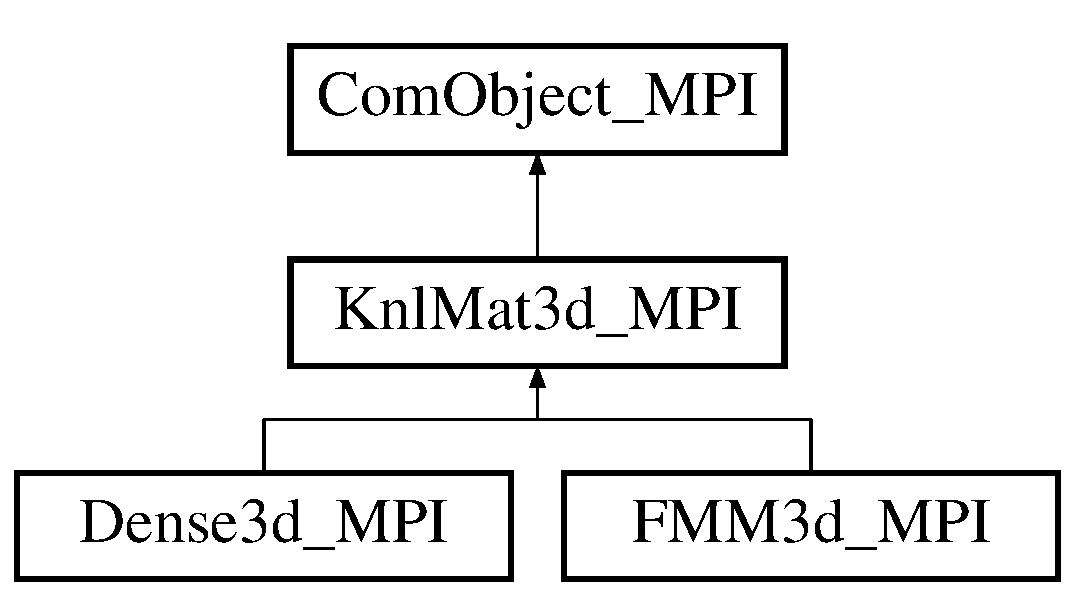
\includegraphics[height=3cm]{classKnlMat3d__MPI}
\end{center}
\end{figure}


\subsection{Detailed Description}
Knl\-Mat3d\_\-MPI is an mpi version of Knl\-Mat3d - storing kernel and matrix information for 3d. Knl\-Mat3d\_\-MPI builds upon {\bf Com\-Object\_\-MPI}{\rm (p.\,\pageref{classComObject__MPI})} - for use with FMM\_\-3d\_\-MPI or {\bf Dense3d\_\-MPI}{\rm (p.\,\pageref{classDense3d__MPI})} by including virtual functions for {\bf setup()}{\rm (p.\,\pageref{classKnlMat3d__MPI_98f7aa1beebfd344710d076d3d6413a2_98f7aa1beebfd344710d076d3d6413a2})} and evaluate(...) as well as accesses to information such as source positions, target values, etc. 



Definition at line 29 of file knlmat3d\_\-mpi.hpp.\subsection*{Public Member Functions}
\begin{CompactItemize}
\item 
{\bf Knl\-Mat3d\_\-MPI} (const string \&p)
\item 
virtual {\bf $\sim$Knl\-Mat3d\_\-MPI} ()
\item 
Vec \& {\bf src\-Pos} ()
\item 
Vec \& {\bf src\-Nor} ()
\item 
Vec \& {\bf trg\-Pos} ()
\item 
{\bf Kernel3d\_\-MPI} \& {\bf knl} ()
\item 
virtual int {\bf setup} ()=0
\item 
virtual int {\bf evaluate} (Vec src\-Den, Vec trg\-Val)=0
\item 
int {\bf dim} ()
\item 
int {\bf src\-DOF} ()
\item 
int {\bf trg\-DOF} ()
\item 
int {\bf proc\-Lcl\-Num} (Vec pos)
\item 
int {\bf proc\-Glb\-Num} (Vec pos)
\item 
void {\bf proc\-Lcl\-Ran} (Vec pos, int \&beg, int \&end)
\end{CompactItemize}
\subsection*{Protected Attributes}
\begin{CompactItemize}
\item 
Vec {\bf \_\-src\-Pos}
\item 
Vec {\bf \_\-src\-Nor}
\item 
Vec {\bf \_\-trg\-Pos}
\item 
{\bf Kernel3d\_\-MPI} {\bf \_\-knl}
\end{CompactItemize}


\subsection{Constructor \& Destructor Documentation}
\index{KnlMat3d_MPI@{Knl\-Mat3d\_\-MPI}!KnlMat3d_MPI@{KnlMat3d\_\-MPI}}
\index{KnlMat3d_MPI@{KnlMat3d\_\-MPI}!KnlMat3d_MPI@{Knl\-Mat3d\_\-MPI}}
\subsubsection{\setlength{\rightskip}{0pt plus 5cm}Knl\-Mat3d\_\-MPI::Knl\-Mat3d\_\-MPI (const string \& {\em p})\hspace{0.3cm}{\tt  [inline]}}\label{classKnlMat3d__MPI_c66fe250a6e3b06ad193f069d8153419_c66fe250a6e3b06ad193f069d8153419}


Construct the Knl\-Mat3d\_\-MPI object, using a string, which is passed to Com\-Object. For example, \char`\"{}fmm3d\_\-\char`\"{} for fmm3d. \_\-src\-Pos, \_\-src\-Nor, and \_\-trg\-Pos are set to NULL 

Definition at line 44 of file knlmat3d\_\-mpi.hpp.

\footnotesize\begin{verbatim}44                                : 
45          ComObject_MPI(p), _srcPos(NULL), _srcNor(NULL), _trgPos(NULL) {;}
\end{verbatim}\normalsize 


\index{KnlMat3d_MPI@{Knl\-Mat3d\_\-MPI}!~KnlMat3d_MPI@{$\sim$KnlMat3d\_\-MPI}}
\index{~KnlMat3d_MPI@{$\sim$KnlMat3d\_\-MPI}!KnlMat3d_MPI@{Knl\-Mat3d\_\-MPI}}
\subsubsection{\setlength{\rightskip}{0pt plus 5cm}virtual Knl\-Mat3d\_\-MPI::$\sim$Knl\-Mat3d\_\-MPI ()\hspace{0.3cm}{\tt  [inline, virtual]}}\label{classKnlMat3d__MPI_79335cbcac8d5b9babe0b4a6394e2caa_79335cbcac8d5b9babe0b4a6394e2caa}


destructor - calls $\sim$Com\-Object() 

Definition at line 47 of file knlmat3d\_\-mpi.hpp.

\footnotesize\begin{verbatim}47 { }
\end{verbatim}\normalsize 




\subsection{Member Function Documentation}
\index{KnlMat3d_MPI@{Knl\-Mat3d\_\-MPI}!dim@{dim}}
\index{dim@{dim}!KnlMat3d_MPI@{Knl\-Mat3d\_\-MPI}}
\subsubsection{\setlength{\rightskip}{0pt plus 5cm}int Knl\-Mat3d\_\-MPI::dim ()\hspace{0.3cm}{\tt  [inline]}}\label{classKnlMat3d__MPI_e3f9953141ca7d7525b58c0ff1ef6b1f_e3f9953141ca7d7525b58c0ff1ef6b1f}


Return dimension of the problem. Set to 3 

Definition at line 65 of file knlmat3d\_\-mpi.hpp.

Referenced by FMM3d\_\-MPI::check(), FMM3d\_\-MPI::ctb\-Src\-Exa\-Nor(), Dense3d\_\-MPI::evaluate(), FMM3d\_\-MPI::eva\-Trg\-Exa\-Pos(), proc\-Glb\-Num(), proc\-Lcl\-Num(), proc\-Lcl\-Ran(), FMM3d\_\-MPI::usr\-Src\-Exa\-Nor(), and FMM3d\_\-MPI::usr\-Src\-Exa\-Pos().

\footnotesize\begin{verbatim}65 { return 3; }
\end{verbatim}\normalsize 


\index{KnlMat3d_MPI@{Knl\-Mat3d\_\-MPI}!evaluate@{evaluate}}
\index{evaluate@{evaluate}!KnlMat3d_MPI@{Knl\-Mat3d\_\-MPI}}
\subsubsection{\setlength{\rightskip}{0pt plus 5cm}virtual int Knl\-Mat3d\_\-MPI::evaluate (Vec {\em src\-Den}, Vec {\em trg\-Val})\hspace{0.3cm}{\tt  [pure virtual]}}\label{classKnlMat3d__MPI_abf7f0a466fbc47db0804a35093c819f_abf7f0a466fbc47db0804a35093c819f}


virtual evaluation function. takes source densities and evaluates target values depending on kernel 

Implemented in {\bf Dense3d\_\-MPI} {\rm (p.\,\pageref{classDense3d__MPI_b6d6d5d529463497e5bed037a921cfc2_b6d6d5d529463497e5bed037a921cfc2})}, and {\bf FMM3d\_\-MPI} {\rm (p.\,\pageref{classFMM3d__MPI_8db45026f69e4b2b504f0c491c170d7d_8db45026f69e4b2b504f0c491c170d7d})}.\index{KnlMat3d_MPI@{Knl\-Mat3d\_\-MPI}!knl@{knl}}
\index{knl@{knl}!KnlMat3d_MPI@{Knl\-Mat3d\_\-MPI}}
\subsubsection{\setlength{\rightskip}{0pt plus 5cm}{\bf Kernel3d\_\-MPI}\& Knl\-Mat3d\_\-MPI::knl ()\hspace{0.3cm}{\tt  [inline]}}\label{classKnlMat3d__MPI_d01911fc223ab4bc9604db12f942194e_d01911fc223ab4bc9604db12f942194e}




Definition at line 56 of file knlmat3d\_\-mpi.hpp.

References \_\-knl.

Referenced by main().

\footnotesize\begin{verbatim}56 { return _knl; }
\end{verbatim}\normalsize 


\index{KnlMat3d_MPI@{Knl\-Mat3d\_\-MPI}!procGlbNum@{procGlbNum}}
\index{procGlbNum@{procGlbNum}!KnlMat3d_MPI@{Knl\-Mat3d\_\-MPI}}
\subsubsection{\setlength{\rightskip}{0pt plus 5cm}int Knl\-Mat3d\_\-MPI::proc\-Glb\-Num (Vec {\em pos})\hspace{0.3cm}{\tt  [inline]}}\label{classKnlMat3d__MPI_47cb2afea618c56a5cc6e05f4034a806_47cb2afea618c56a5cc6e05f4034a806}


global number of positions for this processor 

Definition at line 74 of file knlmat3d\_\-mpi.hpp.

References dim().

Referenced by FMM3d\_\-MPI::evaluate(), and Dense3d\_\-MPI::evaluate().

\footnotesize\begin{verbatim}74 { int tmp; VecGetSize(     pos, &tmp); return tmp/dim(); }
\end{verbatim}\normalsize 


\index{KnlMat3d_MPI@{Knl\-Mat3d\_\-MPI}!procLclNum@{procLclNum}}
\index{procLclNum@{procLclNum}!KnlMat3d_MPI@{Knl\-Mat3d\_\-MPI}}
\subsubsection{\setlength{\rightskip}{0pt plus 5cm}int Knl\-Mat3d\_\-MPI::proc\-Lcl\-Num (Vec {\em pos})\hspace{0.3cm}{\tt  [inline]}}\label{classKnlMat3d__MPI_21f80b863e1376ff6648d882fdabd08e_21f80b863e1376ff6648d882fdabd08e}


local number of positions for this processor 

Definition at line 72 of file knlmat3d\_\-mpi.hpp.

References dim().

Referenced by FMM3d\_\-MPI::check(), and Dense3d\_\-MPI::evaluate().

\footnotesize\begin{verbatim}72 { int tmp; VecGetLocalSize(pos, &tmp); return tmp/dim(); }
\end{verbatim}\normalsize 


\index{KnlMat3d_MPI@{Knl\-Mat3d\_\-MPI}!procLclRan@{procLclRan}}
\index{procLclRan@{procLclRan}!KnlMat3d_MPI@{Knl\-Mat3d\_\-MPI}}
\subsubsection{\setlength{\rightskip}{0pt plus 5cm}void Knl\-Mat3d\_\-MPI::proc\-Lcl\-Ran (Vec {\em pos}, int \& {\em beg}, int \& {\em end})\hspace{0.3cm}{\tt  [inline]}}\label{classKnlMat3d__MPI_c77ddf71aecd48cd8a8ed887d5bcd834_c77ddf71aecd48cd8a8ed887d5bcd834}


processor Local Range. for vector pos, return the beginning and end range positions for which the local processor is responsible 

Definition at line 77 of file knlmat3d\_\-mpi.hpp.

References dim().

\footnotesize\begin{verbatim}77 { VecGetOwnershipRange(pos, &beg, &end); beg=beg/dim(); end=end/dim(); }
\end{verbatim}\normalsize 


\index{KnlMat3d_MPI@{Knl\-Mat3d\_\-MPI}!setup@{setup}}
\index{setup@{setup}!KnlMat3d_MPI@{Knl\-Mat3d\_\-MPI}}
\subsubsection{\setlength{\rightskip}{0pt plus 5cm}virtual int Knl\-Mat3d\_\-MPI::setup ()\hspace{0.3cm}{\tt  [pure virtual]}}\label{classKnlMat3d__MPI_98f7aa1beebfd344710d076d3d6413a2_98f7aa1beebfd344710d076d3d6413a2}


virtual setup function 

Implemented in {\bf Dense3d\_\-MPI} {\rm (p.\,\pageref{classDense3d__MPI_415266b005d267e801176f27c0434a50_415266b005d267e801176f27c0434a50})}, and {\bf FMM3d\_\-MPI} {\rm (p.\,\pageref{classFMM3d__MPI_415266b005d267e801176f27c0434a50_415266b005d267e801176f27c0434a50})}.\index{KnlMat3d_MPI@{Knl\-Mat3d\_\-MPI}!srcDOF@{srcDOF}}
\index{srcDOF@{srcDOF}!KnlMat3d_MPI@{Knl\-Mat3d\_\-MPI}}
\subsubsection{\setlength{\rightskip}{0pt plus 5cm}int Knl\-Mat3d\_\-MPI::src\-DOF ()\hspace{0.3cm}{\tt  [inline]}}\label{classKnlMat3d__MPI_6b422ba557bb24eff82ac7125e206568_6b422ba557bb24eff82ac7125e206568}


Return source degree of freedom: \_\-knl.src\-DOF() - see {\bf kernel3d\_\-mpi.hpp}{\rm (p.\,\pageref{kernel3d__mpi_8hpp})} 

Definition at line 67 of file knlmat3d\_\-mpi.hpp.

References \_\-knl, and Kernel3d\_\-MPI::src\-DOF().

Referenced by FMM3d\_\-MPI::check(), FMM3d\_\-MPI::ctb\-Src\-Exa\-Den(), FMM3d\_\-MPI::evaluate(), Dense3d\_\-MPI::evaluate(), and FMM3d\_\-MPI::usr\-Src\-Exa\-Den().

\footnotesize\begin{verbatim}67 { return _knl.srcDOF(); }
\end{verbatim}\normalsize 


\index{KnlMat3d_MPI@{Knl\-Mat3d\_\-MPI}!srcNor@{srcNor}}
\index{srcNor@{srcNor}!KnlMat3d_MPI@{Knl\-Mat3d\_\-MPI}}
\subsubsection{\setlength{\rightskip}{0pt plus 5cm}Vec\& Knl\-Mat3d\_\-MPI::src\-Nor ()\hspace{0.3cm}{\tt  [inline]}}\label{classKnlMat3d__MPI_bba2c6a917421951f1fbe8f69b9a135b_bba2c6a917421951f1fbe8f69b9a135b}


Return source normals 

Definition at line 52 of file knlmat3d\_\-mpi.hpp.

References \_\-src\-Nor.

Referenced by main().

\footnotesize\begin{verbatim}52 { return _srcNor; }
\end{verbatim}\normalsize 


\index{KnlMat3d_MPI@{Knl\-Mat3d\_\-MPI}!srcPos@{srcPos}}
\index{srcPos@{srcPos}!KnlMat3d_MPI@{Knl\-Mat3d\_\-MPI}}
\subsubsection{\setlength{\rightskip}{0pt plus 5cm}Vec\& Knl\-Mat3d\_\-MPI::src\-Pos ()\hspace{0.3cm}{\tt  [inline]}}\label{classKnlMat3d__MPI_caa1dae06f56964efa0f778b696dce61_caa1dae06f56964efa0f778b696dce61}


Return source positions 

Definition at line 50 of file knlmat3d\_\-mpi.hpp.

References \_\-src\-Pos.

Referenced by main().

\footnotesize\begin{verbatim}50 { return _srcPos; }
\end{verbatim}\normalsize 


\index{KnlMat3d_MPI@{Knl\-Mat3d\_\-MPI}!trgDOF@{trgDOF}}
\index{trgDOF@{trgDOF}!KnlMat3d_MPI@{Knl\-Mat3d\_\-MPI}}
\subsubsection{\setlength{\rightskip}{0pt plus 5cm}int Knl\-Mat3d\_\-MPI::trg\-DOF ()\hspace{0.3cm}{\tt  [inline]}}\label{classKnlMat3d__MPI_ea43c1f768349e86110e4e2d06e38d10_ea43c1f768349e86110e4e2d06e38d10}


Return target degree of freedom: \_\-knl.trg\-DOF() - see {\bf kernel3d\_\-mpi.hpp}{\rm (p.\,\pageref{kernel3d__mpi_8hpp})} 

Definition at line 69 of file knlmat3d\_\-mpi.hpp.

References \_\-knl, and Kernel3d\_\-MPI::trg\-DOF().

Referenced by FMM3d\_\-MPI::check(), FMM3d\_\-MPI::evaluate(), Dense3d\_\-MPI::evaluate(), and FMM3d\_\-MPI::eva\-Trg\-Exa\-Val().

\footnotesize\begin{verbatim}69 { return _knl.trgDOF(); }
\end{verbatim}\normalsize 


\index{KnlMat3d_MPI@{Knl\-Mat3d\_\-MPI}!trgPos@{trgPos}}
\index{trgPos@{trgPos}!KnlMat3d_MPI@{Knl\-Mat3d\_\-MPI}}
\subsubsection{\setlength{\rightskip}{0pt plus 5cm}Vec\& Knl\-Mat3d\_\-MPI::trg\-Pos ()\hspace{0.3cm}{\tt  [inline]}}\label{classKnlMat3d__MPI_7dc770563c182703b1986abb06c6dbbd_7dc770563c182703b1986abb06c6dbbd}


Return target positions 

Definition at line 54 of file knlmat3d\_\-mpi.hpp.

References \_\-trg\-Pos.

Referenced by main().

\footnotesize\begin{verbatim}54 { return _trgPos; }
\end{verbatim}\normalsize 




\subsection{Member Data Documentation}
\index{KnlMat3d_MPI@{Knl\-Mat3d\_\-MPI}!_knl@{\_\-knl}}
\index{_knl@{\_\-knl}!KnlMat3d_MPI@{Knl\-Mat3d\_\-MPI}}
\subsubsection{\setlength{\rightskip}{0pt plus 5cm}{\bf Kernel3d\_\-MPI} {\bf Knl\-Mat3d\_\-MPI::\_\-knl}\hspace{0.3cm}{\tt  [protected]}}\label{classKnlMat3d__MPI_cb56a4f532a89bc1a51ee17c2434a106_cb56a4f532a89bc1a51ee17c2434a106}


the kernel being used, defined in {\bf kernel3d\_\-mpi.hpp}{\rm (p.\,\pageref{kernel3d__mpi_8hpp})} - defines kernel type and coefficients 

Definition at line 40 of file knlmat3d\_\-mpi.hpp.

Referenced by Dense3d\_\-MPI::evaluate(), knl(), FMM3d\_\-MPI::setup(), src\-DOF(), FMM3d\_\-MPI::Src\-Equ2Trg\-Chk\_\-dgemv(), and trg\-DOF().\index{KnlMat3d_MPI@{Knl\-Mat3d\_\-MPI}!_srcNor@{\_\-srcNor}}
\index{_srcNor@{\_\-srcNor}!KnlMat3d_MPI@{Knl\-Mat3d\_\-MPI}}
\subsubsection{\setlength{\rightskip}{0pt plus 5cm}Vec {\bf Knl\-Mat3d\_\-MPI::\_\-src\-Nor}\hspace{0.3cm}{\tt  [protected]}}\label{classKnlMat3d__MPI_bbeec6db21041e1b277f4755f21047dd_bbeec6db21041e1b277f4755f21047dd}


Source normals 

Definition at line 36 of file knlmat3d\_\-mpi.hpp.

Referenced by Dense3d\_\-MPI::evaluate(), FMM3d\_\-MPI::setup(), Dense3d\_\-MPI::setup(), and src\-Nor().\index{KnlMat3d_MPI@{Knl\-Mat3d\_\-MPI}!_srcPos@{\_\-srcPos}}
\index{_srcPos@{\_\-srcPos}!KnlMat3d_MPI@{Knl\-Mat3d\_\-MPI}}
\subsubsection{\setlength{\rightskip}{0pt plus 5cm}Vec {\bf Knl\-Mat3d\_\-MPI::\_\-src\-Pos}\hspace{0.3cm}{\tt  [protected]}}\label{classKnlMat3d__MPI_f66b814fdf8eb17df56ff5ff27a368da_f66b814fdf8eb17df56ff5ff27a368da}


Source positions 

Definition at line 34 of file knlmat3d\_\-mpi.hpp.

Referenced by FMM3d\_\-MPI::check(), FMM3d\_\-MPI::evaluate(), Dense3d\_\-MPI::evaluate(), FMM3d\_\-MPI::setup(), Dense3d\_\-MPI::setup(), and src\-Pos().\index{KnlMat3d_MPI@{Knl\-Mat3d\_\-MPI}!_trgPos@{\_\-trgPos}}
\index{_trgPos@{\_\-trgPos}!KnlMat3d_MPI@{Knl\-Mat3d\_\-MPI}}
\subsubsection{\setlength{\rightskip}{0pt plus 5cm}Vec {\bf Knl\-Mat3d\_\-MPI::\_\-trg\-Pos}\hspace{0.3cm}{\tt  [protected]}}\label{classKnlMat3d__MPI_a1b44c7c6fd0a38be167c34537b1a508_a1b44c7c6fd0a38be167c34537b1a508}


Target positions 

Definition at line 38 of file knlmat3d\_\-mpi.hpp.

Referenced by FMM3d\_\-MPI::check(), FMM3d\_\-MPI::evaluate(), Dense3d\_\-MPI::evaluate(), FMM3d\_\-MPI::setup(), Dense3d\_\-MPI::setup(), and trg\-Pos().

The documentation for this class was generated from the following file:\begin{CompactItemize}
\item 
fmm3d\_\-mpi/{\bf knlmat3d\_\-mpi.hpp}\end{CompactItemize}

\section{Let3d\_\-MPI Class Reference}
\label{classLet3d__MPI}\index{Let3d_MPI@{Let3d\_\-MPI}}
{\tt \#include $<$let3d\_\-mpi.hpp$>$}

Inheritance diagram for Let3d\_\-MPI::\begin{figure}[H]
\begin{center}
\leavevmode
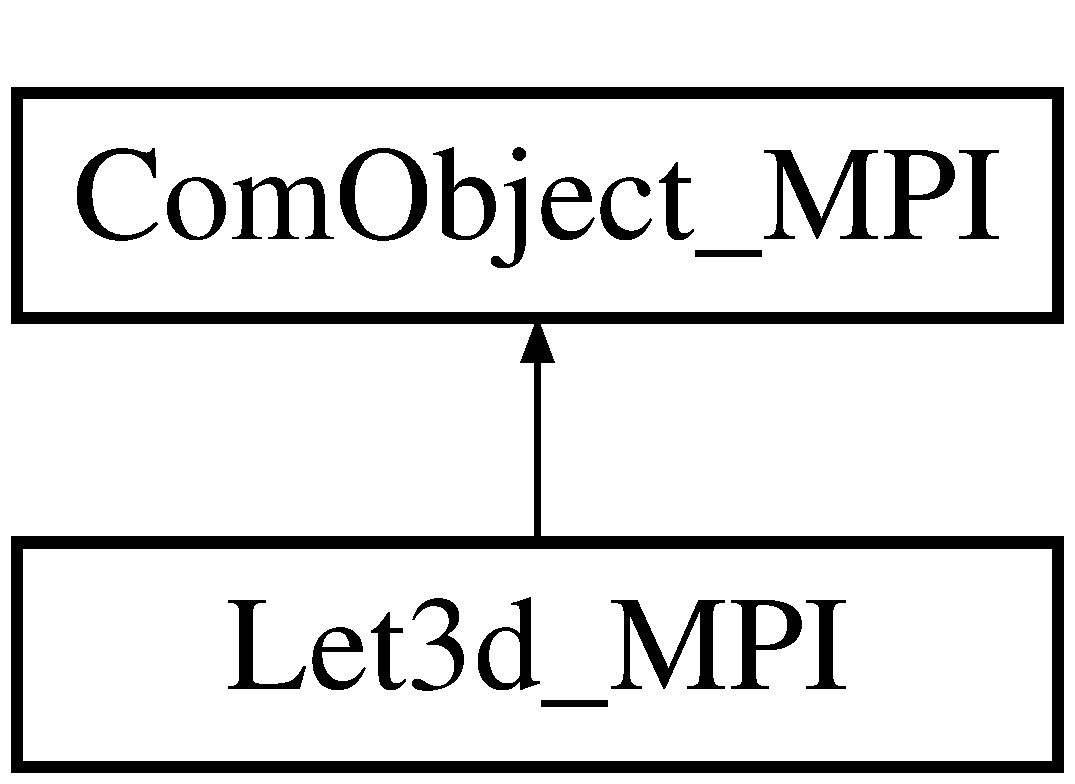
\includegraphics[height=2cm]{classLet3d__MPI}
\end{center}
\end{figure}


\subsection{Detailed Description}
LET = Local Essential Tree. See detailed description for more information. 

The LET is a global tree subset that a processor needs to evaluate the interaction on particles which belong to itself (owns). That is, it is a unique identifier: a set of points and its bounding box. To this extent, for a box/node B, the information from B's lists are needed. Specifically, the U, V, W and X lists are used for computation. More information is in the descriptiptions of \_\-Unodes, etc. and the papers. For a processor P, P's LET contains the boxes which P \char`\"{}owns\char`\"{} and boxes in the U,V,W and X lists of these boxes. For a box, B, owned by P, P is a contributor of B. If B is in the U,V,W or X lists of a box P owns, P is a user of B. For more information, see \char`\"{}A New Parallel Kernel-Independent Fast Multipole Method\char`\"{} by Ying, Biros, Zorin and Langston. 



Definition at line 51 of file let3d\_\-mpi.hpp.\subsection*{Public Member Functions}
\begin{CompactItemize}
\item 
{\bf Let3d\_\-MPI} (const string \&p)
\item 
{\bf $\sim$Let3d\_\-MPI} ()
\item 
Vec \& {\bf src\-Pos} ()
\item 
Vec \& {\bf trg\-Pos} ()
\item 
Point3 \& {\bf ctr} ()
\item 
int \& {\bf root\-Level} ()
\item 
double {\bf radius} ()
\item 
int \& {\bf pts\-Max} ()
\item 
int \& {\bf max\-Level} ()
\item 
int {\bf setup} ()
\item 
int {\bf print} ()
\item 
int {\bf src\-Data} ()
\item 
int {\bf trg\-Data} ()
\item 
int {\bf cal\-Glb\-Node\-Lists} (int g\-Node\-Idx)
\item 
int {\bf dwn\-Order\-Collect} (vector$<$ int $>$ \&)
\item 
int {\bf upw\-Order\-Collect} (vector$<$ int $>$ \&)
\item 
vector$<$ {\bf Node} $>$ \& {\bf node\-Vec} ()
\item 
{\bf Node} \& {\bf node} (int g\-Node\-Idx)
\item 
bool {\bf root} (int g\-Node\-Idx)
\item 
bool {\bf terminal} (int g\-Node\-Idx)
\item 
int {\bf parent} (int g\-Node\-Idx)
\item 
int {\bf child} (int g\-Node\-Idx, const Index3 \&Idx)
\item 
Index3 {\bf path2Node} (int g\-Node\-Idx)
\item 
int {\bf depth} (int g\-Node\-Idx)
\item 
Point3 {\bf center} (int g\-Node\-Idx)
\item 
double {\bf radius} (int g\-Node\-Idx)
\item 
int \& {\bf glb\-Glb\-Src\-Node\-Cnt} ()
\item 
int \& {\bf glb\-Glb\-Src\-Exa\-Cnt} ()
\item 
int \& {\bf lcl\-Glb\-Src\-Node\-Cnt} ()
\item 
int \& {\bf lcl\-Glb\-Src\-Exa\-Cnt} ()
\item 
int \& {\bf ctb\-Src\-Node\-Cnt} ()
\item 
int \& {\bf ctb\-Src\-Exa\-Cnt} ()
\item 
vector$<$ int $>$ \& {\bf ctb2Glb\-Src\-Node\-Map} ()
\item 
vector$<$ int $>$ \& {\bf ctb2Glb\-Src\-Exa\-Map} ()
\item 
int \& {\bf eva\-Trg\-Node\-Cnt} ()
\item 
int \& {\bf eva\-Trg\-Exa\-Cnt} ()
\item 
int \& {\bf usr\-Src\-Node\-Cnt} ()
\item 
int \& {\bf usr\-Src\-Exa\-Cnt} ()
\item 
vector$<$ int $>$ \& {\bf usr2Glb\-Src\-Node\-Map} ()
\item 
vector$<$ int $>$ \& {\bf usr2Glb\-Src\-Exa\-Map} ()
\item 
int {\bf find\-Glb\-Node} (int depth, const Index3 \&path2Node)
\item 
bool {\bf adjacent} (int me, int you)
\item 
int {\bf dim} () const 
\item 
int {\bf proc\-Lcl\-Num} (Vec pos)
\item 
int {\bf proc\-Glb\-Num} (Vec pos)
\item 
void {\bf proc\-Lcl\-Ran} (Vec pos, int \&beg, int \&end)
\end{CompactItemize}
\subsection*{Protected Attributes}
\begin{CompactItemize}
\item 
Vec {\bf \_\-src\-Pos}
\item 
Vec {\bf \_\-trg\-Pos}
\item 
Point3 {\bf \_\-ctr}
\item 
int {\bf \_\-root\-Level}
\item 
int {\bf \_\-pts\-Max}
\item 
int {\bf \_\-max\-Level}
\item 
vector$<$ {\bf Node} $>$ {\bf \_\-node\-Vec}
\item 
int {\bf \_\-glb\-Glb\-Src\-Node\-Cnt}
\item 
int {\bf \_\-glb\-Glb\-Src\-Exa\-Cnt}
\item 
int {\bf \_\-lcl\-Glb\-Src\-Node\-Cnt}
\item 
int {\bf \_\-lcl\-Glb\-Src\-Exa\-Cnt}
\item 
int {\bf \_\-ctb\-Src\-Node\-Cnt}
\item 
int {\bf \_\-ctb\-Src\-Exa\-Cnt}
\item 
vector$<$ int $>$ {\bf \_\-ctb2Glb\-Src\-Node\-Map}
\item 
vector$<$ int $>$ {\bf \_\-ctb2Glb\-Src\-Exa\-Map}
\item 
int {\bf \_\-eva\-Trg\-Node\-Cnt}
\item 
int {\bf \_\-eva\-Trg\-Exa\-Cnt}
\item 
int {\bf \_\-usr\-Src\-Node\-Cnt}
\item 
int {\bf \_\-usr\-Src\-Exa\-Cnt}
\item 
vector$<$ int $>$ {\bf \_\-usr2Glb\-Src\-Node\-Map}
\item 
vector$<$ int $>$ {\bf \_\-usr2Glb\-Src\-Exa\-Map}
\end{CompactItemize}
\subsection*{Classes}
\begin{CompactItemize}
\item 
class {\bf Node}
\begin{CompactList}\small\item\em The {\bf Node}{\rm (p.\,\pageref{classLet3d__MPI_1_1Node})} class stores information for a node or box in the octree. See for more detailed information. \item\end{CompactList}\item 
class {\bf Node\-Ext}
\begin{CompactList}\small\item\em {\bf Node\-Ext}{\rm (p.\,\pageref{classLet3d__MPI_1_1NodeExt})} stores information for a node such U, v, w, and X-lists as well as indices for contributor, evaluator and user nodes. \item\end{CompactList}\end{CompactItemize}


\subsection{Constructor \& Destructor Documentation}
\index{Let3d_MPI@{Let3d\_\-MPI}!Let3d_MPI@{Let3d\_\-MPI}}
\index{Let3d_MPI@{Let3d\_\-MPI}!Let3d_MPI@{Let3d\_\-MPI}}
\subsubsection{\setlength{\rightskip}{0pt plus 5cm}Let3d\_\-MPI::Let3d\_\-MPI (const string \& {\em p})}\label{classLet3d__MPI_0b17f9aae24c3678a5111a92d1b9ffb2_0b17f9aae24c3678a5111a92d1b9ffb2}


Construct Let3D\_\-MPI with string for Com\-Object 

Definition at line 29 of file let3d\_\-mpi.cpp.

\footnotesize\begin{verbatim}29                                    :
30   ComObject_MPI(p), _srcPos(NULL), _trgPos(NULL), _ctr(0.0), _rootLevel(0),
31   _ptsMax(150), _maxLevel(10)
32 {
33 }

\end{verbatim}\normalsize 


\index{Let3d_MPI@{Let3d\_\-MPI}!~Let3d_MPI@{$\sim$Let3d\_\-MPI}}
\index{~Let3d_MPI@{$\sim$Let3d\_\-MPI}!Let3d_MPI@{Let3d\_\-MPI}}
\subsubsection{\setlength{\rightskip}{0pt plus 5cm}Let3d\_\-MPI::$\sim$Let3d\_\-MPI ()}\label{classLet3d__MPI_ac2ccc7a2461eab6f090002aec2c87f9_ac2ccc7a2461eab6f090002aec2c87f9}




Definition at line 35 of file let3d\_\-mpi.cpp.

\footnotesize\begin{verbatim}36 {
37 }
\end{verbatim}\normalsize 




\subsection{Member Function Documentation}
\index{Let3d_MPI@{Let3d\_\-MPI}!adjacent@{adjacent}}
\index{adjacent@{adjacent}!Let3d_MPI@{Let3d\_\-MPI}}
\subsubsection{\setlength{\rightskip}{0pt plus 5cm}bool Let3d\_\-MPI::adjacent (int {\em me}, int {\em you})}\label{classLet3d__MPI_bd4b53389da8d68ee7218abbe006c28d_bd4b53389da8d68ee7218abbe006c28d}


Check if node\-Vec[me] is adjacent to node\-Vec[you] 

Definition at line 841 of file let3d\_\-mpi.cpp.

References \_\-\_\-FUNCT\_\-\_\-, depth(), path2Node(), and radius().

\footnotesize\begin{verbatim}842 {
843   int maxDepth = max(depth(me),depth(you)); /* Which node is at a greater depth */
844   Index3 one(1); /* = (1,1,1) */
845   /* Construct the center for both nodes */
846   Index3 meCtr(  (2*path2Node(me)+one) * pow2(maxDepth - depth(me))  );
847   Index3 youCtr(  (2*path2Node(you)+one) * pow2(maxDepth - depth(you))  );
848   /* construct radii for both nodes */
849   int meRad = pow2(maxDepth - depth(me));
850   int youRad = pow2(maxDepth - depth(you));
851   /* absolute value of difference of centers */
852   Index3 dif( abs(meCtr-youCtr) );
853   /* sum of radii */
854   int radius  = meRad + youRad;
855   /* if the abs. value of difference of centers is less than the sum of the radii
856         * AND the infinity norm equals the sum of the radii, then the two nodes
857         * are not too far away AND at least one edge touches */
858   return
859          ( dif <= Index3(radius) ) && //not too far
860          ( dif.linfty() == radius ); //at least one edge touch
861 }
\end{verbatim}\normalsize 


\index{Let3d_MPI@{Let3d\_\-MPI}!calGlbNodeLists@{calGlbNodeLists}}
\index{calGlbNodeLists@{calGlbNodeLists}!Let3d_MPI@{Let3d\_\-MPI}}
\subsubsection{\setlength{\rightskip}{0pt plus 5cm}int Let3d\_\-MPI::cal\-Glb\-Node\-Lists (int {\em g\-Node\-Idx})}\label{classLet3d__MPI_d1ba4ee8bb99cce06a89eb96cb9ddf8c_d1ba4ee8bb99cce06a89eb96cb9ddf8c}


Build U,V,W, and X lists for a specific node, indicated by an integer location in the global node index. 

Definition at line 635 of file let3d\_\-mpi.cpp.

\footnotesize\begin{verbatim}636 {
637   //begin
638   /* We use sets here since the values will be unnecessary to keep associated with the keys.
639         * Can also use a C++ map, but it is unnecessary here to maintain unique key/value pairs
640         * See let3d_mpi.hpp for descriptions of what U,B,W, and X lsists are. */
641   set<int> Uset, Vset, Wset, Xset;  
642   int curgNodeIdx = gNodeIdx;
643   /* Make sure current node is not the root as the root has no ancestors */
644   if(root(curgNodeIdx)==false) {
645          /* get parent of node we're interested in */
646          int pargNodeIdx = parent(curgNodeIdx);
647          Index3 minIdx(0); /* = (0,0,0) */
648          Index3 maxIdx(pow2(depth(curgNodeIdx))); /* = (2^d, 2^d, 2^d) */
649          
650          /* Try several different paths.  Here we are looking for paths which
651           * will lead to children of neighbors of the parent of the current node
652           * in order to build U,V,W, and X lists */
653          for(int i=-2; i<4; i++) {
654                 for(int j=-2; j<4; j++) {
655                   for(int k=-2; k<4; k++) {
656                          /* New Path to try */
657                          Index3 tryPath2Node( 2*path2Node(pargNodeIdx) + Index3(i,j,k) );
658                          /* Verify new path does not exceed a maximu index and is greater than (0,0,0) and is not equal to current node's path */
659                          if(tryPath2Node >= minIdx && tryPath2Node <  maxIdx && tryPath2Node != path2Node(curgNodeIdx)) {
660                                 /* Look for the children of the neighbors of the current node's parent */
661                                 int resgNodeIdx = findGlbNode(depth(curgNodeIdx), tryPath2Node);
662                                 /* adj = true if nodes have at least one edge touching */
663                                 bool adj = adjacent(resgNodeIdx, curgNodeIdx);
664                                 /* When test node is higher in the tree than current node */
665                                 if( depth(resgNodeIdx)<depth(curgNodeIdx) ) {
666                                   /* If adjacent and current node is a leaf, put test node in the Uset if the current node is a leaf */
667                                   if(adj){
668                                          if(terminal(curgNodeIdx)){ /* need to test if res a leaf?? HARPER */
669                                                 Uset.insert(resgNodeIdx);
670                                          }
671                                          else {;} /* non-leaves do not have U-lists */
672                                   }
673                                   else{
674                                          /* The nodes are not adjacent, but resgNodeIdx is still a child of the current node's parent's neighbors.
675                                           * Hence, the current node's parent is adjacent to resgNodeIdx.  IN general. the current node is in the
676                                           * W-list of resgNodeIdx */
677                                          Xset.insert(resgNodeIdx);
678                                   }
679                                 } /* End of "if depth(res) < depth(current) " */
680                                 
681                                 /* Current node and test node at same depth */
682                                 if( depth(resgNodeIdx)==depth(curgNodeIdx) ) {
683                                   /* Two nodes at same depth not adjacent */
684                                   if(!adj) {
685                                          Index3 bb(path2Node(resgNodeIdx)-path2Node(curgNodeIdx));
686                                          /* Verify that no single component of the two paths exceed a limit */
687                                          assert( bb.linfty()<=3 );
688                                          /* resgNodeIdx is a child of the neighbor's of the currentr node's parents and not-adjacent to current node.
689                                           * Hence, it is in the V-list */
690                                          Vset.insert(resgNodeIdx);
691                                   }
692                                   /* nodes at same depth and are adjacent, so resgNodeIdx could be in U OR W lists */
693                                   else {
694                                          if(terminal(curgNodeIdx)) {
695                                                 /* queue:  elements added/pushed to the back and removed/popped from the front */ 
696                                                 queue<int> rest;
697                                                 /* push resgNodeIdx into the queue */
698                                                 rest.push(resgNodeIdx);
699                                                 while(rest.empty()==false) {
700                                                   int fntgNodeIdx = rest.front(); rest.pop(); /* Set front temp node index and pop the list */
701                                                   /* If the current node and temp node are not adjacent, temp node is in W-list of current node */
702                                                   if(adjacent(fntgNodeIdx, curgNodeIdx)==false) {
703                                                          Wset.insert( fntgNodeIdx );
704                                                   }
705                                                   /* Current node and temp node ARE adjacent */
706                                                   else {
707                                                          /* If temp node is a leaf, it is in current node's U-list */
708                                                          if(terminal(fntgNodeIdx)) {
709                                                                 Uset.insert(fntgNodeIdx);
710                                                          }
711                                                          /* If temp node is not a leaf, then one of its descendants may be a leaf in the U or W lists of current node
712                                                          * So, we push those into the queue
713                                                          */
714                                                          else { 
715                                                                 for(int a=0; a<2; a++) {
716                                                                   for(int b=0; b<2; b++) {
717                                                                          for(int c=0; c<2; c++) {
718                                                                                 rest.push( child(fntgNodeIdx, Index3(a,b,c)) );
719                                                                          }
720                                                                   }
721                                                                 }
722                                                          }
723                                                   }
724                                                 } /* End of while loop for rest queue */
725                                          } /* End of "if current node a leaf" */ 
726                                   } /* End of res and current nodes at same depth and adjacent */
727                                 } /* End of "if depth(res) == depth(current)" */
728                          } /* End of trypath */
729                   }
730                 }
731          }
732   } /* End of building sets for non-root node, curgNodeIdx */
733 
734   /* If the current node is a leaf, then it is in its own U-list */
735   if(terminal(curgNodeIdx))
736          Uset.insert(curgNodeIdx);
737 
738   /* For all sets, check to make sure all of the nodes actually have sources in them.  If not
739         * we do not need to put them in the lists.  If so, build the U,V,W, and X lists from respective sets
740         */
741   for(set<int>::iterator si=Uset.begin(); si!=Uset.end(); si++)
742          if(node(*si).tag() & LET_SRCENODE) /* Check if sources bit set for this node's tag.  Same below */
743                 node(gNodeIdx).Unodes().push_back(*si);
744   for(set<int>::iterator si=Vset.begin(); si!=Vset.end(); si++)
745          if(node(*si).tag() & LET_SRCENODE)
746                 node(gNodeIdx).Vnodes().push_back(*si);
747   for(set<int>::iterator si=Wset.begin(); si!=Wset.end(); si++)
748          if(node(*si).tag() & LET_SRCENODE)
749                 node(gNodeIdx).Wnodes().push_back(*si);
750   for(set<int>::iterator si=Xset.begin(); si!=Xset.end(); si++)
751          if(node(*si).tag() & LET_SRCENODE)
752                 node(gNodeIdx).Xnodes().push_back(*si);
753   
754   return(0);
755 }
\end{verbatim}\normalsize 


\index{Let3d_MPI@{Let3d\_\-MPI}!center@{center}}
\index{center@{center}!Let3d_MPI@{Let3d\_\-MPI}}
\subsubsection{\setlength{\rightskip}{0pt plus 5cm}Point3 Let3d\_\-MPI::center (int {\em g\-Node\-Idx})}\label{classLet3d__MPI_dff5f922c11176af18f4bfa95c138a20_dff5f922c11176af18f4bfa95c138a20}


Return the center of the box dexcribed by node\-Vec[g\-Node\-Idx] 

Definition at line 793 of file let3d\_\-mpi.cpp.

\footnotesize\begin{verbatim}794 {
795   Point3 ll( ctr() - Point3(radius()) );
796   int tmp = pow2(depth(gNodeIdx));
797   Index3 path2Node_Lcl(path2Node(gNodeIdx));
798   Point3 res;
799   for(int d=0; d<dim(); d++) {
800          res(d) = ll(d) + (2*radius()) * (path2Node_Lcl(d)+0.5) / double(tmp);
801   }
802   return res;
803 }
\end{verbatim}\normalsize 


\index{Let3d_MPI@{Let3d\_\-MPI}!child@{child}}
\index{child@{child}!Let3d_MPI@{Let3d\_\-MPI}}
\subsubsection{\setlength{\rightskip}{0pt plus 5cm}int Let3d\_\-MPI::child (int {\em g\-Node\-Idx}, const Index3 \& {\em Idx})}\label{classLet3d__MPI_b0f154b8aff8346def992423c060b862_b0f154b8aff8346def992423c060b862}


Return child of node described by g\-Node\-Idx and Idx. g\-Node\-Idx is the Node's integer descriptor in node\-Vec and Idx is a binary index from 0-$>$7, indicating which child to return. For example, child(10,(0,0,0)) returns the first child of node\-Vec[10]. child(10,(1,1,1)) returns the eighth (and last) child of node\-Vec[10]. 

Definition at line 787 of file let3d\_\-mpi.cpp.

Referenced by find\-Glb\-Node().

\footnotesize\begin{verbatim}788 {
789   assert(idx>=Index3(0) && idx<Index3(2));
790   return node(gNodeIdx).chd() + (idx(0)*4+idx(1)*2+idx(2));
791 }
\end{verbatim}\normalsize 


\index{Let3d_MPI@{Let3d\_\-MPI}!ctb2GlbSrcExaMap@{ctb2GlbSrcExaMap}}
\index{ctb2GlbSrcExaMap@{ctb2GlbSrcExaMap}!Let3d_MPI@{Let3d\_\-MPI}}
\subsubsection{\setlength{\rightskip}{0pt plus 5cm}vector$<$int$>$\& Let3d\_\-MPI::ctb2Glb\-Src\-Exa\-Map ()\hspace{0.3cm}{\tt  [inline]}}\label{classLet3d__MPI_fa7b61748f05b09067f1fc99b672099e_fa7b61748f05b09067f1fc99b672099e}


Return vector of integers describing contributor to global exact source map 

Definition at line 338 of file let3d\_\-mpi.hpp.

References \_\-ctb2Glb\-Src\-Exa\-Map.

\footnotesize\begin{verbatim}338 { return _ctb2GlbSrcExaMap; }
\end{verbatim}\normalsize 


\index{Let3d_MPI@{Let3d\_\-MPI}!ctb2GlbSrcNodeMap@{ctb2GlbSrcNodeMap}}
\index{ctb2GlbSrcNodeMap@{ctb2GlbSrcNodeMap}!Let3d_MPI@{Let3d\_\-MPI}}
\subsubsection{\setlength{\rightskip}{0pt plus 5cm}vector$<$int$>$\& Let3d\_\-MPI::ctb2Glb\-Src\-Node\-Map ()\hspace{0.3cm}{\tt  [inline]}}\label{classLet3d__MPI_2edf7ec1048f348ac03b27bc90b9d2a0_2edf7ec1048f348ac03b27bc90b9d2a0}


Return vector of integers describing contributor to global source node map 

Definition at line 336 of file let3d\_\-mpi.hpp.

References \_\-ctb2Glb\-Src\-Node\-Map.

\footnotesize\begin{verbatim}336 { return _ctb2GlbSrcNodeMap; }
\end{verbatim}\normalsize 


\index{Let3d_MPI@{Let3d\_\-MPI}!ctbSrcExaCnt@{ctbSrcExaCnt}}
\index{ctbSrcExaCnt@{ctbSrcExaCnt}!Let3d_MPI@{Let3d\_\-MPI}}
\subsubsection{\setlength{\rightskip}{0pt plus 5cm}int\& Let3d\_\-MPI::ctb\-Src\-Exa\-Cnt ()\hspace{0.3cm}{\tt  [inline]}}\label{classLet3d__MPI_ef9a057fecc402d5d641067c9a43d7af_ef9a057fecc402d5d641067c9a43d7af}


Return exact count of contributor sources 

Definition at line 334 of file let3d\_\-mpi.hpp.

References \_\-ctb\-Src\-Exa\-Cnt.

\footnotesize\begin{verbatim}334 { return _ctbSrcExaCnt; }
\end{verbatim}\normalsize 


\index{Let3d_MPI@{Let3d\_\-MPI}!ctbSrcNodeCnt@{ctbSrcNodeCnt}}
\index{ctbSrcNodeCnt@{ctbSrcNodeCnt}!Let3d_MPI@{Let3d\_\-MPI}}
\subsubsection{\setlength{\rightskip}{0pt plus 5cm}int\& Let3d\_\-MPI::ctb\-Src\-Node\-Cnt ()\hspace{0.3cm}{\tt  [inline]}}\label{classLet3d__MPI_a558f7790d074c6bf0478d3d3300e595_a558f7790d074c6bf0478d3d3300e595}


Return number of contributor source nodes 

Definition at line 332 of file let3d\_\-mpi.hpp.

References \_\-ctb\-Src\-Node\-Cnt.

\footnotesize\begin{verbatim}332 { return _ctbSrcNodeCnt; }
\end{verbatim}\normalsize 


\index{Let3d_MPI@{Let3d\_\-MPI}!ctr@{ctr}}
\index{ctr@{ctr}!Let3d_MPI@{Let3d\_\-MPI}}
\subsubsection{\setlength{\rightskip}{0pt plus 5cm}Point3\& Let3d\_\-MPI::ctr ()\hspace{0.3cm}{\tt  [inline]}}\label{classLet3d__MPI_4b21bb4fef46b29bb3fb644f97b12415_4b21bb4fef46b29bb3fb644f97b12415}


Return center of tree 

Definition at line 257 of file let3d\_\-mpi.hpp.

References \_\-ctr.

Referenced by FMM3d\_\-MPI::setup().

\footnotesize\begin{verbatim}257 { return _ctr; }
\end{verbatim}\normalsize 


\index{Let3d_MPI@{Let3d\_\-MPI}!depth@{depth}}
\index{depth@{depth}!Let3d_MPI@{Let3d\_\-MPI}}
\subsubsection{\setlength{\rightskip}{0pt plus 5cm}int Let3d\_\-MPI::depth (int {\em g\-Node\-Idx})\hspace{0.3cm}{\tt  [inline]}}\label{classLet3d__MPI_365114de1453e803d05b02702d1e0bc2_365114de1453e803d05b02702d1e0bc2}


Return the depth in the octree of node\-Vec[g\-Node\-Idx] 

Definition at line 312 of file let3d\_\-mpi.hpp.

References Let3d\_\-MPI::Node::depth(), and node().

Referenced by adjacent(), find\-Glb\-Node(), and radius().

\footnotesize\begin{verbatim}312 { return node(gNodeIdx).depth(); }
\end{verbatim}\normalsize 


\index{Let3d_MPI@{Let3d\_\-MPI}!dim@{dim}}
\index{dim@{dim}!Let3d_MPI@{Let3d\_\-MPI}}
\subsubsection{\setlength{\rightskip}{0pt plus 5cm}int Let3d\_\-MPI::dim () const\hspace{0.3cm}{\tt  [inline]}}\label{classLet3d__MPI_3b54adb16617f4dccdd399f842f3f6bf_3b54adb16617f4dccdd399f842f3f6bf}


Return dimension. Always returns 3 

Definition at line 364 of file let3d\_\-mpi.hpp.

Referenced by proc\-Glb\-Num(), proc\-Lcl\-Num(), proc\-Lcl\-Ran(), and src\-Data().

\footnotesize\begin{verbatim}364 { return 3; }
\end{verbatim}\normalsize 


\index{Let3d_MPI@{Let3d\_\-MPI}!dwnOrderCollect@{dwnOrderCollect}}
\index{dwnOrderCollect@{dwnOrderCollect}!Let3d_MPI@{Let3d\_\-MPI}}
\subsubsection{\setlength{\rightskip}{0pt plus 5cm}int Let3d\_\-MPI::dwn\-Order\-Collect (vector$<$ int $>$ \&)}\label{classLet3d__MPI_1917ece529ea97f12e74e56e42b6d15a_1917ece529ea97f12e74e56e42b6d15a}


top down ordering of nodes 

Definition at line 759 of file let3d\_\-mpi.cpp.

References \_\-\_\-FUNCT\_\-\_\-.

\footnotesize\begin{verbatim}760 {
761   /* ordVec - ordering of the boxes in downward fashion */
762   ordVec.clear();
763   for(int i=0; i<_nodeVec.size(); i++)
764          ordVec.push_back(i);
765   return(0);
766 }
\end{verbatim}\normalsize 


\index{Let3d_MPI@{Let3d\_\-MPI}!evaTrgExaCnt@{evaTrgExaCnt}}
\index{evaTrgExaCnt@{evaTrgExaCnt}!Let3d_MPI@{Let3d\_\-MPI}}
\subsubsection{\setlength{\rightskip}{0pt plus 5cm}int\& Let3d\_\-MPI::eva\-Trg\-Exa\-Cnt ()\hspace{0.3cm}{\tt  [inline]}}\label{classLet3d__MPI_6d41ef754b4e311871e69d7b1056ba1c_6d41ef754b4e311871e69d7b1056ba1c}


Return exact count of evaluator sources 

Definition at line 343 of file let3d\_\-mpi.hpp.

References \_\-eva\-Trg\-Exa\-Cnt.

\footnotesize\begin{verbatim}343 { return _evaTrgExaCnt; }
\end{verbatim}\normalsize 


\index{Let3d_MPI@{Let3d\_\-MPI}!evaTrgNodeCnt@{evaTrgNodeCnt}}
\index{evaTrgNodeCnt@{evaTrgNodeCnt}!Let3d_MPI@{Let3d\_\-MPI}}
\subsubsection{\setlength{\rightskip}{0pt plus 5cm}int\& Let3d\_\-MPI::eva\-Trg\-Node\-Cnt ()\hspace{0.3cm}{\tt  [inline]}}\label{classLet3d__MPI_1999041d0ab14495560e04632d9b5707_1999041d0ab14495560e04632d9b5707}


Return number of evaluator source nodes 

Definition at line 341 of file let3d\_\-mpi.hpp.

References \_\-eva\-Trg\-Node\-Cnt.

\footnotesize\begin{verbatim}341 { return _evaTrgNodeCnt; }
\end{verbatim}\normalsize 


\index{Let3d_MPI@{Let3d\_\-MPI}!findGlbNode@{findGlbNode}}
\index{findGlbNode@{findGlbNode}!Let3d_MPI@{Let3d\_\-MPI}}
\subsubsection{\setlength{\rightskip}{0pt plus 5cm}int Let3d\_\-MPI::find\-Glb\-Node (int {\em depth}, const Index3 \& {\em path2Node})}\label{classLet3d__MPI_8ae25e5fad1314d14cedf18adc375fa3_8ae25e5fad1314d14cedf18adc375fa3}


Find a node in the global list based on a depth and path This is used for trying to find the children of the neighbors of the parent of some node at level \char`\"{}depth\char`\"{} for building that node's U,V,W, and X lists 

Definition at line 818 of file let3d\_\-mpi.cpp.

References child(), depth(), and terminal().

\footnotesize\begin{verbatim}819 {
820   int cur = 0;  
821   Index3 tmpPath2Node(wntPath2Node);
822   /* Keep trying to find a node cur which has depth greater than/equal to the given depth
823         * OR is a terminal/leaf */
824   while(depth(cur)<wntDepth && terminal(cur)==false) {
825          /* Difference in the depths */
826          int dif = wntDepth-depth(cur);
827          /* 2^(dif-1):  2^(difference in depths > 0) */
828          int tmp = pow2(dif-1);
829          /* Returns a binary index because of tmp's size */
830          Index3 choice( tmpPath2Node/tmp );
831 
832          /* Get new path to follow */
833          tmpPath2Node -= choice*tmp;
834          /* Choose new node - hopefully this node is at the same depth as our current node */
835          cur = child(cur, choice);       
836   }  //cerr<<endl;
837   return cur;
838 }
\end{verbatim}\normalsize 


\index{Let3d_MPI@{Let3d\_\-MPI}!glbGlbSrcExaCnt@{glbGlbSrcExaCnt}}
\index{glbGlbSrcExaCnt@{glbGlbSrcExaCnt}!Let3d_MPI@{Let3d\_\-MPI}}
\subsubsection{\setlength{\rightskip}{0pt plus 5cm}int\& Let3d\_\-MPI::glb\-Glb\-Src\-Exa\-Cnt ()\hspace{0.3cm}{\tt  [inline]}}\label{classLet3d__MPI_1d4278c762704adf15862ec5554f846c_1d4278c762704adf15862ec5554f846c}


Return global exact number of sources, available to all processors 

Definition at line 325 of file let3d\_\-mpi.hpp.

References \_\-glb\-Glb\-Src\-Exa\-Cnt.

\footnotesize\begin{verbatim}325 { return _glbGlbSrcExaCnt; }
\end{verbatim}\normalsize 


\index{Let3d_MPI@{Let3d\_\-MPI}!glbGlbSrcNodeCnt@{glbGlbSrcNodeCnt}}
\index{glbGlbSrcNodeCnt@{glbGlbSrcNodeCnt}!Let3d_MPI@{Let3d\_\-MPI}}
\subsubsection{\setlength{\rightskip}{0pt plus 5cm}int\& Let3d\_\-MPI::glb\-Glb\-Src\-Node\-Cnt ()\hspace{0.3cm}{\tt  [inline]}}\label{classLet3d__MPI_1cd7d83fe77fb464b606265d4f31c050_1cd7d83fe77fb464b606265d4f31c050}


Return global source node count, available to all processors 

Definition at line 323 of file let3d\_\-mpi.hpp.

References \_\-glb\-Glb\-Src\-Node\-Cnt.

\footnotesize\begin{verbatim}323 { return _glbGlbSrcNodeCnt; }
\end{verbatim}\normalsize 


\index{Let3d_MPI@{Let3d\_\-MPI}!lclGlbSrcExaCnt@{lclGlbSrcExaCnt}}
\index{lclGlbSrcExaCnt@{lclGlbSrcExaCnt}!Let3d_MPI@{Let3d\_\-MPI}}
\subsubsection{\setlength{\rightskip}{0pt plus 5cm}int\& Let3d\_\-MPI::lcl\-Glb\-Src\-Exa\-Cnt ()\hspace{0.3cm}{\tt  [inline]}}\label{classLet3d__MPI_c059775b0357cf1bff1dec7bcfb8bd33_c059775b0357cf1bff1dec7bcfb8bd33}


Return local exact number of sources 

Definition at line 329 of file let3d\_\-mpi.hpp.

References \_\-lcl\-Glb\-Src\-Exa\-Cnt.

\footnotesize\begin{verbatim}329 { return _lclGlbSrcExaCnt; }
\end{verbatim}\normalsize 


\index{Let3d_MPI@{Let3d\_\-MPI}!lclGlbSrcNodeCnt@{lclGlbSrcNodeCnt}}
\index{lclGlbSrcNodeCnt@{lclGlbSrcNodeCnt}!Let3d_MPI@{Let3d\_\-MPI}}
\subsubsection{\setlength{\rightskip}{0pt plus 5cm}int\& Let3d\_\-MPI::lcl\-Glb\-Src\-Node\-Cnt ()\hspace{0.3cm}{\tt  [inline]}}\label{classLet3d__MPI_52319021e6ad3f34cc15791c10d29672_52319021e6ad3f34cc15791c10d29672}


Return local source node count 

Definition at line 327 of file let3d\_\-mpi.hpp.

References \_\-lcl\-Glb\-Src\-Node\-Cnt.

\footnotesize\begin{verbatim}327 { return _lclGlbSrcNodeCnt; }
\end{verbatim}\normalsize 


\index{Let3d_MPI@{Let3d\_\-MPI}!maxLevel@{maxLevel}}
\index{maxLevel@{maxLevel}!Let3d_MPI@{Let3d\_\-MPI}}
\subsubsection{\setlength{\rightskip}{0pt plus 5cm}int\& Let3d\_\-MPI::max\-Level ()\hspace{0.3cm}{\tt  [inline]}}\label{classLet3d__MPI_fdc3ca03e415e2d7b0b1f708d3ab94bb_fdc3ca03e415e2d7b0b1f708d3ab94bb}


Return maximum number of levels in tree 

Definition at line 265 of file let3d\_\-mpi.hpp.

References \_\-max\-Level.

\footnotesize\begin{verbatim}265 { return _maxLevel; }
\end{verbatim}\normalsize 


\index{Let3d_MPI@{Let3d\_\-MPI}!node@{node}}
\index{node@{node}!Let3d_MPI@{Let3d\_\-MPI}}
\subsubsection{\setlength{\rightskip}{0pt plus 5cm}{\bf Node}\& Let3d\_\-MPI::node (int {\em g\-Node\-Idx})\hspace{0.3cm}{\tt  [inline]}}\label{classLet3d__MPI_f259ccf218dbf0a04530841785f1a8b0_f259ccf218dbf0a04530841785f1a8b0}


Return a specific node in node\-Vec using an integer locater. I.e., \_\-node\-Vec[g\-Node\-Idx] 

Definition at line 293 of file let3d\_\-mpi.hpp.

References \_\-node\-Vec.

Referenced by FMM3d\_\-MPI::ctb\-Src\-Exa\-Den(), FMM3d\_\-MPI::ctb\-Src\-Exa\-Nor(), FMM3d\_\-MPI::ctb\-Src\-Upw\-Chk\-Val(), FMM3d\_\-MPI::ctb\-Src\-Upw\-Equ\-Den(), depth(), FMM3d\_\-MPI::evaluate(), FMM3d\_\-MPI::eva\-Trg\-Dwn\-Chk\-Val(), FMM3d\_\-MPI::eva\-Trg\-Dwn\-Equ\-Den(), FMM3d\_\-MPI::eva\-Trg\-Exa\-Pos(), FMM3d\_\-MPI::eva\-Trg\-Exa\-Val(), parent(), path2Node(), root(), terminal(), FMM3d\_\-MPI::usr\-Src\-Exa\-Den(), FMM3d\_\-MPI::usr\-Src\-Exa\-Nor(), FMM3d\_\-MPI::usr\-Src\-Exa\-Pos(), and FMM3d\_\-MPI::usr\-Src\-Upw\-Equ\-Den().

\footnotesize\begin{verbatim}293 { return _nodeVec[gNodeIdx]; }
\end{verbatim}\normalsize 


\index{Let3d_MPI@{Let3d\_\-MPI}!nodeVec@{nodeVec}}
\index{nodeVec@{nodeVec}!Let3d_MPI@{Let3d\_\-MPI}}
\subsubsection{\setlength{\rightskip}{0pt plus 5cm}vector$<${\bf Node}$>$\& Let3d\_\-MPI::node\-Vec ()\hspace{0.3cm}{\tt  [inline]}}\label{classLet3d__MPI_44c0c8da466878274feb4ce060c10b9b_44c0c8da466878274feb4ce060c10b9b}


Return the vector of Nodes 

Definition at line 291 of file let3d\_\-mpi.hpp.

References \_\-node\-Vec.

\footnotesize\begin{verbatim}291 { return _nodeVec; }
\end{verbatim}\normalsize 


\index{Let3d_MPI@{Let3d\_\-MPI}!parent@{parent}}
\index{parent@{parent}!Let3d_MPI@{Let3d\_\-MPI}}
\subsubsection{\setlength{\rightskip}{0pt plus 5cm}int Let3d\_\-MPI::parent (int {\em g\-Node\-Idx})\hspace{0.3cm}{\tt  [inline]}}\label{classLet3d__MPI_eedcae6652a6a95ae0ef366d7e8ad0ef_eedcae6652a6a95ae0ef366d7e8ad0ef}


Return the integer locater (in node\-Vec) of the parent of a node 

Definition at line 299 of file let3d\_\-mpi.hpp.

References node(), and Let3d\_\-MPI::Node::par().

\footnotesize\begin{verbatim}299 { assert(node(gNodeIdx).par()!=-1); return node(gNodeIdx).par(); }
\end{verbatim}\normalsize 


\index{Let3d_MPI@{Let3d\_\-MPI}!path2Node@{path2Node}}
\index{path2Node@{path2Node}!Let3d_MPI@{Let3d\_\-MPI}}
\subsubsection{\setlength{\rightskip}{0pt plus 5cm}Index3 Let3d\_\-MPI::path2Node (int {\em g\-Node\-Idx})\hspace{0.3cm}{\tt  [inline]}}\label{classLet3d__MPI_8df44bec9d337d228d001b12e5e6379e_8df44bec9d337d228d001b12e5e6379e}


Return an Index3 which gives a binary descriptor of the path to the node at node\-Vec[g\-Node\-Idx] The integer vector (x,y,z) and its binary expansion tells how to go from the root box to the current box (0 stands for up/left and 1 for bottom/down, etc.). 

Definition at line 310 of file let3d\_\-mpi.hpp.

References node(), and Let3d\_\-MPI::Node::path2Node().

Referenced by adjacent().

\footnotesize\begin{verbatim}310 { return node(gNodeIdx).path2Node(); }
\end{verbatim}\normalsize 


\index{Let3d_MPI@{Let3d\_\-MPI}!print@{print}}
\index{print@{print}!Let3d_MPI@{Let3d\_\-MPI}}
\subsubsection{\setlength{\rightskip}{0pt plus 5cm}int Let3d\_\-MPI::print ()}\label{classLet3d__MPI_d0d33c63402dfb2c02713a7fd52578c1_d0d33c63402dfb2c02713a7fd52578c1}


Print out information: Petsc\-Printf(MPI\_\-COMM\_\-SELF, \char`\"{}\%d: \%d glb\-Glb\-Src \%d \%d  lcl\-Glb\-Src \%d \%d ctb\-Src \%d \%d eva\-Trg \%d \%d usr\-Src \%d \%d$\backslash$n\char`\"{}, {\bf mpi\-Rank()}{\rm (p.\,\pageref{classComObject__MPI_ae51fcdfaec9ca26c842280cf6b99aa9_ae51fcdfaec9ca26c842280cf6b99aa9})}, \_\-node\-Vec.size(),\_\-glb\-Glb\-Src\-Node\-Cnt, \_\-glb\-Glb\-Src\-Exa\-Cnt, \_\-lcl\-Glb\-Src\-Node\-Cnt, \_\-lcl\-Glb\-Src\-Exa\-Cnt, \_\-ctb\-Src\-Node\-Cnt, \_\-ctb\-Src\-Exa\-Cnt, \_\-eva\-Trg\-Node\-Cnt, \_\-eva\-Trg\-Exa\-Cnt, \_\-usr\-Src\-Node\-Cnt, \_\-usr\-Src\-Exa\-Cnt) ); 

Definition at line 866 of file let3d\_\-mpi.cpp.

References \_\-ctb\-Src\-Exa\-Cnt, \_\-ctb\-Src\-Node\-Cnt, \_\-eva\-Trg\-Exa\-Cnt, \_\-eva\-Trg\-Node\-Cnt, \_\-glb\-Glb\-Src\-Exa\-Cnt, \_\-glb\-Glb\-Src\-Node\-Cnt, \_\-lcl\-Glb\-Src\-Exa\-Cnt, \_\-lcl\-Glb\-Src\-Node\-Cnt, \_\-node\-Vec, \_\-usr\-Src\-Exa\-Cnt, \_\-usr\-Src\-Node\-Cnt, Com\-Object\_\-MPI::mpi\-Rank(), and p\-C.

\footnotesize\begin{verbatim}867 {
868   //begin  //pC( PetscPrintf(MPI_COMM_WORLD, "nodeVec %d\n", _nodeVec.size()) );
869   pC( PetscPrintf(MPI_COMM_SELF, "%d: %d glbGlbSrc %d %d  lclGlbSrc %d %d ctbSrc %d %d evaTrg %d %d usrSrc %d %d\n",
870                                                 mpiRank(), _nodeVec.size(),
871                                                 _glbGlbSrcNodeCnt, _glbGlbSrcExaCnt,   _lclGlbSrcNodeCnt, _lclGlbSrcExaCnt,
872                                                 _ctbSrcNodeCnt, _ctbSrcExaCnt,   _evaTrgNodeCnt, _evaTrgExaCnt,                 _usrSrcNodeCnt, _usrSrcExaCnt) );
873   return(0);
874 }
\end{verbatim}\normalsize 


\index{Let3d_MPI@{Let3d\_\-MPI}!procGlbNum@{procGlbNum}}
\index{procGlbNum@{procGlbNum}!Let3d_MPI@{Let3d\_\-MPI}}
\subsubsection{\setlength{\rightskip}{0pt plus 5cm}int Let3d\_\-MPI::proc\-Glb\-Num (Vec {\em pos})\hspace{0.3cm}{\tt  [inline]}}\label{classLet3d__MPI_47cb2afea618c56a5cc6e05f4034a806_47cb2afea618c56a5cc6e05f4034a806}


For a certain processor, return global number of positions from Vec pos 

Definition at line 370 of file let3d\_\-mpi.hpp.

References dim().

\footnotesize\begin{verbatim}370 { int tmp; VecGetSize(     pos, &tmp); return tmp/dim(); }
\end{verbatim}\normalsize 


\index{Let3d_MPI@{Let3d\_\-MPI}!procLclNum@{procLclNum}}
\index{procLclNum@{procLclNum}!Let3d_MPI@{Let3d\_\-MPI}}
\subsubsection{\setlength{\rightskip}{0pt plus 5cm}int Let3d\_\-MPI::proc\-Lcl\-Num (Vec {\em pos})\hspace{0.3cm}{\tt  [inline]}}\label{classLet3d__MPI_21f80b863e1376ff6648d882fdabd08e_21f80b863e1376ff6648d882fdabd08e}


For a certain processor, return local number of positions from Vec pos See {\tt http://www-unix.mcs.anl.gov/petsc/petsc-as/snapshots/petsc-current/docs/manualpages/Vec/Vec\-Get\-Local\-Size.html} for more info 

Definition at line 368 of file let3d\_\-mpi.hpp.

References dim().

Referenced by src\-Data().

\footnotesize\begin{verbatim}368 { int tmp; VecGetLocalSize(pos, &tmp); return tmp/dim(); }
\end{verbatim}\normalsize 


\index{Let3d_MPI@{Let3d\_\-MPI}!procLclRan@{procLclRan}}
\index{procLclRan@{procLclRan}!Let3d_MPI@{Let3d\_\-MPI}}
\subsubsection{\setlength{\rightskip}{0pt plus 5cm}void Let3d\_\-MPI::proc\-Lcl\-Ran (Vec {\em pos}, int \& {\em beg}, int \& {\em end})\hspace{0.3cm}{\tt  [inline]}}\label{classLet3d__MPI_c77ddf71aecd48cd8a8ed887d5bcd834_c77ddf71aecd48cd8a8ed887d5bcd834}


For a certain preocessor, return local range in beg and end for Vec pos of the local ownership See {\tt http://www-unix.mcs.anl.gov/petsc/petsc-as/snapshots/petsc-current/docs/manualpages/Vec/Vec\-Get\-Ownership\-Range.html} for more information 

Definition at line 373 of file let3d\_\-mpi.hpp.

References dim().

Referenced by FMM3d\_\-MPI::evaluate().

\footnotesize\begin{verbatim}373 { VecGetOwnershipRange(pos, &beg, &end); beg=beg/dim(); end=end/dim(); }
\end{verbatim}\normalsize 


\index{Let3d_MPI@{Let3d\_\-MPI}!ptsMax@{ptsMax}}
\index{ptsMax@{ptsMax}!Let3d_MPI@{Let3d\_\-MPI}}
\subsubsection{\setlength{\rightskip}{0pt plus 5cm}int\& Let3d\_\-MPI::pts\-Max ()\hspace{0.3cm}{\tt  [inline]}}\label{classLet3d__MPI_682c29880d87862bd529f951970bf83a_682c29880d87862bd529f951970bf83a}


Return maximum number of points, set during setup from options file 

Definition at line 263 of file let3d\_\-mpi.hpp.

References \_\-pts\-Max.

\footnotesize\begin{verbatim}263 { return _ptsMax; }
\end{verbatim}\normalsize 


\index{Let3d_MPI@{Let3d\_\-MPI}!radius@{radius}}
\index{radius@{radius}!Let3d_MPI@{Let3d\_\-MPI}}
\subsubsection{\setlength{\rightskip}{0pt plus 5cm}double Let3d\_\-MPI::radius (int {\em g\-Node\-Idx})}\label{classLet3d__MPI_c1534d5f7ba6030886668befb2b472c0_c1534d5f7ba6030886668befb2b472c0}


Return the radius of node\-Vec[g\-Node\-Idx]: That is, the radius of the root divide by 2$^\wedge$(depth of the node at g\-Node\-Ix) If the root\-Level is zero, then {\bf radius()}{\rm (p.\,\pageref{classLet3d__MPI_703550342372334b492a37f2f4379409_703550342372334b492a37f2f4379409})} is one, such that radius(i) = 1/(2$^\wedge$(depth(i))) 

Definition at line 809 of file let3d\_\-mpi.cpp.

References depth(), and radius().

\footnotesize\begin{verbatim}810 {
811   return radius()/double(pow2(depth(gNodeIdx)));
812 }
\end{verbatim}\normalsize 


\index{Let3d_MPI@{Let3d\_\-MPI}!radius@{radius}}
\index{radius@{radius}!Let3d_MPI@{Let3d\_\-MPI}}
\subsubsection{\setlength{\rightskip}{0pt plus 5cm}double Let3d\_\-MPI::radius ()\hspace{0.3cm}{\tt  [inline]}}\label{classLet3d__MPI_703550342372334b492a37f2f4379409_703550342372334b492a37f2f4379409}


return root's radius (2$^\wedge$(-root\-Level)) 

Definition at line 261 of file let3d\_\-mpi.hpp.

References \_\-root\-Level.

Referenced by adjacent(), and radius().

\footnotesize\begin{verbatim}261 { return pow(2.0, -_rootLevel); }
\end{verbatim}\normalsize 


\index{Let3d_MPI@{Let3d\_\-MPI}!root@{root}}
\index{root@{root}!Let3d_MPI@{Let3d\_\-MPI}}
\subsubsection{\setlength{\rightskip}{0pt plus 5cm}bool Let3d\_\-MPI::root (int {\em g\-Node\-Idx})\hspace{0.3cm}{\tt  [inline]}}\label{classLet3d__MPI_06ef4c5a5a60303ba9b0b041a8bb5000_06ef4c5a5a60303ba9b0b041a8bb5000}


If a node has no parent, then it is the root 

Definition at line 295 of file let3d\_\-mpi.hpp.

References node(), and Let3d\_\-MPI::Node::par().

\footnotesize\begin{verbatim}295 { return node(gNodeIdx).par()==-1; }
\end{verbatim}\normalsize 


\index{Let3d_MPI@{Let3d\_\-MPI}!rootLevel@{rootLevel}}
\index{rootLevel@{rootLevel}!Let3d_MPI@{Let3d\_\-MPI}}
\subsubsection{\setlength{\rightskip}{0pt plus 5cm}int\& Let3d\_\-MPI::root\-Level ()\hspace{0.3cm}{\tt  [inline]}}\label{classLet3d__MPI_f80fcb36cb42936f1912fe8c85ec96e4_f80fcb36cb42936f1912fe8c85ec96e4}


Return root level (usually zero or one) 

Definition at line 259 of file let3d\_\-mpi.hpp.

References \_\-root\-Level.

Referenced by FMM3d\_\-MPI::setup().

\footnotesize\begin{verbatim}259 { return _rootLevel; }
\end{verbatim}\normalsize 


\index{Let3d_MPI@{Let3d\_\-MPI}!setup@{setup}}
\index{setup@{setup}!Let3d_MPI@{Let3d\_\-MPI}}
\subsubsection{\setlength{\rightskip}{0pt plus 5cm}int Let3d\_\-MPI::setup ()}\label{classLet3d__MPI_415266b005d267e801176f27c0434a50_415266b005d267e801176f27c0434a50}


setup function. gets ptx\-Max and max\-Level as well as runs {\bf src\-Data()}{\rm (p.\,\pageref{classLet3d__MPI_44ef9057a3adc0372c2569c172064dac_44ef9057a3adc0372c2569c172064dac})} and {\bf trg\-Data()}{\rm (p.\,\pageref{classLet3d__MPI_ca481263feff458d83769363d3ad85f7_ca481263feff458d83769363d3ad85f7})} for construction 

Definition at line 43 of file let3d\_\-mpi.cpp.

References \_\-\_\-FUNCT\_\-\_\-, \_\-max\-Level, \_\-pts\-Max, p\-A, p\-C, Com\-Object\_\-MPI::prefix(), src\-Data(), and trg\-Data().

Referenced by FMM3d\_\-MPI::setup().

\footnotesize\begin{verbatim}44 {
45   //begin
46   //--------
47   PetscTruth flg = PETSC_FALSE;
48   /* Get the maximum number of points per leaf level box and max number of levels in the tree */
49   pC( PetscOptionsGetInt( prefix().c_str(), "-ptsMax",   &_ptsMax,   &flg) ); pA(flg==true);
50   pC( PetscOptionsGetInt( prefix().c_str(), "-maxLevel", &_maxLevel, &flg) ); pA(flg==true);
51   //--------
52   pC( srcData() );  
53   pC( trgData() );  
54   return(0);
55 }
\end{verbatim}\normalsize 


\index{Let3d_MPI@{Let3d\_\-MPI}!srcData@{srcData}}
\index{srcData@{srcData}!Let3d_MPI@{Let3d\_\-MPI}}
\subsubsection{\setlength{\rightskip}{0pt plus 5cm}int Let3d\_\-MPI::src\-Data ()}\label{classLet3d__MPI_44ef9057a3adc0372c2569c172064dac_44ef9057a3adc0372c2569c172064dac}


Assign all of the source data as necessary as well as set necessary variables for sources. See {\bf let3d\_\-mpi.cpp}{\rm (p.\,\pageref{let3d__mpi_8cpp})} for more information 

Definition at line 64 of file let3d\_\-mpi.cpp.

References \_\-src\-Pos, dim(), p\-A, p\-C, and proc\-Lcl\-Num().

Referenced by setup().

\footnotesize\begin{verbatim}65 {
66   /* Set the sample DENSITY to 1/10 th of the original positions */
67   double DENSITY = 1.0/10.0;
68   
69   /* sample data with density - local sample positions vector */
70   vector<Point3> lclSamPosVec;
71   {
72          Vec pos = _srcPos;
73     double* posArr; pC( VecGetArray(pos, &posArr) );
74          /* number of local positions for this processor */
75          int numLclPos = procLclNum(pos);
76          /* number of local sample positions for this processor */
77          int numLclSamPos = int(ceil(procLclNum(pos) * DENSITY));
78          /* sample a fraction of the original sources and
79           * store these points in lclSamPosVec - local sample positions vector */
80          for(int k=0; k<numLclSamPos; k++) {
81                 int tmpIdx = int(floor(drand48() * numLclPos));
82                 Point3 tmppt(posArr + tmpIdx*dim());
83                 lclSamPosVec.push_back( tmppt );
84          }
85          pA(lclSamPosVec.size()==numLclSamPos); /* Verify that the local sample positions vector is the size we want */
86          pC( VecRestoreArray(pos, &posArr) ); /* Restore the full global vector of positions */
87   } /* end of this scope - psArr, numLclcPos, numLclSamPos, pos no longer available */
88 
89   
90   
91   /* all procs send sample positions to proc 0 */
92   vector<Point3> allSamPosVec; /* will store all sample positions for all processors */
93   {
94          int numLcl = lclSamPosVec.size(); /* number = numLclSamPos */
95          int sizLcl = numLcl * dim(); /* local size = number of local sample positions times the dimension (3) */
96 
97          /* vector storing size of local vectors.  i.e., if mpisize()==2
98           * sizLclVec is a vector of length 2, where sizLclVec[i] stores the
99           * number of sample positions at the processor of rank i */
100          vector<int> sizLclVec(mpiSize()); 
101          /* MPI_Gather information:  http://www-unix.mcs.anl.gov/mpi/www/www3/MPI_Gather.html
102          * Here, we're gathering all sizLcl values at the buffer located in memory at &(sizLclVec[0]) onr int at a time */
103          pC( MPI_Gather(&sizLcl, 1, MPI_INT, &(sizLclVec[0]), 1, MPI_INT, 0, mpiComm()) );
104          
105          int sizGlb = 0; /* sizGlb will collect all sizLcl values */
106          for(int i=0; i<sizLclVec.size(); i++){
107                 sizGlb += sizLclVec[i];
108          }
109          /* number of global sample positions for all processors */
110          int numGlb = sizGlb / dim(); 
111          /* displacement global vector - tells how far into allSamPosVec need to go to get to processor i's samples */
112          vector<int> disGlbVec(mpiSize()); 
113          int cnt = 0;
114          for(int i=0; i<sizLclVec.size(); i++) {
115                 disGlbVec[i] = cnt;
116                 cnt += sizLclVec[i];     }
117          pA(cnt==sizGlb);
118          
119          if(mpiRank()==0)               allSamPosVec.resize(numGlb); /* allSamPosVec stores numGlb points of type Point3 */
120          /* Information on MPI_Gatherv http://www-unix.mcs.anl.gov/mpi/www/www3/MPI_Gatherv.html
121          * Like MPI_Gather - all lclSamPosVec points are sent to the allSamPosVec vector.  sizLclVec[i] and disGlbVec[i] will
122          * indicate how to navigate allSamPosVec for processor i */
123          pC( MPI_Gatherv(&(lclSamPosVec[0]), sizLcl, MPI_DOUBLE, &(allSamPosVec[0]), &(sizLclVec[0]), &(disGlbVec[0]), MPI_DOUBLE, 0, mpiComm()) );
124          
125          lclSamPosVec.clear();
126   } /* end of this scope - sizLclcVec and disGlbVec no longer available */
127   
128   /* processor 0  builds the tree 
129         * The tree is build based on sample positions since we will
130         * have a max number of points per box.  Sampling positions for
131         * LET building makes the build faster */
132   vector<Node>& nodeVec = this->nodeVec(); nodeVec.clear();
133   if(mpiRank()==0) {
134          /* vector of vector of indices */
135          vector< vector<int> > vecIdxs;
136          /* local source number - number of source points in each box */
137          vector<int> lclSrcNumVec;
138 
139          /* Push the root node.  No parent or child, path2Node = (0,0,0), depth 0 */
140          nodeVec.push_back( Node(-1,-1,Index3(0,0,0), 0) );
141          vecIdxs.push_back( vector<int>() );
142          /* vecIdxs[0] will store all indices put into curVecIdxs */
143          vector<int>& curVecIdxs = vecIdxs[0];
144          Point3 bbmin(ctr()-Point3(radius()));
145          Point3 bbmax(ctr()+Point3(radius()));
146          /* For all sample points, make sure that it is within the root's radius distance from the center of the tree */
147          for(int k=0; k<allSamPosVec.size(); k++) {
148                 Point3 tmp(allSamPosVec[k]);
149                 /* Assertion kills implementation at runtime of point not within prescribed box */
150                 pA( tmp>=bbmin && tmp<=bbmax );
151                 curVecIdxs.push_back(k);
152          }
153          /* the local number of sources vector stores the size of all sample points in the 0 position for the root */
154          lclSrcNumVec.push_back( curVecIdxs.size() );
155 
156          /* Sample points max number of points per leaf box */
157          int PTSMAX = (int)ceil(ptsMax() * DENSITY);
158          
159          int level = 0;
160          int arrBeg = 0;
161          int arrEnd = 1;
162          while(arrBeg < arrEnd) {
163                 int arrCnt = arrEnd;
164                 /* In this for loop, we build each level as necessary
165                 * arrBeg will be set to the number of points already parsed after this for loop*/
166                 for(int k=arrBeg; k<arrEnd; k++) {
167                   //--
168                   /* lclSrcNumVec[0] is already set to the size of all of the sample positions within radius of the center
169                   * So, lclSrcNumVec[k] at each level is set such that the maximum number of points is in the subsequent
170                   * children boxes at a maximum level */
171                   if( lclSrcNumVec[k]>PTSMAX && level<maxLevel()-1) {
172                          /* the current node's child locator is set to arrCnt (the number of boxes already built)
173                           * For example, when k = 0, arrCnt = 1.  The location of the root's lead child */
174                          nodeVec[k].chd() = arrCnt;
175                          /* Increment arrCnt by 8 */
176                          arrCnt = arrCnt + pow2(dim());
177                          /* Build all 8 of nodeVec[k]'s children */
178                          for(int a=0; a<2; a++) {
179                                 for(int b=0; b<2; b++) {
180                                   for(int c=0; c<2; c++) {
181                                          /* Create a new node with parent at location "k"
182                                           * child initially set to -1 (changed when new node is looked at)
183                                           * path set to 2*"k's path" + the binary index of the new node's location relative to k
184                                           * depth is set to "k's" depth + 1
185                                           */
186                                          nodeVec.push_back( Node(k,-1, 2*nodeVec[k].path2Node()+Index3(a,b,c), nodeVec[k].depth()+1) );
187                                          /* push a new vector of integers onto vecIdxs */
188                                          vecIdxs.push_back( vector<int>() );
189                                          /* Push an extra level onto lclSrcNumVec - set to zero for now and will be changed later */
190                                          lclSrcNumVec.push_back( 0 );
191                                   }
192                                 }
193                          }
194                          /* children's vector of indices */ 
195                          Point3 curctr( center(k) ); /* get center of current node */
196                          /* vecIdxs[k] stores indices of sample points that node k has in it
197                           * for vecIdxs[0], all of the sample points indices are stored */
198                          for(vector<int>::iterator pi=vecIdxs[k].begin(); pi!=vecIdxs[k].end(); pi++) {
199                                 /* Build a point out of the index *pi which is in the current node's vector of indices */
200                                 Point3 tmp( allSamPosVec[*pi] );
201                                 Index3 idx;
202                                 /* Build an index based on the point tmp's location relative to the center of the node k */
203                                 for(int j=0; j<dim(); j++)
204                                   idx(j) = (tmp(j) >= curctr(j));
205                                 /* return the index of the child of node k located at idx */
206                                 int chdgNodeIdx = child(k, idx);
207                                 /* put the point references by *pi into the index of points that the node at chgNodeIdx has access to */
208                                 vecIdxs[chdgNodeIdx].push_back(*pi);
209                          }
210                          vecIdxs[k].clear(); //VERY IMPORTANT
211                          /* children's lclSrcNum */
212                          for(int a=0; a<2; a++) {
213                                 for(int b=0; b<2; b++) {
214                                   for(int c=0; c<2; c++) {
215                                          int chdgNodeIdx = child( k, Index3(a,b,c) );
216                                          /* the local number of sources for the node at chdgNodeIdx is the size of its vector of indices */
217                                          lclSrcNumVec[chdgNodeIdx] = vecIdxs[chdgNodeIdx].size();
218                                   }
219                                 } 
220                          }
221                   } /* end of if */
222                 } /* end of for */
223                 /* the previous level has been built so increment the levels and update arr counters */
224                 level++;
225                 arrBeg = arrEnd;
226                 arrEnd = arrCnt;
227          } /* end of while */
228          
229          allSamPosVec.clear(); //SAVE SPACE
230   } /* End of building the tree on processor zero */
231   /* end of this scope.  everything in this scope, including lclSrcNumVec and vecIdxs no longer available */
232   
233   /* processor 0 sends the tree to all processors */
234   {
235          int size = nodeVec.size();
236          /* Broadcast the size of NodeVec to all processes.  Then, brodcast
237           * the address of the beginning of nodeVec to all processor.
238           * More information at 
239           * http://www-unix.mcs.anl.gov/mpi/www/www3/MPI_Bcast.html
240           */
241          pC( MPI_Bcast(&size, 1, MPI_INT, 0, mpiComm()) );
242          /* Nust be resized for parallel operation, so that all nodeVec's of same size.  Does nothing for uniprocessor operation */
243          nodeVec.resize(size, Node(0,0,Index3(0,0,0),0));
244          pC( MPI_Bcast(&(nodeVec[0]), size*sizeof(Node), MPI_CHAR, 0, mpiComm()) );
245   }
246 
247   /* Each processor puts its own srcdata into the tree  - new scope */
248   /* local source number - number of source points in each box; different than above in differnent scope */
249   vector<int> lclSrcNumVec;      lclSrcNumVec.resize(nodeVec.size(), 0);
250   /* new vecIdxs - previous one lost in previous scope.  Here vecIdxs[i] stores all indices for source positions
251         * which are available to node i.  For example, vecIdxs[i].begin() to vecIdxs[i].end() store the indices of points
252         * in node i or its descendants.  So, vecIdxs[0] stores the vector of indices of all points in the LET */
253   vector< vector<int> > vecIdxs;         vecIdxs.resize( nodeVec.size() );
254   { 
255          /* get all source positions */
256          Vec pos = _srcPos;
257          double* posArr;         pC( VecGetArray(pos, &posArr) );
258          /* get the number of positions for local porocessor */
259          int numLclPos = procLclNum(pos);
260          /* get the range of indices that this processor is responsible for */
261          int begLclPos, endLclPos;  procLclRan(pos, begLclPos, endLclPos);
262 
263          /* push all local indices from this processor's range into current indices list */
264          vector<int>& curVecIdxs = vecIdxs[0];
265          Point3 bbmin(ctr()-Point3(radius()));
266          Point3 bbmax(ctr()+Point3(radius()));  
267          for(int k=begLclPos; k<endLclPos; k++) {
268                 Point3 tmp(posArr+(k-begLclPos)*dim());
269                 pA(tmp>=bbmin && tmp<=bbmax);    /* Assert this point is within the desired radius of the center */
270                 curVecIdxs.push_back(k);
271          }
272          /* lclSrcNumVec[0] stores number of all indices of points available to root of tree for this processor
273           * Specifically, the number of points this processor is in charge of storing in LET */
274          lclSrcNumVec[0] = curVecIdxs.size();
275 
276          /* ordVec - ordering of the boxes in down->up fashion */
277          vector<int> ordVec;     pC( dwnOrderCollect(ordVec) );
278          
279          for(int i=0; i<ordVec.size(); i++) {
280                 int curgNodeIdx = ordVec[i]; /* current node index */
281                 /* store all indices put into curVecIdxs into the current Node's vector of indices */
282                 vector<int>& curVecIdxs = vecIdxs[curgNodeIdx];
283 
284                 /* If the current node is NOT a leaf (i.e., has children in the LET)
285                  * then go through current vector of indices at build its childrens'
286                  * vector of indices */
287                 if(terminal(curgNodeIdx)==false) {
288                   Point3 curctr( center(curgNodeIdx) );
289                   for(vector<int>::iterator pi=curVecIdxs.begin(); pi!=curVecIdxs.end(); pi++) {
290                          Point3 tmp(posArr+(*pi-begLclPos)*dim());
291                          Index3 idx;
292                          for(int j=0; j<dim(); j++) {
293                                 idx(j) = (tmp(j)>=curctr(j));
294                          }
295                          int chdgNodeIdx = child(curgNodeIdx, idx);
296                          vector<int>& chdVecIdxs = vecIdxs[chdgNodeIdx];
297                          chdVecIdxs.push_back(*pi);
298                   }
299                   curVecIdxs.clear(); //VERY IMPORTANT
300                   /* For all of the current Node's children, put the vector of indices
301                         * into the local source number vector */
302                   for(int a=0; a<2; a++) {
303                          for(int b=0; b<2; b++) {
304                                 for(int c=0; c<2; c++) {
305                                   int chdgNodeIdx = child(curgNodeIdx, Index3(a,b,c));
306                                   lclSrcNumVec[chdgNodeIdx] = vecIdxs[chdgNodeIdx].size();
307                                 }
308                          }
309                   }
310                 } /* end if */
311          } /* end for loop through downward ordering of the nodes in the LET */
312          pC( VecRestoreArray(pos, &posArr) );
313   } /* At the end of this scope, we've built lclSrcNumVec and VecIdxs for this processor */
314   
315   /* decide owner of each node in LET by mpi_operator max */
316   vector<int> ownVec;  ownVec.resize(nodeVec.size(), -1);
317   vector<int> gsmVec;  gsmVec.resize(nodeVec.size(), 0);
318   {
319          /* max to gsmVec */
320          vector<double> tmpVec;  tmpVec.resize(nodeVec.size(), 0);
321          double extra = 1.0 - double(mpiRank()+1) / double(mpiSize());
322          /* If lclSrcNumVec for some node is zero, then set tmpVec[i] to zero
323           * Otherwise, set it to lclSrcNumVec there and add extra based on the processor rank */
324          for(int i=0; i<tmpVec.size(); i++) {
325                 if(lclSrcNumVec[i]==0) {
326                   tmpVec[i] = 0;
327                 }
328                 else {
329                   tmpVec[i] = lclSrcNumVec[i] + extra; /* extra is used to ? */
330                 }
331          }
332 
333          /* maxVec will store the maximum value among processors for a specific node in the LET.
334           * That is, among N processors, if processor k owns more sources that will be allocated to
335           * Node m, then maxVec[m] = tempVec[m] = lclSrcNumVec[m] + extra for processor k */
336          vector<double> maxVec;  maxVec.resize(nodeVec.size(), 0);
337          /* Combine values from all processors and then broadcast it back out to all processors
338           * Here, take the max value among all processors from each tmpVec[i] and store it in maxVec[i]
339           * See http://www-unix.mcs.anl.gov/mpi/www/www3/MPI_Allreduce.html for more information */
340          pC( MPI_Allreduce( &(tmpVec[0]), &(maxVec[0]), nodeVec.size(), MPI_DOUBLE, MPI_MAX, mpiComm() ) );
341 
342          /* Store in gsmVec the rank of the processor with the maximum number of local sources for a specific node */ 
343          for(int i=0; i<maxVec.size(); i++)
344                 if(maxVec[i]==tmpVec[i] && tmpVec[i]>0)
345                   gsmVec[i] = mpiRank();
346                 else
347                   gsmVec[i] = -1; /* gsmVec contains part of the owner information */
348 
349          /* set owner - can be -1.  From gsmVec get which processors "owns" each node.  All processors have this information */
350          pC( MPI_Allreduce( &(gsmVec[0]), &(ownVec[0]), nodeVec.size(), MPI_INT, MPI_MAX, mpiComm() ) );
351          /* total number of each box.  Uses MPI_SUM as its operation handle.  All processors know the total number now */
352          pC( MPI_Allreduce( &(lclSrcNumVec[0]), &(gsmVec[0]), nodeVec.size(), MPI_INT, MPI_SUM, mpiComm() ) );
353 
354          /* turn on the appropraite bits for each node */
355          for(int i=0; i<nodeVec.size(); i++)
356                 if(ownVec[i]==mpiRank()) /* This node is owned by this processor */
357                   node(i).tag() |= LET_OWNRNODE;
358          for(int i=0; i<nodeVec.size(); i++)
359                 if(gsmVec[i]>0) /* This node has source points in it */
360                   node(i).tag() |= LET_SRCENODE;
361   } /* End of building gsmVec=number of sources for each node, ownVec=rank of node owner */
362 
363 
364   
365   /* based on the owner info, assign glbSrcNodeIdx, glbSrcExaBeg, glbSrcExaNum */
366   {
367          /* numNodeVec will store how many nodes are owned by each processor */
368          vector<int> numNodeVec;         numNodeVec.resize(mpiSize(), 0);
369          /* numNodeVec will store how many sources are owned by each processor */
370          vector<int> numExaVec;  numExaVec.resize(mpiSize(), 0);
371          for(int i=0; i<nodeVec.size(); i++) {
372                 /* Assign owner to which rank owns nodeVec[i].  If none, then owner = -1 */
373                 int owner = ownVec[i];
374                 if(owner>=0) { /* Owner exists */
375                   numNodeVec[owner] ++; /* Increment number of nodes processor "owner" has */
376                   if(terminal(i)==true)
377                          numExaVec[owner] += gsmVec[i]; /* Increment number of sources processor "owner" has */
378                 }
379          }       
380 
381          /* begNodeVec gives the beginning node index for each processor */
382          vector<int> begNodeVec;         begNodeVec.resize(mpiSize(), 0);
383          /* begNodeVec gives the beginning source index for each processor */
384          vector<int> begExaVec;  begExaVec.resize(mpiSize(), 0);
385          int disNode = 0; /* a displacement counter for nodes */
386          int disExa = 0; /* a displacement counter for sources */
387          /* For each processor set where that processor begins "ownership" in the indices */
388          for(int i=0; i<mpiSize(); i++) { 
389                 begNodeVec[i] = disNode;
390                 disNode += numNodeVec[i];
391                 begExaVec[i] = disExa;
392                 disExa += numExaVec[i];
393                  }
394 
395          /* For each node, the following sets a way to index the nodes and sources using parameters set in each node
396           * and available globally */
397          for(int i=0; i<nodeVec.size(); i++) {
398                 /* Find the owner of node(i) */
399                 int owner = ownVec[i];
400                 if(owner>=0) {
401                   /* Set the global source node index for node(i) to begNodeVec[owner] and increment begNodeVec[owner] */
402                   node(i).glbSrcNodeIdx() = begNodeVec[owner];
403                   begNodeVec[owner] ++;
404                   /* set "exact" source position variables for terminal/leaf nodes */
405                   if(terminal(i)==true) {
406                          /* beginning index of source positions */
407                          node(i).glbSrcExaBeg() = begExaVec[owner];
408                          /* exact number of sources */
409                          node(i).glbSrcExaNum() = gsmVec[i]; 
410                          begExaVec[owner] += gsmVec[i];
411                   }     
412                 }
413                 /* If this node has no owner, then there are no sources in it */
414                 else { 
415                   node(i).glbSrcNodeIdx() = -1; 
416                 }
417          }
418 
419          /* _glbSrcNodeCnt is the total number of nodes "owned" by a processor (i.e., nodes with sources in them where ownVec != -1 */
420          _glbGlbSrcNodeCnt = 0;
421          for(int i=0; i<ownVec.size(); i++){
422                 if(ownVec[i]>=0)
423                   _glbGlbSrcNodeCnt++;
424          }
425          /* global count of exact number of sources is just the size of _srcPos */
426          _glbGlbSrcExaCnt = procGlbNum(_srcPos);
427          /* local number of nodes from the global count is the the number of nodes for this processor */
428          _lclGlbSrcNodeCnt = numNodeVec[mpiRank()];
429          /* local number of sources from the global count is the the number of sources for this processor */
430          _lclGlbSrcExaCnt = numExaVec[mpiRank()];
431 
432          /* ownVec and gsmVec no longer needed, so they are cleared */
433          ownVec.clear();
434          gsmVec.clear();
435   }
436   
437   /* mpi_scan local number info to accumulative number info and write ctbSrcNodeIdx, ctbSrcExaBeg, ctbSrcExanum */
438   {
439          vector<int> accVec;     accVec.resize(nodeVec.size(), 0);
440          /* The following MPI_Scan puts in accVec[i] the total sum of lclSrcNumVec[i] ( i is a node in the LET )
441           * of all previous processors.  For example, if lclSrcNumVec[i] = 7 on processor 1,
442           *                                              lclSrcNumVec[i] = 3 on processor 2,
443           *                                              lclSrcNumVec[i] = 8 on processor 3,
444           * then, MPI_Scan computes the following:       accVec[i] = 7 on processor 1,
445           *                                              accVec[i] = 10 on processor 2,
446           *                                              accVec[i] = 18 on processor 3
447           * For more information on MPI_Scan:
448           * http://www-unix.mcs.anl.gov/mpi/www/www3/MPI_Scan.html
449           */
450          pC( MPI_Scan(&(lclSrcNumVec[0]), &(accVec[0]), nodeVec.size(), MPI_INT, MPI_SUM, mpiComm()) );
451          /* For each node on each processor, subtract lclSrcNumVec[i] from accVec[i], such that
452           * accVec[i] contains the number of local sources for node i only on processors
453           * of lower rank */
454          for(int i=0; i<accVec.size(); i++){
455                 accVec[i] -= lclSrcNumVec[i];
456          }
457 
458          /* At end, will give total count of all nodes which have sources which contribute for this processor */
459          _ctbSrcNodeCnt = 0;
460          /* At end, will give total count of all source positions which contribute for this processor */
461          _ctbSrcExaCnt = 0; 
462          for(int i=0; i<nodeVec.size(); i++) {
463                 if(lclSrcNumVec[i]>0) {
464                   /* Turn on Contributor bit - this processor contributes to this node */
465                   node(i).tag() |= LET_CBTRNODE;
466                   /* Number of additional nodes (ancestors) thus far which contribute to this node with non-zero source numbers */
467                   node(i).ctbSrcNodeIdx() = _ctbSrcNodeCnt; 
468                   _ctbSrcNodeCnt ++;
469                   /* push map for contributor node to global source node index */
470                   _ctb2GlbSrcNodeMap.push_back( node(i).glbSrcNodeIdx() );
471 
472                   /* For leaves set beginning index and exact number for contributor source positions */
473                   if(terminal(i)==true) { 
474                          node(i).ctbSrcExaBeg() = _ctbSrcExaCnt;
475                          node(i).ctbSrcExaNum() = lclSrcNumVec[i];
476                          /* Accumulate sum of the exact number of positions that contribute for this processor */
477                          _ctbSrcExaCnt += lclSrcNumVec[i];
478                          /* Set node(i)'s list of contributing source positions for this processor */
479                          node(i).ctbSrcOwnVecIdxs() = vecIdxs[i];
480                          /* Create a mapping from contributor source positions to global source position indices */
481                          for(int k=0; k < vecIdxs[i].size(); k++){
482                                 _ctb2GlbSrcExaMap.push_back( node(i).glbSrcExaBeg()+accVec[i]+k );
483                          }
484                   }
485                 }
486          }
487   }  
488   return(0);
489 }
\end{verbatim}\normalsize 


\index{Let3d_MPI@{Let3d\_\-MPI}!srcPos@{srcPos}}
\index{srcPos@{srcPos}!Let3d_MPI@{Let3d\_\-MPI}}
\subsubsection{\setlength{\rightskip}{0pt plus 5cm}Vec\& Let3d\_\-MPI::src\-Pos ()\hspace{0.3cm}{\tt  [inline]}}\label{classLet3d__MPI_caa1dae06f56964efa0f778b696dce61_caa1dae06f56964efa0f778b696dce61}


Return source positions 

Definition at line 253 of file let3d\_\-mpi.hpp.

References \_\-src\-Pos.

Referenced by FMM3d\_\-MPI::setup().

\footnotesize\begin{verbatim}253 { return _srcPos; }
\end{verbatim}\normalsize 


\index{Let3d_MPI@{Let3d\_\-MPI}!terminal@{terminal}}
\index{terminal@{terminal}!Let3d_MPI@{Let3d\_\-MPI}}
\subsubsection{\setlength{\rightskip}{0pt plus 5cm}bool Let3d\_\-MPI::terminal (int {\em g\-Node\-Idx})\hspace{0.3cm}{\tt  [inline]}}\label{classLet3d__MPI_8bef6e640d1f466fdac02445bb2873ef_8bef6e640d1f466fdac02445bb2873ef}


If a node has no children, then it is a leaf/terminal 

Definition at line 297 of file let3d\_\-mpi.hpp.

References Let3d\_\-MPI::Node::chd(), and node().

Referenced by FMM3d\_\-MPI::evaluate(), and find\-Glb\-Node().

\footnotesize\begin{verbatim}297 { return node(gNodeIdx).chd()==-1; }
\end{verbatim}\normalsize 


\index{Let3d_MPI@{Let3d\_\-MPI}!trgData@{trgData}}
\index{trgData@{trgData}!Let3d_MPI@{Let3d\_\-MPI}}
\subsubsection{\setlength{\rightskip}{0pt plus 5cm}int Let3d\_\-MPI::trg\-Data ()}\label{classLet3d__MPI_ca481263feff458d83769363d3ad85f7_ca481263feff458d83769363d3ad85f7}


Build target data variables. See {\bf let3d\_\-mpi.cpp}{\rm (p.\,\pageref{let3d__mpi_8cpp})} for more information 

Definition at line 494 of file let3d\_\-mpi.cpp.

References p\-A, and p\-C.

Referenced by setup().

\footnotesize\begin{verbatim}495 {
496   /* each proc put its own target data into the tree */
497   vector<Node>& nodeVec = this->nodeVec();
498   vector<int> lclSrcNumVec;  lclSrcNumVec.resize(nodeVec.size(), 0);
499   vector< vector<int> > vecIdxs;  vecIdxs.resize(nodeVec.size());
500   {
501          Vec pos = _trgPos;
502          double* posArr;         pC( VecGetArray(pos, &posArr) );
503          /* Get the number of positions for this processor */
504          int numLclPos = procLclNum(pos);
505          /* Get the beginning and ending range values this processor is responsible for */
506          int begLclPos, endLclPos;  procLclRan(pos, begLclPos, endLclPos);
507          
508          /* Create vector of indices of points for root of the LET */
509          vector<int>& curVecIdxs = vecIdxs[0];
510          Point3 bbmin(ctr()-Point3(radius()));
511          Point3 bbmax(ctr()+Point3(radius())); 
512          for(int k=begLclPos; k<endLclPos; k++) {
513                 Point3 tmp(posArr+(k-begLclPos)*dim());  
514                 pA(tmp>=bbmin && tmp<=bbmax);    //LEXING: IMPORTANT : Asserts each point is within range of the center of the root
515                 curVecIdxs.push_back(k);
516          }
517          /* local number of sources for the root */
518          lclSrcNumVec[0] = curVecIdxs.size();
519 
520          /* ordVec - ordering of the boxes in down->up fashion */
521          vector<int> ordVec;     pC( dwnOrderCollect(ordVec) );
522          for(int i=0; i<ordVec.size(); i++) {
523                 int curgNodeIdx = ordVec[i]; /* current node index */
524                 vector<int>& curVecIdxs = vecIdxs[curgNodeIdx];
525 
526                 /* Do the following for non-leaf nodes */
527                 if(terminal(curgNodeIdx)==false) {
528                   Point3 curctr( center(curgNodeIdx) );
529                   for(vector<int>::iterator pi=curVecIdxs.begin(); pi!=curVecIdxs.end(); pi++) {
530                          /* Construct a point from the pointer as required for the current vector of indices
531                           * Begins for root which is pre-built from above, and then all children indices of points will be built
532                           * for use in as we traverse the ordVec list */
533                          Point3 tmp(posArr+(*pi-begLclPos)*dim());
534                          Index3 idx;
535                          for(int j=0; j<dim(); j++) {
536                                 idx(j) = (tmp(j)>=curctr(j));
537                          }
538                          /* Retrieve the child of the current node based on its location relative to the point tmp
539                          * in order to find where the point *pi resides (which child node) and then push that point
540                          * into the child's vector of indices
541                          */
542                          int chdgNodeIdx = child(curgNodeIdx, idx);
543                          vector<int>& chdVecIdxs = vecIdxs[chdgNodeIdx];
544                          chdVecIdxs.push_back(*pi);
545                   } /* End of for loop for curVecIdxs */
546                   curVecIdxs.clear(); /* VERY IMPORTANT */
547                   /* For all 8 children of the current node, set the local number of sources based
548                         * on the size of its vector of indices */
549                   for(int a=0; a<2; a++) {
550                          for(int b=0; b<2; b++) {
551                                 for(int c=0; c<2; c++) {
552                                   int chdgNodeIdx = child(curgNodeIdx, Index3(a,b,c));
553                                   lclSrcNumVec[chdgNodeIdx] = vecIdxs[chdgNodeIdx].size();
554                                 }
555                          }
556                   }
557                 }
558          } /* End of for loop for ordVec traversal */
559          pC( VecRestoreArray(pos, &posArr) );
560   } /* End of this scope:  vecIdxs and lclSrcNumVec built */
561   
562   /* write evaTrgNodeIdx, evaTrgExaBeg, evaTrgExaNum
563         * Here, for all nodes, we look to see if the local processor actually stores
564         * any local sources there such that we know if the local processor is responsible
565         * for evaluations at these nodes for these points */
566   {
567          _evaTrgNodeCnt = 0;
568          _evaTrgExaCnt = 0;
569          for(int i=0; i<nodeVec.size(); i++) {
570                 if(lclSrcNumVec[i]>0) {
571                   node(i).tag() |= LET_EVTRNODE; //LEXING - Turn on evaluator built
572                   node(i).evaTrgNodeIdx() = _evaTrgNodeCnt;
573                   _evaTrgNodeCnt ++;
574                   if(terminal(i)==true) {
575                          node(i).evaTrgExaBeg() = _evaTrgExaCnt;
576                          node(i).evaTrgExaNum() = lclSrcNumVec[i];
577                          _evaTrgExaCnt += lclSrcNumVec[i];
578                          node(i).evaTrgOwnVecIdxs() = vecIdxs[i];
579                   }
580                 }
581          }
582   }
583   
584   /* based on the owner info write usrSrcNodeIdx, usrSrcExaBeg, usrSrcExaNum
585         * We will build the U,V,W, and X lists for each node in the LET, such that any box B
586         * in these lists is used by the current processor.  That is, processor P is a "user" of B  */
587   {
588          for(int i=0; i<nodeVec.size(); i++){
589                 if(lclSrcNumVec[i]>0) {
590                   /* make sure that U,V,W, and X lists can be calculated/built properly.  See calGlbNodeLists(Node i) for more information */
591                   pC( calGlbNodeLists(i) );
592                   /* For all nodes in U,V,W, and X lists, turn on the bit to indicate that this processor
593                         * uses these nodes for computation */
594                   for(vector<int>::iterator vi=node(i).Unodes().begin(); vi!=node(i).Unodes().end(); vi++)
595                          node(*vi).tag() |= LET_USERNODE;
596                   for(vector<int>::iterator vi=node(i).Vnodes().begin(); vi!=node(i).Vnodes().end(); vi++)
597                          node(*vi).tag() |= LET_USERNODE;
598                   for(vector<int>::iterator vi=node(i).Wnodes().begin(); vi!=node(i).Wnodes().end(); vi++)
599                          node(*vi).tag() |= LET_USERNODE;
600                   for(vector<int>::iterator vi=node(i).Xnodes().begin(); vi!=node(i).Xnodes().end(); vi++)
601                          node(*vi).tag() |= LET_USERNODE;
602                 }
603          }
604 
605          /* Count the number of nodes being used by the current processor
606           * and build a map between how these nodes are number and the global node indices.
607           * Do the same for the source positions available to this processor
608           */
609          _usrSrcNodeCnt = 0;
610          _usrSrcExaCnt = 0;
611          for(int i=0; i<nodeVec.size(); i++) {
612                 if(node(i).tag() & LET_USERNODE) {
613                   node(i).usrSrcNodeIdx() = _usrSrcNodeCnt;
614                   _usrSrcNodeCnt ++;
615                   _usr2GlbSrcNodeMap.push_back( node(i).glbSrcNodeIdx() );
616                   if(terminal(i)==true) {
617                          node(i).usrSrcExaBeg() = _usrSrcExaCnt;
618                          node(i).usrSrcExaNum() = node(i).glbSrcExaNum();
619                          _usrSrcExaCnt += node(i).glbSrcExaNum();
620                          for(int k=0; k<node(i).glbSrcExaNum(); k++){
621                                 _usr2GlbSrcExaMap.push_back( node(i).glbSrcExaBeg()+k );
622                          }
623                   }
624                 }
625          }
626   } 
627   
628   return(0);
629 } /* end of trgData()
\end{verbatim}\normalsize 


\index{Let3d_MPI@{Let3d\_\-MPI}!trgPos@{trgPos}}
\index{trgPos@{trgPos}!Let3d_MPI@{Let3d\_\-MPI}}
\subsubsection{\setlength{\rightskip}{0pt plus 5cm}Vec\& Let3d\_\-MPI::trg\-Pos ()\hspace{0.3cm}{\tt  [inline]}}\label{classLet3d__MPI_7dc770563c182703b1986abb06c6dbbd_7dc770563c182703b1986abb06c6dbbd}


Return target positions 

Definition at line 255 of file let3d\_\-mpi.hpp.

References \_\-trg\-Pos.

Referenced by FMM3d\_\-MPI::setup().

\footnotesize\begin{verbatim}255 { return _trgPos; }
\end{verbatim}\normalsize 


\index{Let3d_MPI@{Let3d\_\-MPI}!upwOrderCollect@{upwOrderCollect}}
\index{upwOrderCollect@{upwOrderCollect}!Let3d_MPI@{Let3d\_\-MPI}}
\subsubsection{\setlength{\rightskip}{0pt plus 5cm}int Let3d\_\-MPI::upw\-Order\-Collect (vector$<$ int $>$ \&)}\label{classLet3d__MPI_1382847d0f42ddbbb82aef15511dc135_1382847d0f42ddbbb82aef15511dc135}


bottom up ordering of nodes 

Definition at line 770 of file let3d\_\-mpi.cpp.

Referenced by FMM3d\_\-MPI::evaluate().

\footnotesize\begin{verbatim}771 {
772   /* ordVec - ordering of the boxes in upward fashion */
773   ordVec.clear();
774   for(int i=_nodeVec.size()-1; i>=0; i--)
775          ordVec.push_back(i);
776   return(0);
777 }
\end{verbatim}\normalsize 


\index{Let3d_MPI@{Let3d\_\-MPI}!usr2GlbSrcExaMap@{usr2GlbSrcExaMap}}
\index{usr2GlbSrcExaMap@{usr2GlbSrcExaMap}!Let3d_MPI@{Let3d\_\-MPI}}
\subsubsection{\setlength{\rightskip}{0pt plus 5cm}vector$<$int$>$\& Let3d\_\-MPI::usr2Glb\-Src\-Exa\-Map ()\hspace{0.3cm}{\tt  [inline]}}\label{classLet3d__MPI_28d0f9cdcc32c6ec5209c00feb44ae97_28d0f9cdcc32c6ec5209c00feb44ae97}


Return vector of integers describing user to global exact source map 

Definition at line 352 of file let3d\_\-mpi.hpp.

References \_\-usr2Glb\-Src\-Exa\-Map.

\footnotesize\begin{verbatim}352 { return _usr2GlbSrcExaMap; }
\end{verbatim}\normalsize 


\index{Let3d_MPI@{Let3d\_\-MPI}!usr2GlbSrcNodeMap@{usr2GlbSrcNodeMap}}
\index{usr2GlbSrcNodeMap@{usr2GlbSrcNodeMap}!Let3d_MPI@{Let3d\_\-MPI}}
\subsubsection{\setlength{\rightskip}{0pt plus 5cm}vector$<$int$>$\& Let3d\_\-MPI::usr2Glb\-Src\-Node\-Map ()\hspace{0.3cm}{\tt  [inline]}}\label{classLet3d__MPI_8906e6e721a18e150a411f7f66b1a3cf_8906e6e721a18e150a411f7f66b1a3cf}


Return vector of integers describing user to global source node map 

Definition at line 350 of file let3d\_\-mpi.hpp.

References \_\-usr2Glb\-Src\-Node\-Map.

\footnotesize\begin{verbatim}350 { return _usr2GlbSrcNodeMap; }
\end{verbatim}\normalsize 


\index{Let3d_MPI@{Let3d\_\-MPI}!usrSrcExaCnt@{usrSrcExaCnt}}
\index{usrSrcExaCnt@{usrSrcExaCnt}!Let3d_MPI@{Let3d\_\-MPI}}
\subsubsection{\setlength{\rightskip}{0pt plus 5cm}int\& Let3d\_\-MPI::usr\-Src\-Exa\-Cnt ()\hspace{0.3cm}{\tt  [inline]}}\label{classLet3d__MPI_0f0976339ce034df5ed103a68c569af1_0f0976339ce034df5ed103a68c569af1}


Return exact count of user sources 

Definition at line 348 of file let3d\_\-mpi.hpp.

References \_\-usr\-Src\-Exa\-Cnt.

\footnotesize\begin{verbatim}348 { return _usrSrcExaCnt; }
\end{verbatim}\normalsize 


\index{Let3d_MPI@{Let3d\_\-MPI}!usrSrcNodeCnt@{usrSrcNodeCnt}}
\index{usrSrcNodeCnt@{usrSrcNodeCnt}!Let3d_MPI@{Let3d\_\-MPI}}
\subsubsection{\setlength{\rightskip}{0pt plus 5cm}int\& Let3d\_\-MPI::usr\-Src\-Node\-Cnt ()\hspace{0.3cm}{\tt  [inline]}}\label{classLet3d__MPI_f4ce183be62f7e5d726ef9c4b6cd947f_f4ce183be62f7e5d726ef9c4b6cd947f}


Return number of user source nodes 

Definition at line 346 of file let3d\_\-mpi.hpp.

References \_\-usr\-Src\-Node\-Cnt.

\footnotesize\begin{verbatim}346 { return _usrSrcNodeCnt; }
\end{verbatim}\normalsize 




\subsection{Member Data Documentation}
\index{Let3d_MPI@{Let3d\_\-MPI}!_ctb2GlbSrcExaMap@{\_\-ctb2GlbSrcExaMap}}
\index{_ctb2GlbSrcExaMap@{\_\-ctb2GlbSrcExaMap}!Let3d_MPI@{Let3d\_\-MPI}}
\subsubsection{\setlength{\rightskip}{0pt plus 5cm}vector$<$int$>$ {\bf Let3d\_\-MPI::\_\-ctb2Glb\-Src\-Exa\-Map}\hspace{0.3cm}{\tt  [protected]}}\label{classLet3d__MPI_1d2f2fe8995d17f1e159a1384a05aebf_1d2f2fe8995d17f1e159a1384a05aebf}


contributor-$>$ global source exact mapping 

Definition at line 230 of file let3d\_\-mpi.hpp.

Referenced by ctb2Glb\-Src\-Exa\-Map().\index{Let3d_MPI@{Let3d\_\-MPI}!_ctb2GlbSrcNodeMap@{\_\-ctb2GlbSrcNodeMap}}
\index{_ctb2GlbSrcNodeMap@{\_\-ctb2GlbSrcNodeMap}!Let3d_MPI@{Let3d\_\-MPI}}
\subsubsection{\setlength{\rightskip}{0pt plus 5cm}vector$<$int$>$ {\bf Let3d\_\-MPI::\_\-ctb2Glb\-Src\-Node\-Map}\hspace{0.3cm}{\tt  [protected]}}\label{classLet3d__MPI_5be800bde845d921fe85da282617bd20_5be800bde845d921fe85da282617bd20}


contributor-$>$ global source node mapping 

Definition at line 228 of file let3d\_\-mpi.hpp.

Referenced by ctb2Glb\-Src\-Node\-Map().\index{Let3d_MPI@{Let3d\_\-MPI}!_ctbSrcExaCnt@{\_\-ctbSrcExaCnt}}
\index{_ctbSrcExaCnt@{\_\-ctbSrcExaCnt}!Let3d_MPI@{Let3d\_\-MPI}}
\subsubsection{\setlength{\rightskip}{0pt plus 5cm}int {\bf Let3d\_\-MPI::\_\-ctb\-Src\-Exa\-Cnt}\hspace{0.3cm}{\tt  [protected]}}\label{classLet3d__MPI_c93e6379b83b33bdec92506d1db50d04_c93e6379b83b33bdec92506d1db50d04}


contributor source exact count 

Definition at line 226 of file let3d\_\-mpi.hpp.

Referenced by ctb\-Src\-Exa\-Cnt(), and print().\index{Let3d_MPI@{Let3d\_\-MPI}!_ctbSrcNodeCnt@{\_\-ctbSrcNodeCnt}}
\index{_ctbSrcNodeCnt@{\_\-ctbSrcNodeCnt}!Let3d_MPI@{Let3d\_\-MPI}}
\subsubsection{\setlength{\rightskip}{0pt plus 5cm}int {\bf Let3d\_\-MPI::\_\-ctb\-Src\-Node\-Cnt}\hspace{0.3cm}{\tt  [protected]}}\label{classLet3d__MPI_7b2e5fb51c1d117763cb0181de2dc552_7b2e5fb51c1d117763cb0181de2dc552}


contributor source node count 

Definition at line 224 of file let3d\_\-mpi.hpp.

Referenced by ctb\-Src\-Node\-Cnt(), and print().\index{Let3d_MPI@{Let3d\_\-MPI}!_ctr@{\_\-ctr}}
\index{_ctr@{\_\-ctr}!Let3d_MPI@{Let3d\_\-MPI}}
\subsubsection{\setlength{\rightskip}{0pt plus 5cm}Point3 {\bf Let3d\_\-MPI::\_\-ctr}\hspace{0.3cm}{\tt  [protected]}}\label{classLet3d__MPI_44a525e9e8f92f514cd56f283ba05f70_44a525e9e8f92f514cd56f283ba05f70}


Center 

Definition at line 202 of file let3d\_\-mpi.hpp.

Referenced by ctr().\index{Let3d_MPI@{Let3d\_\-MPI}!_evaTrgExaCnt@{\_\-evaTrgExaCnt}}
\index{_evaTrgExaCnt@{\_\-evaTrgExaCnt}!Let3d_MPI@{Let3d\_\-MPI}}
\subsubsection{\setlength{\rightskip}{0pt plus 5cm}int {\bf Let3d\_\-MPI::\_\-eva\-Trg\-Exa\-Cnt}\hspace{0.3cm}{\tt  [protected]}}\label{classLet3d__MPI_8c8eac412088c538672ef537abceb07f_8c8eac412088c538672ef537abceb07f}


evaluator target exact count 

Definition at line 235 of file let3d\_\-mpi.hpp.

Referenced by eva\-Trg\-Exa\-Cnt(), and print().\index{Let3d_MPI@{Let3d\_\-MPI}!_evaTrgNodeCnt@{\_\-evaTrgNodeCnt}}
\index{_evaTrgNodeCnt@{\_\-evaTrgNodeCnt}!Let3d_MPI@{Let3d\_\-MPI}}
\subsubsection{\setlength{\rightskip}{0pt plus 5cm}int {\bf Let3d\_\-MPI::\_\-eva\-Trg\-Node\-Cnt}\hspace{0.3cm}{\tt  [protected]}}\label{classLet3d__MPI_cfe8916ba5077d66cc094aee89793deb_cfe8916ba5077d66cc094aee89793deb}


evaluator target node count 

Definition at line 233 of file let3d\_\-mpi.hpp.

Referenced by eva\-Trg\-Node\-Cnt(), and print().\index{Let3d_MPI@{Let3d\_\-MPI}!_glbGlbSrcExaCnt@{\_\-glbGlbSrcExaCnt}}
\index{_glbGlbSrcExaCnt@{\_\-glbGlbSrcExaCnt}!Let3d_MPI@{Let3d\_\-MPI}}
\subsubsection{\setlength{\rightskip}{0pt plus 5cm}int {\bf Let3d\_\-MPI::\_\-glb\-Glb\-Src\-Exa\-Cnt}\hspace{0.3cm}{\tt  [protected]}}\label{classLet3d__MPI_6ae6ded47d6df05876c963736dff3819_6ae6ded47d6df05876c963736dff3819}


global exact count for global source vector - exact number of so 

Definition at line 217 of file let3d\_\-mpi.hpp.

Referenced by glb\-Glb\-Src\-Exa\-Cnt(), and print().\index{Let3d_MPI@{Let3d\_\-MPI}!_glbGlbSrcNodeCnt@{\_\-glbGlbSrcNodeCnt}}
\index{_glbGlbSrcNodeCnt@{\_\-glbGlbSrcNodeCnt}!Let3d_MPI@{Let3d\_\-MPI}}
\subsubsection{\setlength{\rightskip}{0pt plus 5cm}int {\bf Let3d\_\-MPI::\_\-glb\-Glb\-Src\-Node\-Cnt}\hspace{0.3cm}{\tt  [protected]}}\label{classLet3d__MPI_e9838b876d7c07a22a878b26757b9d6d_e9838b876d7c07a22a878b26757b9d6d}


global node count for global source vector - number of nodes in global tree 

Definition at line 215 of file let3d\_\-mpi.hpp.

Referenced by glb\-Glb\-Src\-Node\-Cnt(), and print().\index{Let3d_MPI@{Let3d\_\-MPI}!_lclGlbSrcExaCnt@{\_\-lclGlbSrcExaCnt}}
\index{_lclGlbSrcExaCnt@{\_\-lclGlbSrcExaCnt}!Let3d_MPI@{Let3d\_\-MPI}}
\subsubsection{\setlength{\rightskip}{0pt plus 5cm}int {\bf Let3d\_\-MPI::\_\-lcl\-Glb\-Src\-Exa\-Cnt}\hspace{0.3cm}{\tt  [protected]}}\label{classLet3d__MPI_7916bb5d6e176116bd3a9aa2e1c0ccf6_7916bb5d6e176116bd3a9aa2e1c0ccf6}


local exact count for global source vector - information in local essential tree of global octree 

Definition at line 221 of file let3d\_\-mpi.hpp.

Referenced by lcl\-Glb\-Src\-Exa\-Cnt(), and print().\index{Let3d_MPI@{Let3d\_\-MPI}!_lclGlbSrcNodeCnt@{\_\-lclGlbSrcNodeCnt}}
\index{_lclGlbSrcNodeCnt@{\_\-lclGlbSrcNodeCnt}!Let3d_MPI@{Let3d\_\-MPI}}
\subsubsection{\setlength{\rightskip}{0pt plus 5cm}int {\bf Let3d\_\-MPI::\_\-lcl\-Glb\-Src\-Node\-Cnt}\hspace{0.3cm}{\tt  [protected]}}\label{classLet3d__MPI_1e51e1535d07bdac996a3968e6e2ad41_1e51e1535d07bdac996a3968e6e2ad41}


local node count for global source vector - number of nodes in local essential tree of the global octree 

Definition at line 219 of file let3d\_\-mpi.hpp.

Referenced by lcl\-Glb\-Src\-Node\-Cnt(), and print().\index{Let3d_MPI@{Let3d\_\-MPI}!_maxLevel@{\_\-maxLevel}}
\index{_maxLevel@{\_\-maxLevel}!Let3d_MPI@{Let3d\_\-MPI}}
\subsubsection{\setlength{\rightskip}{0pt plus 5cm}int {\bf Let3d\_\-MPI::\_\-max\-Level}\hspace{0.3cm}{\tt  [protected]}}\label{classLet3d__MPI_3e92a4eebba860cc90434cef274b4081_3e92a4eebba860cc90434cef274b4081}


maximum number of levels 

Definition at line 209 of file let3d\_\-mpi.hpp.

Referenced by max\-Level(), and setup().\index{Let3d_MPI@{Let3d\_\-MPI}!_nodeVec@{\_\-nodeVec}}
\index{_nodeVec@{\_\-nodeVec}!Let3d_MPI@{Let3d\_\-MPI}}
\subsubsection{\setlength{\rightskip}{0pt plus 5cm}vector$<${\bf Node}$>$ {\bf Let3d\_\-MPI::\_\-node\-Vec}\hspace{0.3cm}{\tt  [protected]}}\label{classLet3d__MPI_0dca3d8b42eecae5aeb38ed9545698e8_0dca3d8b42eecae5aeb38ed9545698e8}


vector of Nodes. To return the ith {\bf Node}{\rm (p.\,\pageref{classLet3d__MPI_1_1Node})}, node(i) is called, returning \_\-node\-Vec[i] 

Definition at line 212 of file let3d\_\-mpi.hpp.

Referenced by node(), node\-Vec(), and print().\index{Let3d_MPI@{Let3d\_\-MPI}!_ptsMax@{\_\-ptsMax}}
\index{_ptsMax@{\_\-ptsMax}!Let3d_MPI@{Let3d\_\-MPI}}
\subsubsection{\setlength{\rightskip}{0pt plus 5cm}int {\bf Let3d\_\-MPI::\_\-pts\-Max}\hspace{0.3cm}{\tt  [protected]}}\label{classLet3d__MPI_9d1de62409c283894e586edb8407d985_9d1de62409c283894e586edb8407d985}


Max number of points - not strictly enforced 

Definition at line 207 of file let3d\_\-mpi.hpp.

Referenced by pts\-Max(), and setup().\index{Let3d_MPI@{Let3d\_\-MPI}!_rootLevel@{\_\-rootLevel}}
\index{_rootLevel@{\_\-rootLevel}!Let3d_MPI@{Let3d\_\-MPI}}
\subsubsection{\setlength{\rightskip}{0pt plus 5cm}int {\bf Let3d\_\-MPI::\_\-root\-Level}\hspace{0.3cm}{\tt  [protected]}}\label{classLet3d__MPI_01d82a06559beb8e8d5421992d7793ff_01d82a06559beb8e8d5421992d7793ff}


root level (Typically 0) 

Definition at line 204 of file let3d\_\-mpi.hpp.

Referenced by radius(), and root\-Level().\index{Let3d_MPI@{Let3d\_\-MPI}!_srcPos@{\_\-srcPos}}
\index{_srcPos@{\_\-srcPos}!Let3d_MPI@{Let3d\_\-MPI}}
\subsubsection{\setlength{\rightskip}{0pt plus 5cm}Vec {\bf Let3d\_\-MPI::\_\-src\-Pos}\hspace{0.3cm}{\tt  [protected]}}\label{classLet3d__MPI_f66b814fdf8eb17df56ff5ff27a368da_f66b814fdf8eb17df56ff5ff27a368da}


source positions 

Definition at line 198 of file let3d\_\-mpi.hpp.

Referenced by src\-Data(), and src\-Pos().\index{Let3d_MPI@{Let3d\_\-MPI}!_trgPos@{\_\-trgPos}}
\index{_trgPos@{\_\-trgPos}!Let3d_MPI@{Let3d\_\-MPI}}
\subsubsection{\setlength{\rightskip}{0pt plus 5cm}Vec {\bf Let3d\_\-MPI::\_\-trg\-Pos}\hspace{0.3cm}{\tt  [protected]}}\label{classLet3d__MPI_a1b44c7c6fd0a38be167c34537b1a508_a1b44c7c6fd0a38be167c34537b1a508}


target positions 

Definition at line 200 of file let3d\_\-mpi.hpp.

Referenced by trg\-Pos().\index{Let3d_MPI@{Let3d\_\-MPI}!_usr2GlbSrcExaMap@{\_\-usr2GlbSrcExaMap}}
\index{_usr2GlbSrcExaMap@{\_\-usr2GlbSrcExaMap}!Let3d_MPI@{Let3d\_\-MPI}}
\subsubsection{\setlength{\rightskip}{0pt plus 5cm}vector$<$int$>$ {\bf Let3d\_\-MPI::\_\-usr2Glb\-Src\-Exa\-Map}\hspace{0.3cm}{\tt  [protected]}}\label{classLet3d__MPI_3b7641e9deda6229d06f942bc8630af4_3b7641e9deda6229d06f942bc8630af4}


user -$>$ global source exact map 

Definition at line 244 of file let3d\_\-mpi.hpp.

Referenced by usr2Glb\-Src\-Exa\-Map().\index{Let3d_MPI@{Let3d\_\-MPI}!_usr2GlbSrcNodeMap@{\_\-usr2GlbSrcNodeMap}}
\index{_usr2GlbSrcNodeMap@{\_\-usr2GlbSrcNodeMap}!Let3d_MPI@{Let3d\_\-MPI}}
\subsubsection{\setlength{\rightskip}{0pt plus 5cm}vector$<$int$>$ {\bf Let3d\_\-MPI::\_\-usr2Glb\-Src\-Node\-Map}\hspace{0.3cm}{\tt  [protected]}}\label{classLet3d__MPI_19819d08b8186a0f19c0af9442ddc0f4_19819d08b8186a0f19c0af9442ddc0f4}


user -$>$ global source node map 

Definition at line 242 of file let3d\_\-mpi.hpp.

Referenced by usr2Glb\-Src\-Node\-Map().\index{Let3d_MPI@{Let3d\_\-MPI}!_usrSrcExaCnt@{\_\-usrSrcExaCnt}}
\index{_usrSrcExaCnt@{\_\-usrSrcExaCnt}!Let3d_MPI@{Let3d\_\-MPI}}
\subsubsection{\setlength{\rightskip}{0pt plus 5cm}int {\bf Let3d\_\-MPI::\_\-usr\-Src\-Exa\-Cnt}\hspace{0.3cm}{\tt  [protected]}}\label{classLet3d__MPI_f42842ff24d95148013ad625e1c2242f_f42842ff24d95148013ad625e1c2242f}


user source exact count 

Definition at line 240 of file let3d\_\-mpi.hpp.

Referenced by print(), and usr\-Src\-Exa\-Cnt().\index{Let3d_MPI@{Let3d\_\-MPI}!_usrSrcNodeCnt@{\_\-usrSrcNodeCnt}}
\index{_usrSrcNodeCnt@{\_\-usrSrcNodeCnt}!Let3d_MPI@{Let3d\_\-MPI}}
\subsubsection{\setlength{\rightskip}{0pt plus 5cm}int {\bf Let3d\_\-MPI::\_\-usr\-Src\-Node\-Cnt}\hspace{0.3cm}{\tt  [protected]}}\label{classLet3d__MPI_a13aeb6e4116a1345e1cac11673b8c3e_a13aeb6e4116a1345e1cac11673b8c3e}


user source node count 

Definition at line 238 of file let3d\_\-mpi.hpp.

Referenced by print(), and usr\-Src\-Node\-Cnt().

The documentation for this class was generated from the following files:\begin{CompactItemize}
\item 
fmm3d\_\-mpi/{\bf let3d\_\-mpi.hpp}\item 
fmm3d\_\-mpi/{\bf let3d\_\-mpi.cpp}\end{CompactItemize}

\section{Let3d\_\-MPI::Node Class Reference}
\label{classLet3d__MPI_1_1Node}\index{Let3d_MPI::Node@{Let3d\_\-MPI::Node}}
{\tt \#include $<$let3d\_\-mpi.hpp$>$}



\subsection{Detailed Description}
The {\bf Node}{\rm (p.\,\pageref{classLet3d__MPI_1_1Node})} class stores information for a node or box in the octree. See for more detailed information. 

Each box keeps a pointer to a {\bf Node\-Ext}{\rm (p.\,\pageref{classLet3d__MPI_1_1NodeExt})} for extra information as well as information on parents, children, depth, path to the node, etc. 



Definition at line 107 of file let3d\_\-mpi.hpp.\subsection*{Public Member Functions}
\begin{CompactItemize}
\item 
{\bf Node} (int p, int c, Index3 t, int d)
\item 
{\bf $\sim$Node} ()
\item 
int \& {\bf par} ()
\item 
int \& {\bf chd} ()
\item 
Index3 \& {\bf path2Node} ()
\item 
int \& {\bf depth} ()
\item 
int \& {\bf tag} ()
\item 
int \& {\bf glb\-Src\-Node\-Idx} ()
\item 
int \& {\bf glb\-Src\-Exa\-Beg} ()
\item 
int \& {\bf glb\-Src\-Exa\-Num} ()
\item 
{\bf Node\-Ext} $\ast$ {\bf ptr} ()
\item 
vector$<$ int $>$ \& {\bf Unodes} ()
\item 
vector$<$ int $>$ \& {\bf Vnodes} ()
\item 
vector$<$ int $>$ \& {\bf Wnodes} ()
\item 
vector$<$ int $>$ \& {\bf Xnodes} ()
\item 
int \& {\bf ctb\-Src\-Node\-Idx} ()
\item 
int \& {\bf ctb\-Src\-Exa\-Beg} ()
\item 
int \& {\bf ctb\-Src\-Exa\-Num} ()
\item 
vector$<$ int $>$ \& {\bf ctb\-Src\-Own\-Vec\-Idxs} ()
\item 
int \& {\bf usr\-Src\-Node\-Idx} ()
\item 
int \& {\bf usr\-Src\-Exa\-Beg} ()
\item 
int \& {\bf usr\-Src\-Exa\-Num} ()
\item 
int \& {\bf eva\-Trg\-Node\-Idx} ()
\item 
int \& {\bf eva\-Trg\-Exa\-Beg} ()
\item 
int \& {\bf eva\-Trg\-Exa\-Num} ()
\item 
vector$<$ int $>$ \& {\bf eva\-Trg\-Own\-Vec\-Idxs} ()
\end{CompactItemize}
\subsection*{Protected Attributes}
\begin{CompactItemize}
\item 
int {\bf \_\-par}
\item 
int {\bf \_\-chd}
\item 
Index3 {\bf \_\-path2Node}
\item 
int {\bf \_\-depth}
\item 
int {\bf \_\-glb\-Src\-Node\-Idx}
\item 
int {\bf \_\-glb\-Src\-Exa\-Beg}
\item 
int {\bf \_\-glb\-Src\-Exa\-Num}
\item 
int {\bf \_\-tag}
\item 
{\bf Node\-Ext} $\ast$ {\bf \_\-ptr}
\end{CompactItemize}


\subsection{Constructor \& Destructor Documentation}
\index{Let3d_MPI::Node@{Let3d\_\-MPI::Node}!Node@{Node}}
\index{Node@{Node}!Let3d_MPI::Node@{Let3d\_\-MPI::Node}}
\subsubsection{\setlength{\rightskip}{0pt plus 5cm}Let3d\_\-MPI::Node::Node (int {\em p}, int {\em c}, Index3 {\em t}, int {\em d})\hspace{0.3cm}{\tt  [inline]}}\label{classLet3d__MPI_1_1Node_fc1a9b4d57492964c65833ea79c507d5_fc1a9b4d57492964c65833ea79c507d5}


{\bf Node}{\rm (p.\,\pageref{classLet3d__MPI_1_1Node})} is declared by providing integres which identify parent, first child, depth and path to this new node 

Definition at line 132 of file let3d\_\-mpi.hpp.

\footnotesize\begin{verbatim}132                                             :
133                 _par(p), _chd(c), _path2Node(t), _depth(d),
134                 _tag(false), _ptr(NULL) {;}
         ~Node() {
\end{verbatim}\normalsize 


\index{Let3d_MPI::Node@{Let3d\_\-MPI::Node}!~Node@{$\sim$Node}}
\index{~Node@{$\sim$Node}!Let3d_MPI::Node@{Let3d\_\-MPI::Node}}
\subsubsection{\setlength{\rightskip}{0pt plus 5cm}Let3d\_\-MPI::Node::$\sim$Node ()\hspace{0.3cm}{\tt  [inline]}}\label{classLet3d__MPI_1_1Node_cb9f183fa6855dd10f3e01bce1a87a15_cb9f183fa6855dd10f3e01bce1a87a15}




Definition at line 135 of file let3d\_\-mpi.hpp.

References \_\-ptr.

\footnotesize\begin{verbatim}135                  {
136                 if(_ptr!=NULL)            delete _ptr;
137          }
\end{verbatim}\normalsize 




\subsection{Member Function Documentation}
\index{Let3d_MPI::Node@{Let3d\_\-MPI::Node}!chd@{chd}}
\index{chd@{chd}!Let3d_MPI::Node@{Let3d\_\-MPI::Node}}
\subsubsection{\setlength{\rightskip}{0pt plus 5cm}int\& Let3d\_\-MPI::Node::chd ()\hspace{0.3cm}{\tt  [inline]}}\label{classLet3d__MPI_1_1Node_8bd633985ededb26fd082d019896fec0_8bd633985ededb26fd082d019896fec0}


Return integer location of first child in node vector 

Definition at line 142 of file let3d\_\-mpi.hpp.

References \_\-chd.

Referenced by Let3d\_\-MPI::terminal().

\footnotesize\begin{verbatim}142 { return _chd; }
\end{verbatim}\normalsize 


\index{Let3d_MPI::Node@{Let3d\_\-MPI::Node}!ctbSrcExaBeg@{ctbSrcExaBeg}}
\index{ctbSrcExaBeg@{ctbSrcExaBeg}!Let3d_MPI::Node@{Let3d\_\-MPI::Node}}
\subsubsection{\setlength{\rightskip}{0pt plus 5cm}int\& Let3d\_\-MPI::Node::ctb\-Src\-Exa\-Beg ()\hspace{0.3cm}{\tt  [inline]}}\label{classLet3d__MPI_1_1Node_784586f551a89546a75eb3a834e40580_784586f551a89546a75eb3a834e40580}


Return a pointer to contributor source exact beginning index 

Definition at line 171 of file let3d\_\-mpi.hpp.

References Let3d\_\-MPI::Node\-Ext::\_\-ctb\-Src\-Exa\-Beg, and ptr().

Referenced by FMM3d\_\-MPI::ctb\-Src\-Exa\-Den(), FMM3d\_\-MPI::ctb\-Src\-Exa\-Nor(), and FMM3d\_\-MPI::ctb\-Src\-Exa\-Pos().

\footnotesize\begin{verbatim}171 { return ptr()->_ctbSrcExaBeg; }
\end{verbatim}\normalsize 


\index{Let3d_MPI::Node@{Let3d\_\-MPI::Node}!ctbSrcExaNum@{ctbSrcExaNum}}
\index{ctbSrcExaNum@{ctbSrcExaNum}!Let3d_MPI::Node@{Let3d\_\-MPI::Node}}
\subsubsection{\setlength{\rightskip}{0pt plus 5cm}int\& Let3d\_\-MPI::Node::ctb\-Src\-Exa\-Num ()\hspace{0.3cm}{\tt  [inline]}}\label{classLet3d__MPI_1_1Node_40c5f415ea514130096f9a032455a556_40c5f415ea514130096f9a032455a556}


Return a pointer to contributor source exact number 

Definition at line 173 of file let3d\_\-mpi.hpp.

References Let3d\_\-MPI::Node\-Ext::\_\-ctb\-Src\-Exa\-Num, and ptr().

Referenced by FMM3d\_\-MPI::ctb\-Src\-Exa\-Den(), FMM3d\_\-MPI::ctb\-Src\-Exa\-Nor(), and FMM3d\_\-MPI::ctb\-Src\-Exa\-Pos().

\footnotesize\begin{verbatim}173 { return ptr()->_ctbSrcExaNum; }
\end{verbatim}\normalsize 


\index{Let3d_MPI::Node@{Let3d\_\-MPI::Node}!ctbSrcNodeIdx@{ctbSrcNodeIdx}}
\index{ctbSrcNodeIdx@{ctbSrcNodeIdx}!Let3d_MPI::Node@{Let3d\_\-MPI::Node}}
\subsubsection{\setlength{\rightskip}{0pt plus 5cm}int\& Let3d\_\-MPI::Node::ctb\-Src\-Node\-Idx ()\hspace{0.3cm}{\tt  [inline]}}\label{classLet3d__MPI_1_1Node_480fe3031d93762b58296a762374103c_480fe3031d93762b58296a762374103c}


Return a pointer to contributor source node index 

Definition at line 169 of file let3d\_\-mpi.hpp.

References Let3d\_\-MPI::Node\-Ext::\_\-ctb\-Src\-Node\-Idx, and ptr().

Referenced by FMM3d\_\-MPI::ctb\-Src\-Upw\-Chk\-Val(), and FMM3d\_\-MPI::ctb\-Src\-Upw\-Equ\-Den().

\footnotesize\begin{verbatim}169 { return ptr()->_ctbSrcNodeIdx; }
\end{verbatim}\normalsize 


\index{Let3d_MPI::Node@{Let3d\_\-MPI::Node}!ctbSrcOwnVecIdxs@{ctbSrcOwnVecIdxs}}
\index{ctbSrcOwnVecIdxs@{ctbSrcOwnVecIdxs}!Let3d_MPI::Node@{Let3d\_\-MPI::Node}}
\subsubsection{\setlength{\rightskip}{0pt plus 5cm}vector$<$int$>$\& Let3d\_\-MPI::Node::ctb\-Src\-Own\-Vec\-Idxs ()\hspace{0.3cm}{\tt  [inline]}}\label{classLet3d__MPI_1_1Node_9410a66c677d88478f7a7a341fd9d946_9410a66c677d88478f7a7a341fd9d946}


Return a pointer to contributor source vector of indices 

Definition at line 175 of file let3d\_\-mpi.hpp.

References Let3d\_\-MPI::Node\-Ext::\_\-ctb\-Src\-Own\-Vec\-Idxs, and ptr().

\footnotesize\begin{verbatim}175 { return ptr()->_ctbSrcOwnVecIdxs; }
\end{verbatim}\normalsize 


\index{Let3d_MPI::Node@{Let3d\_\-MPI::Node}!depth@{depth}}
\index{depth@{depth}!Let3d_MPI::Node@{Let3d\_\-MPI::Node}}
\subsubsection{\setlength{\rightskip}{0pt plus 5cm}int\& Let3d\_\-MPI::Node::depth ()\hspace{0.3cm}{\tt  [inline]}}\label{classLet3d__MPI_1_1Node_9a89dd5621b9f31341c798c701590c20_9a89dd5621b9f31341c798c701590c20}


Return node's depth in the tree 

Definition at line 146 of file let3d\_\-mpi.hpp.

References \_\-depth.

Referenced by Let3d\_\-MPI::depth().

\footnotesize\begin{verbatim}146 { return _depth; }
\end{verbatim}\normalsize 


\index{Let3d_MPI::Node@{Let3d\_\-MPI::Node}!evaTrgExaBeg@{evaTrgExaBeg}}
\index{evaTrgExaBeg@{evaTrgExaBeg}!Let3d_MPI::Node@{Let3d\_\-MPI::Node}}
\subsubsection{\setlength{\rightskip}{0pt plus 5cm}int\& Let3d\_\-MPI::Node::eva\-Trg\-Exa\-Beg ()\hspace{0.3cm}{\tt  [inline]}}\label{classLet3d__MPI_1_1Node_1241a6beb10dcc222dabaef9838d7276_1241a6beb10dcc222dabaef9838d7276}


Return a pointer to evaluator target exact beginning 

Definition at line 187 of file let3d\_\-mpi.hpp.

References Let3d\_\-MPI::Node\-Ext::\_\-eva\-Trg\-Exa\-Beg, and ptr().

Referenced by FMM3d\_\-MPI::eva\-Trg\-Exa\-Pos(), and FMM3d\_\-MPI::eva\-Trg\-Exa\-Val().

\footnotesize\begin{verbatim}187 { return ptr()->_evaTrgExaBeg; }
\end{verbatim}\normalsize 


\index{Let3d_MPI::Node@{Let3d\_\-MPI::Node}!evaTrgExaNum@{evaTrgExaNum}}
\index{evaTrgExaNum@{evaTrgExaNum}!Let3d_MPI::Node@{Let3d\_\-MPI::Node}}
\subsubsection{\setlength{\rightskip}{0pt plus 5cm}int\& Let3d\_\-MPI::Node::eva\-Trg\-Exa\-Num ()\hspace{0.3cm}{\tt  [inline]}}\label{classLet3d__MPI_1_1Node_0c4926f1727c5327ef41d90db4bc40de_0c4926f1727c5327ef41d90db4bc40de}


Return a pointer to evaluator target exact number 

Definition at line 189 of file let3d\_\-mpi.hpp.

References Let3d\_\-MPI::Node\-Ext::\_\-eva\-Trg\-Exa\-Num, and ptr().

Referenced by FMM3d\_\-MPI::eva\-Trg\-Exa\-Pos(), and FMM3d\_\-MPI::eva\-Trg\-Exa\-Val().

\footnotesize\begin{verbatim}189 { return ptr()->_evaTrgExaNum; }
\end{verbatim}\normalsize 


\index{Let3d_MPI::Node@{Let3d\_\-MPI::Node}!evaTrgNodeIdx@{evaTrgNodeIdx}}
\index{evaTrgNodeIdx@{evaTrgNodeIdx}!Let3d_MPI::Node@{Let3d\_\-MPI::Node}}
\subsubsection{\setlength{\rightskip}{0pt plus 5cm}int\& Let3d\_\-MPI::Node::eva\-Trg\-Node\-Idx ()\hspace{0.3cm}{\tt  [inline]}}\label{classLet3d__MPI_1_1Node_b1477eecec8df181ec0697652f7729de_b1477eecec8df181ec0697652f7729de}


Return a pointer to evaluator target node index 

Definition at line 185 of file let3d\_\-mpi.hpp.

References Let3d\_\-MPI::Node\-Ext::\_\-eva\-Trg\-Node\-Idx, and ptr().

Referenced by FMM3d\_\-MPI::eva\-Trg\-Dwn\-Chk\-Val(), and FMM3d\_\-MPI::eva\-Trg\-Dwn\-Equ\-Den().

\footnotesize\begin{verbatim}185 { return ptr()->_evaTrgNodeIdx; }
\end{verbatim}\normalsize 


\index{Let3d_MPI::Node@{Let3d\_\-MPI::Node}!evaTrgOwnVecIdxs@{evaTrgOwnVecIdxs}}
\index{evaTrgOwnVecIdxs@{evaTrgOwnVecIdxs}!Let3d_MPI::Node@{Let3d\_\-MPI::Node}}
\subsubsection{\setlength{\rightskip}{0pt plus 5cm}vector$<$int$>$\& Let3d\_\-MPI::Node::eva\-Trg\-Own\-Vec\-Idxs ()\hspace{0.3cm}{\tt  [inline]}}\label{classLet3d__MPI_1_1Node_e206134bdf1e5eb4bc7bf02bbc2d5f57_e206134bdf1e5eb4bc7bf02bbc2d5f57}


Return a pointer to evaluator target vector of indices 

Definition at line 191 of file let3d\_\-mpi.hpp.

References Let3d\_\-MPI::Node\-Ext::\_\-eva\-Trg\-Own\-Vec\-Idxs, and ptr().

\footnotesize\begin{verbatim}191 { return ptr()->_evaTrgOwnVecIdxs; }
\end{verbatim}\normalsize 


\index{Let3d_MPI::Node@{Let3d\_\-MPI::Node}!glbSrcExaBeg@{glbSrcExaBeg}}
\index{glbSrcExaBeg@{glbSrcExaBeg}!Let3d_MPI::Node@{Let3d\_\-MPI::Node}}
\subsubsection{\setlength{\rightskip}{0pt plus 5cm}int\& Let3d\_\-MPI::Node::glb\-Src\-Exa\-Beg ()\hspace{0.3cm}{\tt  [inline]}}\label{classLet3d__MPI_1_1Node_9ea6714747312814b779525641871fc9_9ea6714747312814b779525641871fc9}


Return global source exact beginning index 

Definition at line 152 of file let3d\_\-mpi.hpp.

References \_\-glb\-Src\-Exa\-Beg.

\footnotesize\begin{verbatim}152 { return _glbSrcExaBeg; }
\end{verbatim}\normalsize 


\index{Let3d_MPI::Node@{Let3d\_\-MPI::Node}!glbSrcExaNum@{glbSrcExaNum}}
\index{glbSrcExaNum@{glbSrcExaNum}!Let3d_MPI::Node@{Let3d\_\-MPI::Node}}
\subsubsection{\setlength{\rightskip}{0pt plus 5cm}int\& Let3d\_\-MPI::Node::glb\-Src\-Exa\-Num ()\hspace{0.3cm}{\tt  [inline]}}\label{classLet3d__MPI_1_1Node_aec516069f69a725ee2b5eef0316c7fa_aec516069f69a725ee2b5eef0316c7fa}


Return global exact number of sources 

Definition at line 154 of file let3d\_\-mpi.hpp.

References \_\-glb\-Src\-Exa\-Num.

\footnotesize\begin{verbatim}154 { return _glbSrcExaNum; }
\end{verbatim}\normalsize 


\index{Let3d_MPI::Node@{Let3d\_\-MPI::Node}!glbSrcNodeIdx@{glbSrcNodeIdx}}
\index{glbSrcNodeIdx@{glbSrcNodeIdx}!Let3d_MPI::Node@{Let3d\_\-MPI::Node}}
\subsubsection{\setlength{\rightskip}{0pt plus 5cm}int\& Let3d\_\-MPI::Node::glb\-Src\-Node\-Idx ()\hspace{0.3cm}{\tt  [inline]}}\label{classLet3d__MPI_1_1Node_ed4d3109da13f01af00e169b3da0e385_ed4d3109da13f01af00e169b3da0e385}


Return the global source node index 

Definition at line 150 of file let3d\_\-mpi.hpp.

References \_\-glb\-Src\-Node\-Idx.

\footnotesize\begin{verbatim}150 { return _glbSrcNodeIdx; }
\end{verbatim}\normalsize 


\index{Let3d_MPI::Node@{Let3d\_\-MPI::Node}!par@{par}}
\index{par@{par}!Let3d_MPI::Node@{Let3d\_\-MPI::Node}}
\subsubsection{\setlength{\rightskip}{0pt plus 5cm}int\& Let3d\_\-MPI::Node::par ()\hspace{0.3cm}{\tt  [inline]}}\label{classLet3d__MPI_1_1Node_9285b73b4fba90f56b3d5bab7b994e3f_9285b73b4fba90f56b3d5bab7b994e3f}


Return integer location of parent in node vector 

Definition at line 140 of file let3d\_\-mpi.hpp.

References \_\-par.

Referenced by Let3d\_\-MPI::parent(), and Let3d\_\-MPI::root().

\footnotesize\begin{verbatim}140 { return _par; }
\end{verbatim}\normalsize 


\index{Let3d_MPI::Node@{Let3d\_\-MPI::Node}!path2Node@{path2Node}}
\index{path2Node@{path2Node}!Let3d_MPI::Node@{Let3d\_\-MPI::Node}}
\subsubsection{\setlength{\rightskip}{0pt plus 5cm}Index3\& Let3d\_\-MPI::Node::path2Node ()\hspace{0.3cm}{\tt  [inline]}}\label{classLet3d__MPI_1_1Node_9b575f3d0d503ffeef3682a04f373c35_9b575f3d0d503ffeef3682a04f373c35}


Return the path to the node 

Definition at line 144 of file let3d\_\-mpi.hpp.

References \_\-path2Node.

Referenced by Let3d\_\-MPI::path2Node().

\footnotesize\begin{verbatim}144 { return _path2Node; }
\end{verbatim}\normalsize 


\index{Let3d_MPI::Node@{Let3d\_\-MPI::Node}!ptr@{ptr}}
\index{ptr@{ptr}!Let3d_MPI::Node@{Let3d\_\-MPI::Node}}
\subsubsection{\setlength{\rightskip}{0pt plus 5cm}{\bf Node\-Ext}$\ast$ Let3d\_\-MPI::Node::ptr ()\hspace{0.3cm}{\tt  [inline]}}\label{classLet3d__MPI_1_1Node_85549c3ab12fa7f32d2508fc162678d4_85549c3ab12fa7f32d2508fc162678d4}


Return pointer to {\bf Node\-Ext}{\rm (p.\,\pageref{classLet3d__MPI_1_1NodeExt})}, which stores extra information 

Definition at line 157 of file let3d\_\-mpi.hpp.

References \_\-ptr.

Referenced by ctb\-Src\-Exa\-Beg(), ctb\-Src\-Exa\-Num(), ctb\-Src\-Node\-Idx(), ctb\-Src\-Own\-Vec\-Idxs(), eva\-Trg\-Exa\-Beg(), eva\-Trg\-Exa\-Num(), eva\-Trg\-Node\-Idx(), eva\-Trg\-Own\-Vec\-Idxs(), Unodes(), usr\-Src\-Exa\-Beg(), usr\-Src\-Exa\-Num(), usr\-Src\-Node\-Idx(), Vnodes(), Wnodes(), and Xnodes().

\footnotesize\begin{verbatim}157 {               if(_ptr==NULL) _ptr = new NodeExt();            return _ptr;     }
\end{verbatim}\normalsize 


\index{Let3d_MPI::Node@{Let3d\_\-MPI::Node}!tag@{tag}}
\index{tag@{tag}!Let3d_MPI::Node@{Let3d\_\-MPI::Node}}
\subsubsection{\setlength{\rightskip}{0pt plus 5cm}int\& Let3d\_\-MPI::Node::tag ()\hspace{0.3cm}{\tt  [inline]}}\label{classLet3d__MPI_1_1Node_58cc1da510029fc48aaa41b18ee51750_58cc1da510029fc48aaa41b18ee51750}


Return node's tag 

Definition at line 148 of file let3d\_\-mpi.hpp.

References \_\-tag.

\footnotesize\begin{verbatim}148 { return _tag; }
\end{verbatim}\normalsize 


\index{Let3d_MPI::Node@{Let3d\_\-MPI::Node}!Unodes@{Unodes}}
\index{Unodes@{Unodes}!Let3d_MPI::Node@{Let3d\_\-MPI::Node}}
\subsubsection{\setlength{\rightskip}{0pt plus 5cm}vector$<$int$>$\& Let3d\_\-MPI::Node::Unodes ()\hspace{0.3cm}{\tt  [inline]}}\label{classLet3d__MPI_1_1Node_b0378ed097e88f4a10757bb0503af35a_b0378ed097e88f4a10757bb0503af35a}


Return Node\-Ext's Unodes list 

Definition at line 160 of file let3d\_\-mpi.hpp.

References Let3d\_\-MPI::Node\-Ext::\_\-Unodes, and ptr().

\footnotesize\begin{verbatim}160 { return ptr()->_Unodes; }
\end{verbatim}\normalsize 


\index{Let3d_MPI::Node@{Let3d\_\-MPI::Node}!usrSrcExaBeg@{usrSrcExaBeg}}
\index{usrSrcExaBeg@{usrSrcExaBeg}!Let3d_MPI::Node@{Let3d\_\-MPI::Node}}
\subsubsection{\setlength{\rightskip}{0pt plus 5cm}int\& Let3d\_\-MPI::Node::usr\-Src\-Exa\-Beg ()\hspace{0.3cm}{\tt  [inline]}}\label{classLet3d__MPI_1_1Node_406e6502fa2f065633d5bf5acb0ab47d_406e6502fa2f065633d5bf5acb0ab47d}


Return a pointer to user source exact beginning index 

Definition at line 180 of file let3d\_\-mpi.hpp.

References Let3d\_\-MPI::Node\-Ext::\_\-usr\-Src\-Exa\-Beg, and ptr().

Referenced by FMM3d\_\-MPI::usr\-Src\-Exa\-Den(), FMM3d\_\-MPI::usr\-Src\-Exa\-Nor(), and FMM3d\_\-MPI::usr\-Src\-Exa\-Pos().

\footnotesize\begin{verbatim}180 { return ptr()->_usrSrcExaBeg; }
\end{verbatim}\normalsize 


\index{Let3d_MPI::Node@{Let3d\_\-MPI::Node}!usrSrcExaNum@{usrSrcExaNum}}
\index{usrSrcExaNum@{usrSrcExaNum}!Let3d_MPI::Node@{Let3d\_\-MPI::Node}}
\subsubsection{\setlength{\rightskip}{0pt plus 5cm}int\& Let3d\_\-MPI::Node::usr\-Src\-Exa\-Num ()\hspace{0.3cm}{\tt  [inline]}}\label{classLet3d__MPI_1_1Node_01c4cc2952d8769220afca86f7ef4e39_01c4cc2952d8769220afca86f7ef4e39}


Return a pointer to user source exact number 

Definition at line 182 of file let3d\_\-mpi.hpp.

References Let3d\_\-MPI::Node\-Ext::\_\-usr\-Src\-Exa\-Num, and ptr().

Referenced by FMM3d\_\-MPI::usr\-Src\-Exa\-Den(), FMM3d\_\-MPI::usr\-Src\-Exa\-Nor(), and FMM3d\_\-MPI::usr\-Src\-Exa\-Pos().

\footnotesize\begin{verbatim}182 { return ptr()->_usrSrcExaNum; }
\end{verbatim}\normalsize 


\index{Let3d_MPI::Node@{Let3d\_\-MPI::Node}!usrSrcNodeIdx@{usrSrcNodeIdx}}
\index{usrSrcNodeIdx@{usrSrcNodeIdx}!Let3d_MPI::Node@{Let3d\_\-MPI::Node}}
\subsubsection{\setlength{\rightskip}{0pt plus 5cm}int\& Let3d\_\-MPI::Node::usr\-Src\-Node\-Idx ()\hspace{0.3cm}{\tt  [inline]}}\label{classLet3d__MPI_1_1Node_6afd33b520400599080c70f8e0513f35_6afd33b520400599080c70f8e0513f35}


Return a pointer to user source node index 

Definition at line 178 of file let3d\_\-mpi.hpp.

References Let3d\_\-MPI::Node\-Ext::\_\-usr\-Src\-Node\-Idx, and ptr().

Referenced by FMM3d\_\-MPI::usr\-Src\-Upw\-Equ\-Den().

\footnotesize\begin{verbatim}178 { return ptr()->_usrSrcNodeIdx; }
\end{verbatim}\normalsize 


\index{Let3d_MPI::Node@{Let3d\_\-MPI::Node}!Vnodes@{Vnodes}}
\index{Vnodes@{Vnodes}!Let3d_MPI::Node@{Let3d\_\-MPI::Node}}
\subsubsection{\setlength{\rightskip}{0pt plus 5cm}vector$<$int$>$\& Let3d\_\-MPI::Node::Vnodes ()\hspace{0.3cm}{\tt  [inline]}}\label{classLet3d__MPI_1_1Node_0ac14aa83b42d181255da58425b5509b_0ac14aa83b42d181255da58425b5509b}


Return Node\-Ext's Vnodes list 

Definition at line 162 of file let3d\_\-mpi.hpp.

References Let3d\_\-MPI::Node\-Ext::\_\-Vnodes, and ptr().

\footnotesize\begin{verbatim}162 { return ptr()->_Vnodes; }
\end{verbatim}\normalsize 


\index{Let3d_MPI::Node@{Let3d\_\-MPI::Node}!Wnodes@{Wnodes}}
\index{Wnodes@{Wnodes}!Let3d_MPI::Node@{Let3d\_\-MPI::Node}}
\subsubsection{\setlength{\rightskip}{0pt plus 5cm}vector$<$int$>$\& Let3d\_\-MPI::Node::Wnodes ()\hspace{0.3cm}{\tt  [inline]}}\label{classLet3d__MPI_1_1Node_eff61124e41de07b2a437c02712734f5_eff61124e41de07b2a437c02712734f5}


Return Node\-Ext's Wnodes list 

Definition at line 164 of file let3d\_\-mpi.hpp.

References Let3d\_\-MPI::Node\-Ext::\_\-Wnodes, and ptr().

\footnotesize\begin{verbatim}164 { return ptr()->_Wnodes; }
\end{verbatim}\normalsize 


\index{Let3d_MPI::Node@{Let3d\_\-MPI::Node}!Xnodes@{Xnodes}}
\index{Xnodes@{Xnodes}!Let3d_MPI::Node@{Let3d\_\-MPI::Node}}
\subsubsection{\setlength{\rightskip}{0pt plus 5cm}vector$<$int$>$\& Let3d\_\-MPI::Node::Xnodes ()\hspace{0.3cm}{\tt  [inline]}}\label{classLet3d__MPI_1_1Node_1cfb3db72d5926015481da96073fbe27_1cfb3db72d5926015481da96073fbe27}


Return Node\-Ext's Xnodes list 

Definition at line 166 of file let3d\_\-mpi.hpp.

References Let3d\_\-MPI::Node\-Ext::\_\-Xnodes, and ptr().

\footnotesize\begin{verbatim}166 { return ptr()->_Xnodes; }
\end{verbatim}\normalsize 




\subsection{Member Data Documentation}
\index{Let3d_MPI::Node@{Let3d\_\-MPI::Node}!_chd@{\_\-chd}}
\index{_chd@{\_\-chd}!Let3d_MPI::Node@{Let3d\_\-MPI::Node}}
\subsubsection{\setlength{\rightskip}{0pt plus 5cm}int {\bf Let3d\_\-MPI::Node::\_\-chd}\hspace{0.3cm}{\tt  [protected]}}\label{classLet3d__MPI_1_1Node_3d7f0cc89372f787ca1a9a8bfc4c80ac_3d7f0cc89372f787ca1a9a8bfc4c80ac}


Return integer location of Node's first child in node vector 

Definition at line 112 of file let3d\_\-mpi.hpp.

Referenced by chd().\index{Let3d_MPI::Node@{Let3d\_\-MPI::Node}!_depth@{\_\-depth}}
\index{_depth@{\_\-depth}!Let3d_MPI::Node@{Let3d\_\-MPI::Node}}
\subsubsection{\setlength{\rightskip}{0pt plus 5cm}int {\bf Let3d\_\-MPI::Node::\_\-depth}\hspace{0.3cm}{\tt  [protected]}}\label{classLet3d__MPI_1_1Node_1a4b494c7ddb30acebee8498451bd389_1a4b494c7ddb30acebee8498451bd389}


tree-level depth of the node 

Definition at line 119 of file let3d\_\-mpi.hpp.

Referenced by depth().\index{Let3d_MPI::Node@{Let3d\_\-MPI::Node}!_glbSrcExaBeg@{\_\-glbSrcExaBeg}}
\index{_glbSrcExaBeg@{\_\-glbSrcExaBeg}!Let3d_MPI::Node@{Let3d\_\-MPI::Node}}
\subsubsection{\setlength{\rightskip}{0pt plus 5cm}int {\bf Let3d\_\-MPI::Node::\_\-glb\-Src\-Exa\-Beg}\hspace{0.3cm}{\tt  [protected]}}\label{classLet3d__MPI_1_1Node_2eb6f0049fd9c23391ec5e8c7a87cf25_2eb6f0049fd9c23391ec5e8c7a87cf25}


global source exact beginning - available to all processors 

Definition at line 123 of file let3d\_\-mpi.hpp.

Referenced by glb\-Src\-Exa\-Beg().\index{Let3d_MPI::Node@{Let3d\_\-MPI::Node}!_glbSrcExaNum@{\_\-glbSrcExaNum}}
\index{_glbSrcExaNum@{\_\-glbSrcExaNum}!Let3d_MPI::Node@{Let3d\_\-MPI::Node}}
\subsubsection{\setlength{\rightskip}{0pt plus 5cm}int {\bf Let3d\_\-MPI::Node::\_\-glb\-Src\-Exa\-Num}\hspace{0.3cm}{\tt  [protected]}}\label{classLet3d__MPI_1_1Node_d2f9b604fcdf7d1f83fc4cfe38aa62e1_d2f9b604fcdf7d1f83fc4cfe38aa62e1}


global source exact number - available to all processors 

Definition at line 125 of file let3d\_\-mpi.hpp.

Referenced by glb\-Src\-Exa\-Num().\index{Let3d_MPI::Node@{Let3d\_\-MPI::Node}!_glbSrcNodeIdx@{\_\-glbSrcNodeIdx}}
\index{_glbSrcNodeIdx@{\_\-glbSrcNodeIdx}!Let3d_MPI::Node@{Let3d\_\-MPI::Node}}
\subsubsection{\setlength{\rightskip}{0pt plus 5cm}int {\bf Let3d\_\-MPI::Node::\_\-glb\-Src\-Node\-Idx}\hspace{0.3cm}{\tt  [protected]}}\label{classLet3d__MPI_1_1Node_cf27e8d726f505278c1e823e28422982_cf27e8d726f505278c1e823e28422982}


global source node index - available to all processors 

Definition at line 121 of file let3d\_\-mpi.hpp.

Referenced by glb\-Src\-Node\-Idx().\index{Let3d_MPI::Node@{Let3d\_\-MPI::Node}!_par@{\_\-par}}
\index{_par@{\_\-par}!Let3d_MPI::Node@{Let3d\_\-MPI::Node}}
\subsubsection{\setlength{\rightskip}{0pt plus 5cm}int {\bf Let3d\_\-MPI::Node::\_\-par}\hspace{0.3cm}{\tt  [protected]}}\label{classLet3d__MPI_1_1Node_3e1a526b6a60598d99480dc7554b82fb_3e1a526b6a60598d99480dc7554b82fb}


Return integer location of parent node in node vector 

Definition at line 110 of file let3d\_\-mpi.hpp.

Referenced by par().\index{Let3d_MPI::Node@{Let3d\_\-MPI::Node}!_path2Node@{\_\-path2Node}}
\index{_path2Node@{\_\-path2Node}!Let3d_MPI::Node@{Let3d\_\-MPI::Node}}
\subsubsection{\setlength{\rightskip}{0pt plus 5cm}Index3 {\bf Let3d\_\-MPI::Node::\_\-path2Node}\hspace{0.3cm}{\tt  [protected]}}\label{classLet3d__MPI_1_1Node_1105c752dee4c52564446e2f0d042664_1105c752dee4c52564446e2f0d042664}


path to the node through the octree. This 3 number code in binary represents how to traverse the tree to the node That is, the integer vector (x,y,z) and its binary expansion tell how to go from the root box to the current box (0 stands for up/left and 1 for bottom/down, etc.). 

Definition at line 117 of file let3d\_\-mpi.hpp.

Referenced by path2Node().\index{Let3d_MPI::Node@{Let3d\_\-MPI::Node}!_ptr@{\_\-ptr}}
\index{_ptr@{\_\-ptr}!Let3d_MPI::Node@{Let3d\_\-MPI::Node}}
\subsubsection{\setlength{\rightskip}{0pt plus 5cm}{\bf Node\-Ext}$\ast$ {\bf Let3d\_\-MPI::Node::\_\-ptr}\hspace{0.3cm}{\tt  [protected]}}\label{classLet3d__MPI_1_1Node_ed0cfb365dac6bfe43badc9baabeacee_ed0cfb365dac6bfe43badc9baabeacee}


Extra information for each node 

Definition at line 129 of file let3d\_\-mpi.hpp.

Referenced by ptr(), and $\sim$Node().\index{Let3d_MPI::Node@{Let3d\_\-MPI::Node}!_tag@{\_\-tag}}
\index{_tag@{\_\-tag}!Let3d_MPI::Node@{Let3d\_\-MPI::Node}}
\subsubsection{\setlength{\rightskip}{0pt plus 5cm}int {\bf Let3d\_\-MPI::Node::\_\-tag}\hspace{0.3cm}{\tt  [protected]}}\label{classLet3d__MPI_1_1Node_77940a0de3087721104e2e1139652c36_77940a0de3087721104e2e1139652c36}


specific for every processor - available to all processors 

Definition at line 127 of file let3d\_\-mpi.hpp.

Referenced by tag().

The documentation for this class was generated from the following file:\begin{CompactItemize}
\item 
fmm3d\_\-mpi/{\bf let3d\_\-mpi.hpp}\end{CompactItemize}

\section{Let3d\_\-MPI::Node\-Ext Class Reference}
\label{classLet3d__MPI_1_1NodeExt}\index{Let3d_MPI::NodeExt@{Let3d\_\-MPI::NodeExt}}
{\tt \#include $<$let3d\_\-mpi.hpp$>$}



\subsection{Detailed Description}
{\bf Node\-Ext}{\rm (p.\,\pageref{classLet3d__MPI_1_1NodeExt})} stores information for a node such U, v, w, and X-lists as well as indices for contributor, evaluator and user nodes. 



Definition at line 56 of file let3d\_\-mpi.hpp.\subsection*{Public Member Functions}
\begin{CompactItemize}
\item 
{\bf Node\-Ext} ()
\end{CompactItemize}
\subsection*{Public Attributes}
\begin{CompactItemize}
\item 
vector$<$ int $>$ {\bf \_\-Unodes}
\item 
vector$<$ int $>$ {\bf \_\-Vnodes}
\item 
vector$<$ int $>$ {\bf \_\-Wnodes}
\item 
vector$<$ int $>$ {\bf \_\-Xnodes}
\item 
int {\bf \_\-ctb\-Src\-Node\-Idx}
\item 
int {\bf \_\-ctb\-Src\-Exa\-Beg}
\item 
int {\bf \_\-ctb\-Src\-Exa\-Num}
\item 
vector$<$ int $>$ {\bf \_\-ctb\-Src\-Own\-Vec\-Idxs}
\item 
int {\bf \_\-usr\-Src\-Node\-Idx}
\item 
int {\bf \_\-usr\-Src\-Exa\-Beg}
\item 
int {\bf \_\-usr\-Src\-Exa\-Num}
\item 
int {\bf \_\-eva\-Trg\-Node\-Idx}
\item 
int {\bf \_\-eva\-Trg\-Exa\-Beg}
\item 
int {\bf \_\-eva\-Trg\-Exa\-Num}
\item 
vector$<$ int $>$ {\bf \_\-eva\-Trg\-Own\-Vec\-Idxs}
\end{CompactItemize}


\subsection{Constructor \& Destructor Documentation}
\index{Let3d_MPI::NodeExt@{Let3d\_\-MPI::Node\-Ext}!NodeExt@{NodeExt}}
\index{NodeExt@{NodeExt}!Let3d_MPI::NodeExt@{Let3d\_\-MPI::Node\-Ext}}
\subsubsection{\setlength{\rightskip}{0pt plus 5cm}Let3d\_\-MPI::Node\-Ext::Node\-Ext ()\hspace{0.3cm}{\tt  [inline]}}\label{classLet3d__MPI_1_1NodeExt_c0f80386fdfa6d2ef85f373b6c73c145_c0f80386fdfa6d2ef85f373b6c73c145}


{\bf Node\-Ext()}{\rm (p.\,\pageref{classLet3d__MPI_1_1NodeExt_c0f80386fdfa6d2ef85f373b6c73c145_c0f80386fdfa6d2ef85f373b6c73c145})} initilializes all indices to zero 

Definition at line 97 of file let3d\_\-mpi.hpp.

\footnotesize\begin{verbatim}97                   : 
98                 _ctbSrcNodeIdx(0), _ctbSrcExaBeg(0), _ctbSrcExaNum(0),
99                 _usrSrcNodeIdx(0), _usrSrcExaBeg(0), _usrSrcExaNum(0),
100                 _evaTrgNodeIdx(0), _evaTrgExaBeg(0), _evaTrgExaNum(0)
101          {;}
\end{verbatim}\normalsize 




\subsection{Member Data Documentation}
\index{Let3d_MPI::NodeExt@{Let3d\_\-MPI::Node\-Ext}!_ctbSrcExaBeg@{\_\-ctbSrcExaBeg}}
\index{_ctbSrcExaBeg@{\_\-ctbSrcExaBeg}!Let3d_MPI::NodeExt@{Let3d\_\-MPI::Node\-Ext}}
\subsubsection{\setlength{\rightskip}{0pt plus 5cm}int {\bf Let3d\_\-MPI::Node\-Ext::\_\-ctb\-Src\-Exa\-Beg}}\label{classLet3d__MPI_1_1NodeExt_0855bd3cbee08562d9cd22b53aefacf1_0855bd3cbee08562d9cd22b53aefacf1}


contributor source exact beginning index 

Definition at line 74 of file let3d\_\-mpi.hpp.

Referenced by Let3d\_\-MPI::Node::ctb\-Src\-Exa\-Beg().\index{Let3d_MPI::NodeExt@{Let3d\_\-MPI::Node\-Ext}!_ctbSrcExaNum@{\_\-ctbSrcExaNum}}
\index{_ctbSrcExaNum@{\_\-ctbSrcExaNum}!Let3d_MPI::NodeExt@{Let3d\_\-MPI::Node\-Ext}}
\subsubsection{\setlength{\rightskip}{0pt plus 5cm}int {\bf Let3d\_\-MPI::Node\-Ext::\_\-ctb\-Src\-Exa\-Num}}\label{classLet3d__MPI_1_1NodeExt_538fc62b2c45b2ada8b9dbfcaf3ef68c_538fc62b2c45b2ada8b9dbfcaf3ef68c}


contributor source exact number 

Definition at line 76 of file let3d\_\-mpi.hpp.

Referenced by Let3d\_\-MPI::Node::ctb\-Src\-Exa\-Num().\index{Let3d_MPI::NodeExt@{Let3d\_\-MPI::Node\-Ext}!_ctbSrcNodeIdx@{\_\-ctbSrcNodeIdx}}
\index{_ctbSrcNodeIdx@{\_\-ctbSrcNodeIdx}!Let3d_MPI::NodeExt@{Let3d\_\-MPI::Node\-Ext}}
\subsubsection{\setlength{\rightskip}{0pt plus 5cm}int {\bf Let3d\_\-MPI::Node\-Ext::\_\-ctb\-Src\-Node\-Idx}}\label{classLet3d__MPI_1_1NodeExt_a3c3354c76ff0106cc947402de3c346c_a3c3354c76ff0106cc947402de3c346c}


contributor source node index - built in {\bf src\-Data()}{\rm (p.\,\pageref{classLet3d__MPI_44ef9057a3adc0372c2569c172064dac_44ef9057a3adc0372c2569c172064dac})} 

Definition at line 72 of file let3d\_\-mpi.hpp.

Referenced by Let3d\_\-MPI::Node::ctb\-Src\-Node\-Idx().\index{Let3d_MPI::NodeExt@{Let3d\_\-MPI::Node\-Ext}!_ctbSrcOwnVecIdxs@{\_\-ctbSrcOwnVecIdxs}}
\index{_ctbSrcOwnVecIdxs@{\_\-ctbSrcOwnVecIdxs}!Let3d_MPI::NodeExt@{Let3d\_\-MPI::Node\-Ext}}
\subsubsection{\setlength{\rightskip}{0pt plus 5cm}vector$<$int$>$ {\bf Let3d\_\-MPI::Node\-Ext::\_\-ctb\-Src\-Own\-Vec\-Idxs}}\label{classLet3d__MPI_1_1NodeExt_cb91796fade3f5534d933eaf52f29180_cb91796fade3f5534d933eaf52f29180}


contributor source node vector of indices - this is built in the function {\bf src\-Data()}{\rm (p.\,\pageref{classLet3d__MPI_44ef9057a3adc0372c2569c172064dac_44ef9057a3adc0372c2569c172064dac})} 

Definition at line 78 of file let3d\_\-mpi.hpp.

Referenced by Let3d\_\-MPI::Node::ctb\-Src\-Own\-Vec\-Idxs().\index{Let3d_MPI::NodeExt@{Let3d\_\-MPI::Node\-Ext}!_evaTrgExaBeg@{\_\-evaTrgExaBeg}}
\index{_evaTrgExaBeg@{\_\-evaTrgExaBeg}!Let3d_MPI::NodeExt@{Let3d\_\-MPI::Node\-Ext}}
\subsubsection{\setlength{\rightskip}{0pt plus 5cm}int {\bf Let3d\_\-MPI::Node\-Ext::\_\-eva\-Trg\-Exa\-Beg}}\label{classLet3d__MPI_1_1NodeExt_5f1864b6d4baf6475c7bcfcd2713f8ad_5f1864b6d4baf6475c7bcfcd2713f8ad}


evaluator target exact beginning 

Definition at line 90 of file let3d\_\-mpi.hpp.

Referenced by Let3d\_\-MPI::Node::eva\-Trg\-Exa\-Beg().\index{Let3d_MPI::NodeExt@{Let3d\_\-MPI::Node\-Ext}!_evaTrgExaNum@{\_\-evaTrgExaNum}}
\index{_evaTrgExaNum@{\_\-evaTrgExaNum}!Let3d_MPI::NodeExt@{Let3d\_\-MPI::Node\-Ext}}
\subsubsection{\setlength{\rightskip}{0pt plus 5cm}int {\bf Let3d\_\-MPI::Node\-Ext::\_\-eva\-Trg\-Exa\-Num}}\label{classLet3d__MPI_1_1NodeExt_6363c7dd7705173e46f69db5ea5a1f83_6363c7dd7705173e46f69db5ea5a1f83}


evaluator target exact number 

Definition at line 92 of file let3d\_\-mpi.hpp.

Referenced by Let3d\_\-MPI::Node::eva\-Trg\-Exa\-Num().\index{Let3d_MPI::NodeExt@{Let3d\_\-MPI::Node\-Ext}!_evaTrgNodeIdx@{\_\-evaTrgNodeIdx}}
\index{_evaTrgNodeIdx@{\_\-evaTrgNodeIdx}!Let3d_MPI::NodeExt@{Let3d\_\-MPI::Node\-Ext}}
\subsubsection{\setlength{\rightskip}{0pt plus 5cm}int {\bf Let3d\_\-MPI::Node\-Ext::\_\-eva\-Trg\-Node\-Idx}}\label{classLet3d__MPI_1_1NodeExt_3dd74cad966a3348bf089a71fddd7ab2_3dd74cad966a3348bf089a71fddd7ab2}


evaluator target node index 

Definition at line 88 of file let3d\_\-mpi.hpp.

Referenced by Let3d\_\-MPI::Node::eva\-Trg\-Node\-Idx().\index{Let3d_MPI::NodeExt@{Let3d\_\-MPI::Node\-Ext}!_evaTrgOwnVecIdxs@{\_\-evaTrgOwnVecIdxs}}
\index{_evaTrgOwnVecIdxs@{\_\-evaTrgOwnVecIdxs}!Let3d_MPI::NodeExt@{Let3d\_\-MPI::Node\-Ext}}
\subsubsection{\setlength{\rightskip}{0pt plus 5cm}vector$<$int$>$ {\bf Let3d\_\-MPI::Node\-Ext::\_\-eva\-Trg\-Own\-Vec\-Idxs}}\label{classLet3d__MPI_1_1NodeExt_df6a51111033e377fda71567ffb9fda5_df6a51111033e377fda71567ffb9fda5}


evaluator target vector of indices - built in {\bf trg\-Data()}{\rm (p.\,\pageref{classLet3d__MPI_ca481263feff458d83769363d3ad85f7_ca481263feff458d83769363d3ad85f7})} 

Definition at line 94 of file let3d\_\-mpi.hpp.

Referenced by Let3d\_\-MPI::Node::eva\-Trg\-Own\-Vec\-Idxs().\index{Let3d_MPI::NodeExt@{Let3d\_\-MPI::Node\-Ext}!_Unodes@{\_\-Unodes}}
\index{_Unodes@{\_\-Unodes}!Let3d_MPI::NodeExt@{Let3d\_\-MPI::Node\-Ext}}
\subsubsection{\setlength{\rightskip}{0pt plus 5cm}vector$<$int$>$ {\bf Let3d\_\-MPI::Node\-Ext::\_\-Unodes}}\label{classLet3d__MPI_1_1NodeExt_c79cd8d8d8491cc45e72786d6748e671_c79cd8d8d8491cc45e72786d6748e671}


The Unodes or U-list of a box B are the leaf boxes adjacent to B, including itself. If B is a non-leaf, \_\-Unodes is empty 

Definition at line 60 of file let3d\_\-mpi.hpp.

Referenced by Let3d\_\-MPI::Node::Unodes().\index{Let3d_MPI::NodeExt@{Let3d\_\-MPI::Node\-Ext}!_usrSrcExaBeg@{\_\-usrSrcExaBeg}}
\index{_usrSrcExaBeg@{\_\-usrSrcExaBeg}!Let3d_MPI::NodeExt@{Let3d\_\-MPI::Node\-Ext}}
\subsubsection{\setlength{\rightskip}{0pt plus 5cm}int {\bf Let3d\_\-MPI::Node\-Ext::\_\-usr\-Src\-Exa\-Beg}}\label{classLet3d__MPI_1_1NodeExt_2be367c6a2a1706c60e187b80ad809aa_2be367c6a2a1706c60e187b80ad809aa}


user source exact beginning index 

Definition at line 83 of file let3d\_\-mpi.hpp.

Referenced by Let3d\_\-MPI::Node::usr\-Src\-Exa\-Beg().\index{Let3d_MPI::NodeExt@{Let3d\_\-MPI::Node\-Ext}!_usrSrcExaNum@{\_\-usrSrcExaNum}}
\index{_usrSrcExaNum@{\_\-usrSrcExaNum}!Let3d_MPI::NodeExt@{Let3d\_\-MPI::Node\-Ext}}
\subsubsection{\setlength{\rightskip}{0pt plus 5cm}int {\bf Let3d\_\-MPI::Node\-Ext::\_\-usr\-Src\-Exa\-Num}}\label{classLet3d__MPI_1_1NodeExt_021b1981ff3fc6e615a6a8d84072cfb3_021b1981ff3fc6e615a6a8d84072cfb3}


user source exact number 

Definition at line 85 of file let3d\_\-mpi.hpp.

Referenced by Let3d\_\-MPI::Node::usr\-Src\-Exa\-Num().\index{Let3d_MPI::NodeExt@{Let3d\_\-MPI::Node\-Ext}!_usrSrcNodeIdx@{\_\-usrSrcNodeIdx}}
\index{_usrSrcNodeIdx@{\_\-usrSrcNodeIdx}!Let3d_MPI::NodeExt@{Let3d\_\-MPI::Node\-Ext}}
\subsubsection{\setlength{\rightskip}{0pt plus 5cm}int {\bf Let3d\_\-MPI::Node\-Ext::\_\-usr\-Src\-Node\-Idx}}\label{classLet3d__MPI_1_1NodeExt_f8dac9976a76b057b87438631e877aa1_f8dac9976a76b057b87438631e877aa1}


user source node index 

Definition at line 81 of file let3d\_\-mpi.hpp.

Referenced by Let3d\_\-MPI::Node::usr\-Src\-Node\-Idx().\index{Let3d_MPI::NodeExt@{Let3d\_\-MPI::Node\-Ext}!_Vnodes@{\_\-Vnodes}}
\index{_Vnodes@{\_\-Vnodes}!Let3d_MPI::NodeExt@{Let3d\_\-MPI::Node\-Ext}}
\subsubsection{\setlength{\rightskip}{0pt plus 5cm}vector$<$int$>$ {\bf Let3d\_\-MPI::Node\-Ext::\_\-Vnodes}}\label{classLet3d__MPI_1_1NodeExt_76d043428c3dde9a2fc051b3b264dfce_76d043428c3dde9a2fc051b3b264dfce}


The Vnodes or V-list of a box B contain the children of the neighbors of B's parent, which are not adjacent to B itself 

Definition at line 63 of file let3d\_\-mpi.hpp.

Referenced by Let3d\_\-MPI::Node::Vnodes().\index{Let3d_MPI::NodeExt@{Let3d\_\-MPI::Node\-Ext}!_Wnodes@{\_\-Wnodes}}
\index{_Wnodes@{\_\-Wnodes}!Let3d_MPI::NodeExt@{Let3d\_\-MPI::Node\-Ext}}
\subsubsection{\setlength{\rightskip}{0pt plus 5cm}vector$<$int$>$ {\bf Let3d\_\-MPI::Node\-Ext::\_\-Wnodes}}\label{classLet3d__MPI_1_1NodeExt_983b9481f8e54a74dbe36f633c4a8da7_983b9481f8e54a74dbe36f633c4a8da7}


The Wnodes or W-list of a box B contain all boxes which are descendants of B's neighbors and are not adjacent to B but whose parents are adjacent to B. If B is not a leaf, \_\-Wnodes is empty 

Definition at line 67 of file let3d\_\-mpi.hpp.

Referenced by Let3d\_\-MPI::Node::Wnodes().\index{Let3d_MPI::NodeExt@{Let3d\_\-MPI::Node\-Ext}!_Xnodes@{\_\-Xnodes}}
\index{_Xnodes@{\_\-Xnodes}!Let3d_MPI::NodeExt@{Let3d\_\-MPI::Node\-Ext}}
\subsubsection{\setlength{\rightskip}{0pt plus 5cm}vector$<$int$>$ {\bf Let3d\_\-MPI::Node\-Ext::\_\-Xnodes}}\label{classLet3d__MPI_1_1NodeExt_5043fab0978cb1ebf36e5be3708c1919_5043fab0978cb1ebf36e5be3708c1919}


The Xnodes or X-list of a box B are all boxes, A, where B is in the W-list of A. 

Definition at line 69 of file let3d\_\-mpi.hpp.

Referenced by Let3d\_\-MPI::Node::Xnodes().

The documentation for this class was generated from the following file:\begin{CompactItemize}
\item 
fmm3d\_\-mpi/{\bf let3d\_\-mpi.hpp}\end{CompactItemize}

\section{Mat\-Mgnt3d\_\-MPI Class Reference}
\label{classMatMgnt3d__MPI}\index{MatMgnt3d_MPI@{MatMgnt3d\_\-MPI}}
{\tt \#include $<$matmgnt3d\_\-mpi.hpp$>$}



\subsection{Detailed Description}
Matrix Magament MPI implementation. Information for up/down equivalent/check surfaces contained here as well as how to transition and multiply between them. For use in fmm3d\_\-mpi\_\-eval.cpp in the {\bf FMM3d\_\-MPI::evaluate}{\rm (p.\,\pageref{classFMM3d__MPI_8db45026f69e4b2b504f0c491c170d7d_8db45026f69e4b2b504f0c491c170d7d})}(.,.) function. More information available. 



Definition at line 36 of file matmgnt3d\_\-mpi.hpp.\subsection*{Public Types}
\begin{CompactItemize}
\item 
enum \{ {\bf UE} = 0, 
{\bf UC} = 1, 
{\bf DE} = 2, 
{\bf DC} = 3
 \}
\end{CompactItemize}
\subsection*{Public Member Functions}
\begin{CompactItemize}
\item 
{\bf Mat\-Mgnt3d\_\-MPI} ()
\item 
{\bf $\sim$Mat\-Mgnt3d\_\-MPI} ()
\item 
{\bf Kernel3d\_\-MPI} \& {\bf knl} ()
\item 
int \& {\bf np} ()
\item 
double {\bf alt} ()
\item 
int {\bf src\-DOF} ()
\item 
int {\bf trg\-DOF} ()
\item 
int {\bf dim} ()
\item 
int {\bf setup} ()
\item 
int {\bf report} ()
\item 
int {\bf pln\-Dat\-Sze} (int tp)
\item 
int {\bf eff\-Dat\-Sze} (int tp)
\item 
int {\bf Upw\-Chk2Upw\-Equ\_\-dgemv} (int level, const Dbl\-Num\-Vec \&, Dbl\-Num\-Vec \&)
\item 
int {\bf Upw\-Equ2Upw\-Chk\_\-dgemv} (int level, Index3 ii, const Dbl\-Num\-Vec \&, Dbl\-Num\-Vec \&)
\item 
int {\bf Dwn\-Chk2Dwn\-Equ\_\-dgemv} (int level, const Dbl\-Num\-Vec \&, Dbl\-Num\-Vec \&)
\item 
int {\bf Dwn\-Equ2Dwn\-Chk\_\-dgemv} (int level, Index3 ii, const Dbl\-Num\-Vec \&, Dbl\-Num\-Vec \&)
\item 
int {\bf Upw\-Equ2Dwn\-Chk\_\-dgemv} (int level, Index3 ii, const Dbl\-Num\-Vec \&eff\-Den, Dbl\-Num\-Vec \&eff\-Val)
\item 
int {\bf pln\-Den2Eff\-Den} (int level, const Dbl\-Num\-Vec \&, Dbl\-Num\-Vec \&)
\item 
int {\bf sam\-Den2Reg\-Den} (const Dbl\-Num\-Vec \&, Dbl\-Num\-Vec \&)
\item 
int {\bf eff\-Val2Pln\-Val} (int level, const Dbl\-Num\-Vec \&, Dbl\-Num\-Vec \&)
\item 
int {\bf reg\-Val2Sam\-Val} (const Dbl\-Num\-Vec \&, Dbl\-Num\-Vec \&)
\item 
const Dbl\-Num\-Mat \& {\bf sam\-Pos} (int tp)
\item 
const Dbl\-Num\-Mat \& {\bf reg\-Pos} ()
\item 
int {\bf loc\-Pos} (int, Point3, double, Dbl\-Num\-Mat \&)
\item 
int {\bf sam\-Pos\-Cal} (int n, double R, Dbl\-Num\-Mat \&ret)
\item 
int {\bf reg\-Pos\-Cal} (int n, double R, Dbl\-Num\-Mat \&ret)
\item 
int {\bf cptwvv} (int, double, fftw\_\-complex $\ast$, int, fftw\_\-complex $\ast$, int, fftw\_\-complex $\ast$, int)
\end{CompactItemize}
\subsection*{Static Public Member Functions}
\begin{CompactItemize}
\item 
static {\bf Mat\-Mgnt3d\_\-MPI} $\ast$ {\bf getmmptr} ({\bf Kernel3d\_\-MPI}, int)
\end{CompactItemize}
\subsection*{Public Attributes}
\begin{CompactItemize}
\item 
{\bf Kernel3d\_\-MPI} {\bf \_\-knl}
\item 
int {\bf \_\-np}
\item 
bool {\bf \_\-homogeneous}
\item 
vector$<$ double $>$ {\bf \_\-deg\-Vec}
\item 
map$<$ int, Dbl\-Num\-Mat $>$ {\bf \_\-upw\-Chk2Upw\-Equ}
\item 
map$<$ int, Num\-Tns$<$ Dbl\-Num\-Mat $>$ $>$ {\bf \_\-upw\-Equ2Upw\-Chk}
\item 
map$<$ int, Dbl\-Num\-Mat $>$ {\bf \_\-dwn\-Chk2Dwn\-Equ}
\item 
map$<$ int, Num\-Tns$<$ Dbl\-Num\-Mat $>$ $>$ {\bf \_\-dwn\-Equ2Dwn\-Chk}
\item 
map$<$ int, Off\-Tns$<$ Dbl\-Num\-Mat $>$ $>$ {\bf \_\-upw\-Equ2Dwn\-Chk}
\item 
Dbl\-Num\-Mat {\bf \_\-sam\-Pos} [4]
\item 
Dbl\-Num\-Mat {\bf \_\-reg\-Pos}
\end{CompactItemize}
\subsection*{Static Public Attributes}
\begin{CompactItemize}
\item 
static double {\bf \_\-wsbuf} [$\,$]
\item 
static vector$<$ {\bf Mat\-Mgnt3d\_\-MPI} $>$ {\bf \_\-mmvec}
\end{CompactItemize}


\subsection{Member Enumeration Documentation}
\subsubsection{\setlength{\rightskip}{0pt plus 5cm}anonymous enum}\label{classMatMgnt3d__MPI_dca29a1140aadadfd92b34a02fa516ef_dca29a1140aadadfd92b34a02fa516ef}


\begin{Desc}
\item[Enumerator: ]\par
\begin{description}
\index{UE@{UE}!MatMgnt3d_MPI@{MatMgnt3d\_\-MPI}}\index{MatMgnt3d_MPI@{MatMgnt3d\_\-MPI}!UE@{UE}}\item[{\em 
UE\label{classMatMgnt3d__MPI_dca29a1140aadadfd92b34a02fa516ef_dca29a1140aadadfd92b34a02fa516ef0612e93d65abcdaeed533a0876474251}
}]Upward Equivalent \index{UC@{UC}!MatMgnt3d_MPI@{MatMgnt3d\_\-MPI}}\index{MatMgnt3d_MPI@{MatMgnt3d\_\-MPI}!UC@{UC}}\item[{\em 
UC\label{classMatMgnt3d__MPI_dca29a1140aadadfd92b34a02fa516ef_dca29a1140aadadfd92b34a02fa516ef6a2fb30a2dacdda4d74122697262a8b7}
}]Upward Check \index{DE@{DE}!MatMgnt3d_MPI@{MatMgnt3d\_\-MPI}}\index{MatMgnt3d_MPI@{MatMgnt3d\_\-MPI}!DE@{DE}}\item[{\em 
DE\label{classMatMgnt3d__MPI_dca29a1140aadadfd92b34a02fa516ef_dca29a1140aadadfd92b34a02fa516ef3a52f3c22ed6fcde5bf696a6c02c9e73}
}]Downward Equivalent \index{DC@{DC}!MatMgnt3d_MPI@{MatMgnt3d\_\-MPI}}\index{MatMgnt3d_MPI@{MatMgnt3d\_\-MPI}!DC@{DC}}\item[{\em 
DC\label{classMatMgnt3d__MPI_dca29a1140aadadfd92b34a02fa516ef_dca29a1140aadadfd92b34a02fa516efcf75e54791dd1f49f918345fdfe2430b}
}]Downward Check \end{description}
\end{Desc}



Definition at line 39 of file matmgnt3d\_\-mpi.hpp.

\footnotesize\begin{verbatim}39        {          UE=0, UC=1, DE=2, DC=3,  };
\end{verbatim}\normalsize 




\subsection{Constructor \& Destructor Documentation}
\index{MatMgnt3d_MPI@{Mat\-Mgnt3d\_\-MPI}!MatMgnt3d_MPI@{MatMgnt3d\_\-MPI}}
\index{MatMgnt3d_MPI@{MatMgnt3d\_\-MPI}!MatMgnt3d_MPI@{Mat\-Mgnt3d\_\-MPI}}
\subsubsection{\setlength{\rightskip}{0pt plus 5cm}Mat\-Mgnt3d\_\-MPI::Mat\-Mgnt3d\_\-MPI ()}\label{classMatMgnt3d__MPI_e4f3dfb2760a6160a44ad814fbe9116c_e4f3dfb2760a6160a44ad814fbe9116c}




Definition at line 28 of file matmgnt3d\_\-mpi.cpp.

\footnotesize\begin{verbatim}28                             : _np(6)
29 {
30 }
\end{verbatim}\normalsize 


\index{MatMgnt3d_MPI@{Mat\-Mgnt3d\_\-MPI}!~MatMgnt3d_MPI@{$\sim$MatMgnt3d\_\-MPI}}
\index{~MatMgnt3d_MPI@{$\sim$MatMgnt3d\_\-MPI}!MatMgnt3d_MPI@{Mat\-Mgnt3d\_\-MPI}}
\subsubsection{\setlength{\rightskip}{0pt plus 5cm}Mat\-Mgnt3d\_\-MPI::$\sim$Mat\-Mgnt3d\_\-MPI ()}\label{classMatMgnt3d__MPI_40388516ab24a5df90539a3b4513328f_40388516ab24a5df90539a3b4513328f}




Definition at line 32 of file matmgnt3d\_\-mpi.cpp.

\footnotesize\begin{verbatim}33 {
34 }
\end{verbatim}\normalsize 




\subsection{Member Function Documentation}
\index{MatMgnt3d_MPI@{Mat\-Mgnt3d\_\-MPI}!alt@{alt}}
\index{alt@{alt}!MatMgnt3d_MPI@{Mat\-Mgnt3d\_\-MPI}}
\subsubsection{\setlength{\rightskip}{0pt plus 5cm}double Mat\-Mgnt3d\_\-MPI::alt ()}\label{classMatMgnt3d__MPI_d3e453769e9e986f45d4fce5f3f4b9ad_d3e453769e9e986f45d4fce5f3f4b9ad}




Definition at line 36 of file matmgnt3d\_\-mpi.cpp.

References \_\-np.

Referenced by Dwn\-Chk2Dwn\-Equ\_\-dgemv(), and Upw\-Chk2Upw\-Equ\_\-dgemv().

\footnotesize\begin{verbatim}37 {
38   return pow(0.1, _np+1);
39 }
\end{verbatim}\normalsize 


\index{MatMgnt3d_MPI@{Mat\-Mgnt3d\_\-MPI}!cptwvv@{cptwvv}}
\index{cptwvv@{cptwvv}!MatMgnt3d_MPI@{Mat\-Mgnt3d\_\-MPI}}
\subsubsection{\setlength{\rightskip}{0pt plus 5cm}int Mat\-Mgnt3d\_\-MPI::cptwvv (int, double, fftw\_\-complex $\ast$, int, fftw\_\-complex $\ast$, int, fftw\_\-complex $\ast$, int)\hspace{0.3cm}{\tt  [inline]}}\label{classMatMgnt3d__MPI_a81bf8ce3d0c283d3bf63cae00ae99e6_a81bf8ce3d0c283d3bf63cae00ae99e6}




Definition at line 481 of file matmgnt3d\_\-mpi.cpp.

References \_\-mmvec.

\footnotesize\begin{verbatim}482 {
483   for(int i=0; i<n; i++) {
484          (*z)[0] += alpha * ( (*x)[0] * (*y)[0] - (*x)[1] * (*y)[1]);
485          (*z)[1] += alpha * ( (*x)[0] * (*y)[1] + (*x)[1] * (*y)[0]);
486          x = x + incx;
487          y = y + incy;
488          z = z + incz;
489   }  
490   return 0;
491 }
\end{verbatim}\normalsize 


\index{MatMgnt3d_MPI@{Mat\-Mgnt3d\_\-MPI}!dim@{dim}}
\index{dim@{dim}!MatMgnt3d_MPI@{Mat\-Mgnt3d\_\-MPI}}
\subsubsection{\setlength{\rightskip}{0pt plus 5cm}int Mat\-Mgnt3d\_\-MPI::dim ()\hspace{0.3cm}{\tt  [inline]}}\label{classMatMgnt3d__MPI_e3f9953141ca7d7525b58c0ff1ef6b1f_e3f9953141ca7d7525b58c0ff1ef6b1f}


Return problem dimension. Equals 3 

Definition at line 84 of file matmgnt3d\_\-mpi.hpp.

Referenced by Dwn\-Chk2Dwn\-Equ\_\-dgemv(), Dwn\-Equ2Dwn\-Chk\_\-dgemv(), loc\-Pos(), reg\-Pos\-Cal(), sam\-Pos\-Cal(), Upw\-Chk2Upw\-Equ\_\-dgemv(), Upw\-Equ2Dwn\-Chk\_\-dgemv(), and Upw\-Equ2Upw\-Chk\_\-dgemv().

\footnotesize\begin{verbatim}84 { return 3; }
\end{verbatim}\normalsize 


\index{MatMgnt3d_MPI@{Mat\-Mgnt3d\_\-MPI}!DwnChk2DwnEqu_dgemv@{DwnChk2DwnEqu\_\-dgemv}}
\index{DwnChk2DwnEqu_dgemv@{DwnChk2DwnEqu\_\-dgemv}!MatMgnt3d_MPI@{Mat\-Mgnt3d\_\-MPI}}
\subsubsection{\setlength{\rightskip}{0pt plus 5cm}int Mat\-Mgnt3d\_\-MPI::Dwn\-Chk2Dwn\-Equ\_\-dgemv (int {\em level}, const Dbl\-Num\-Vec \&, Dbl\-Num\-Vec \&)}\label{classMatMgnt3d__MPI_b3f2a5306c0edee2c9df2722feb84c6c_b3f2a5306c0edee2c9df2722feb84c6c}


Downward Check to Downward Equivalent Multiplcation 

Definition at line 175 of file matmgnt3d\_\-mpi.cpp.

References \_\-dwn\-Chk2Dwn\-Equ, \_\-homogeneous, \_\-knl, alt(), Kernel3d\_\-MPI::build\-Knl\-Int\-Ctx(), DC, DE, dim(), p\-C, pln\-Dat\-Sze(), and sam\-Pos().

\footnotesize\begin{verbatim}176 {
177   DblNumMat& _DwnEqu2DwnChk = (_homogeneous==true) ? _dwnChk2DwnEqu[0]: _dwnChk2DwnEqu[l];
178   double R = (_homogeneous==true) ? 1 : 1.0/pow(2.0,l);
179   //---------compute matrix
180   if(_DwnEqu2DwnChk.m()==0) {    
181          DblNumMat dd2c(plnDatSze(DC), plnDatSze(DE));
182          DblNumMat chkPos(dim(),samPos(DC).n());                clear(chkPos);   pC( daxpy(R, samPos(DC), chkPos) ); //scale
183          DblNumMat denPos(dim(),samPos(DE).n());                clear(denPos);   pC( daxpy(R, samPos(DE), denPos) ); //scale
184          
185          pC( _knl.buildKnlIntCtx(denPos, denPos, chkPos, dd2c) );//matrix
186          _DwnEqu2DwnChk.resize(plnDatSze(DE), plnDatSze(DC));
187          /* psuedoinverse */
188          pC( pinv(dd2c, alt(), _DwnEqu2DwnChk) );
189   }
190   //---------matvec
191   if(_homogeneous==true) {
192          int srcDOF = this->srcDOF();
193          DblNumVec tmpDen(srcDOF*samPos(DE).n(), false, _wsbuf);         clear(tmpDen);
194          pC( dgemv(1.0, _DwnEqu2DwnChk, chk, 1.0, tmpDen) );
195          //scale
196          vector<double> sclvec(srcDOF);
197          for(int s=0; s<srcDOF; s++)
198                 sclvec[s] = pow(2.0, - l*_degVec[s]);
199          int cnt = 0;
200          for(int i=0; i<samPos(DE).n(); i++)
201                 for(int s=0; s<srcDOF; s++) {
202                   den(cnt) = den(cnt) + tmpDen(cnt) * sclvec[s];                  cnt++;
203                 }
204   } else {
205          pC( dgemv(1.0, _DwnEqu2DwnChk, chk, 1.0, den) );
206   }
207   return 0;
208 }
\end{verbatim}\normalsize 


\index{MatMgnt3d_MPI@{Mat\-Mgnt3d\_\-MPI}!DwnEqu2DwnChk_dgemv@{DwnEqu2DwnChk\_\-dgemv}}
\index{DwnEqu2DwnChk_dgemv@{DwnEqu2DwnChk\_\-dgemv}!MatMgnt3d_MPI@{Mat\-Mgnt3d\_\-MPI}}
\subsubsection{\setlength{\rightskip}{0pt plus 5cm}int Mat\-Mgnt3d\_\-MPI::Dwn\-Equ2Dwn\-Chk\_\-dgemv (int {\em level}, Index3 {\em ii}, const Dbl\-Num\-Vec \&, Dbl\-Num\-Vec \&)}\label{classMatMgnt3d__MPI_87d8ed68b09cff332b257ad098ea81cc_87d8ed68b09cff332b257ad098ea81cc}


Downward Equivalent to Downward Check Multiplcation 

Definition at line 210 of file matmgnt3d\_\-mpi.cpp.

References \_\-dwn\-Equ2Dwn\-Chk, \_\-homogeneous, DC, dim(), p\-C, pln\-Dat\-Sze(), and sam\-Pos().

\footnotesize\begin{verbatim}211 {
212   NumTns<DblNumMat>& _DwnEqu2DwnChk = (_homogeneous==true) ? _dwnEqu2DwnChk[0] : _dwnEqu2DwnChk[l];
213   double R = (_homogeneous==true) ? 1 : 1.0/pow(2.0, l);  
214   if(_DwnEqu2DwnChk.m()==0)      _DwnEqu2DwnChk.resize(2,2,2);
215   DblNumMat& _DwnEqu2DwnChkii = _DwnEqu2DwnChk(idx[0], idx[1], idx[2]);
216   
217   //---------compute matrix
218   if(_DwnEqu2DwnChkii.m()==0) {  
219          _DwnEqu2DwnChkii.resize(plnDatSze(DC), plnDatSze(DE)); 
220          DblNumMat denPos(dim(),samPos(DE).n());
221          clear(denPos);
222          pC( daxpy(R, samPos(DE), denPos) ); //scale
223 
224          DblNumMat chkPos(dim(),samPos(DC).n());
225          clear(chkPos);
226          pC( daxpy(0.5*R, samPos(DC), chkPos) ); //scale
227 
228          for(int i=0; i<dim(); i++) {
229                 for(int j=0; j<samPos(DC).n(); j++) {
230                   chkPos(i,j) = chkPos(i,j) + (double(idx(i))-0.5)*R;
231                 }
232          }
233          pC( _knl.buildKnlIntCtx(denPos, denPos, chkPos, _DwnEqu2DwnChkii) );
234   }
235   //---------matvec
236   if(_homogeneous==true) {
237          int srcDOF = this->srcDOF();
238          DblNumVec tmpDen(srcDOF*samPos(DE).n(), false, _wsbuf);         clear(tmpDen);
239          vector<double> sclvec(srcDOF);
240          for(int s=0; s<srcDOF; s++)
241                 sclvec[s] = pow(2.0, l*_degVec[s]);
242          int cnt = 0;
243          for(int i=0; i<samPos(DE).n(); i++) {
244                 for(int s=0; s<srcDOF; s++) {
245                   tmpDen(cnt) = den(cnt) * sclvec[s];             cnt++;
246                 }
247          }
248          pC( dgemv(1.0, _DwnEqu2DwnChkii, tmpDen, 1.0, chk) );
249   } else {
250          pC( dgemv(1.0, _DwnEqu2DwnChkii, den, 1.0, chk) );
251   }
252   return (0);
253 }
\end{verbatim}\normalsize 


\index{MatMgnt3d_MPI@{Mat\-Mgnt3d\_\-MPI}!effDatSze@{effDatSze}}
\index{effDatSze@{effDatSze}!MatMgnt3d_MPI@{Mat\-Mgnt3d\_\-MPI}}
\subsubsection{\setlength{\rightskip}{0pt plus 5cm}int Mat\-Mgnt3d\_\-MPI::eff\-Dat\-Sze (int {\em tp})}\label{classMatMgnt3d__MPI_2ce9326034b7f6cfc6196785759829e1_2ce9326034b7f6cfc6196785759829e1}


Size of the effective data (when using FFTs) 

Definition at line 75 of file matmgnt3d\_\-mpi.cpp.

References \_\-np, DE, src\-DOF(), trg\-DOF(), and UE.

\footnotesize\begin{verbatim}76 {
77   //int et = eq().et();
78   int effnum = (2*_np+2)*(2*_np)*(2*_np);
79   if(tp==UE || tp==DE)
80          return effnum*srcDOF();
81   else
82          return effnum*trgDOF();
83 }
\end{verbatim}\normalsize 


\index{MatMgnt3d_MPI@{Mat\-Mgnt3d\_\-MPI}!effVal2PlnVal@{effVal2PlnVal}}
\index{effVal2PlnVal@{effVal2PlnVal}!MatMgnt3d_MPI@{Mat\-Mgnt3d\_\-MPI}}
\subsubsection{\setlength{\rightskip}{0pt plus 5cm}int Mat\-Mgnt3d\_\-MPI::eff\-Val2Pln\-Val (int {\em level}, const Dbl\-Num\-Vec \&, Dbl\-Num\-Vec \&)}\label{classMatMgnt3d__MPI_17b8e15860d967b5e69c356d0b11a215_17b8e15860d967b5e69c356d0b11a215}


Convert effective values to regular to plain values 

Definition at line 312 of file matmgnt3d\_\-mpi.cpp.

References \_\-np, p\-C, reg\-Pos(), reg\-Val2Sam\-Val(), and trg\-DOF().

\footnotesize\begin{verbatim}313 {
314   DblNumVec regVal(regPos().n()*trgDOF());
315   int nnn[3];
316   nnn[0] = 2*_np;
317   nnn[1] = 2*_np;
318   nnn[2] = 2*_np;
319   
320   fftw_plan invplan = fftw_plan_many_dft_c2r(3,nnn,trgDOF(), (fftw_complex*)(effVal.data()),NULL, trgDOF(),1, regVal.data(),NULL, trgDOF(),1, FFTW_ESTIMATE);
321   fftw_execute(invplan);
322   fftw_destroy_plan(invplan); 
323   
324   pC( regVal2SamVal(regVal, plnVal) );
325   return (0);
326 }
\end{verbatim}\normalsize 


\index{MatMgnt3d_MPI@{Mat\-Mgnt3d\_\-MPI}!getmmptr@{getmmptr}}
\index{getmmptr@{getmmptr}!MatMgnt3d_MPI@{Mat\-Mgnt3d\_\-MPI}}
\subsubsection{\setlength{\rightskip}{0pt plus 5cm}{\bf Mat\-Mgnt3d\_\-MPI} $\ast$ Mat\-Mgnt3d\_\-MPI::getmmptr ({\bf Kernel3d\_\-MPI}, int)\hspace{0.3cm}{\tt  [static]}}\label{classMatMgnt3d__MPI_781b56ee3deb59e069610da0b13cfe9c_781b56ee3deb59e069610da0b13cfe9c}




Definition at line 499 of file matmgnt3d\_\-mpi.cpp.

References \_\-mmvec, knl(), np(), and setup().

\footnotesize\begin{verbatim}500 {
501   for(int i=0; i<_mmvec.size(); i++) {
502          if(_mmvec[i].knl()==knl && _mmvec[i].np()==np) {
503                 return &(_mmvec[i]);
504          }
505   }
506   
507   _mmvec.push_back( MatMgnt3d_MPI() );
508   int last = _mmvec.size()-1;
509   MatMgnt3d_MPI* tmp = &(_mmvec[last]); //get the last one
510   tmp->knl() = knl;
511   tmp->np() = np;
512   tmp->setup();
513   return tmp;
514 }
\end{verbatim}\normalsize 


\index{MatMgnt3d_MPI@{Mat\-Mgnt3d\_\-MPI}!knl@{knl}}
\index{knl@{knl}!MatMgnt3d_MPI@{Mat\-Mgnt3d\_\-MPI}}
\subsubsection{\setlength{\rightskip}{0pt plus 5cm}{\bf Kernel3d\_\-MPI}\& Mat\-Mgnt3d\_\-MPI::knl ()\hspace{0.3cm}{\tt  [inline]}}\label{classMatMgnt3d__MPI_d01911fc223ab4bc9604db12f942194e_d01911fc223ab4bc9604db12f942194e}


Return 3d kernel 

Definition at line 73 of file matmgnt3d\_\-mpi.hpp.

References \_\-knl.

Referenced by getmmptr().

\footnotesize\begin{verbatim}73 { return _knl; }
\end{verbatim}\normalsize 


\index{MatMgnt3d_MPI@{Mat\-Mgnt3d\_\-MPI}!locPos@{locPos}}
\index{locPos@{locPos}!MatMgnt3d_MPI@{Mat\-Mgnt3d\_\-MPI}}
\subsubsection{\setlength{\rightskip}{0pt plus 5cm}int Mat\-Mgnt3d\_\-MPI::loc\-Pos (int, Point3, double, Dbl\-Num\-Mat \&)}\label{classMatMgnt3d__MPI_63fec50e1737f9e7f1160ac3f4d5e05e_63fec50e1737f9e7f1160ac3f4d5e05e}


local positions - first argument is UC, DE, DC, UC. Returns local positions based on sample positions requested 

Definition at line 413 of file matmgnt3d\_\-mpi.cpp.

References dim(), and sam\-Pos().

\footnotesize\begin{verbatim}414 {
415   /* Get sample positions associated with UC, UE, DC, or DE */
416   const DblNumMat& bas = samPos(tp);
417   pos.resize(dim(), bas.n());
418   /* Build pos matrix, which will hold the sample positions as
419         * desired by the "tp" argument, but these sample positions
420         * will be translated by the center ctr and radius rad of the target */
421   for(int i=0; i<dim(); i++) {
422          for(int j=0; j<pos.n(); j++) {
423                 pos(i,j) = ctr(i) + rad * bas(i,j);
424          }
425   }
426   return (0);
427 }
\end{verbatim}\normalsize 


\index{MatMgnt3d_MPI@{Mat\-Mgnt3d\_\-MPI}!np@{np}}
\index{np@{np}!MatMgnt3d_MPI@{Mat\-Mgnt3d\_\-MPI}}
\subsubsection{\setlength{\rightskip}{0pt plus 5cm}int\& Mat\-Mgnt3d\_\-MPI::np ()\hspace{0.3cm}{\tt  [inline]}}\label{classMatMgnt3d__MPI_79545716c1fbc95cbd811a65ffa9f767_79545716c1fbc95cbd811a65ffa9f767}


Return degree of precision in \_\-np 

Definition at line 75 of file matmgnt3d\_\-mpi.hpp.

References \_\-np.

Referenced by getmmptr(), reg\-Val2Sam\-Val(), and sam\-Den2Reg\-Den().

\footnotesize\begin{verbatim}75 { return _np; }
\end{verbatim}\normalsize 


\index{MatMgnt3d_MPI@{Mat\-Mgnt3d\_\-MPI}!plnDatSze@{plnDatSze}}
\index{plnDatSze@{plnDatSze}!MatMgnt3d_MPI@{Mat\-Mgnt3d\_\-MPI}}
\subsubsection{\setlength{\rightskip}{0pt plus 5cm}int Mat\-Mgnt3d\_\-MPI::pln\-Dat\-Sze (int {\em tp})}\label{classMatMgnt3d__MPI_7b6cc287face26f0d82bc4676e69fb83_7b6cc287face26f0d82bc4676e69fb83}


Size of the plain data 

Definition at line 67 of file matmgnt3d\_\-mpi.cpp.

References \_\-sam\-Pos, DE, src\-DOF(), trg\-DOF(), and UE.

Referenced by FMM3d\_\-MPI::dat\-Sze(), Dwn\-Chk2Dwn\-Equ\_\-dgemv(), Dwn\-Equ2Dwn\-Chk\_\-dgemv(), Upw\-Chk2Upw\-Equ\_\-dgemv(), and Upw\-Equ2Upw\-Chk\_\-dgemv().

\footnotesize\begin{verbatim}68 {
69   if(tp==UE || tp==DE)
70          return _samPos[tp].n()*srcDOF();
71   else
72          return _samPos[tp].n()*trgDOF();
73 }
\end{verbatim}\normalsize 


\index{MatMgnt3d_MPI@{Mat\-Mgnt3d\_\-MPI}!plnDen2EffDen@{plnDen2EffDen}}
\index{plnDen2EffDen@{plnDen2EffDen}!MatMgnt3d_MPI@{Mat\-Mgnt3d\_\-MPI}}
\subsubsection{\setlength{\rightskip}{0pt plus 5cm}int Mat\-Mgnt3d\_\-MPI::pln\-Den2Eff\-Den (int {\em level}, const Dbl\-Num\-Vec \&, Dbl\-Num\-Vec \&)}\label{classMatMgnt3d__MPI_401736fd8ff6ae54a15badf8b0a91e33_401736fd8ff6ae54a15badf8b0a91e33}


Convert plain density data to regular to effective density data for use with FFTs 

Definition at line 255 of file matmgnt3d\_\-mpi.cpp.

References \_\-deg\-Vec, \_\-homogeneous, \_\-wsbuf, reg\-Pos(), sam\-Pos(), and src\-DOF().

\footnotesize\begin{verbatim}256 {
257   DblNumVec regDen(regPos().n()*srcDOF());
258   clear(regDen);
259   if(_homogeneous==true) {
260          int srcDOF = this->srcDOF();
261          DblNumVec tmpDen(srcDOF*samPos(UE).n(), false, _wsbuf);         clear(tmpDen);
262          vector<double> sclvec(srcDOF);
263          for(int s=0; s<srcDOF; s++)
264                 sclvec[s] = pow(2.0, l*_degVec[s]);
265          int cnt = 0;
266          for(int i=0; i<samPos(UE).n(); i++) {
267                 for(int s=0; s<srcDOF; s++) {
268                   tmpDen(cnt) = plnDen(cnt) * sclvec[s];                  cnt++;
269                 }
270          }
271          pC( samDen2RegDen(tmpDen, regDen) );
272   } else {
273          pC( samDen2RegDen(plnDen, regDen) );
274   }
275   
276   int nnn[3];
277   nnn[0] = 2*_np;
278   nnn[1] = 2*_np;
279   nnn[2] = 2*_np;
280 
281   fftw_plan forplan = fftw_plan_many_dft_r2c(3,nnn,srcDOF(), regDen.data(),NULL, srcDOF(),1, (fftw_complex*)(effDen.data()),NULL, srcDOF(),1, FFTW_ESTIMATE);
282   fftw_execute(forplan);
283   fftw_destroy_plan(forplan);  
284   
285   return (0);
286 }
\end{verbatim}\normalsize 


\index{MatMgnt3d_MPI@{Mat\-Mgnt3d\_\-MPI}!regPos@{regPos}}
\index{regPos@{regPos}!MatMgnt3d_MPI@{Mat\-Mgnt3d\_\-MPI}}
\subsubsection{\setlength{\rightskip}{0pt plus 5cm}const Dbl\-Num\-Mat\& Mat\-Mgnt3d\_\-MPI::reg\-Pos ()\hspace{0.3cm}{\tt  [inline]}}\label{classMatMgnt3d__MPI_3e4e5fb8bf4f06cf8295d32216124585_3e4e5fb8bf4f06cf8295d32216124585}


Return regular positions 

Definition at line 118 of file matmgnt3d\_\-mpi.hpp.

References \_\-reg\-Pos.

Referenced by eff\-Val2Pln\-Val(), pln\-Den2Eff\-Den(), and Upw\-Equ2Dwn\-Chk\_\-dgemv().

\footnotesize\begin{verbatim}118 { return _regPos; }
\end{verbatim}\normalsize 


\index{MatMgnt3d_MPI@{Mat\-Mgnt3d\_\-MPI}!regPosCal@{regPosCal}}
\index{regPosCal@{regPosCal}!MatMgnt3d_MPI@{Mat\-Mgnt3d\_\-MPI}}
\subsubsection{\setlength{\rightskip}{0pt plus 5cm}int Mat\-Mgnt3d\_\-MPI::reg\-Pos\-Cal (int {\em n}, double {\em R}, Dbl\-Num\-Mat \& {\em ret})}\label{classMatMgnt3d__MPI_4169f2bfee02545e9e3579c703129d1f_4169f2bfee02545e9e3579c703129d1f}


Calculate FFT regular position grid 

Definition at line 457 of file matmgnt3d\_\-mpi.cpp.

References dim().

Referenced by setup().

\footnotesize\begin{verbatim}458 {
459   int n = 2*np*2*np*2*np;
460   pos.resize(dim(), n);
461   double step = 2.0/(np-1);
462   int count = 0;
463   for(int k=0; k<2*np; k++) {
464          for(int j=0; j<2*np; j++) {
465                 for(int i=0; i<2*np; i++) {
466                   int gi = (i<np) ? i : i-2*np;
467                   int gj = (j<np) ? j : j-2*np;
468                   int gk = (k<np) ? k : k-2*np;
469                   pos(0, count) = R * gi*step;
470                   pos(1, count) = R * gj*step;
471                   pos(2, count) = R * gk*step;
472                   count ++;
473                 }
474          }
475   }
476   pA(count==n);
477   return 0;
478 }
\end{verbatim}\normalsize 


\index{MatMgnt3d_MPI@{Mat\-Mgnt3d\_\-MPI}!regVal2SamVal@{regVal2SamVal}}
\index{regVal2SamVal@{regVal2SamVal}!MatMgnt3d_MPI@{Mat\-Mgnt3d\_\-MPI}}
\subsubsection{\setlength{\rightskip}{0pt plus 5cm}int Mat\-Mgnt3d\_\-MPI::reg\-Val2Sam\-Val (const Dbl\-Num\-Vec \&, Dbl\-Num\-Vec \&)}\label{classMatMgnt3d__MPI_157f482e203a0f8c33570e8f0fbccdc4_157f482e203a0f8c33570e8f0fbccdc4}


Convert regular values to sample values 

Definition at line 328 of file matmgnt3d\_\-mpi.cpp.

References \_\-np, np(), and trg\-DOF().

Referenced by eff\-Val2Pln\-Val().

\footnotesize\begin{verbatim}329 {
330   int np = _np;
331   int rgnum = 2*np;
332   int trgDOF = this->trgDOF();
333   int count=0;
334   //the order of iterating is the same as SampleGrid
335   for(int i=0; i<np; i++) {
336          for(int j=0; j<np; j++) {
337                 for(int k=0; k<np; k++) {
338                   if(i==0 || i==np-1 || j==0 || j==np-1 || k==0 || k==np-1) {
339                          //the position is fortran style
340                          int rgoff = (k+np/2)*rgnum*rgnum + (j+np/2)*rgnum + (i+np/2);
341                          for(int f=0; f<trgDOF; f++) {
342                                 samVal(trgDOF*count + f) += regVal(trgDOF*rgoff + f);
343                          }
344                          count++;
345                   }
346                 }
347          }
348   }
349   return 0;
350 }
\end{verbatim}\normalsize 


\index{MatMgnt3d_MPI@{Mat\-Mgnt3d\_\-MPI}!report@{report}}
\index{report@{report}!MatMgnt3d_MPI@{Mat\-Mgnt3d\_\-MPI}}
\subsubsection{\setlength{\rightskip}{0pt plus 5cm}int Mat\-Mgnt3d\_\-MPI::report ()}\label{classMatMgnt3d__MPI_ae2b28144bd345f29a29ecd1b43d62b7_ae2b28144bd345f29a29ecd1b43d62b7}


Report sizes of different maps 

Definition at line 59 of file matmgnt3d\_\-mpi.cpp.

References \_\-dwn\-Chk2Dwn\-Equ, \_\-dwn\-Equ2Dwn\-Chk, \_\-upw\-Chk2Upw\-Equ, \_\-upw\-Equ2Dwn\-Chk, and \_\-upw\-Equ2Upw\-Chk.

\footnotesize\begin{verbatim}60 {
61   cerr<<"matrix map size"<<endl;
62   cerr<<_upwChk2UpwEqu.size()<<" "<<_upwEqu2UpwChk.size()<<" "<<_dwnChk2DwnEqu.size()<<" "<<_dwnEqu2DwnChk.size()<<" "<<_upwEqu2DwnChk.size()<<endl;
63   return (0);
64 }
\end{verbatim}\normalsize 


\index{MatMgnt3d_MPI@{Mat\-Mgnt3d\_\-MPI}!samDen2RegDen@{samDen2RegDen}}
\index{samDen2RegDen@{samDen2RegDen}!MatMgnt3d_MPI@{Mat\-Mgnt3d\_\-MPI}}
\subsubsection{\setlength{\rightskip}{0pt plus 5cm}int Mat\-Mgnt3d\_\-MPI::sam\-Den2Reg\-Den (const Dbl\-Num\-Vec \&, Dbl\-Num\-Vec \&)}\label{classMatMgnt3d__MPI_fa20d80fbb117bd78c6bad8de4964df7_fa20d80fbb117bd78c6bad8de4964df7}


Convert sample density data to regular density data 

Definition at line 288 of file matmgnt3d\_\-mpi.cpp.

References \_\-np, np(), and src\-DOF().

\footnotesize\begin{verbatim}289 {
290   int np = _np;
291   int rgnum = 2*np;
292   int srcDOF = this->srcDOF();
293   int count=0;
294   //the order of iterating is the same as SampleGrid
295   for(int i=0; i<np; i++) {
296          for(int j=0; j<np; j++) {
297                 for(int k=0; k<np; k++) {
298                   if(i==0 || i==np-1 || j==0 || j==np-1 || k==0 || k==np-1) {
299                          //the position is fortran style
300                          int rgoff = (k+np/2)*rgnum*rgnum + (j+np/2)*rgnum + (i+np/2);
301                          for(int f=0; f<srcDOF; f++) {
302                                 regDen(srcDOF*rgoff + f) += samDen(srcDOF*count + f);
303                          }      
304                          count++;
305                   }
306                 }
307          }
308   }
309   return 0;
310 }
\end{verbatim}\normalsize 


\index{MatMgnt3d_MPI@{Mat\-Mgnt3d\_\-MPI}!samPos@{samPos}}
\index{samPos@{samPos}!MatMgnt3d_MPI@{Mat\-Mgnt3d\_\-MPI}}
\subsubsection{\setlength{\rightskip}{0pt plus 5cm}const Dbl\-Num\-Mat\& Mat\-Mgnt3d\_\-MPI::sam\-Pos (int {\em tp})\hspace{0.3cm}{\tt  [inline]}}\label{classMatMgnt3d__MPI_86bc928d5146f28060644f8132bfbadd_86bc928d5146f28060644f8132bfbadd}


Return the sample positions for tp (UE, UC, DE, or DC) 

Definition at line 116 of file matmgnt3d\_\-mpi.hpp.

References \_\-sam\-Pos.

Referenced by Dwn\-Chk2Dwn\-Equ\_\-dgemv(), Dwn\-Equ2Dwn\-Chk\_\-dgemv(), loc\-Pos(), pln\-Den2Eff\-Den(), Upw\-Chk2Upw\-Equ\_\-dgemv(), and Upw\-Equ2Upw\-Chk\_\-dgemv().

\footnotesize\begin{verbatim}116 { return _samPos[tp]; }
\end{verbatim}\normalsize 


\index{MatMgnt3d_MPI@{Mat\-Mgnt3d\_\-MPI}!samPosCal@{samPosCal}}
\index{samPosCal@{samPosCal}!MatMgnt3d_MPI@{Mat\-Mgnt3d\_\-MPI}}
\subsubsection{\setlength{\rightskip}{0pt plus 5cm}int Mat\-Mgnt3d\_\-MPI::sam\-Pos\-Cal (int {\em n}, double {\em R}, Dbl\-Num\-Mat \& {\em ret})}\label{classMatMgnt3d__MPI_632bf1ef6adf396e012a69cc9d71a202_632bf1ef6adf396e012a69cc9d71a202}


Calculate various grids for sample positions (UE, UC, DE, and DC grid ) 

Definition at line 430 of file matmgnt3d\_\-mpi.cpp.

References dim().

Referenced by setup().

\footnotesize\begin{verbatim}431 {
432   int n = np*np*np - (np-2)*(np-2)*(np-2);
433   pos.resize(dim(),n);
434   double step = 2.0/(np-1);
435   double init = -1.0;
436   int count = 0;
437   for(int i=0; i<np; i++) {
438          for(int j=0; j<np; j++) {
439                 for(int k=0; k<np; k++) {
440                   if(i==0 || i==np-1 || j==0 || j==np-1 || k==0 || k==np-1) {
441                          double x = init + i*step;
442                          double y = init + j*step;
443                          double z = init + k*step;
444                          pos(0,count) = R*x;
445                          pos(1,count) = R*y;
446                          pos(2,count) = R*z;
447                          count++;
448                   }
449                 }       
450          }      
451   }
452   pA(count==n);
453   return 0;
454 }
\end{verbatim}\normalsize 


\index{MatMgnt3d_MPI@{Mat\-Mgnt3d\_\-MPI}!setup@{setup}}
\index{setup@{setup}!MatMgnt3d_MPI@{Mat\-Mgnt3d\_\-MPI}}
\subsubsection{\setlength{\rightskip}{0pt plus 5cm}int Mat\-Mgnt3d\_\-MPI::setup ()}\label{classMatMgnt3d__MPI_415266b005d267e801176f27c0434a50_415266b005d267e801176f27c0434a50}


{\bf setup()}{\rm (p.\,\pageref{classMatMgnt3d__MPI_415266b005d267e801176f27c0434a50_415266b005d267e801176f27c0434a50})} calculates sample positions for up/down quivalent/check as well as calculates regular positions based on \_\-np (degree of precision) 

Definition at line 42 of file matmgnt3d\_\-mpi.cpp.

References \_\-deg\-Vec, \_\-homogeneous, \_\-knl, \_\-np, \_\-reg\-Pos, \_\-sam\-Pos, DC, DE, Kernel3d\_\-MPI::homogeneous(), Kernel3d\_\-MPI::homogeneous\-Deg(), p\-A, p\-C, reg\-Pos\-Cal(), sam\-Pos\-Cal(), src\-DOF(), UC, and UE.

Referenced by getmmptr().

\footnotesize\begin{verbatim}43 {
44   //--------------------------------------------------------
45   _homogeneous = _knl.homogeneous();
46   if(_homogeneous==true) {
47          _knl.homogeneousDeg(_degVec); pA(_degVec.size()==srcDOF());
48   }
49   pC( samPosCal(_np,   1.0, _samPos[UE]) );
50   pC( samPosCal(_np+2, 3.0, _samPos[UC]) );
51   pC( samPosCal(_np,   3.0, _samPos[DE]) );
52   pC( samPosCal(_np,   1.0, _samPos[DC]) );
53   
54   pC( regPosCal(_np,   1.0, _regPos    ) ); //only one regPos
55   //--------------------------------------------------------
56   return (0);
57 }
\end{verbatim}\normalsize 


\index{MatMgnt3d_MPI@{Mat\-Mgnt3d\_\-MPI}!srcDOF@{srcDOF}}
\index{srcDOF@{srcDOF}!MatMgnt3d_MPI@{Mat\-Mgnt3d\_\-MPI}}
\subsubsection{\setlength{\rightskip}{0pt plus 5cm}int Mat\-Mgnt3d\_\-MPI::src\-DOF ()\hspace{0.3cm}{\tt  [inline]}}\label{classMatMgnt3d__MPI_6b422ba557bb24eff82ac7125e206568_6b422ba557bb24eff82ac7125e206568}


Return source degree of freedom 

Definition at line 80 of file matmgnt3d\_\-mpi.hpp.

References \_\-knl, and Kernel3d\_\-MPI::src\-DOF().

Referenced by eff\-Dat\-Sze(), pln\-Dat\-Sze(), pln\-Den2Eff\-Den(), sam\-Den2Reg\-Den(), setup(), and Upw\-Equ2Upw\-Chk\_\-dgemv().

\footnotesize\begin{verbatim}80 { return _knl.srcDOF(); }
\end{verbatim}\normalsize 


\index{MatMgnt3d_MPI@{Mat\-Mgnt3d\_\-MPI}!trgDOF@{trgDOF}}
\index{trgDOF@{trgDOF}!MatMgnt3d_MPI@{Mat\-Mgnt3d\_\-MPI}}
\subsubsection{\setlength{\rightskip}{0pt plus 5cm}int Mat\-Mgnt3d\_\-MPI::trg\-DOF ()\hspace{0.3cm}{\tt  [inline]}}\label{classMatMgnt3d__MPI_ea43c1f768349e86110e4e2d06e38d10_ea43c1f768349e86110e4e2d06e38d10}


Return target degree of freedom 

Definition at line 82 of file matmgnt3d\_\-mpi.hpp.

References \_\-knl, and Kernel3d\_\-MPI::trg\-DOF().

Referenced by eff\-Dat\-Sze(), eff\-Val2Pln\-Val(), pln\-Dat\-Sze(), reg\-Val2Sam\-Val(), and Upw\-Equ2Dwn\-Chk\_\-dgemv().

\footnotesize\begin{verbatim}82 { return _knl.trgDOF(); }
\end{verbatim}\normalsize 


\index{MatMgnt3d_MPI@{Mat\-Mgnt3d\_\-MPI}!UpwChk2UpwEqu_dgemv@{UpwChk2UpwEqu\_\-dgemv}}
\index{UpwChk2UpwEqu_dgemv@{UpwChk2UpwEqu\_\-dgemv}!MatMgnt3d_MPI@{Mat\-Mgnt3d\_\-MPI}}
\subsubsection{\setlength{\rightskip}{0pt plus 5cm}int Mat\-Mgnt3d\_\-MPI::Upw\-Chk2Upw\-Equ\_\-dgemv (int {\em level}, const Dbl\-Num\-Vec \&, Dbl\-Num\-Vec \&)}\label{classMatMgnt3d__MPI_6b9d3c2c722c190a882a82cef0429893_6b9d3c2c722c190a882a82cef0429893}


Upward Check to Upward Equivalent Multiplication 

Definition at line 86 of file matmgnt3d\_\-mpi.cpp.

References \_\-homogeneous, \_\-knl, \_\-upw\-Chk2Upw\-Equ, alt(), Kernel3d\_\-MPI::build\-Knl\-Int\-Ctx(), dim(), p\-C, pln\-Dat\-Sze(), sam\-Pos(), UC, and UE.

\footnotesize\begin{verbatim}87 {
88   DblNumMat& _UpwChk2UpwEqu = (_homogeneous==true) ? _upwChk2UpwEqu[0] : _upwChk2UpwEqu[l];
89   double R = (_homogeneous==true) ? 1 : 1.0/pow(2.0,l);
90   //---------compute matrix
91   if(_UpwChk2UpwEqu.m()==0) {   
92          //set matrix
93          DblNumMat ud2c(plnDatSze(UC), plnDatSze(UE));
94          DblNumMat chkPos(dim(),samPos(UC).n());
95          clear(chkPos);
96          pC( daxpy(R, samPos(UC), chkPos) ); //scale
97 
98          DblNumMat denPos(dim(),samPos(UE).n());
99          clear(denPos);
100          pC( daxpy(R, samPos(UE), denPos) ); //scale
101          
102          pC( _knl.buildKnlIntCtx(denPos, denPos, chkPos, ud2c) );
103          _UpwChk2UpwEqu.resize(plnDatSze(UE), plnDatSze(UC));
104          /* pseudoinverse */
105          pC( pinv(ud2c, alt(), _UpwChk2UpwEqu) );
106   }
107   //---------matvec
108   if(_homogeneous==true) {
109          //matvec
110          int srcDOF = this->srcDOF();
111          DblNumVec tmpDen(srcDOF*samPos(UE).n(), false, _wsbuf);         clear(tmpDen);
112          pC( dgemv(1.0, _UpwChk2UpwEqu, chk, 1.0, tmpDen) );
113          //scale
114          vector<double> sclvec(srcDOF);
115          for(int s=0; s<srcDOF; s++)
116                 sclvec[s] = pow(2.0, - l*_degVec[s]);
117          int cnt = 0;
118          for(int i=0; i<samPos(UE).n(); i++) {
119                 for(int s=0; s<srcDOF; s++) {
120                   den(cnt) = den(cnt) + tmpDen(cnt) * sclvec[s];
121                   cnt++;
122                 }
123          }
124   } else {
125          pC( dgemv(1.0, _UpwChk2UpwEqu, chk, 1.0, den) );
126   }
127   return (0);
128 }
\end{verbatim}\normalsize 


\index{MatMgnt3d_MPI@{Mat\-Mgnt3d\_\-MPI}!UpwEqu2DwnChk_dgemv@{UpwEqu2DwnChk\_\-dgemv}}
\index{UpwEqu2DwnChk_dgemv@{UpwEqu2DwnChk\_\-dgemv}!MatMgnt3d_MPI@{Mat\-Mgnt3d\_\-MPI}}
\subsubsection{\setlength{\rightskip}{0pt plus 5cm}int Mat\-Mgnt3d\_\-MPI::Upw\-Equ2Dwn\-Chk\_\-dgemv (int {\em level}, Index3 {\em ii}, const Dbl\-Num\-Vec \& {\em eff\-Den}, Dbl\-Num\-Vec \& {\em eff\-Val})}\label{classMatMgnt3d__MPI_265501b782aca2ac9f06197ab087e319_265501b782aca2ac9f06197ab087e319}


Upward Equivalent to Downward Check Mutiplcation 

Definition at line 352 of file matmgnt3d\_\-mpi.cpp.

References \_\-homogeneous, \_\-knl, \_\-np, \_\-upw\-Equ2Dwn\-Chk, Kernel3d\_\-MPI::build\-Knl\-Int\-Ctx(), dim(), p\-A, p\-C, reg\-Pos(), and trg\-DOF().

\footnotesize\begin{verbatim}353 {
354   OffTns<DblNumMat>& _UpwEqu2DwnChk = (_homogeneous==true) ? _upwEqu2DwnChk[0] : _upwEqu2DwnChk[l];
355   double R = (_homogeneous==true) ? 1.0 : 1.0/pow(2.0, l); 
356   if(_UpwEqu2DwnChk.m()==0)      _UpwEqu2DwnChk.resize(7,7,7,-3,-3,-3);
357   DblNumMat& _UpwEqu2DwnChkii = _UpwEqu2DwnChk(idx[0], idx[1], idx[2]);
358   
359   int effnum = (2*_np+2)*(2*_np)*(2*_np);
360   int srcDOF = this->srcDOF();
361   int trgDOF = this->trgDOF();
362   
363   //---------compute matrix
364   if(_UpwEqu2DwnChkii.m()==0) { 
365          //-----------------------       
366          pA( idx.linfty()>1 );
367          DblNumMat denPos(dim(),1);      for(int i=0; i<dim(); i++)             denPos(i,0) = double(idx(i))*2.0*R; //shift
368          DblNumMat chkPos(dim(),regPos().n());   clear(chkPos);  pC( daxpy(R, regPos(), chkPos) );
369          DblNumMat tt(regPos().n()*trgDOF, srcDOF);
370          pC( _knl.buildKnlIntCtx(denPos, denPos, chkPos, tt) );
371          // move data to tmp
372          DblNumMat tmp(trgDOF,regPos().n()*srcDOF);
373          for(int k=0; k<regPos().n();k++) {
374                 for(int i=0; i<trgDOF; i++)
375                   for(int j=0; j<srcDOF; j++) {
376                          tmp(i,j+k*srcDOF) = tt(i+k*trgDOF,j);
377                   }
378          }
379          _UpwEqu2DwnChkii.resize(trgDOF*srcDOF, effnum); 
380          //forward FFT from tmp to _UpwEqu2DwnChkii;
381          
382          int nnn[3];
383          nnn[0] = 2*_np;
384          nnn[1] = 2*_np;
385          nnn[2] = 2*_np;
386 
387          fftw_plan forplan = fftw_plan_many_dft_r2c(3,nnn,srcDOF*trgDOF, tmp.data(),NULL, srcDOF*trgDOF,1, (fftw_complex*)(_UpwEqu2DwnChkii.data()),NULL, srcDOF*trgDOF,1, FFTW_ESTIMATE);
388          fftw_execute(forplan);
389          fftw_destroy_plan(forplan);     
390   }
391   //---------matvec
392   //fft mult
393   double nrmfc = 1.0/double(regPos().n());
394   fftw_complex* matptr = (fftw_complex*)(_UpwEqu2DwnChkii.data());
395   fftw_complex* denptr = (fftw_complex*)(effDen.data());
396   fftw_complex* chkptr = (fftw_complex*)(effVal.data());
397   int matstp = srcDOF*trgDOF;
398   int denstp = srcDOF;
399   int chkstp = trgDOF;
400   
401   double newalpha = nrmfc;
402   for(int i=0; i<trgDOF; i++)
403          for(int j=0; j<srcDOF; j++) {
404                 int matoff = j*trgDOF + i;
405                 int denoff = j;
406                 int chkoff = i;
407                 pC( cptwvv(effnum/2, newalpha, matptr+matoff, matstp, denptr+denoff, denstp, chkptr+chkoff, chkstp) );
408          }
409   return (0);
410 }
\end{verbatim}\normalsize 


\index{MatMgnt3d_MPI@{Mat\-Mgnt3d\_\-MPI}!UpwEqu2UpwChk_dgemv@{UpwEqu2UpwChk\_\-dgemv}}
\index{UpwEqu2UpwChk_dgemv@{UpwEqu2UpwChk\_\-dgemv}!MatMgnt3d_MPI@{Mat\-Mgnt3d\_\-MPI}}
\subsubsection{\setlength{\rightskip}{0pt plus 5cm}int Mat\-Mgnt3d\_\-MPI::Upw\-Equ2Upw\-Chk\_\-dgemv (int {\em level}, Index3 {\em ii}, const Dbl\-Num\-Vec \&, Dbl\-Num\-Vec \&)}\label{classMatMgnt3d__MPI_c90ec518abbf6f391ef382697c60da9c_c90ec518abbf6f391ef382697c60da9c}


Upward Equivalent to Upward Check Multiplication 

Definition at line 130 of file matmgnt3d\_\-mpi.cpp.

References \_\-deg\-Vec, \_\-homogeneous, \_\-knl, \_\-upw\-Equ2Upw\-Chk, \_\-wsbuf, Kernel3d\_\-MPI::build\-Knl\-Int\-Ctx(), dim(), p\-C, pln\-Dat\-Sze(), sam\-Pos(), src\-DOF(), and UC.

\footnotesize\begin{verbatim}131 {
132   NumTns<DblNumMat>& _UpwEqu2UpwChk = (_homogeneous==true) ? _upwEqu2UpwChk[0] : _upwEqu2UpwChk[l];
133   double R = (_homogeneous==true) ? 1 : 1.0/pow(2.0, l);  
134   if(_UpwEqu2UpwChk.m()==0)      _UpwEqu2UpwChk.resize(2,2,2);
135   DblNumMat& _UpwEqu2UpwChkii = _UpwEqu2UpwChk(idx(0), idx(1), idx(2));
136   //---------compute matrix
137   if(_UpwEqu2UpwChkii.m()==0) {  
138          _UpwEqu2UpwChkii.resize(plnDatSze(UC), plnDatSze(UE)); 
139          DblNumMat chkPos(dim(),samPos(UC).n());
140          clear(chkPos);
141          pC( daxpy(2.0*R, samPos(UC), chkPos) ); //scale
142 
143          DblNumMat denPos(dim(),samPos(UE).n());
144          clear(denPos);
145          pC( daxpy(R, samPos(UE), denPos) ); //scale
146 
147          for(int i=0; i<dim(); i++) {
148                 for(int j=0; j<samPos(UE).n(); j++)     {
149                   denPos(i,j) = denPos(i,j) + (2*idx(i)-1)*R;//shift
150                 }
151          }
152          pC( _knl.buildKnlIntCtx(denPos, denPos, chkPos, _UpwEqu2UpwChkii) );
153   }
154   //---------matvec
155   if(_homogeneous==true) {
156          int srcDOF = this->srcDOF();
157          DblNumVec tmpDen(srcDOF*samPos(UE).n(), false, _wsbuf);         clear(tmpDen);
158          vector<double> sclvec(srcDOF);
159          for(int s=0; s<srcDOF; s++)
160                 sclvec[s] = pow(2.0, l*_degVec[s]);
161          int cnt = 0;
162          for(int i=0; i<samPos(UE).n(); i++) {
163                 for(int s=0; s<srcDOF; s++) {
164                   tmpDen(cnt) = den(cnt) * sclvec[s];             cnt++;
165                 }
166          }
167          pC( dgemv(1.0, _UpwEqu2UpwChkii, tmpDen, 1.0, chk) );
168   } else {
169          pC( dgemv(1.0, _UpwEqu2UpwChkii, den, 1.0, chk) );
170   }
171   return (0);
172 }
\end{verbatim}\normalsize 




\subsection{Member Data Documentation}
\index{MatMgnt3d_MPI@{Mat\-Mgnt3d\_\-MPI}!_degVec@{\_\-degVec}}
\index{_degVec@{\_\-degVec}!MatMgnt3d_MPI@{Mat\-Mgnt3d\_\-MPI}}
\subsubsection{\setlength{\rightskip}{0pt plus 5cm}vector$<$double$>$ {\bf Mat\-Mgnt3d\_\-MPI::\_\-deg\-Vec}}\label{classMatMgnt3d__MPI_7a8804dd4c063a2060da6494c8815b6b_7a8804dd4c063a2060da6494c8815b6b}




Definition at line 51 of file matmgnt3d\_\-mpi.hpp.

Referenced by pln\-Den2Eff\-Den(), setup(), and Upw\-Equ2Upw\-Chk\_\-dgemv().\index{MatMgnt3d_MPI@{Mat\-Mgnt3d\_\-MPI}!_dwnChk2DwnEqu@{\_\-dwnChk2DwnEqu}}
\index{_dwnChk2DwnEqu@{\_\-dwnChk2DwnEqu}!MatMgnt3d_MPI@{Mat\-Mgnt3d\_\-MPI}}
\subsubsection{\setlength{\rightskip}{0pt plus 5cm}map$<$int, Dbl\-Num\-Mat$>$ {\bf Mat\-Mgnt3d\_\-MPI::\_\-dwn\-Chk2Dwn\-Equ}}\label{classMatMgnt3d__MPI_b9f0f9702035e0fc0ef0790827f5d059_b9f0f9702035e0fc0ef0790827f5d059}


downward check to downward equivalent 

Definition at line 58 of file matmgnt3d\_\-mpi.hpp.

Referenced by Dwn\-Chk2Dwn\-Equ\_\-dgemv(), and report().\index{MatMgnt3d_MPI@{Mat\-Mgnt3d\_\-MPI}!_dwnEqu2DwnChk@{\_\-dwnEqu2DwnChk}}
\index{_dwnEqu2DwnChk@{\_\-dwnEqu2DwnChk}!MatMgnt3d_MPI@{Mat\-Mgnt3d\_\-MPI}}
\subsubsection{\setlength{\rightskip}{0pt plus 5cm}map$<$int, Num\-Tns$<$Dbl\-Num\-Mat$>$ $>$ {\bf Mat\-Mgnt3d\_\-MPI::\_\-dwn\-Equ2Dwn\-Chk}}\label{classMatMgnt3d__MPI_9dda4a0f7503a36d6e846d77ca1289d7_9dda4a0f7503a36d6e846d77ca1289d7}


downward equivalent to downward check 

Definition at line 60 of file matmgnt3d\_\-mpi.hpp.

Referenced by Dwn\-Equ2Dwn\-Chk\_\-dgemv(), and report().\index{MatMgnt3d_MPI@{Mat\-Mgnt3d\_\-MPI}!_homogeneous@{\_\-homogeneous}}
\index{_homogeneous@{\_\-homogeneous}!MatMgnt3d_MPI@{Mat\-Mgnt3d\_\-MPI}}
\subsubsection{\setlength{\rightskip}{0pt plus 5cm}bool {\bf Mat\-Mgnt3d\_\-MPI::\_\-homogeneous}}\label{classMatMgnt3d__MPI_189fa21bdb319a2bd48c39665b10a53c_189fa21bdb319a2bd48c39665b10a53c}


Homogeneous or not 

Definition at line 50 of file matmgnt3d\_\-mpi.hpp.

Referenced by Dwn\-Chk2Dwn\-Equ\_\-dgemv(), Dwn\-Equ2Dwn\-Chk\_\-dgemv(), pln\-Den2Eff\-Den(), setup(), Upw\-Chk2Upw\-Equ\_\-dgemv(), Upw\-Equ2Dwn\-Chk\_\-dgemv(), and Upw\-Equ2Upw\-Chk\_\-dgemv().\index{MatMgnt3d_MPI@{Mat\-Mgnt3d\_\-MPI}!_knl@{\_\-knl}}
\index{_knl@{\_\-knl}!MatMgnt3d_MPI@{Mat\-Mgnt3d\_\-MPI}}
\subsubsection{\setlength{\rightskip}{0pt plus 5cm}{\bf Kernel3d\_\-MPI} {\bf Mat\-Mgnt3d\_\-MPI::\_\-knl}}\label{classMatMgnt3d__MPI_cb56a4f532a89bc1a51ee17c2434a106_cb56a4f532a89bc1a51ee17c2434a106}


Provided by fmm3d\_\-mpi, the kernel environment for doing operations. Allows for kernel independence in multiplications 

Definition at line 46 of file matmgnt3d\_\-mpi.hpp.

Referenced by Dwn\-Chk2Dwn\-Equ\_\-dgemv(), knl(), setup(), src\-DOF(), trg\-DOF(), Upw\-Chk2Upw\-Equ\_\-dgemv(), Upw\-Equ2Dwn\-Chk\_\-dgemv(), and Upw\-Equ2Upw\-Chk\_\-dgemv().\index{MatMgnt3d_MPI@{Mat\-Mgnt3d\_\-MPI}!_mmvec@{\_\-mmvec}}
\index{_mmvec@{\_\-mmvec}!MatMgnt3d_MPI@{Mat\-Mgnt3d\_\-MPI}}
\subsubsection{\setlength{\rightskip}{0pt plus 5cm}vector$<$ {\bf Mat\-Mgnt3d\_\-MPI} $>$ {\bf Mat\-Mgnt3d\_\-MPI::\_\-mmvec}\hspace{0.3cm}{\tt  [static]}}\label{classMatMgnt3d__MPI_cb639bda4a8ef940adb1d3495123f208_cb639bda4a8ef940adb1d3495123f208}




Definition at line 129 of file matmgnt3d\_\-mpi.hpp.

Referenced by cptwvv(), and getmmptr().\index{MatMgnt3d_MPI@{Mat\-Mgnt3d\_\-MPI}!_np@{\_\-np}}
\index{_np@{\_\-np}!MatMgnt3d_MPI@{Mat\-Mgnt3d\_\-MPI}}
\subsubsection{\setlength{\rightskip}{0pt plus 5cm}int {\bf Mat\-Mgnt3d\_\-MPI::\_\-np}}\label{classMatMgnt3d__MPI_3d05941198fa7da648bc68ddd5d0b5c1_3d05941198fa7da648bc68ddd5d0b5c1}


Degree of precision 

Definition at line 48 of file matmgnt3d\_\-mpi.hpp.

Referenced by alt(), eff\-Dat\-Sze(), eff\-Val2Pln\-Val(), np(), reg\-Val2Sam\-Val(), sam\-Den2Reg\-Den(), setup(), and Upw\-Equ2Dwn\-Chk\_\-dgemv().\index{MatMgnt3d_MPI@{Mat\-Mgnt3d\_\-MPI}!_regPos@{\_\-regPos}}
\index{_regPos@{\_\-regPos}!MatMgnt3d_MPI@{Mat\-Mgnt3d\_\-MPI}}
\subsubsection{\setlength{\rightskip}{0pt plus 5cm}Dbl\-Num\-Mat {\bf Mat\-Mgnt3d\_\-MPI::\_\-reg\-Pos}}\label{classMatMgnt3d__MPI_afe2677ddc7bd25cc4255c723397bdd7_afe2677ddc7bd25cc4255c723397bdd7}


regular positions 

Definition at line 66 of file matmgnt3d\_\-mpi.hpp.

Referenced by reg\-Pos(), and setup().\index{MatMgnt3d_MPI@{Mat\-Mgnt3d\_\-MPI}!_samPos@{\_\-samPos}}
\index{_samPos@{\_\-samPos}!MatMgnt3d_MPI@{Mat\-Mgnt3d\_\-MPI}}
\subsubsection{\setlength{\rightskip}{0pt plus 5cm}Dbl\-Num\-Mat {\bf Mat\-Mgnt3d\_\-MPI::\_\-sam\-Pos}[4]}\label{classMatMgnt3d__MPI_ba2fc588d5e34912fb575182f6d110c4_ba2fc588d5e34912fb575182f6d110c4}


sample positions. This is an array of 4 matrices, for each of UE, UC, DE and DC 

Definition at line 64 of file matmgnt3d\_\-mpi.hpp.

Referenced by pln\-Dat\-Sze(), sam\-Pos(), and setup().\index{MatMgnt3d_MPI@{Mat\-Mgnt3d\_\-MPI}!_upwChk2UpwEqu@{\_\-upwChk2UpwEqu}}
\index{_upwChk2UpwEqu@{\_\-upwChk2UpwEqu}!MatMgnt3d_MPI@{Mat\-Mgnt3d\_\-MPI}}
\subsubsection{\setlength{\rightskip}{0pt plus 5cm}map$<$int, Dbl\-Num\-Mat$>$ {\bf Mat\-Mgnt3d\_\-MPI::\_\-upw\-Chk2Upw\-Equ}}\label{classMatMgnt3d__MPI_b698e133e8b80af377013cfa83a64f9c_b698e133e8b80af377013cfa83a64f9c}


Upward check to upward equivalent map 

Definition at line 54 of file matmgnt3d\_\-mpi.hpp.

Referenced by report(), and Upw\-Chk2Upw\-Equ\_\-dgemv().\index{MatMgnt3d_MPI@{Mat\-Mgnt3d\_\-MPI}!_upwEqu2DwnChk@{\_\-upwEqu2DwnChk}}
\index{_upwEqu2DwnChk@{\_\-upwEqu2DwnChk}!MatMgnt3d_MPI@{Mat\-Mgnt3d\_\-MPI}}
\subsubsection{\setlength{\rightskip}{0pt plus 5cm}map$<$int, Off\-Tns$<$Dbl\-Num\-Mat$>$ $>$ {\bf Mat\-Mgnt3d\_\-MPI::\_\-upw\-Equ2Dwn\-Chk}}\label{classMatMgnt3d__MPI_4433042b9af17fab86b8f035b255d886_4433042b9af17fab86b8f035b255d886}


upward equivalent to downward check 

Definition at line 62 of file matmgnt3d\_\-mpi.hpp.

Referenced by report(), and Upw\-Equ2Dwn\-Chk\_\-dgemv().\index{MatMgnt3d_MPI@{Mat\-Mgnt3d\_\-MPI}!_upwEqu2UpwChk@{\_\-upwEqu2UpwChk}}
\index{_upwEqu2UpwChk@{\_\-upwEqu2UpwChk}!MatMgnt3d_MPI@{Mat\-Mgnt3d\_\-MPI}}
\subsubsection{\setlength{\rightskip}{0pt plus 5cm}map$<$int, Num\-Tns$<$Dbl\-Num\-Mat$>$ $>$ {\bf Mat\-Mgnt3d\_\-MPI::\_\-upw\-Equ2Upw\-Chk}}\label{classMatMgnt3d__MPI_99d61bd38f82cf6e8a44bdfe501e2dda_99d61bd38f82cf6e8a44bdfe501e2dda}


upward equivalent to upward check map 

Definition at line 56 of file matmgnt3d\_\-mpi.hpp.

Referenced by report(), and Upw\-Equ2Upw\-Chk\_\-dgemv().\index{MatMgnt3d_MPI@{Mat\-Mgnt3d\_\-MPI}!_wsbuf@{\_\-wsbuf}}
\index{_wsbuf@{\_\-wsbuf}!MatMgnt3d_MPI@{Mat\-Mgnt3d\_\-MPI}}
\subsubsection{\setlength{\rightskip}{0pt plus 5cm}double {\bf Mat\-Mgnt3d\_\-MPI::\_\-wsbuf}\hspace{0.3cm}{\tt  [static]}}\label{classMatMgnt3d__MPI_526f8f4a77395e52ecb0eb6d09440edc_526f8f4a77395e52ecb0eb6d09440edc}




Definition at line 128 of file matmgnt3d\_\-mpi.hpp.

Referenced by pln\-Den2Eff\-Den(), and Upw\-Equ2Upw\-Chk\_\-dgemv().

The documentation for this class was generated from the following files:\begin{CompactItemize}
\item 
fmm3d\_\-mpi/{\bf matmgnt3d\_\-mpi.hpp}\item 
fmm3d\_\-mpi/{\bf matmgnt3d\_\-mpi.cpp}\end{CompactItemize}

\chapter{fmm3d\_\-mpi File Documentation}
\section{fmm3d\_\-mpi/comobject\_\-mpi.hpp File Reference}
\label{comobject__mpi_8hpp}\index{fmm3d_mpi/comobject_mpi.hpp@{fmm3d\_\-mpi/comobject\_\-mpi.hpp}}


{\tt \#include \char`\"{}common/commoninc.hpp\char`\"{}}\par
{\tt \#include \char`\"{}petscsnes.h\char`\"{}}\par
\subsection*{Classes}
\begin{CompactItemize}
\item 
class {\bf Com\-Object\_\-MPI}
\begin{CompactList}\small\item\em Com\-Object\_\-MPI class for communication purposes. Com\-Object stores basic message passing interface (mpi) information such as size and rank as defined in files included from using petsc $\ast$/. \item\end{CompactList}\end{CompactItemize}
\subsection*{Defines}
\begin{CompactItemize}
\item 
\#define {\bf p\-C}(fun)~\{ int ierr=fun; CHKERRQ(ierr); \}
\item 
\#define {\bf p\-A}(expr)~\{ if(!(expr)) SETERRQ(1, \char`\"{}Assertion: \char`\"{}\#expr\char`\"{} failed!\char`\"{}); \}
\end{CompactItemize}


\subsection{Define Documentation}
\index{comobject_mpi.hpp@{comobject\_\-mpi.hpp}!pA@{pA}}
\index{pA@{pA}!comobject_mpi.hpp@{comobject\_\-mpi.hpp}}
\subsubsection{\setlength{\rightskip}{0pt plus 5cm}\#define p\-A(expr)~\{ if(!(expr)) SETERRQ(1, \char`\"{}Assertion: \char`\"{}\#expr\char`\"{} failed!\char`\"{}); \}}\label{comobject__mpi_8hpp_93b69b310934f98d76197daeb3bd62cc_93b69b310934f98d76197daeb3bd62cc}


like i\-A from petsc, allows for checking expression failure 

Definition at line 51 of file comobject\_\-mpi.hpp.

Referenced by Kernel3d\_\-MPI::build\-Knl\-Int\-Ctx(), FMM3d\_\-MPI::check(), FMM3d\_\-MPI::evaluate(), Dense3d\_\-MPI::evaluate(), main(), Mat\-Mgnt3d\_\-MPI::setup(), Let3d\_\-MPI::setup(), FMM3d\_\-MPI::setup(), Dense3d\_\-MPI::setup(), Let3d\_\-MPI::src\-Data(), Let3d\_\-MPI::trg\-Data(), and Mat\-Mgnt3d\_\-MPI::Upw\-Equ2Dwn\-Chk\_\-dgemv().\index{comobject_mpi.hpp@{comobject\_\-mpi.hpp}!pC@{pC}}
\index{pC@{pC}!comobject_mpi.hpp@{comobject\_\-mpi.hpp}}
\subsubsection{\setlength{\rightskip}{0pt plus 5cm}\#define p\-C(fun)~\{ int ierr=fun; CHKERRQ(ierr); \}}\label{comobject__mpi_8hpp_b1b5a5fc3c0779898c5d4ef4d63f212e_b1b5a5fc3c0779898c5d4ef4d63f212e}


like i\-C from petsc, allows for error checking from functinos which return certain integer values on error output 

Definition at line 49 of file comobject\_\-mpi.hpp.

Referenced by Mat\-Mgnt3d\_\-MPI::Dwn\-Chk2Dwn\-Equ\_\-dgemv(), Mat\-Mgnt3d\_\-MPI::Dwn\-Equ2Dwn\-Chk\_\-dgemv(), FMM3d\_\-MPI::Dwn\-Equ2Trg\-Chk\_\-dgemv(), Mat\-Mgnt3d\_\-MPI::eff\-Val2Pln\-Val(), FMM3d\_\-MPI::evaluate(), Dense3d\_\-MPI::evaluate(), main(), Let3d\_\-MPI::print(), Mat\-Mgnt3d\_\-MPI::setup(), Let3d\_\-MPI::setup(), FMM3d\_\-MPI::setup(), Dense3d\_\-MPI::setup(), Let3d\_\-MPI::src\-Data(), FMM3d\_\-MPI::Src\-Equ2Dwn\-Chk\_\-dgemv(), FMM3d\_\-MPI::Src\-Equ2Trg\-Chk\_\-dgemv(), FMM3d\_\-MPI::Src\-Equ2Upw\-Chk\_\-dgemv(), Let3d\_\-MPI::trg\-Data(), Mat\-Mgnt3d\_\-MPI::Upw\-Chk2Upw\-Equ\_\-dgemv(), Mat\-Mgnt3d\_\-MPI::Upw\-Equ2Dwn\-Chk\_\-dgemv(), FMM3d\_\-MPI::Upw\-Equ2Trg\-Chk\_\-dgemv(), and Mat\-Mgnt3d\_\-MPI::Upw\-Equ2Upw\-Chk\_\-dgemv().
\section{fmm3d\_\-mpi/dense3d\_\-mpi.cpp File Reference}
\label{dense3d__mpi_8cpp}\index{fmm3d_mpi/dense3d_mpi.cpp@{fmm3d\_\-mpi/dense3d\_\-mpi.cpp}}


\subsection{Detailed Description}
Implementation of dense or \char`\"{}exact\char`\"{} multiplication. This code can be used to test the accuracy of the FMM code as well as for debugging purposes. 

Definition in file {\bf dense3d\_\-mpi.cpp}.

{\tt \#include \char`\"{}dense3d\_\-mpi.hpp\char`\"{}}\par
{\tt \#include \char`\"{}common/vecmatop.hpp\char`\"{}}\par
\subsection*{Defines}
\begin{CompactItemize}
\item 
\#define {\bf \_\-\_\-FUNCT\_\-\_\-}~\char`\"{}Dense3d\_\-MPI::setup\char`\"{}
\item 
\#define {\bf \_\-\_\-FUNCT\_\-\_\-}~\char`\"{}Dense3d\_\-MPI::evaluate\char`\"{}
\end{CompactItemize}


\subsection{Define Documentation}
\index{dense3d_mpi.cpp@{dense3d\_\-mpi.cpp}!__FUNCT__@{\_\-\_\-FUNCT\_\-\_\-}}
\index{__FUNCT__@{\_\-\_\-FUNCT\_\-\_\-}!dense3d_mpi.cpp@{dense3d\_\-mpi.cpp}}
\subsubsection{\setlength{\rightskip}{0pt plus 5cm}\#define \_\-\_\-FUNCT\_\-\_\-~\char`\"{}Dense3d\_\-MPI::evaluate\char`\"{}}\label{dense3d__mpi_8cpp_2818853adf63a17949cf67d73c1d4473_2818853adf63a17949cf67d73c1d4473}




Definition at line 73 of file dense3d\_\-mpi.cpp.\index{dense3d_mpi.cpp@{dense3d\_\-mpi.cpp}!__FUNCT__@{\_\-\_\-FUNCT\_\-\_\-}}
\index{__FUNCT__@{\_\-\_\-FUNCT\_\-\_\-}!dense3d_mpi.cpp@{dense3d\_\-mpi.cpp}}
\subsubsection{\setlength{\rightskip}{0pt plus 5cm}\#define \_\-\_\-FUNCT\_\-\_\-~\char`\"{}Dense3d\_\-MPI::setup\char`\"{}}\label{dense3d__mpi_8cpp_2818853adf63a17949cf67d73c1d4473_2818853adf63a17949cf67d73c1d4473}




Definition at line 73 of file dense3d\_\-mpi.cpp.

Referenced by Let3d\_\-MPI::adjacent(), Let3d\_\-MPI::dwn\-Order\-Collect(), Let3d\_\-MPI::setup(), Dense3d\_\-MPI::setup(), FMM3d\_\-MPI::Src\-Equ2Dwn\-Chk\_\-dgemv(), and FMM3d\_\-MPI::Src\-Equ2Upw\-Chk\_\-dgemv().
\section{fmm3d\_\-mpi/dense3d\_\-mpi.hpp File Reference}
\label{dense3d__mpi_8hpp}\index{fmm3d_mpi/dense3d_mpi.hpp@{fmm3d\_\-mpi/dense3d\_\-mpi.hpp}}


\subsection{Detailed Description}
Header file for Dense3d class, which provides for a direct dense/non-FMM solver. This code can be used to test the accuracy of the FMM code as well as for debugging purposes. 

Definition in file {\bf dense3d\_\-mpi.hpp}.

{\tt \#include \char`\"{}knlmat3d\_\-mpi.hpp\char`\"{}}\par
\subsection*{Classes}
\begin{CompactItemize}
\item 
class {\bf Dense3d\_\-MPI}
\begin{CompactList}\small\item\em Dense3d\_\-MPI implements setup and evaluate from {\bf Knl\-Mat3d\_\-MPI}{\rm (p.\,\pageref{classKnlMat3d__MPI})} the solver is a \char`\"{}dense\char`\"{} solver - meaning that fmm is not used, and the solution is \char`\"{}exact\char`\"{}. \item\end{CompactList}\end{CompactItemize}

\section{fmm3d\_\-mpi/fmm3d\_\-check\_\-mpi.cpp File Reference}
\label{fmm3d__check__mpi_8cpp}\index{fmm3d_mpi/fmm3d_check_mpi.cpp@{fmm3d\_\-mpi/fmm3d\_\-check\_\-mpi.cpp}}


\subsection{Detailed Description}
This file implements the check function for {\bf FMM3d\_\-MPI}{\rm (p.\,\pageref{classFMM3d__MPI})}. Fmm3d\_\-MPI::check allows for the checking of the relative error to make sure it meets the pre-specified deisred amount. 

Definition in file {\bf fmm3d\_\-check\_\-mpi.cpp}.

{\tt \#include \char`\"{}fmm3d\_\-mpi.hpp\char`\"{}}\par
{\tt \#include \char`\"{}common/vecmatop.hpp\char`\"{}}\par
\subsection*{Defines}
\begin{CompactItemize}
\item 
\#define {\bf \_\-\_\-FUNCT\_\-\_\-}~\char`\"{}FMM3d\_\-MPI::check\char`\"{}
\end{CompactItemize}


\subsection{Define Documentation}
\index{fmm3d_check_mpi.cpp@{fmm3d\_\-check\_\-mpi.cpp}!__FUNCT__@{\_\-\_\-FUNCT\_\-\_\-}}
\index{__FUNCT__@{\_\-\_\-FUNCT\_\-\_\-}!fmm3d_check_mpi.cpp@{fmm3d\_\-check\_\-mpi.cpp}}
\subsubsection{\setlength{\rightskip}{0pt plus 5cm}\#define \_\-\_\-FUNCT\_\-\_\-~\char`\"{}FMM3d\_\-MPI::check\char`\"{}}\label{fmm3d__check__mpi_8cpp_2818853adf63a17949cf67d73c1d4473_2818853adf63a17949cf67d73c1d4473}




Definition at line 33 of file fmm3d\_\-check\_\-mpi.cpp.
\section{fmm3d\_\-mpi/fmm3d\_\-eval\_\-mpi.cpp File Reference}
\label{fmm3d__eval__mpi_8cpp}\index{fmm3d_mpi/fmm3d_eval_mpi.cpp@{fmm3d\_\-mpi/fmm3d\_\-eval\_\-mpi.cpp}}


{\tt \#include \char`\"{}fmm3d\_\-mpi.hpp\char`\"{}}\par
{\tt \#include \char`\"{}common/vecmatop.hpp\char`\"{}}\par
\subsection*{Defines}
\begin{CompactItemize}
\item 
\#define {\bf \_\-\_\-FUNCT\_\-\_\-}~\char`\"{}FMM3d\_\-MPI::evaluate\char`\"{}
\end{CompactItemize}


\subsection{Define Documentation}
\index{fmm3d_eval_mpi.cpp@{fmm3d\_\-eval\_\-mpi.cpp}!__FUNCT__@{\_\-\_\-FUNCT\_\-\_\-}}
\index{__FUNCT__@{\_\-\_\-FUNCT\_\-\_\-}!fmm3d_eval_mpi.cpp@{fmm3d\_\-eval\_\-mpi.cpp}}
\subsubsection{\setlength{\rightskip}{0pt plus 5cm}\#define \_\-\_\-FUNCT\_\-\_\-~\char`\"{}FMM3d\_\-MPI::evaluate\char`\"{}}\label{fmm3d__eval__mpi_8cpp_2818853adf63a17949cf67d73c1d4473_2818853adf63a17949cf67d73c1d4473}




Definition at line 26 of file fmm3d\_\-eval\_\-mpi.cpp.
\section{fmm3d\_\-mpi/fmm3d\_\-mpi.cpp File Reference}
\label{fmm3d__mpi_8cpp}\index{fmm3d_mpi/fmm3d_mpi.cpp@{fmm3d\_\-mpi/fmm3d\_\-mpi.cpp}}


\subsection{Detailed Description}
The file {\bf fmm3d\_\-mpi.cpp}{\rm (p.\,\pageref{fmm3d__mpi_8cpp})} provides implementations for all basic FMM3d functions except for the evaluate, setup, and check functions which have their own files. Some multiplication and vriable access is taken care of here. 

Definition in file {\bf fmm3d\_\-mpi.cpp}.

{\tt \#include \char`\"{}common/vecmatop.hpp\char`\"{}}\par
{\tt \#include \char`\"{}fmm3d\_\-mpi.hpp\char`\"{}}\par
\subsection*{Defines}
\begin{CompactItemize}
\item 
\#define {\bf \_\-\_\-FUNCT\_\-\_\-}~\char`\"{}FMM3d\_\-MPI::Src\-Equ2Trg\-Chk\_\-dgemv\char`\"{}
\item 
\#define {\bf \_\-\_\-FUNCT\_\-\_\-}~\char`\"{}FMM3d\_\-MPI::Src\-Equ2Upw\-Chk\_\-dgemv\char`\"{}
\item 
\#define {\bf \_\-\_\-FUNCT\_\-\_\-}~\char`\"{}FMM3d\_\-MPI::Src\-Equ2Dwn\-Chk\_\-dgemv\char`\"{}
\item 
\#define {\bf \_\-\_\-FUNCT\_\-\_\-}~\char`\"{}FMM3d\_\-MPI::Dwn\-Equ2Trg\-Chk\_\-dgemv\char`\"{}
\item 
\#define {\bf \_\-\_\-FUNCT\_\-\_\-}~\char`\"{}FMM3d\_\-MPI::Upw\-Equ2Trg\-Chk\_\-dgemv\char`\"{}
\end{CompactItemize}


\subsection{Define Documentation}
\index{fmm3d_mpi.cpp@{fmm3d\_\-mpi.cpp}!__FUNCT__@{\_\-\_\-FUNCT\_\-\_\-}}
\index{__FUNCT__@{\_\-\_\-FUNCT\_\-\_\-}!fmm3d_mpi.cpp@{fmm3d\_\-mpi.cpp}}
\subsubsection{\setlength{\rightskip}{0pt plus 5cm}\#define \_\-\_\-FUNCT\_\-\_\-~\char`\"{}FMM3d\_\-MPI::Upw\-Equ2Trg\-Chk\_\-dgemv\char`\"{}}\label{fmm3d__mpi_8cpp_2818853adf63a17949cf67d73c1d4473_2818853adf63a17949cf67d73c1d4473}




Definition at line 207 of file fmm3d\_\-mpi.cpp.\index{fmm3d_mpi.cpp@{fmm3d\_\-mpi.cpp}!__FUNCT__@{\_\-\_\-FUNCT\_\-\_\-}}
\index{__FUNCT__@{\_\-\_\-FUNCT\_\-\_\-}!fmm3d_mpi.cpp@{fmm3d\_\-mpi.cpp}}
\subsubsection{\setlength{\rightskip}{0pt plus 5cm}\#define \_\-\_\-FUNCT\_\-\_\-~\char`\"{}FMM3d\_\-MPI::Dwn\-Equ2Trg\-Chk\_\-dgemv\char`\"{}}\label{fmm3d__mpi_8cpp_2818853adf63a17949cf67d73c1d4473_2818853adf63a17949cf67d73c1d4473}




Definition at line 207 of file fmm3d\_\-mpi.cpp.\index{fmm3d_mpi.cpp@{fmm3d\_\-mpi.cpp}!__FUNCT__@{\_\-\_\-FUNCT\_\-\_\-}}
\index{__FUNCT__@{\_\-\_\-FUNCT\_\-\_\-}!fmm3d_mpi.cpp@{fmm3d\_\-mpi.cpp}}
\subsubsection{\setlength{\rightskip}{0pt plus 5cm}\#define \_\-\_\-FUNCT\_\-\_\-~\char`\"{}FMM3d\_\-MPI::Src\-Equ2Dwn\-Chk\_\-dgemv\char`\"{}}\label{fmm3d__mpi_8cpp_2818853adf63a17949cf67d73c1d4473_2818853adf63a17949cf67d73c1d4473}




Definition at line 207 of file fmm3d\_\-mpi.cpp.\index{fmm3d_mpi.cpp@{fmm3d\_\-mpi.cpp}!__FUNCT__@{\_\-\_\-FUNCT\_\-\_\-}}
\index{__FUNCT__@{\_\-\_\-FUNCT\_\-\_\-}!fmm3d_mpi.cpp@{fmm3d\_\-mpi.cpp}}
\subsubsection{\setlength{\rightskip}{0pt plus 5cm}\#define \_\-\_\-FUNCT\_\-\_\-~\char`\"{}FMM3d\_\-MPI::Src\-Equ2Upw\-Chk\_\-dgemv\char`\"{}}\label{fmm3d__mpi_8cpp_2818853adf63a17949cf67d73c1d4473_2818853adf63a17949cf67d73c1d4473}




Definition at line 207 of file fmm3d\_\-mpi.cpp.\index{fmm3d_mpi.cpp@{fmm3d\_\-mpi.cpp}!__FUNCT__@{\_\-\_\-FUNCT\_\-\_\-}}
\index{__FUNCT__@{\_\-\_\-FUNCT\_\-\_\-}!fmm3d_mpi.cpp@{fmm3d\_\-mpi.cpp}}
\subsubsection{\setlength{\rightskip}{0pt plus 5cm}\#define \_\-\_\-FUNCT\_\-\_\-~\char`\"{}FMM3d\_\-MPI::Src\-Equ2Trg\-Chk\_\-dgemv\char`\"{}}\label{fmm3d__mpi_8cpp_2818853adf63a17949cf67d73c1d4473_2818853adf63a17949cf67d73c1d4473}




Definition at line 207 of file fmm3d\_\-mpi.cpp.
\section{fmm3d\_\-mpi/fmm3d\_\-mpi.hpp File Reference}
\label{fmm3d__mpi_8hpp}\index{fmm3d_mpi/fmm3d_mpi.hpp@{fmm3d\_\-mpi/fmm3d\_\-mpi.hpp}}


\subsection{Detailed Description}
Header file for all {\bf FMM3d\_\-MPI}{\rm (p.\,\pageref{classFMM3d__MPI})} functions. Most of the functions are located in {\bf fmm3d\_\-mpi.cpp}{\rm (p.\,\pageref{fmm3d__mpi_8cpp})} However, the evaluate function is in {\bf fmm3d\_\-eval\_\-mpi.cpp}{\rm (p.\,\pageref{fmm3d__eval__mpi_8cpp})} The check function is in {\bf fmm3d\_\-check\_\-mpi.cpp}{\rm (p.\,\pageref{fmm3d__check__mpi_8cpp})} and the setup function is in {\bf fmm3d\_\-setup\_\-mpi.cpp}{\rm (p.\,\pageref{fmm3d__setup__mpi_8cpp})} These functions are separated as they are the longest. 

Definition in file {\bf fmm3d\_\-mpi.hpp}.

{\tt \#include \char`\"{}knlmat3d\_\-mpi.hpp\char`\"{}}\par
{\tt \#include \char`\"{}let3d\_\-mpi.hpp\char`\"{}}\par
{\tt \#include \char`\"{}matmgnt3d\_\-mpi.hpp\char`\"{}}\par
\subsection*{Classes}
\begin{CompactItemize}
\item 
class {\bf FMM3d\_\-MPI}
\begin{CompactList}\small\item\em FMM3d\_\-MPI inherits from {\bf Knl\-Mat3d\_\-MPI}{\rm (p.\,\pageref{classKnlMat3d__MPI})}. Specific information for computing and using FMM are implemented here. Specifically, setup and evaluate and inherits source positions, etc. See {\bf knlmat3d\_\-mpi.hpp}{\rm (p.\,\pageref{knlmat3d__mpi_8hpp})} for more information. \item\end{CompactList}\item 
class {\bf FMM3d\_\-MPI::Node\-Ext}
\begin{CompactList}\small\item\em Extra node information. Different from {\bf Let3d\_\-MPI::Node\-Ext}{\rm (p.\,\pageref{classLet3d__MPI_1_1NodeExt})}. \item\end{CompactList}\item 
class {\bf FMM3d\_\-MPI::Node}
\begin{CompactList}\small\item\em {\bf Node}{\rm (p.\,\pageref{classFMM3d__MPI_1_1Node})} class for {\bf FMM3d\_\-MPI}{\rm (p.\,\pageref{classFMM3d__MPI})} stores access functions to {\bf Node\-Ext}{\rm (p.\,\pageref{classFMM3d__MPI_1_1NodeExt})}. \item\end{CompactList}\end{CompactItemize}

\section{fmm3d\_\-mpi/fmm3d\_\-setup\_\-mpi.cpp File Reference}
\label{fmm3d__setup__mpi_8cpp}\index{fmm3d_mpi/fmm3d_setup_mpi.cpp@{fmm3d\_\-mpi/fmm3d\_\-setup\_\-mpi.cpp}}


{\tt \#include \char`\"{}fmm3d\_\-mpi.hpp\char`\"{}}\par
\subsection*{Defines}
\begin{CompactItemize}
\item 
\#define {\bf \_\-\_\-FUNCT\_\-\_\-}~\char`\"{}FMM3d\_\-MPI::setup\char`\"{}
\end{CompactItemize}


\subsection{Define Documentation}
\index{fmm3d_setup_mpi.cpp@{fmm3d\_\-setup\_\-mpi.cpp}!__FUNCT__@{\_\-\_\-FUNCT\_\-\_\-}}
\index{__FUNCT__@{\_\-\_\-FUNCT\_\-\_\-}!fmm3d_setup_mpi.cpp@{fmm3d\_\-setup\_\-mpi.cpp}}
\subsubsection{\setlength{\rightskip}{0pt plus 5cm}\#define \_\-\_\-FUNCT\_\-\_\-~\char`\"{}FMM3d\_\-MPI::setup\char`\"{}}\label{fmm3d__setup__mpi_8cpp_2818853adf63a17949cf67d73c1d4473_2818853adf63a17949cf67d73c1d4473}




Definition at line 31 of file fmm3d\_\-setup\_\-mpi.cpp.
\section{fmm3d\_\-mpi/helloworld.c File Reference}
\label{helloworld_8c}\index{fmm3d_mpi/helloworld.c@{fmm3d\_\-mpi/helloworld.c}}


{\tt \#include $<$stdio.h$>$}\par
{\tt \#include \char`\"{}mpi.h\char`\"{}}\par
\subsection*{Functions}
\begin{CompactItemize}
\item 
int {\bf main} (int argc, char $\ast$$\ast$argv)
\end{CompactItemize}


\subsection{Function Documentation}
\index{helloworld.c@{helloworld.c}!main@{main}}
\index{main@{main}!helloworld.c@{helloworld.c}}
\subsubsection{\setlength{\rightskip}{0pt plus 5cm}int main (int {\em argc}, char $\ast$$\ast$ {\em argv})}\label{helloworld_8c_30c4c19ff69d905e8e4c750b3af23485_30c4c19ff69d905e8e4c750b3af23485}




Definition at line 4 of file helloworld.c.

\footnotesize\begin{verbatim}7 {
8     int rank, size;
9     MPI_Init( &argc, &argv );
10     MPI_Comm_size( MPI_COMM_WORLD, &size );
11     MPI_Comm_rank( MPI_COMM_WORLD, &rank );
12     printf( "Hello world from process %d of %d\n", rank, size );
13     MPI_Finalize();
14     return 0;
15 }
\end{verbatim}\normalsize 



\section{fmm3d\_\-mpi/kernel3d\_\-mpi.cpp File Reference}
\label{kernel3d__mpi_8cpp}\index{fmm3d_mpi/kernel3d_mpi.cpp@{fmm3d\_\-mpi/kernel3d\_\-mpi.cpp}}


\subsection{Detailed Description}
This code implements the few {\bf Kernel3d\_\-MPI}{\rm (p.\,\pageref{classKernel3d__MPI})} functions. For example, based on kernel\-Type, return source and target degrees of freedom. Most importantly, based on the type of kernel being used to do the evaluations, evaluate a multiplied context and the degrees of freedom necessary in the build\-Knl\-Int\-Ctx function 

Definition in file {\bf kernel3d\_\-mpi.cpp}.

{\tt \#include \char`\"{}common/vecmatop.hpp\char`\"{}}\par
{\tt \#include \char`\"{}kernel3d\_\-mpi.hpp\char`\"{}}\par
{\tt \#include \char`\"{}comobject\_\-mpi.hpp\char`\"{}}\par
\subsection*{Defines}
\begin{CompactItemize}
\item 
\#define {\bf \_\-\_\-FUNCT\_\-\_\-}~\char`\"{}Kernel3d\_\-MPI::kernel\char`\"{}
\end{CompactItemize}


\subsection{Define Documentation}
\index{kernel3d_mpi.cpp@{kernel3d\_\-mpi.cpp}!__FUNCT__@{\_\-\_\-FUNCT\_\-\_\-}}
\index{__FUNCT__@{\_\-\_\-FUNCT\_\-\_\-}!kernel3d_mpi.cpp@{kernel3d\_\-mpi.cpp}}
\subsubsection{\setlength{\rightskip}{0pt plus 5cm}\#define \_\-\_\-FUNCT\_\-\_\-~\char`\"{}Kernel3d\_\-MPI::kernel\char`\"{}}\label{kernel3d__mpi_8cpp_2818853adf63a17949cf67d73c1d4473_2818853adf63a17949cf67d73c1d4473}




Definition at line 141 of file kernel3d\_\-mpi.cpp.
\section{fmm3d\_\-mpi/kernel3d\_\-mpi.hpp File Reference}
\label{kernel3d__mpi_8hpp}\index{fmm3d_mpi/kernel3d_mpi.hpp@{fmm3d\_\-mpi/kernel3d\_\-mpi.hpp}}


\subsection{Detailed Description}
This file allows for the kernel independence by constructing multiplier/interpolation contexts based on the available kernels. All available kernels are listed here in {\bf kernel3d\_\-mpi.hpp}{\rm (p.\,\pageref{kernel3d__mpi_8hpp})} and their implementations in {\bf kernel3d\_\-mpi.cpp}{\rm (p.\,\pageref{kernel3d__mpi_8cpp})} 

Definition in file {\bf kernel3d\_\-mpi.hpp}.

{\tt \#include \char`\"{}common/nummat.hpp\char`\"{}}\par
\subsection*{Classes}
\begin{CompactItemize}
\item 
class {\bf Kernel3d\_\-MPI}
\begin{CompactList}\small\item\em static class Kernel3d\_\-MPI for 3d kernels of various types for parallel fmm3d code, fmm3d\_\-mpi \item\end{CompactList}\end{CompactItemize}
\subsection*{Enumerations}
\begin{CompactItemize}
\item 
enum \{ \par
{\bf KNL\_\-LAP\_\-S\_\-U} =  111, 
{\bf KNL\_\-LAP\_\-D\_\-U} =  121, 
{\bf KNL\_\-LAP\_\-I} =  191, 
{\bf KNL\_\-STK\_\-F\_\-U} =  301, 
\par
{\bf KNL\_\-STK\_\-S\_\-U} =  311, 
{\bf KNL\_\-STK\_\-S\_\-P} =  312, 
{\bf KNL\_\-STK\_\-D\_\-U} =  321, 
{\bf KNL\_\-STK\_\-D\_\-P} =  322, 
\par
{\bf KNL\_\-STK\_\-R\_\-U} =  331, 
{\bf KNL\_\-STK\_\-R\_\-P} =  332, 
{\bf KNL\_\-STK\_\-I} =  391, 
{\bf KNL\_\-STK\_\-E} =  392, 
\par
{\bf KNL\_\-NAV\_\-S\_\-U} =  511, 
{\bf KNL\_\-NAV\_\-D\_\-U} =  521, 
{\bf KNL\_\-NAV\_\-R\_\-U} =  531, 
{\bf KNL\_\-NAV\_\-I} =  591, 
\par
{\bf KNL\_\-NAV\_\-E} =  592, 
{\bf KNL\_\-ERR} =  -1
 \}
\end{CompactItemize}
\subsection*{Functions}
\begin{CompactItemize}
\item 
bool {\bf operator==} (const {\bf Kernel3d\_\-MPI} \&a, const {\bf Kernel3d\_\-MPI} \&b)
\end{CompactItemize}


\subsection{Enumeration Type Documentation}
\subsubsection{\setlength{\rightskip}{0pt plus 5cm}anonymous enum}\label{kernel3d__mpi_8hpp_dca29a1140aadadfd92b34a02fa516ef_dca29a1140aadadfd92b34a02fa516ef}


\begin{Desc}
\item[Enumerator: ]\par
\begin{description}
\index{KNL_LAP_S_U@{KNL\_\-LAP\_\-S\_\-U}!kernel3d_mpi.hpp@{kernel3d\_\-mpi.hpp}}\index{kernel3d_mpi.hpp@{kernel3d\_\-mpi.hpp}!KNL_LAP_S_U@{KNL\_\-LAP\_\-S\_\-U}}\item[{\em 
KNL\_\-LAP\_\-S\_\-U\label{kernel3d__mpi_8hpp_dca29a1140aadadfd92b34a02fa516ef_dca29a1140aadadfd92b34a02fa516ef8303e879d2d1daf3b5539bb5684e3df8}
}]Laplacian single-layer velocity kernel \index{KNL_LAP_D_U@{KNL\_\-LAP\_\-D\_\-U}!kernel3d_mpi.hpp@{kernel3d\_\-mpi.hpp}}\index{kernel3d_mpi.hpp@{kernel3d\_\-mpi.hpp}!KNL_LAP_D_U@{KNL\_\-LAP\_\-D\_\-U}}\item[{\em 
KNL\_\-LAP\_\-D\_\-U\label{kernel3d__mpi_8hpp_dca29a1140aadadfd92b34a02fa516ef_dca29a1140aadadfd92b34a02fa516efd878179a6e73abecaee77a21786079a7}
}]Laplacian double-layer velocity kernel \index{KNL_LAP_I@{KNL\_\-LAP\_\-I}!kernel3d_mpi.hpp@{kernel3d\_\-mpi.hpp}}\index{kernel3d_mpi.hpp@{kernel3d\_\-mpi.hpp}!KNL_LAP_I@{KNL\_\-LAP\_\-I}}\item[{\em 
KNL\_\-LAP\_\-I\label{kernel3d__mpi_8hpp_dca29a1140aadadfd92b34a02fa516ef_dca29a1140aadadfd92b34a02fa516efcf80e85008cb443f60504dc69cc5673c}
}]Laplacian identity tensor \index{KNL_STK_F_U@{KNL\_\-STK\_\-F\_\-U}!kernel3d_mpi.hpp@{kernel3d\_\-mpi.hpp}}\index{kernel3d_mpi.hpp@{kernel3d\_\-mpi.hpp}!KNL_STK_F_U@{KNL\_\-STK\_\-F\_\-U}}\item[{\em 
KNL\_\-STK\_\-F\_\-U\label{kernel3d__mpi_8hpp_dca29a1140aadadfd92b34a02fa516ef_dca29a1140aadadfd92b34a02fa516efa0095f7510b2dd5a76d09e925634202e}
}]Stokes - Fmm3d velocity kernel \index{KNL_STK_S_U@{KNL\_\-STK\_\-S\_\-U}!kernel3d_mpi.hpp@{kernel3d\_\-mpi.hpp}}\index{kernel3d_mpi.hpp@{kernel3d\_\-mpi.hpp}!KNL_STK_S_U@{KNL\_\-STK\_\-S\_\-U}}\item[{\em 
KNL\_\-STK\_\-S\_\-U\label{kernel3d__mpi_8hpp_dca29a1140aadadfd92b34a02fa516ef_dca29a1140aadadfd92b34a02fa516ef07cff7d777408250dfff85a95d2169fe}
}]Stokes single-layer velocity \index{KNL_STK_S_P@{KNL\_\-STK\_\-S\_\-P}!kernel3d_mpi.hpp@{kernel3d\_\-mpi.hpp}}\index{kernel3d_mpi.hpp@{kernel3d\_\-mpi.hpp}!KNL_STK_S_P@{KNL\_\-STK\_\-S\_\-P}}\item[{\em 
KNL\_\-STK\_\-S\_\-P\label{kernel3d__mpi_8hpp_dca29a1140aadadfd92b34a02fa516ef_dca29a1140aadadfd92b34a02fa516ef1b55908b88edfb0d836eb9149ea987b7}
}]Stokes double-layer velocity \index{KNL_STK_D_U@{KNL\_\-STK\_\-D\_\-U}!kernel3d_mpi.hpp@{kernel3d\_\-mpi.hpp}}\index{kernel3d_mpi.hpp@{kernel3d\_\-mpi.hpp}!KNL_STK_D_U@{KNL\_\-STK\_\-D\_\-U}}\item[{\em 
KNL\_\-STK\_\-D\_\-U\label{kernel3d__mpi_8hpp_dca29a1140aadadfd92b34a02fa516ef_dca29a1140aadadfd92b34a02fa516ef213a360dc2764132e9da2d6540d9c9e4}
}]Stokes single-layer pressure \index{KNL_STK_D_P@{KNL\_\-STK\_\-D\_\-P}!kernel3d_mpi.hpp@{kernel3d\_\-mpi.hpp}}\index{kernel3d_mpi.hpp@{kernel3d\_\-mpi.hpp}!KNL_STK_D_P@{KNL\_\-STK\_\-D\_\-P}}\item[{\em 
KNL\_\-STK\_\-D\_\-P\label{kernel3d__mpi_8hpp_dca29a1140aadadfd92b34a02fa516ef_dca29a1140aadadfd92b34a02fa516ef8c0af68c766e2118cc2b04cdf22b0d27}
}]Stokes double-layer pressure \index{KNL_STK_R_U@{KNL\_\-STK\_\-R\_\-U}!kernel3d_mpi.hpp@{kernel3d\_\-mpi.hpp}}\index{kernel3d_mpi.hpp@{kernel3d\_\-mpi.hpp}!KNL_STK_R_U@{KNL\_\-STK\_\-R\_\-U}}\item[{\em 
KNL\_\-STK\_\-R\_\-U\label{kernel3d__mpi_8hpp_dca29a1140aadadfd92b34a02fa516ef_dca29a1140aadadfd92b34a02fa516ef372d15b2b7f6cce8e350df377fc67d32}
}]Stokes R velocity \index{KNL_STK_R_P@{KNL\_\-STK\_\-R\_\-P}!kernel3d_mpi.hpp@{kernel3d\_\-mpi.hpp}}\index{kernel3d_mpi.hpp@{kernel3d\_\-mpi.hpp}!KNL_STK_R_P@{KNL\_\-STK\_\-R\_\-P}}\item[{\em 
KNL\_\-STK\_\-R\_\-P\label{kernel3d__mpi_8hpp_dca29a1140aadadfd92b34a02fa516ef_dca29a1140aadadfd92b34a02fa516ef916a6da6470845cb3d7845824e75de96}
}]Stokes R pressure \index{KNL_STK_I@{KNL\_\-STK\_\-I}!kernel3d_mpi.hpp@{kernel3d\_\-mpi.hpp}}\index{kernel3d_mpi.hpp@{kernel3d\_\-mpi.hpp}!KNL_STK_I@{KNL\_\-STK\_\-I}}\item[{\em 
KNL\_\-STK\_\-I\label{kernel3d__mpi_8hpp_dca29a1140aadadfd92b34a02fa516ef_dca29a1140aadadfd92b34a02fa516efd92f1322d037d02873611a36a72390cb}
}]Stokes Identity \index{KNL_STK_E@{KNL\_\-STK\_\-E}!kernel3d_mpi.hpp@{kernel3d\_\-mpi.hpp}}\index{kernel3d_mpi.hpp@{kernel3d\_\-mpi.hpp}!KNL_STK_E@{KNL\_\-STK\_\-E}}\item[{\em 
KNL\_\-STK\_\-E\label{kernel3d__mpi_8hpp_dca29a1140aadadfd92b34a02fa516ef_dca29a1140aadadfd92b34a02fa516efd36785500f1833f632de0bb4044de5d8}
}]Levi-Civita Tensor \index{KNL_NAV_S_U@{KNL\_\-NAV\_\-S\_\-U}!kernel3d_mpi.hpp@{kernel3d\_\-mpi.hpp}}\index{kernel3d_mpi.hpp@{kernel3d\_\-mpi.hpp}!KNL_NAV_S_U@{KNL\_\-NAV\_\-S\_\-U}}\item[{\em 
KNL\_\-NAV\_\-S\_\-U\label{kernel3d__mpi_8hpp_dca29a1140aadadfd92b34a02fa516ef_dca29a1140aadadfd92b34a02fa516efbc104d34d0a273df27c4cf7bf89ec8ed}
}]Navier single-layer velocity \index{KNL_NAV_D_U@{KNL\_\-NAV\_\-D\_\-U}!kernel3d_mpi.hpp@{kernel3d\_\-mpi.hpp}}\index{kernel3d_mpi.hpp@{kernel3d\_\-mpi.hpp}!KNL_NAV_D_U@{KNL\_\-NAV\_\-D\_\-U}}\item[{\em 
KNL\_\-NAV\_\-D\_\-U\label{kernel3d__mpi_8hpp_dca29a1140aadadfd92b34a02fa516ef_dca29a1140aadadfd92b34a02fa516efd457410012ac8beed3aeade8210fe0ee}
}]Navier double-layer velocity \index{KNL_NAV_R_U@{KNL\_\-NAV\_\-R\_\-U}!kernel3d_mpi.hpp@{kernel3d\_\-mpi.hpp}}\index{kernel3d_mpi.hpp@{kernel3d\_\-mpi.hpp}!KNL_NAV_R_U@{KNL\_\-NAV\_\-R\_\-U}}\item[{\em 
KNL\_\-NAV\_\-R\_\-U\label{kernel3d__mpi_8hpp_dca29a1140aadadfd92b34a02fa516ef_dca29a1140aadadfd92b34a02fa516ef8ef849072cf27f330f7ad300b2e13271}
}]Navier R velocity \index{KNL_NAV_I@{KNL\_\-NAV\_\-I}!kernel3d_mpi.hpp@{kernel3d\_\-mpi.hpp}}\index{kernel3d_mpi.hpp@{kernel3d\_\-mpi.hpp}!KNL_NAV_I@{KNL\_\-NAV\_\-I}}\item[{\em 
KNL\_\-NAV\_\-I\label{kernel3d__mpi_8hpp_dca29a1140aadadfd92b34a02fa516ef_dca29a1140aadadfd92b34a02fa516ef7d4de896bcf3f6debcd1adb0ac4f691b}
}]Navier identity tensor \index{KNL_NAV_E@{KNL\_\-NAV\_\-E}!kernel3d_mpi.hpp@{kernel3d\_\-mpi.hpp}}\index{kernel3d_mpi.hpp@{kernel3d\_\-mpi.hpp}!KNL_NAV_E@{KNL\_\-NAV\_\-E}}\item[{\em 
KNL\_\-NAV\_\-E\label{kernel3d__mpi_8hpp_dca29a1140aadadfd92b34a02fa516ef_dca29a1140aadadfd92b34a02fa516efac275ece4177c1ebe9345a6c375eae03}
}]Levi-Civita Tensor \index{KNL_ERR@{KNL\_\-ERR}!kernel3d_mpi.hpp@{kernel3d\_\-mpi.hpp}}\index{kernel3d_mpi.hpp@{kernel3d\_\-mpi.hpp}!KNL_ERR@{KNL\_\-ERR}}\item[{\em 
KNL\_\-ERR\label{kernel3d__mpi_8hpp_dca29a1140aadadfd92b34a02fa516ef_dca29a1140aadadfd92b34a02fa516eff69da8fa2184937798545b1a072caebc}
}]Error kernel \end{description}
\end{Desc}



Definition at line 37 of file kernel3d\_\-mpi.hpp.

\footnotesize\begin{verbatim}37      {
38   //laplace kernels
40   KNL_LAP_S_U = 111,
42   KNL_LAP_D_U = 121,
44   KNL_LAP_I   = 191, 
45   //stokes kernels
47   KNL_STK_F_U = 301,
49   KNL_STK_S_U = 311,
51   KNL_STK_S_P = 312,
53   KNL_STK_D_U = 321,
55   KNL_STK_D_P = 322,
57   KNL_STK_R_U = 331,
59   KNL_STK_R_P = 332,
61   KNL_STK_I   = 391,
63   KNL_STK_E   = 392, 
64   //navier kernels
66   KNL_NAV_S_U = 511,
68   KNL_NAV_D_U = 521,
70   KNL_NAV_R_U = 531,
72   KNL_NAV_I   = 591,
74   KNL_NAV_E   = 592, 
75   //other kernels
77   KNL_ERR = -1
78 };
\end{verbatim}\normalsize 




\subsection{Function Documentation}
\index{kernel3d_mpi.hpp@{kernel3d\_\-mpi.hpp}!operator==@{operator==}}
\index{operator==@{operator==}!kernel3d_mpi.hpp@{kernel3d\_\-mpi.hpp}}
\subsubsection{\setlength{\rightskip}{0pt plus 5cm}bool operator== (const {\bf Kernel3d\_\-MPI} \& {\em a}, const {\bf Kernel3d\_\-MPI} \& {\em b})\hspace{0.3cm}{\tt  [inline]}}\label{kernel3d__mpi_8hpp_ca32ba56e6a871c420ca0123b8f89ea2_ca32ba56e6a871c420ca0123b8f89ea2}


inline == boolean operator determines equality based on whether kernel\-Type's for kernel a and b are the same as well as whether the coefficients are equal as well 

Definition at line 128 of file kernel3d\_\-mpi.hpp.

References Kernel3d\_\-MPI::coefs(), and Kernel3d\_\-MPI::kernel\-Type().

\footnotesize\begin{verbatim}128                                                                      {
129   return (a.kernelType()==b.kernelType() && a.coefs()==b.coefs());
130 }
\end{verbatim}\normalsize 



\section{fmm3d\_\-mpi/knlmat3d\_\-mpi.cpp File Reference}
\label{knlmat3d__mpi_8cpp}\index{fmm3d_mpi/knlmat3d_mpi.cpp@{fmm3d\_\-mpi/knlmat3d\_\-mpi.cpp}}


{\tt \#include \char`\"{}knlmat3d\_\-mpi.hpp\char`\"{}}\par

\section{fmm3d\_\-mpi/knlmat3d\_\-mpi.hpp File Reference}
\label{knlmat3d__mpi_8hpp}\index{fmm3d_mpi/knlmat3d_mpi.hpp@{fmm3d\_\-mpi/knlmat3d\_\-mpi.hpp}}


{\tt \#include \char`\"{}comobject\_\-mpi.hpp\char`\"{}}\par
{\tt \#include \char`\"{}common/vec3t.hpp\char`\"{}}\par
{\tt \#include \char`\"{}kernel3d\_\-mpi.hpp\char`\"{}}\par
\subsection*{Classes}
\begin{CompactItemize}
\item 
class {\bf Knl\-Mat3d\_\-MPI}
\begin{CompactList}\small\item\em Knl\-Mat3d\_\-MPI is an mpi version of Knl\-Mat3d - storing kernel and matrix information for 3d. Knl\-Mat3d\_\-MPI builds upon {\bf Com\-Object\_\-MPI}{\rm (p.\,\pageref{classComObject__MPI})} - for use with FMM\_\-3d\_\-MPI or {\bf Dense3d\_\-MPI}{\rm (p.\,\pageref{classDense3d__MPI})} by including virtual functions for {\bf setup()}{\rm (p.\,\pageref{classKnlMat3d__MPI_98f7aa1beebfd344710d076d3d6413a2_98f7aa1beebfd344710d076d3d6413a2})} and evaluate(...) as well as accesses to information such as source positions, target values, etc. \item\end{CompactList}\end{CompactItemize}

\section{fmm3d\_\-mpi/let3d\_\-mpi.cpp File Reference}
\label{let3d__mpi_8cpp}\index{fmm3d_mpi/let3d_mpi.cpp@{fmm3d\_\-mpi/let3d\_\-mpi.cpp}}


{\tt \#include \char`\"{}let3d\_\-mpi.hpp\char`\"{}}\par
\subsection*{Defines}
\begin{CompactItemize}
\item 
\#define {\bf \_\-\_\-FUNCT\_\-\_\-}~\char`\"{}Let3d\_\-MPI::setup\char`\"{}
\item 
\#define {\bf \_\-\_\-FUNCT\_\-\_\-}~\char`\"{}Let3d\_\-MPI::src\-Data\char`\"{}
\item 
\#define {\bf \_\-\_\-FUNCT\_\-\_\-}~\char`\"{}Let3d\_\-MPI::trg\-Data\char`\"{}
\item 
\#define {\bf \_\-\_\-FUNCT\_\-\_\-}~\char`\"{}Let3d\_\-MPI::cal\-Glb\-Node\-Lists\char`\"{}
\item 
\#define {\bf \_\-\_\-FUNCT\_\-\_\-}~\char`\"{}Let3d\_\-MPI::dwn\-Order\-Collect\char`\"{}
\item 
\#define {\bf \_\-\_\-FUNCT\_\-\_\-}~\char`\"{}Let3d\_\-MPI::upw\-Order\-Collect\char`\"{}
\item 
\#define {\bf \_\-\_\-FUNCT\_\-\_\-}~\char`\"{}Let3d\_\-MPI::print\char`\"{}
\end{CompactItemize}


\subsection{Define Documentation}
\index{let3d_mpi.cpp@{let3d\_\-mpi.cpp}!__FUNCT__@{\_\-\_\-FUNCT\_\-\_\-}}
\index{__FUNCT__@{\_\-\_\-FUNCT\_\-\_\-}!let3d_mpi.cpp@{let3d\_\-mpi.cpp}}
\subsubsection{\setlength{\rightskip}{0pt plus 5cm}\#define \_\-\_\-FUNCT\_\-\_\-~\char`\"{}Let3d\_\-MPI::print\char`\"{}}\label{let3d__mpi_8cpp_2818853adf63a17949cf67d73c1d4473_2818853adf63a17949cf67d73c1d4473}




Definition at line 865 of file let3d\_\-mpi.cpp.\index{let3d_mpi.cpp@{let3d\_\-mpi.cpp}!__FUNCT__@{\_\-\_\-FUNCT\_\-\_\-}}
\index{__FUNCT__@{\_\-\_\-FUNCT\_\-\_\-}!let3d_mpi.cpp@{let3d\_\-mpi.cpp}}
\subsubsection{\setlength{\rightskip}{0pt plus 5cm}\#define \_\-\_\-FUNCT\_\-\_\-~\char`\"{}Let3d\_\-MPI::upw\-Order\-Collect\char`\"{}}\label{let3d__mpi_8cpp_2818853adf63a17949cf67d73c1d4473_2818853adf63a17949cf67d73c1d4473}




Definition at line 865 of file let3d\_\-mpi.cpp.\index{let3d_mpi.cpp@{let3d\_\-mpi.cpp}!__FUNCT__@{\_\-\_\-FUNCT\_\-\_\-}}
\index{__FUNCT__@{\_\-\_\-FUNCT\_\-\_\-}!let3d_mpi.cpp@{let3d\_\-mpi.cpp}}
\subsubsection{\setlength{\rightskip}{0pt plus 5cm}\#define \_\-\_\-FUNCT\_\-\_\-~\char`\"{}Let3d\_\-MPI::dwn\-Order\-Collect\char`\"{}}\label{let3d__mpi_8cpp_2818853adf63a17949cf67d73c1d4473_2818853adf63a17949cf67d73c1d4473}




Definition at line 865 of file let3d\_\-mpi.cpp.\index{let3d_mpi.cpp@{let3d\_\-mpi.cpp}!__FUNCT__@{\_\-\_\-FUNCT\_\-\_\-}}
\index{__FUNCT__@{\_\-\_\-FUNCT\_\-\_\-}!let3d_mpi.cpp@{let3d\_\-mpi.cpp}}
\subsubsection{\setlength{\rightskip}{0pt plus 5cm}\#define \_\-\_\-FUNCT\_\-\_\-~\char`\"{}Let3d\_\-MPI::cal\-Glb\-Node\-Lists\char`\"{}}\label{let3d__mpi_8cpp_2818853adf63a17949cf67d73c1d4473_2818853adf63a17949cf67d73c1d4473}




Definition at line 865 of file let3d\_\-mpi.cpp.\index{let3d_mpi.cpp@{let3d\_\-mpi.cpp}!__FUNCT__@{\_\-\_\-FUNCT\_\-\_\-}}
\index{__FUNCT__@{\_\-\_\-FUNCT\_\-\_\-}!let3d_mpi.cpp@{let3d\_\-mpi.cpp}}
\subsubsection{\setlength{\rightskip}{0pt plus 5cm}\#define \_\-\_\-FUNCT\_\-\_\-~\char`\"{}Let3d\_\-MPI::trg\-Data\char`\"{}}\label{let3d__mpi_8cpp_2818853adf63a17949cf67d73c1d4473_2818853adf63a17949cf67d73c1d4473}




Definition at line 865 of file let3d\_\-mpi.cpp.\index{let3d_mpi.cpp@{let3d\_\-mpi.cpp}!__FUNCT__@{\_\-\_\-FUNCT\_\-\_\-}}
\index{__FUNCT__@{\_\-\_\-FUNCT\_\-\_\-}!let3d_mpi.cpp@{let3d\_\-mpi.cpp}}
\subsubsection{\setlength{\rightskip}{0pt plus 5cm}\#define \_\-\_\-FUNCT\_\-\_\-~\char`\"{}Let3d\_\-MPI::src\-Data\char`\"{}}\label{let3d__mpi_8cpp_2818853adf63a17949cf67d73c1d4473_2818853adf63a17949cf67d73c1d4473}




Definition at line 865 of file let3d\_\-mpi.cpp.\index{let3d_mpi.cpp@{let3d\_\-mpi.cpp}!__FUNCT__@{\_\-\_\-FUNCT\_\-\_\-}}
\index{__FUNCT__@{\_\-\_\-FUNCT\_\-\_\-}!let3d_mpi.cpp@{let3d\_\-mpi.cpp}}
\subsubsection{\setlength{\rightskip}{0pt plus 5cm}\#define \_\-\_\-FUNCT\_\-\_\-~\char`\"{}Let3d\_\-MPI::setup\char`\"{}}\label{let3d__mpi_8cpp_2818853adf63a17949cf67d73c1d4473_2818853adf63a17949cf67d73c1d4473}




Definition at line 865 of file let3d\_\-mpi.cpp.
\section{fmm3d\_\-mpi/let3d\_\-mpi.hpp File Reference}
\label{let3d__mpi_8hpp}\index{fmm3d_mpi/let3d_mpi.hpp@{fmm3d\_\-mpi/let3d\_\-mpi.hpp}}


{\tt \#include \char`\"{}common/vec3t.hpp\char`\"{}}\par
{\tt \#include \char`\"{}common/nummat.hpp\char`\"{}}\par
{\tt \#include \char`\"{}comobject\_\-mpi.hpp\char`\"{}}\par
\subsection*{Classes}
\begin{CompactItemize}
\item 
class {\bf Let3d\_\-MPI}
\begin{CompactList}\small\item\em LET = Local Essential Tree. See detailed description for more information. \item\end{CompactList}\item 
class {\bf Let3d\_\-MPI::Node\-Ext}
\begin{CompactList}\small\item\em {\bf Node\-Ext}{\rm (p.\,\pageref{classLet3d__MPI_1_1NodeExt})} stores information for a node such U, v, w, and X-lists as well as indices for contributor, evaluator and user nodes. \item\end{CompactList}\item 
class {\bf Let3d\_\-MPI::Node}
\begin{CompactList}\small\item\em The {\bf Node}{\rm (p.\,\pageref{classLet3d__MPI_1_1Node})} class stores information for a node or box in the octree. See for more detailed information. \item\end{CompactList}\end{CompactItemize}
\subsection*{Enumerations}
\begin{CompactItemize}
\item 
enum \{ \par
{\bf LET\_\-CBTRNODE} =  1, 
{\bf LET\_\-USERNODE} =  2, 
{\bf LET\_\-EVTRNODE} =  4, 
{\bf LET\_\-OWNRNODE} =  8, 
\par
{\bf LET\_\-SRCENODE} =  16
 \}
\end{CompactItemize}


\subsection{Enumeration Type Documentation}
\subsubsection{\setlength{\rightskip}{0pt plus 5cm}anonymous enum}\label{let3d__mpi_8hpp_dca29a1140aadadfd92b34a02fa516ef_dca29a1140aadadfd92b34a02fa516ef}


\begin{Desc}
\item[Enumerator: ]\par
\begin{description}
\index{LET_CBTRNODE@{LET\_\-CBTRNODE}!let3d_mpi.hpp@{let3d\_\-mpi.hpp}}\index{let3d_mpi.hpp@{let3d\_\-mpi.hpp}!LET_CBTRNODE@{LET\_\-CBTRNODE}}\item[{\em 
LET\_\-CBTRNODE\label{let3d__mpi_8hpp_dca29a1140aadadfd92b34a02fa516ef_dca29a1140aadadfd92b34a02fa516efbdc2fa12ef59a2115edf9a7465249d08}
}]this processor is a contributor to this (tree) node \index{LET_USERNODE@{LET\_\-USERNODE}!let3d_mpi.hpp@{let3d\_\-mpi.hpp}}\index{let3d_mpi.hpp@{let3d\_\-mpi.hpp}!LET_USERNODE@{LET\_\-USERNODE}}\item[{\em 
LET\_\-USERNODE\label{let3d__mpi_8hpp_dca29a1140aadadfd92b34a02fa516ef_dca29a1140aadadfd92b34a02fa516efb1bc42142d5c9d361be39bcafd715bb6}
}]this processor is a user to this (tree) node \index{LET_EVTRNODE@{LET\_\-EVTRNODE}!let3d_mpi.hpp@{let3d\_\-mpi.hpp}}\index{let3d_mpi.hpp@{let3d\_\-mpi.hpp}!LET_EVTRNODE@{LET\_\-EVTRNODE}}\item[{\em 
LET\_\-EVTRNODE\label{let3d__mpi_8hpp_dca29a1140aadadfd92b34a02fa516ef_dca29a1140aadadfd92b34a02fa516efac1af3b6a1e6fbf670aa39fd00c30523}
}]this processor is a evaluator to this (tree) node \index{LET_OWNRNODE@{LET\_\-OWNRNODE}!let3d_mpi.hpp@{let3d\_\-mpi.hpp}}\index{let3d_mpi.hpp@{let3d\_\-mpi.hpp}!LET_OWNRNODE@{LET\_\-OWNRNODE}}\item[{\em 
LET\_\-OWNRNODE\label{let3d__mpi_8hpp_dca29a1140aadadfd92b34a02fa516ef_dca29a1140aadadfd92b34a02fa516efab9b53cee58560318adb7d8e93384679}
}]this processor is the owner to this (tree) node \index{LET_SRCENODE@{LET\_\-SRCENODE}!let3d_mpi.hpp@{let3d\_\-mpi.hpp}}\index{let3d_mpi.hpp@{let3d\_\-mpi.hpp}!LET_SRCENODE@{LET\_\-SRCENODE}}\item[{\em 
LET\_\-SRCENODE\label{let3d__mpi_8hpp_dca29a1140aadadfd92b34a02fa516ef_dca29a1140aadadfd92b34a02fa516ef5bc3fd64406b06827f31ac5f17bba16a}
}]this (tree) node has source points in it \end{description}
\end{Desc}



Definition at line 27 of file let3d\_\-mpi.hpp.

\footnotesize\begin{verbatim}27      {
29   LET_CBTRNODE = 1,
31   LET_USERNODE = 2,
33   LET_EVTRNODE = 4,
35   LET_OWNRNODE = 8,
37   LET_SRCENODE = 16 
38 };
\end{verbatim}\normalsize 



\section{fmm3d\_\-mpi/makefile File Reference}
\label{makefile}\index{fmm3d_mpi/makefile@{fmm3d\_\-mpi/makefile}}



\section{fmm3d\_\-mpi/matmgnt3d\_\-mpi.cpp File Reference}
\label{matmgnt3d__mpi_8cpp}\index{fmm3d_mpi/matmgnt3d_mpi.cpp@{fmm3d\_\-mpi/matmgnt3d\_\-mpi.cpp}}


{\tt \#include \char`\"{}matmgnt3d\_\-mpi.hpp\char`\"{}}\par
{\tt \#include \char`\"{}common/vecmatop.hpp\char`\"{}}\par

\section{fmm3d\_\-mpi/matmgnt3d\_\-mpi.hpp File Reference}
\label{matmgnt3d__mpi_8hpp}\index{fmm3d_mpi/matmgnt3d_mpi.hpp@{fmm3d\_\-mpi/matmgnt3d\_\-mpi.hpp}}


{\tt \#include \char`\"{}common/nummat.hpp\char`\"{}}\par
{\tt \#include \char`\"{}common/numtns.hpp\char`\"{}}\par
{\tt \#include \char`\"{}common/offtns.hpp\char`\"{}}\par
{\tt \#include \char`\"{}common/vec3t.hpp\char`\"{}}\par
{\tt \#include \char`\"{}kernel3d\_\-mpi.hpp\char`\"{}}\par
{\tt \#include \char`\"{}comobject\_\-mpi.hpp\char`\"{}}\par
\subsection*{Classes}
\begin{CompactItemize}
\item 
class {\bf Mat\-Mgnt3d\_\-MPI}
\begin{CompactList}\small\item\em Matrix Magament MPI implementation. Information for up/down equivalent/check surfaces contained here as well as how to transition and multiply between them. For use in fmm3d\_\-mpi\_\-eval.cpp in the {\bf FMM3d\_\-MPI::evaluate}{\rm (p.\,\pageref{classFMM3d__MPI_8db45026f69e4b2b504f0c491c170d7d_8db45026f69e4b2b504f0c491c170d7d})}(.,.) function. More information available. \item\end{CompactList}\end{CompactItemize}

\section{fmm3d\_\-mpi/options\_\-0 File Reference}
\label{options__0}\index{fmm3d_mpi/options_0@{fmm3d\_\-mpi/options\_\-0}}


\subsection*{Functions}
\begin{CompactItemize}
\item 
numsrc number of source points numtrg number of target {\bf points} (where the potential needs to be evaluated)-kt 111\%laplace {\bf equation}
\end{CompactItemize}
\subsection*{Variables}
\begin{CompactItemize}
\item 
numsrc number of source points numtrg number of target single {\bf layer}
\item 
numsrc number of source points numtrg number of target single evaluating potential fmm3d\_\-np {\bf np} = 4 low accuracy
\end{CompactItemize}


\subsection{Function Documentation}
\index{options_0@{options\_\-0}!points@{points}}
\index{points@{points}!options_0@{options\_\-0}}
\subsubsection{\setlength{\rightskip}{0pt plus 5cm}numsrc number of source points numtrg number of target points (where the potential needs to be {\em evaluated})}\label{options__0_c3a119b1dd39dc8cafe3902a2c4857ac_c3a119b1dd39dc8cafe3902a2c4857ac}




\subsection{Variable Documentation}
\index{options_0@{options\_\-0}!layer@{layer}}
\index{layer@{layer}!options_0@{options\_\-0}}
\subsubsection{\setlength{\rightskip}{0pt plus 5cm}numsrc number of source points numtrg number of target single {\bf layer}}\label{options__0_f56b53e412e87751f665cb9f9061e50b_f56b53e412e87751f665cb9f9061e50b}




Definition at line 3 of file options\_\-0.\index{options_0@{options\_\-0}!np@{np}}
\index{np@{np}!options_0@{options\_\-0}}
\subsubsection{\setlength{\rightskip}{0pt plus 5cm}numsrc number of source points numtrg number of target single evaluating potential fmm3d\_\-np {\bf np} = 4 low accuracy}\label{options__0_cf3fc916339b02ad9c14aca2425ccf53_cf3fc916339b02ad9c14aca2425ccf53}




Definition at line 5 of file options\_\-0.
\section{fmm3d\_\-mpi/options\_\-1 File Reference}
\label{options__1}\index{fmm3d_mpi/options_1@{fmm3d\_\-mpi/options\_\-1}}


\subsection*{Variables}
\begin{CompactItemize}
\item 
numsrc numtrg kt stokes {\bf equation}
\item 
numsrc numtrg kt stokes double {\bf layer}
\end{CompactItemize}


\subsection{Variable Documentation}
\index{options_1@{options\_\-1}!equation@{equation}}
\index{equation@{equation}!options_1@{options\_\-1}}
\subsubsection{\setlength{\rightskip}{0pt plus 5cm}numsrc numtrg kt stokes {\bf equation}}\label{options__1_1fc3e5c19c13c474bf1e23cf97130dc5_1fc3e5c19c13c474bf1e23cf97130dc5}




Definition at line 3 of file options\_\-1.\index{options_1@{options\_\-1}!layer@{layer}}
\index{layer@{layer}!options_1@{options\_\-1}}
\subsubsection{\setlength{\rightskip}{0pt plus 5cm}numsrc numtrg kt stokes double {\bf layer}}\label{options__1_f56b53e412e87751f665cb9f9061e50b_f56b53e412e87751f665cb9f9061e50b}




Definition at line 3 of file options\_\-1.
\section{fmm3d\_\-mpi/options\_\-2 File Reference}
\label{options__2}\index{fmm3d_mpi/options_2@{fmm3d\_\-mpi/options\_\-2}}


\subsection*{Variables}
\begin{CompactItemize}
\item 
numsrc numtrg kt navier {\bf equation}
\item 
numsrc numtrg kt navier single {\bf layer}
\end{CompactItemize}


\subsection{Variable Documentation}
\index{options_2@{options\_\-2}!equation@{equation}}
\index{equation@{equation}!options_2@{options\_\-2}}
\subsubsection{\setlength{\rightskip}{0pt plus 5cm}numsrc numtrg kt navier {\bf equation}}\label{options__2_1fc3e5c19c13c474bf1e23cf97130dc5_1fc3e5c19c13c474bf1e23cf97130dc5}




Definition at line 3 of file options\_\-2.\index{options_2@{options\_\-2}!layer@{layer}}
\index{layer@{layer}!options_2@{options\_\-2}}
\subsubsection{\setlength{\rightskip}{0pt plus 5cm}numsrc numtrg kt navier single {\bf layer}}\label{options__2_f56b53e412e87751f665cb9f9061e50b_f56b53e412e87751f665cb9f9061e50b}




Definition at line 3 of file options\_\-2.
\section{fmm3d\_\-mpi/tt0.cpp File Reference}
\label{tt0_8cpp}\index{fmm3d_mpi/tt0.cpp@{fmm3d\_\-mpi/tt0.cpp}}


{\tt \#include \char`\"{}fmm3d\_\-mpi.hpp\char`\"{}}\par
\subsection*{Namespaces}
\begin{CompactItemize}
\item 
namespace {\bf std}
\end{CompactItemize}
\subsection*{Functions}
\begin{CompactItemize}
\item 
int {\bf main} (int argc, char $\ast$$\ast$argv)
\end{CompactItemize}


\subsection{Function Documentation}
\index{tt0.cpp@{tt0.cpp}!main@{main}}
\index{main@{main}!tt0.cpp@{tt0.cpp}}
\subsubsection{\setlength{\rightskip}{0pt plus 5cm}int main (int {\em argc}, char $\ast$$\ast$ {\em argv})}\label{tt0_8cpp_30c4c19ff69d905e8e4c750b3af23485_30c4c19ff69d905e8e4c750b3af23485}




Definition at line 22 of file tt0.cpp.

References p\-A, and p\-C.

\footnotesize\begin{verbatim}23 {
24   MPI_Init( &argc, &argv );
25   PetscInitialize(&argc,&argv,"options_0",NULL);  //PetscTruth flg = PETSC_FALSE;
26   
27   MPI_Comm comm; comm = PETSC_COMM_WORLD;
28   int mpirank;  MPI_Comm_rank(MPI_COMM_WORLD, &mpirank);
29   int mpisize;  MPI_Comm_size(MPI_COMM_WORLD, &mpisize);
30   int dim = 3;
31   srand48( (long)( time(NULL)+mpirank ) );
32   
33   PetscTruth flg = PETSC_FALSE;
34   pC( PetscPrintf(MPI_COMM_WORLD, "mpisize %d\n", mpisize) );
35   printf( "Hello world from process %d of %d\n", mpirank, mpisize );
36   
37   //1. allocate random data
38   int numsrc;  pC( PetscOptionsGetInt(PETSC_NULL, "-numsrc", &numsrc, &flg) ); pA(flg==PETSC_TRUE);
39   int numtrg;  pC( PetscOptionsGetInt(PETSC_NULL, "-numtrg", &numtrg, &flg) ); pA(flg==PETSC_TRUE);
40   int kt;  pC( PetscOptionsGetInt(PETSC_NULL, "-kt", &kt, &flg) ); pA(flg==PETSC_TRUE);
41   
42   vector<double> tmp(2);         tmp[0] = 1;     tmp[1] = 0.25; //coefs in the kernel, work for all examples
43   Kernel3d_MPI knl(kt, tmp);
44   
45   int lclnumsrc = (numsrc+mpirank)/mpisize;
46   int lclnumtrg = (numtrg+mpirank)/mpisize;
47 
48   printf( "Hello world from process %d of %d\n", mpirank, lclnumsrc );
49   pC( PetscPrintf(MPI_COMM_WORLD, "luclnumsrc and lclnumtrg %d %d\n", lclnumsrc, lclnumtrg) );
50   
51   Vec srcPos;  pC( VecCreateMPI(comm, lclnumsrc*dim, PETSC_DETERMINE, &srcPos) );
52   double* srcPosarr; pC( VecGetArray(srcPos, &srcPosarr) );
53   for(int k=0; k<lclnumsrc*dim; k++){
54          srcPosarr[k] = (2.0*drand48()-1.0);
55   }
56   pC( VecRestoreArray(srcPos, &srcPosarr) );
57   
58   Vec trgPos;  pC( VecCreateMPI(comm, lclnumtrg*dim, PETSC_DETERMINE, &trgPos) );
59   double* trgPosarr; pC( VecGetArray(trgPos, &trgPosarr) );
60   for(int k=0; k<lclnumtrg*dim; k++)
61          trgPosarr[k] = (2.0*drand48()-1.0);
62   pC( VecRestoreArray(trgPos, &trgPosarr) );
63   
64   int srcDOF = knl.srcDOF();
65   int trgDOF = knl.trgDOF();
66   Vec srcDen;  pC( VecCreateMPI(comm, lclnumsrc*srcDOF, PETSC_DETERMINE, &srcDen) );
67   double* srcDenarr; pC( VecGetArray(srcDen, &srcDenarr) );
68   for(int k=0; k<lclnumsrc*srcDOF; k++)
69          srcDenarr[k] = drand48();
70   pC( VecRestoreArray(srcDen, &srcDenarr) );
71   
72   Vec trgVal;  pC( VecCreateMPI(comm, lclnumtrg*trgDOF, PETSC_DETERMINE, &trgVal) );
73   PetscScalar zero = 0;  pC( VecSet(trgVal, zero) );
74   
75   //2. allocate fmm 
76   clock_t ck0, ck1;
77   
78   FMM3d_MPI* fmm = new FMM3d_MPI("fmm3d_");
79   fmm->srcPos()=srcPos;
80   fmm->srcNor()=srcPos;
81   fmm->trgPos()=trgPos;
82   fmm->ctr() = Point3(0,0,0); // CENTER OF THE TOPLEVEL BOX
83   fmm->rootLevel() = 0;         // 2^(-rootlvl) is the RADIUS OF THE TOPLEVEL BOX
84   fmm->knl() = knl;
85   
86   ck0 = clock();
87   pC( fmm->setup() );
88   ck1 = clock();  
89   pC( PetscPrintf(MPI_COMM_WORLD, "fmm setup used %e secs\n", double(ck1-ck0)/CLOCKS_PER_SEC) );
90   
91   //3. run fmm
92   for(int i=0; i<3; i++) {
93          ck0 = clock();
94          pC( fmm->evaluate(srcDen, trgVal) );
95          ck1 = clock();
96          pC( PetscPrintf(MPI_COMM_WORLD, "fmm eval used %e secs\n", double(ck1-ck0)/CLOCKS_PER_SEC) );
97   }
98   
99   //4. check
100   ck0 = clock();
101   double rerr;
102   pC( fmm->check(srcDen, trgVal, 20, rerr) );
103   pC( PetscPrintf(MPI_COMM_WORLD, "relative %e\n", rerr) );
104   ck1 = clock();
105   pC( PetscPrintf(MPI_COMM_WORLD, "fmm check used %e secs\n", double(ck1-ck0)/CLOCKS_PER_SEC) );
106   
107   delete fmm;
108   int tmp2;
109   pC( VecGetSize(srcDen,&tmp2) );
110   pC( PetscPrintf(MPI_COMM_WORLD, "%d \n", tmp2 ));
111   pC( VecGetLocalSize(srcDen,&tmp2) );
112   pC( PetscPrintf(MPI_COMM_WORLD, "%d \n", tmp2 ));
113   pC( VecDestroy(srcPos) );
114   pC( VecDestroy(trgPos) );
115   pC( VecDestroy(srcDen) );
116   pC( VecDestroy(trgVal) );
117   
118   PetscFinalize();
119   return 0;
120 }
\end{verbatim}\normalsize 



\section{fmm3d\_\-mpi/tt1.cpp File Reference}
\label{tt1_8cpp}\index{fmm3d_mpi/tt1.cpp@{fmm3d\_\-mpi/tt1.cpp}}


{\tt \#include \char`\"{}fmm3d\_\-mpi.hpp\char`\"{}}\par
\subsection*{Functions}
\begin{CompactItemize}
\item 
int {\bf main} (int argc, char $\ast$$\ast$argv)
\end{CompactItemize}


\subsection{Function Documentation}
\index{tt1.cpp@{tt1.cpp}!main@{main}}
\index{main@{main}!tt1.cpp@{tt1.cpp}}
\subsubsection{\setlength{\rightskip}{0pt plus 5cm}int main (int {\em argc}, char $\ast$$\ast$ {\em argv})}\label{tt1_8cpp_30c4c19ff69d905e8e4c750b3af23485_30c4c19ff69d905e8e4c750b3af23485}




Definition at line 22 of file tt1.cpp.

References FMM3d\_\-MPI::ctr(), FMM3d\_\-MPI::evaluate(), Knl\-Mat3d\_\-MPI::knl(), p\-A, p\-C, FMM3d\_\-MPI::root\-Level(), FMM3d\_\-MPI::setup(), Kernel3d\_\-MPI::src\-DOF(), Knl\-Mat3d\_\-MPI::src\-Nor(), Knl\-Mat3d\_\-MPI::src\-Pos(), Kernel3d\_\-MPI::trg\-DOF(), and Knl\-Mat3d\_\-MPI::trg\-Pos().

\footnotesize\begin{verbatim}23 {
24   PetscInitialize(&argc,&argv,"options_0",NULL);  //PetscTruth flg = PETSC_FALSE;
25 
26   MPI_Comm comm; comm = PETSC_COMM_WORLD;
27   int mpirank;  MPI_Comm_rank(MPI_COMM_WORLD, &mpirank);
28   int mpisize;  MPI_Comm_size(MPI_COMM_WORLD, &mpisize);
29   int dim = 3;
30   srand48( (long)( time(NULL)+mpirank ) );
31   
32   PetscTruth flg = PETSC_FALSE;
33   pC( PetscPrintf(MPI_COMM_WORLD, "mpisize %d\n", mpisize) );
34   
35   //1. random src and trg data
36   int numsrc;  pC( PetscOptionsGetInt(PETSC_NULL, "-numsrc", &numsrc, &flg) ); pA(flg==PETSC_TRUE);
37   int numtrg;  pC( PetscOptionsGetInt(PETSC_NULL, "-numtrg", &numtrg, &flg) ); pA(flg==PETSC_TRUE);
38   int kt;  pC( PetscOptionsGetInt(PETSC_NULL, "-kt", &kt, &flg) ); pA(flg==PETSC_TRUE);
39   
40   vector<double> tmp(2);         tmp[0] = 1;     tmp[1] = 0.25; //coefs in the kernel, work for all examples
41   Kernel3d_MPI knl(kt, tmp);
42   
43   int lclnumsrc = (numsrc+mpirank)/mpisize;
44   int lclnumtrg = (numtrg+mpirank)/mpisize;
45   
46   //pick center
47   double R = 0.85;
48   double r = 1-R;
49   double lclctr[3];
50   for(int d=0; d<dim; d++)       lclctr[d] = R * (2.0*drand48()-1.0);
51   
52   //generate src and trg data
53   Vec srcPos;  pC( VecCreateMPI(comm, lclnumsrc*dim, PETSC_DETERMINE, &srcPos) );
54   double* srcPosarr; pC( VecGetArray(srcPos, &srcPosarr) );
55   for(int k=0; k<lclnumsrc; k++)
56          for(int d=0; d<dim; d++)
57                 srcPosarr[d+dim*k] = lclctr[d] + r*(2.0*drand48()-1.0);
58   pC( VecRestoreArray(srcPos, &srcPosarr) );
59   
60   Vec trgPos;  pC( VecCreateMPI(comm, lclnumtrg*dim, PETSC_DETERMINE, &trgPos) );
61   double* trgPosarr; pC( VecGetArray(trgPos, &trgPosarr) );
62   for(int k=0; k<lclnumtrg; k++)
63          for(int d=0; d<dim; d++)
64                 trgPosarr[d+dim*k] = lclctr[d] + r*(2.0*drand48()-1.0);
65   pC( VecRestoreArray(trgPos, &trgPosarr) );
66   
67   int srcDOF = knl.srcDOF();
68   int trgDOF = knl.trgDOF();
69   Vec srcDen;  pC( VecCreateMPI(comm, lclnumsrc*srcDOF, PETSC_DETERMINE, &srcDen) );
70   double* srcDenarr; pC( VecGetArray(srcDen, &srcDenarr) );
71   for(int k=0; k<lclnumsrc*srcDOF; k++)
72          srcDenarr[k] = drand48();
73   pC( VecRestoreArray(srcDen, &srcDenarr) );
74   
75   Vec trgVal;  pC( VecCreateMPI(comm, lclnumtrg*trgDOF, PETSC_DETERMINE, &trgVal) );
76   double zero = 0;  pC( VecSet(trgVal, zero) );
77   
78   //2. allocate fmm 
79   clock_t ck0, ck1;
80   
81   FMM3d_MPI* fmm = new FMM3d_MPI("fmm3d_MPI_");
82   fmm->srcPos()=srcPos;  fmm->srcNor()=srcPos;
83   fmm->trgPos()=trgPos;
84   fmm->ctr() = Point3(0,0,0); // CENTER OF THE TOPLEVEL BOX
85   fmm->rootLevel() = 0;         // 2^(-rootlvl) is the RADIUS OF THE TOPLEVEL BOX
86   fmm->knl() = knl;
87   //setup
88   ck0 = clock();
89   pC( fmm->setup() );
90   ck1 = clock();  
91   pC( PetscPrintf(MPI_COMM_WORLD, "fmm setup used %e secs\n", double(ck1-ck0)/CLOCKS_PER_SEC) );
92   
93   //3. run fmm
94   for(int i=0; i<3; i++) {
95          ck0 = clock();
96          pC( fmm->evaluate(srcDen, trgVal) );
97          //pC( MPI_Barrier(MPI_COMM_WORLD) );  //check Vincnt, Votcnt
98          ck1 = clock();
99          pC( PetscPrintf(MPI_COMM_WORLD, "fmm evaluate used %e secs\n", double(ck1-ck0)/CLOCKS_PER_SEC) );
100   }
101   
102   //4. check
103   ck0 = clock();
104   double rerr;
105   pC( fmm->check(srcDen, trgVal, 20, rerr) );
106   pC( PetscPrintf(MPI_COMM_WORLD, "relative %e\n", rerr) );
107   ck1 = clock();
108   pC( PetscPrintf(MPI_COMM_WORLD, "fmm check used %e secs\n", double(ck1-ck0)/CLOCKS_PER_SEC) );
109   //extra
110   //{ PetscViewer viewer;  pC( PetscViewerASCIIOpen(comm, "srcPos.out", &viewer) );  pC( VecView(srcPos, viewer) );  pC( PetscViewerDestroy(viewer) ); }
111   //{ PetscViewer viewer;  pC( PetscViewerASCIIOpen(comm, "trgPos.out", &viewer) );  pC( VecView(trgPos, viewer) );  pC( PetscViewerDestroy(viewer) ); }
112   
113   delete fmm;
114   
115   pC( VecDestroy(srcPos) );
116   pC( VecDestroy(trgPos) );
117   pC( VecDestroy(srcDen) );
118   pC( VecDestroy(trgVal) );
119   
120   PetscFinalize();
121   return 0;
122 }
\end{verbatim}\normalsize 



\printindex
\end{document}
